% !TEX program = xelatex
\documentclass[UTF8,fontset=fandol,a4paper,11pt]{ctexart}
\usepackage[margin=21mm,top=23mm,bottom=22mm,headheight=16pt]{geometry}
\usepackage{amsmath,amssymb,mathtools,bm}
\usepackage{tikz}
\usetikzlibrary{arrows.meta,calc,angles,quotes,patterns,decorations.pathmorphing}
\usepackage{xcolor,booktabs,array,longtable,enumitem,fancyhdr,needspace}
\usepackage[unicode,hidelinks]{hyperref}
\definecolor{ink}{HTML}{24343C}
\definecolor{accent}{HTML}{166A70}
\definecolor{muted}{HTML}{65747A}
\definecolor{rulegray}{HTML}{D4DDE0}
\definecolor{warm}{HTML}{966037}
\color{ink}
\setlength{\parindent}{2em}
\setlength{\parskip}{4pt}
\linespread{1.12}
\AtBeginDocument{\setlength{\abovedisplayskip}{6pt plus 2pt minus 1pt}
\setlength{\belowdisplayskip}{6pt plus 2pt minus 1pt}
\setlength{\abovedisplayshortskip}{0pt plus 1pt}
\setlength{\belowdisplayshortskip}{4pt plus 1pt}}
\setlist[enumerate]{label=(\arabic*),leftmargin=2.3em,itemsep=3pt,topsep=4pt}
\setlist[itemize]{leftmargin=2em,itemsep=2pt,topsep=4pt}
\allowdisplaybreaks[1]
\setlength{\emergencystretch}{2em}
\setcounter{secnumdepth}{0}
\providecommand{\tightlist}{\setlength{\itemsep}{0pt}\setlength{\parskip}{0pt}}
\ctexset{section={format=\Large\bfseries\color{accent},beforeskip=10pt,afterskip=9pt},
subsection={format=\normalsize\bfseries\color{accent},beforeskip=10pt,afterskip=4pt},
subsubsection={format=\normalsize\bfseries,beforeskip=8pt,afterskip=3pt}}
\pagestyle{fancy}
\fancyhf{}
\fancyhead[L]{\small\color{muted}物理学难题集萃}
% 页眉仅保留书名；版本名称只在封面显示。
\fancyfoot[L]{\small\color{muted}\chapterlabel}
\fancyfoot[R]{\small\thepage}
\renewcommand{\headrulewidth}{0.4pt}
\renewcommand{\footrulewidth}{0pt}
\newcommand{\dd}{\mathop{}\!\mathrm{d}}
\newcommand{\vect}[1]{\bm{#1}}
\newcommand{\tagline}[1]{\noindent{\small\color{muted}#1}\par}
\newcommand{\result}[1]{\begin{equation*}\boxed{#1}\end{equation*}}
\newcommand{\figcaption}[1]{\par\vspace{2pt}{\small\color{muted}#1}\par}
\newcommand{\teach}[2]{\Needspace{4\baselineskip}\subsection*{讲解要点与追问}#1\par\smallskip\noindent\textbf{追问：}#2\par}
\newcommand{\workarea}{\par\vspace{7mm}\noindent{\small\color{muted}作答区}\par\vspace{4mm}
\noindent\textcolor{rulegray}{\rule{\linewidth}{0.3pt}}\par\vspace{16mm}
\noindent\textcolor{rulegray}{\rule{\linewidth}{0.3pt}}\par\vspace{16mm}
\noindent\textcolor{rulegray}{\rule{\linewidth}{0.3pt}}\par\vspace{16mm}
\noindent\textcolor{rulegray}{\rule{\linewidth}{0.3pt}}}
\tikzset{axis/.style={-{Stealth[length=2mm]},thin,color=muted},
motion/.style={-{Stealth[length=2.3mm]},thick,color=accent},
force/.style={-{Stealth[length=2.3mm]},thick,color=warm},
traj/.style={thick,color=accent},guide/.style={dashed,thin,color=muted},
object/.style={thick,color=ink},every node/.style={font=\small}}\renewcommand{\result}[1]{\boxed{#1}}\widowpenalty=10000\clubpenalty=10000\displaywidowpenalty=10000

\newcommand{\chapterlabel}{第七章\quad 振动与波动}
\hypersetup{pdftitle={第七章 振动与波动·学生解答版},pdfauthor={},pdfsubject={第七章第1--43题}}
\begin{document}
\pdfbookmark[0]{第七章 振动与波动}{cover}
\thispagestyle{empty}
\vspace*{20mm}
\noindent{\Huge\bfseries 物理学难题集萃}\par\vspace{8mm}
\noindent{\LARGE 第七章\quad 振动与波动}\par\vspace{10mm}
\noindent{\Large\color{accent}学生解答版}\par\vspace{8mm}
\noindent\textcolor{accent}{\rule{\linewidth}{1pt}}\par\vspace{8mm}
\noindent 第 1--43 题\par\vspace{5mm}
\noindent 完整推导、图示分析与条件讨论。\par
\vfill\clearpage
\pdfbookmark[1]{题目目录}{contents}
\section*{题目目录}
\begin{longtable}{@{}>{\color{accent}\bfseries}r p{120mm}@{}}
\toprule 题号 & 题目\\\midrule
1 & 弹簧振子与滑块非弹性碰撞后的振动 \\
2 & 密度线性分层液体中的浮力振动 \\
3 & 两滚轮支承木板的微小振动 \\
4 & 地球贯通隧道中的简谐运动 \\
5 & 斜面上弹簧连接滚动圆柱的振动周期 \\
6 & 直角均匀杆连弹簧的微小摆动 \\
7 & 有质量弹簧振子的等效质量修正 \\
8 & 小孔圆周运动与悬挂重物的耦合振动 \\
9 & 旋转平板上弹簧质点的相对运动 \\
10 & 狭长湖泊湖震的整体振荡模型 \\
11 & 滑块摆系统的轨迹与小角振动 \\
12 & 实心球在球形碗底纯滚动的小振动 \\
13 & 物体在两薄壁圆筒上纯滚的振动 \\
14 & 旋转圆盘导轨中弹簧小球的振动 \\
15 & 圆周弹簧质点受径向轻击后的径向频率 \\
16 & 有限振幅单摆周期的二级近似 \\
17 & 谐振子的相积分与能量频率关系 \\
18 & T形导轨约束细杆的小振动与碰撞 \\
19 & 两质量弹簧系统的相对振动 \\
20 & 缓慢缩短摆长时的振幅变化 \\
21 & 小虫沿刚性摆杆爬行时的频率与振幅 \\
22 & 旋转圆盘支架上摆球的平衡与小振动 \\
23 & 弹性碰撞激发弹簧连接双质点振动 \\
24 & 三球双弹簧系统的特征频率和振型 \\
25 & 两端弹簧支承木板的小振动特征频率 \\
26 & 两个弹簧耦合单摆的简正模式 \\
27 & 六球环形弹簧链的特征频率 \\
28 & 圆周弹簧质点链的简正模式与频带 \\
29 & 带阻尼器摆的等效阻尼振动 \\
30 & 临界阻尼是否最快回到平衡位置 \\
31 & 容器振动驱动下的阻尼受迫振子 \\
32 & 受周期外力三滑块弹簧链的响应 \\
33 & 地震波在地幔地芯模型中的传播 \\
34 & 夜间声速梯度导致的声线弯曲 \\
35 & 海洋声道中的声波传播路径 \\
36 & 有质量弹簧中的纵向弹性波 \\
37 & 拉紧弦中简谐波的平均能流 \\
38 & 弦线上附加质点对波的反射 \\
39 & 拍频与空气柱共振测声速 \\
40 & 小提琴弦按点与变线密度的驻波 \\
41 & 两列反向横波叠加的驻波能量 \\
42 & 飞机越顶飞行的多普勒频移测高 \\
43 & 圆周运动音叉的多普勒频率极值 \\
\bottomrule\end{longtable}


\clearpage
% STUDY_GUIDE_BEGIN
\section*{本章学习安排}
先备知识是受力与力矩方程、机械能、质心和转动惯量。第1--15题先练习选取独立位移，在平衡位置展开到二阶能量；第16--22题再处理有限振幅、缓慢变参和旋转参考系，区分精确式与小量近似。第23--28题进入耦合振动，先求正常模态，再由初始条件定振幅；第29--32题讨论阻尼与受迫响应，第33--43题转入波动、传播与边界。

每题先在题图上标出正方向、平衡位置与约束，再写运动方程；查阅解答时核对有效质量、恢复系数及舍去项的阶数。湖震题须比较模型与数据，声道题须在数值候选角之后检查上下边界，不能只核对最后一个数值。涉及本征值或连续介质时，可先用能量与量纲估计量级，再读完整推导。
% STUDY_GUIDE_END
\clearpage

\pdfbookmark[2]{第 1 题 弹簧振子与滑块非弹性碰撞后的振动}{q1}

\section*{第 1 题\quad 弹簧振子与滑块非弹性碰撞后的振动}

\tagline{M-07-01}

如图7.1,质量为\(m\)、劲度系数为\(k\)的弹簧振子放在光滑的水平面上,其平衡位置在\(O\)点,其圆频率\(\omega=0.5\pi\ \mathrm{rad}\cdot\mathrm{s}^{-1}\).另一质量亦为\(m\)的质点放在光滑曲面的\(A\)点,\(AB\)间高度差\(h=0.20\ \mathrm{m}\),质点由\(A\)点滑到\(B\)点所需时间\(t_{\mathrm{AB}}=1.5\ \mathrm{s}\),\(OB\)之间的距离\(l=6.0\ \mathrm{m}\).现将弹簧振子向左压缩到\(x_{0}=2.0\ \mathrm{m}\)处自由释放,同时释放\(A\)处的质点\(m\),两个质点相遇作完全非弹性碰撞后粘在一起,发生碰撞时弹簧作用力可略.若从碰撞开始计时,试求系统振动的数学表达式.(取\(g=10\ \mathrm{m/s}^{2}\)).

\begin{center}\begin{minipage}{\linewidth}\centering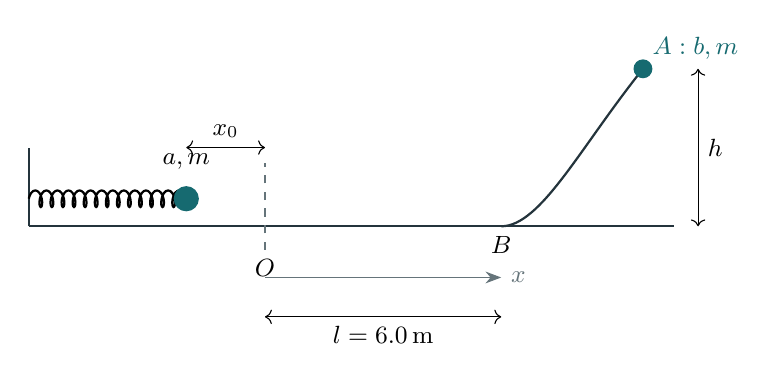
\begin{tikzpicture}[font=\small,spring/.style={decorate,decoration={coil,aspect=.45,segment length=4pt,amplitude=3pt},thick}]
\draw[object](-1,0)--(7.2,0);\draw[object](-1,0)--(-1,1);
\draw[spring](-1,.35)--(1,.35);\fill[accent](1,.35)circle(.16);\node[above]at(1,.6){$a,m$};
\draw[guide](2,-.3)--(2,.8);\node[below]at(2,-.3){$O$};
\draw[object](5,0)..controls(5.5,0)and(6,1)..(6.8,2);
\fill[accent](6.8,2)circle(.12)node[above right]{$A:b,m$};\node[below]at(5,0){$B$};
\draw[<->](1,1)--(2,1)node[midway,above]{$x_0$};
\draw[<->](2,-1.15)--(5,-1.15)node[midway,below]{$l=6.0\,\mathrm m$};
\draw[axis](2,-.65)--(5,-.65)node[right]{$x$};
\draw[<->](7.5,0)--(7.5,2)node[midway,right]{$h$};
\end{tikzpicture}\figcaption{图 7.1}\end{minipage}\end{center}

\Needspace{18\baselineskip}\subsection*{解答}

\begin{center}\begin{minipage}{\linewidth}\centering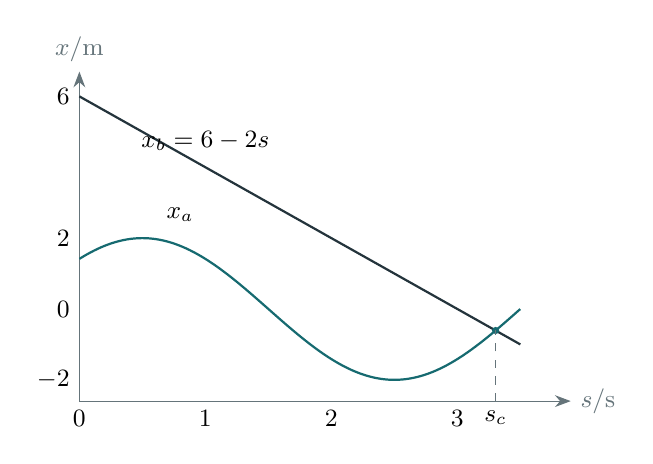
\begin{tikzpicture}[font=\small,x=1.6cm,y=.45cm]
\draw[axis](0,-2.6)--(3.9,-2.6)node[right]{$s/\mathrm s$};
\draw[axis](0,-2.6)--(0,6.7)node[above]{$x/\mathrm m$};
\draw[traj,domain=0:3.5,samples=121]plot(\x,{2*cos(90*\x+315)});
\draw[object](0,6)--(3.5,-1);
\fill[accent](3.303613612,-.607227224)circle(1.3pt);
\draw[guide](3.303613612,-2.6)--(3.303613612,-.607227224);
\node[below]at(3.303613612,-2.6){$s_c$};
\foreach \x in {0,1,2,3}{\node[below]at(\x,-2.6){$\x$};}
\foreach \y in {-2,0,2,6}{\node[left]at(0,\y){$\y$};}
\node[above]at(1,4.2){$x_b=6-2s$};\node[above]at(.8,2.2){$x_a$};
\end{tikzpicture}\figcaption{解图 7.1A}\end{minipage}\end{center}
以平衡点 $O$ 为原点，向右为正；释放时刻记为 $t=0$，碰后另用 $\tau$ 计时。曲面上质点到 $B$ 时由机械能守恒有
\[v_B=\sqrt{2gh}=2.00\,\mathrm{m/s}.\]
它在 $B$ 后向左匀速运动。令 $s=t-t_{AB}\ge0$，两质点的坐标分别为
\[x_b(s)=6-2s,\qquad x_a(s)=-2\cos\left[\frac\pi2(1.5+s)\right]
=2\cos\left(\frac\pi2s+\frac{7\pi}4\right).\]
解图7.1A中直线与正弦曲线的第一次交点才是实际碰撞。方程为
\[6-2s=2\cos\left(\frac\pi2s+\frac{7\pi}4\right).\]
按相同时间步长列表，可先夹住交点：
\begin{center}\begin{tabular}{c|rrrrrrrr}
$s/\mathrm s$&0&0.5&1&1.5&2&2.5&3&3.5\\\hline
$x_b/\mathrm m$&6&5&4&3&2&1&0&$-1$\\
$x_a/\mathrm m$&1.414&2&1.414&0&$-1.414$&$-2$&$-1.414$&0
\end{tabular}\end{center}
$s<2$ 时来球尚在振子右侧；$2\le s\le3$ 时来球非负而振子非正。第一次相遇在 $(3,3.5)$。这段内 $x_b-x_a$ 严格递减，故根唯一。用二分或牛顿迭代求出 $s_c$，再计算
\[t_c=1.5+s_c,\quad x_c=6-2s_c,\quad
v_a=\pi\sin\left[\frac\pi2(1.5+s_c)\right].\]
碰撞期间弹簧冲量可忽略，水平方向动量守恒：
\[2m v_c=m v_a-m v_B,\qquad v_c=\frac{v_a-v_B}{2}.\]
质量变为 $2m$ 后圆频率为 $\omega'=\omega/\sqrt2=\pi/(2\sqrt2)$。因此取碰撞为 $\tau=0$，最直接的表达式为
\[\boxed{x(\tau)=x_c\cos(\omega'\tau)+\frac{v_c}{\omega'}\sin(\omega'\tau).}\]
它在零时刻同时满足 $x(0)=x_c$、$\dot x(0)=v_c$。若改写为 $A\cos(\omega'\tau+\phi)$，则
\[A=\sqrt{x_c^2+(v_c/\omega')^2},\qquad
\phi=\operatorname{atan2}(-v_c/\omega',x_c)\pmod{2\pi}.\]
\begin{center}\begin{minipage}{\linewidth}\centering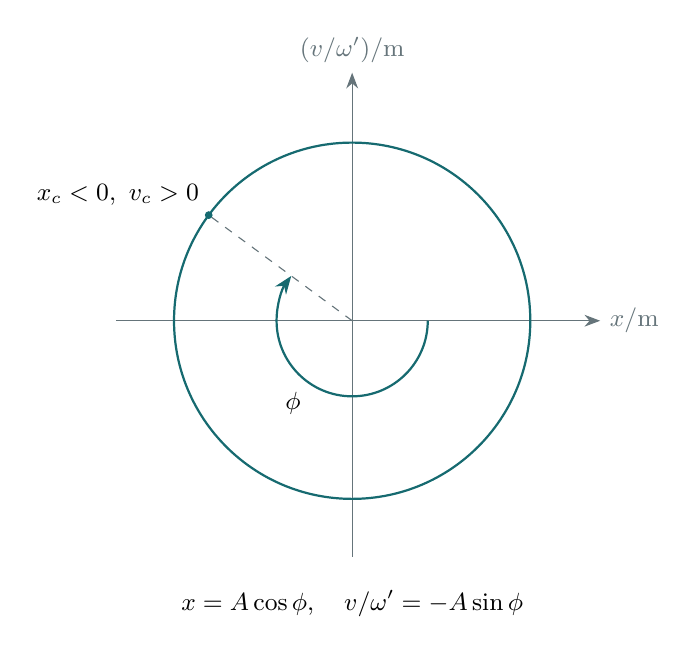
\begin{tikzpicture}[font=\small,x=3cm,y=3cm]
\draw[axis](-1,0)--(1.05,0)node[right]{$x/\mathrm m$};
\draw[axis](0,-1)--(0,1.05)node[above]{$(v/\omega')/\mathrm m$};
\draw[traj](0,0)circle(.754094661);
\fill[accent](-.607227224,.447139638)circle(1.4pt);
\draw[guide](0,0)--(-.607227224,.447139638);
\node[above left]at(-.607227224,.447139638){$x_c<0,\ v_c>0$};
\draw[motion](.32,0)arc(0:-216.3666:.32);
\node at(-.25,-.35){$\phi$};
\node[below]at(0,-1.1){$x=A\cos\phi,\quad v/\omega'=-A\sin\phi$};
\end{tikzpicture}\figcaption{解图 7.1B}\end{minipage}\end{center}
解图7.1B中的初始相点位于 $x<0,v>0$ 区域，满足 $\cos\phi<0,\sin\phi<0$，因此余弦相位在第三象限。下面用交点的未舍入数值计算振幅与相位。
\[\begin{aligned}s_c&=3.303614\,\mathrm s,&t_c&=4.803614\,\mathrm s,\\x_c&=-0.607227\,\mathrm m,&v_a&=2.993295\,\mathrm{m/s},\\v_c&=0.496647\,\mathrm{m/s},&A&=0.754095\,\mathrm m,\\\phi&=3.776309\,\mathrm{rad}& &=216.3666^\circ.\end{aligned}\]
碰撞损失的机械能为 $m(v_a+v_B)^2/4$；它只发生在粘合过程，碰后振动本身守恒机械能。
\subsubsection*{释放、到达曲面底部和碰撞三个时刻}
图7.1以平衡点$O$为零点，压缩量$x_0$是正的长度，
振子的初始坐标却为$-x_0$。
先由释放位置和速度确定碰前振动的两个积分常数，得
\[
x_a(t)=x_0\cos(\omega t+\phi_0),\qquad
x_a(0)=-x_0,\quad\dot x_a(0)=0,
\]
\[
\cos\phi_0=-1,\quad\sin\phi_0=0,
\quad\phi_0=\pi\pmod{2\pi},\qquad
x_a(t)=-2\cos(\pi t/2).
\]
另一质点沿光滑曲面下滑时，支持力不做功，
$mgh=mv_B^2/2$给$v_B=2\,\mathrm{m/s}$。
下滑高度决定到达 $B$ 时的速率，曲面的形状还影响滑行历时。本题直接给出这段历时为 $t_{AB}=1.5\,\mathrm s$。
到达$B$后才作向左匀速运动，因此其位置和速度初值应在$t_{AB}=1.5\,\mathrm s$处接续。
令$s=t-t_{AB}$，代入振子方程的相位应逐项为
\[
\omega(t_{AB}+s)+\pi
=\frac\pi2s+\frac34\pi+\pi
=\frac\pi2s+\frac74\pi.
\]
这样在 $s=0$ 时，振子已经运动 $t_{AB}$，位置和速度从释放状态接续而来。

\subsubsection*{第一次相遇的筛选和数值迭代}
解图7.1A的两条曲线按同一时间、位置刻度绘制。
设$F(s)=x_b(s)-x_a(s)$。
对$0\leq s<2$，$x_b>2\,\mathrm m$而$x_a\leq2\,\mathrm m$，没有相遇；
$s=2$时$x_b=2$、$x_a=-\sqrt2$，也不相等。
在$2\leq s\leq3$上，$x_b\geq0$而$x_a<0$，仍不相遇。
接着计算
\[
F(3)=\sqrt2>0,\qquad F(3.5)=-1<0.
\]
该区间内$\pi s/2+7\pi/4$按$2\pi$约去后位于$[5\pi/4,3\pi/2]$，
所以其正弦为负，
\[
F'(s)=-2+\pi\sin\left(\frac\pi2s+\frac{7\pi}4\right)<-2<0.
\]
因而这里有且仅有一个根，并且就是实际发生的第一次碰撞。
二分法保持$F$异号的两端；若用牛顿法，则迭代式为
\[
s_{n+1}=s_n-
\frac{6-2s_n-2\cos(\pi s_n/2+7\pi/4)}
{-2+\pi\sin(\pi s_n/2+7\pi/4)}.
\]
以$s_0=3.3$起算，可收敛到$s_c=3.303613612\cdots$。
在求根和随后计算中保留这些有效位，最后才按所需精度取值。
将根代回两条轨迹，分别得到同一$x_c$，
而碰前速度须分别求斜率：
\[
\dot x_b=-2,\qquad
\dot x_a=-\pi\sin\left(\frac\pi2s+\frac{7\pi}4\right).
\]
这与$\dot x_a=\pi\sin[\pi(1.5+s)/2]$完全相同，
振子的速度为正，来球速度为负，二者迎面碰撞。动量式中的两个有向速度分别是 $v_a$ 和 $-v_B$。

\subsubsection*{碰后初值、振幅及相位的完整恢复}
碰撞历时远小于振动周期，弹簧在这段时间内可以取碰撞位置处的伸长量。弹簧的冲量可略，两物体以碰前速度的质量加权平均值一同运动。
动量守恒计算的中间数值为
\[
v_c=\frac{2.993294535-2}{2}
=0.496647267\cdots\,\mathrm{m/s},
\qquad \omega'=\frac{\pi}{2\sqrt2}=1.110720735\cdots\,\mathrm{s}^{-1}.
\]
将碰后时间记为$\tau$，线性组合中两项系数由初值分别确定：
\[
x=C_1\cos\omega'\tau+C_2\sin\omega'\tau,
\quad C_1=x_c,
\quad \dot x(0)=\omega'C_2=v_c,
\quad C_2=v_c/\omega'.
\]
因此可直接给出带数值的振动式
\[
x(\tau)=
(-0.607227224\cdots)\cos(1.110720735\cdots\tau)
+(0.447139638\cdots)\sin(1.110720735\cdots\tau)
\quad\mathrm m.
\]
展开幅相式$A\cos(\omega'\tau+\phi)$并逐项比较，
\[
A\cos\phi=x_c<0,\qquad
-A\sin\phi=v_c/\omega'>0.
\]
所以$\cos\phi<0$且$\sin\phi<0$，$\phi$在第三象限，
而解图7.1B中的相点$(x,v/\omega')$在第二象限；
由 $v/\omega^{\prime}=-A\sin\phi$，相点从正横轴量起的极角为 $-\phi$。
\[
\phi=\pi+\arctan\frac{v_c}{\omega'|x_c|}
=3.776308779\cdots\,\mathrm{rad},
\quad A=0.754094661\cdots\,\mathrm m.
\]
据此也可写成$x=A\cos(1.110720735\cdots\tau+3.776308779\cdots)$。
$\cos\phi$ 的符号由左侧位置给出，$\sin\phi$ 的符号由向右的初速度给出。这两个符号将正切相同而相差 $\pi$ 的候选相位区分开。

\subsubsection*{碰撞损失与后续振动能量}
碰撞前后弹簧势能相同，故失能只由两质点动能差计算：
\[
\begin{aligned}
Q&=\frac m2(v_a^2+v_B^2)
-\frac12(2m)\left(\frac{v_a-v_B}{2}\right)^2\\
&=\frac m4(v_a^2+2v_av_B+v_B^2)
=\frac m4(v_a+v_B)^2>0.
\end{aligned}
\]
碰后则是质量$2m$的单一振子，
\[
E_f=mv_c^2+\frac12kx_c^2
=\frac12k\left(x_c^2+\frac{v_c^2}{\omega'^2}\right)
=\frac12kA^2.
\]
第一式用$2m$计平动能，第二式代入 $k=2m\omega^{\prime 2}$ 将速度项改写为位移平方。
碰撞中的动能损失与碰后振动的机械能守恒属于不同时间段。


\Needspace{18\baselineskip}

\pdfbookmark[2]{第 2 题 密度线性分层液体中的浮力振动}{q2}

\section*{第 2 题\quad 密度线性分层液体中的浮力振动}

\tagline{M-07-02}

如图,某液体的密度随深度线性地增加,液体表面的密度为\(\rho_{0}\),深度为\(D\)处的密度为\(2\rho_{0}\),一密度为\(2\rho_{0}\)的小球在深度为\(\frac{D}{2}\)处从静止释放.忽略液体的阻力.试求小球的振动表达式.

小球尺度远小于密度变化长度；密度规律在运动所达深度内成立，忽略液体附加质量。

\begin{center}\begin{minipage}{\linewidth}\centering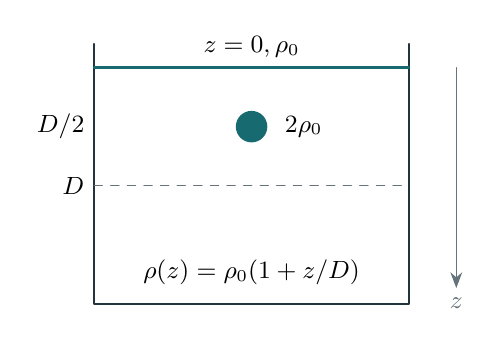
\begin{tikzpicture}[line cap=round,line join=round,spring/.style={decorate,decoration={coil,aspect=.45,segment length=4pt,amplitude=3pt},thick}]\draw[object] (0,3)--(0,-.3)--(4,-.3)--(4,3);\draw[traj] (0,2.7)--(4,2.7);\node[above] at (2,2.7) {$z=0,\rho_0$};\draw[axis] (4.6,2.7)--(4.6,-.1) node[below] {$z$};\draw[guide](0,1.2)--(4,1.2);\node[left]at(0,1.2){$D$};\fill[accent] (2,1.95) circle (.2);\node[right] at (2.3,1.95) {$2\rho_0$};\node[left] at (0,1.95) {$D/2$};\node at (2,.1) {$\rho(z)=\rho_0(1+z/D)$};\end{tikzpicture}\figcaption{图 7.2}\end{minipage}\end{center}

\Needspace{18\baselineskip}\subsection*{解答}

\begin{center}\begin{minipage}{\linewidth}\centering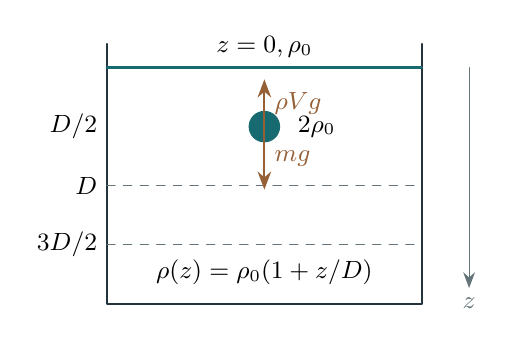
\begin{tikzpicture}[line cap=round,line join=round,spring/.style={decorate,decoration={coil,aspect=.45,segment length=4pt,amplitude=3pt},thick}]\draw[object] (0,3)--(0,-.3)--(4,-.3)--(4,3);\draw[traj] (0,2.7)--(4,2.7);\node[above] at (2,2.7) {$z=0,\rho_0$};\draw[axis] (4.6,2.7)--(4.6,-.1) node[below] {$z$};\draw[guide] (0,1.2)--(4,1.2);\node[left]at(0,1.2){$D$};\fill[accent] (2,1.95) circle (.2);\node[right] at (2.3,1.95) {$2\rho_0$};\node[left] at (0,1.95) {$D/2$};\node at (2,.1) {$\rho(z)=\rho_0(1+z/D)$};\draw[force](2,1.95)--(2,1.15)node[midway,right]{$mg$};\draw[force](2,1.95)--(2,2.55)node[midway,right]{$\rho Vg$};\draw[guide] (0,.45)--(4,.45);\node[left]at(0,.45){$3D/2$};\end{tikzpicture}\figcaption{解图 7.2A}\end{minipage}\end{center}
解图7.2A以液面为零深度，$z$ 向下为正。线性密度规律由两个给定值确定：
\[\rho(z)=\rho_0+\frac{\rho_0}{D}z=\rho_0(1+z/D).\]
设球体积为 $V$，质量为 $m=2\rho_0V$。重力向下，浮力向上，故
\[m\ddot z=mg-\rho(z)Vg
=\rho_0Vg(1-z/D),\qquad
\ddot z+\frac g{2D}(z-D)=0.\]
浮力所用的密度是小球所在深度的液体密度。若球从$z$向下再移$\Delta z$，重力不变，浮力增加$\rho_0Vg\Delta z/D$，因而合力变化为
\[\Delta F_z=-\frac{\rho_0Vg}{D}\Delta z.\]
这个负斜率给回复系数$K=\rho_0Vg/D$；除以球自身质量$2\rho_0V$才得到$\omega^2$。给定密度在所用液层中为线性函数，所以回复合力在整个运动范围内都与 $x$ 成正比。

平衡深度为 $z_e=D$。令 $x=z-D$，才有齐次的简谐方程
\[\ddot x+\omega^2x=0,\qquad\omega=\sqrt{g/(2D)}.\]
从深度 $D/2$ 静止释放，初值是 $x(0)=-D/2$、$\dot x(0)=0$，因此
\[x(t)=-\frac D2\cos(\omega t),\qquad
\boxed{z(t)=D-\frac D2\cos\left(\sqrt{\frac g{2D}}t\right).}\]
解图7.2A的初始位置在平衡点上方，故$z(0)<D$时向下合力为正，初始加速度应向下。由解得
\[\dot z=\frac D2\omega\sin\omega t,
\qquad \dot z(T/4)=\frac D2\omega=\sqrt{gD/8}.\]
四分之一周期到达平衡点时速率最大，半周期到图中的深端并瞬时停下。余弦项在初始时取负值，表示从上方浅端释放。

解图中的两个转折深度为 $D/2$ 与 $3D/2$，相应平衡位移为 $-D/2$ 与 $D/2$。液面深度由平衡位移加上 $D$ 得到。本题按小球自身质量计惯性，线性密度规律覆盖它经过的整个液层。
也可定义相对于平衡的有效势能 $U=\rho_0Vg x^2/(2D)$；由 $m\dot x^2/2+U$ 守恒得到同一频率。
\subsubsection*{合力、平衡位移和释放初值的逐步代入}
解图7.2A的$z$从液面向下量，$x=z-D$从平衡深度量。
在同一初态，两种坐标分别是$z_0=D/2$和$x_0=-D/2$。
先代质量和密度，再约去共同的$\rho_0V$，
\[
2\rho_0V\ddot z=2\rho_0Vg-
\rho_0\left(1+\frac zD\right)Vg,
\]
\[
\ddot z=\frac g2-\frac g{2D}z
=-\frac g{2D}(z-D).
\]
因此在液面下深度 $D$ 处浮力与重力相等。
令$x=A\cos(\omega t+\phi)$，
释放条件给
\[
A\cos\phi=-D/2,\qquad -A\omega\sin\phi=0,
\quad A=D/2,\quad\phi=\pi.
\]
这恢复$x=-(D/2)\cos\omega t$，加回$D$才是题目所问的液面下深度。
周期为$T=2\pi\sqrt{2D/g}$；频率量纲为$1/\mathrm s$，与球体积无关。

\subsubsection*{浅端、平衡点与深端的浮力和速率}
初态$z=D/2$处液体密度为$3\rho_0/2$，
浮力与重力之比是$3/4$，故初始向下加速度为$g/4$。
在$z=D$，两力相等、加速度为零，但速率最大；
在$z=3D/2$，浮力与重力之比为$5/4$，加速度为向上的$g/4$，
速度则在转折瞬间为零。
在解图7.2B中，曲线从浅端以零斜率出发，深度随向下加速而增加。过平衡深度时斜率绝对值最大，到深端时斜率降为零，随后开始上浮。
\begin{center}\begin{minipage}{\linewidth}\centering
\begin{tikzpicture}[x=.95cm,y=1.65cm,font=\small]
\draw[axis](0,.25)--(6.7,.25)node[right]{$\omega t$};
\draw[axis](0,.25)--(0,1.85)node[above]{$z/D$};
\draw[traj,domain=0:6.283185307,samples=101]plot(\x,{1-.5*cos(\x*180/pi)});
\draw[guide](0,1)--(6.283185307,1);
\foreach \x/\lab in {1.570796327/{\pi/2},3.141592654/{\pi},4.712388980/{3\pi/2},6.283185307/{2\pi}}
 {\draw(\x,.25)--(\x,.2);\node[below]at(\x,.2){$\lab$};}
\foreach \y/\lab in {.5/{1/2},1/{1},1.5/{3/2}}{\node[left]at(0,\y){$\lab$};}
\fill(0,.5)circle(1.1pt);\fill(3.141592654,1.5)circle(1.1pt);
\node[above]at(3.141592654,1.5){最深，$v=0$};
\end{tikzpicture}
\figcaption{解图7.2B\quad 深度先增后减，过平衡位置时曲线的斜率绝对值最大。}
\end{minipage}\end{center}
回复合力$F_z=-Kx$对应
\[
K=\frac{\rho_0Vg}{D},\qquad
U(x)=\int_0^x K\xi\dd\xi=\frac12Kx^2.
\]
从静止释放，能量常数为
\[
E=\frac12K(D/2)^2=\frac{\rho_0VgD}{8}
=\frac{mgD}{16}.
\]
到平衡点时$U=0$，$mv_{\max}^2/2=mgD/16$给
$v_{\max}=\sqrt{gD/8}$，与对振动式求导相同。
另一转折点满足同一$U$而位移反号，故$x=D/2$、$z=3D/2$。

\subsubsection*{液面、底部和密度模型的范围}
小球的中心运动范围为$D/2\leq z\leq3D/2$。
若球的半径为 $r$，浅端的球顶深度为 $D/2-r$，深端的球底深度为 $3D/2+r$。前者为正、后者小于容器深度，给出完全浸没且无底面接触的范围。题设用无阻力、无附加质量的小球模型，因而回复系数除以球自身质量得到频率。


\Needspace{18\baselineskip}

\pdfbookmark[2]{第 3 题 两滚轮支承木板的微小振动}{q3}

\section*{第 3 题\quad 两滚轮支承木板的微小振动}

\tagline{M-07-03}

如图7.3,两个完全相同的圆柱状滚轮在水平面内平行放置,各绕自身的轴线按图示方向等角速转动,两轴线之间的距离为\(2l\).在两滚轮上平放一块重量为\(G\)的均匀木板,木板与滚轮之间的摩擦系数为\(\mu\).若木板重心偏离两轴中心位置一个微小的距离,试描述木板的运动.

左轮顶面向右、右轮顶面向左。木板视为薄板，微小振动时两接触始终滑动且摩擦方向保持不变。

\begin{center}\begin{minipage}{\linewidth}\centering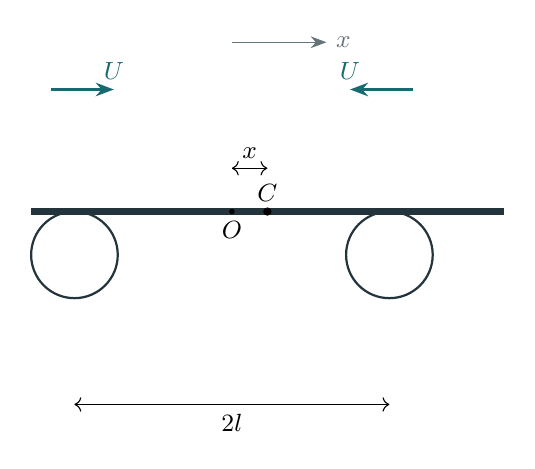
\begin{tikzpicture}[font=\small]
\draw[object,fill=white](0,0)circle(.55);\draw[object,fill=white](4,0)circle(.55);
\draw[object,line width=2.5pt](-.55,.55)--(5.45,.55);
\fill(2.45,.55)circle(1.5pt)node[above]{$C$};\fill(2,.55)circle(1pt)node[below]{$O$};
\draw[motion](-.3,2.1)--(.5,2.1)node[above]{$U$};
\draw[motion](4.3,2.1)--(3.5,2.1)node[above]{$U$};
\draw[axis](2,2.7)--(3.2,2.7)node[right]{$x$};
\draw[<->](0,-1.9)--(4,-1.9)node[midway,below]{$2l$};
\draw[<->](2,1.1)--(2.45,1.1)node[midway,above]{$x$};
\end{tikzpicture}\figcaption{图 7.3}\end{minipage}\end{center}

\Needspace{18\baselineskip}\subsection*{解答}

\begin{center}\begin{minipage}{\linewidth}\centering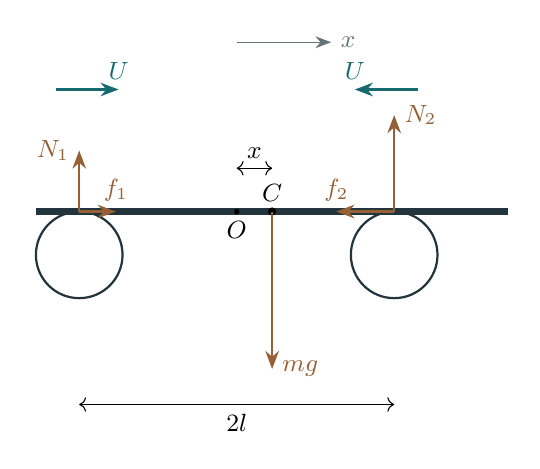
\begin{tikzpicture}[font=\small]
\draw[object,fill=white](0,0)circle(.55);\draw[object,fill=white](4,0)circle(.55);
\draw[object,line width=2.5pt](-.55,.55)--(5.45,.55);
\fill(2.45,.55)circle(1.5pt)node[above]{$C$};\fill(2,.55)circle(1pt)node[below]{$O$};
\draw[motion](-.3,2.1)--(.5,2.1)node[above]{$U$};
\draw[motion](4.3,2.1)--(3.5,2.1)node[above]{$U$};
\draw[axis](2,2.7)--(3.2,2.7)node[right]{$x$};
\draw[<->](0,-1.9)--(4,-1.9)node[midway,below]{$2l$};
\draw[<->](2,1.1)--(2.45,1.1)node[midway,above]{$x$};
\draw[force](0,.55)--(0,1.325)node[left]{$N_1$};
\draw[force](4,.55)--(4,1.775)node[right]{$N_2$};
\draw[force](2.45,.55)--(2.45,-1.45)node[right]{$mg$};
\draw[force](0,.55)--(.465,.55)node[above]{$f_1$};
\draw[force](4,.55)--(3.265,.55)node[above]{$f_2$};
\end{tikzpicture}\figcaption{解图 7.3A}\end{minipage}\end{center}
取两轮中点为 $O$，质心偏移 $x$ 向右为正。左轮顶面向右、右轮顶面向左，故木板受 $f_1=\mu N_1$ 向右、$f_2=\mu N_2$ 向左。薄板竖直方向平衡且不俯仰：
\[N_1+N_2=mg,\qquad N_1(l+x)=N_2(l-x).\]
取木板质心为力矩中心时，左支持点在它左侧$l+x$处，右支持点在它右侧$l-x$处。重力通过质心不贡献力矩，故两支持力的力矩大小相等。将$N_2=mg-N_1$代入，
\[N_1(l+x)=(mg-N_1)(l-x)
\ \Longrightarrow\ 2lN_1=mg(l-x).\]
载荷随质心位置重新分配，中心位置 $x=0$ 对应两轮各承担一半重量。

解得
\[N_1=\frac{mg}{2}(1-x/l),\qquad
N_2=\frac{mg}{2}(1+x/l).\]
解图7.3A显示向右偏移后右轮承重增大；其向左摩擦也增大。于是
\[m\ddot x=f_1-f_2=\mu(N_1-N_2)=-\frac{\mu mg}{l}x.\]
从 $x(0)=a$ 静止释放时
\[\boxed{x(t)=a\cos\left(\sqrt{\frac{\mu g}{l}}t\right),\quad
T=2\pi\sqrt{\frac l{\mu g}}.}\]
解图7.3A中的两个摩擦力始终分别由轮面相对木板的滑动决定。当$x>0$时，$N_2>N_1$，合力向左；当$x<0$时则反向，故合力总与位移反向。将运动方程写成$\ddot x+\Omega^2x=0$，再以初值确定余弦项，所得周期与木板质量无关，是因为载荷产生的摩擦和木板惯性都正比于$m$。驱动装置持续维持两轮转速，两接触持续滑动。装置输入的功率分配给木板动能的变化和接触发热。

取振幅为 $|a|$，两轮都保持正压力时 $|a|<l$。最大板速 $|a|\sqrt{\mu g/l}$ 小于轮顶速率时，两接触的滑动方向在整个周期内均保持图示方向，两支摩擦分别向右和向左。
\subsubsection*{力臂、压力和回复力的全步消元}
图7.3和解图7.3A均以两轮中点为$O$，$C$向右偏$x>0$。
均匀板的几何中心与质心重合，$x$ 同时描述整块木板相对于两轮的水平移动。
左、右支点相对$C$的坐标是$-(l+x)$与$l-x$。
薄板近似把水平摩擦的竖直力臂忽略，支持力矩平衡给
\[
N_1(l+x)=N_2(l-x),\qquad N_2=mg-N_1.
\]
展开右端并把两项$N_1$合并，
\[
N_1[(l+x)+(l-x)]=mg(l-x),\quad
N_1=\frac{mg(l-x)}{2l},
\]
\[
N_2=mg-\frac{mg(l-x)}{2l}
=\frac{mg(l+x)}{2l},\qquad N_1-N_2=-\frac{mg}{l}x.
\]
左轮顶面相对板向右滑，右轮顶面相对板向左滑，
所以取向右为正时，合力为$\mu N_1-\mu N_2$。
两处的相对滑动方向给出水平方向合力的正负号。
\begin{center}\begin{minipage}{\linewidth}\centering
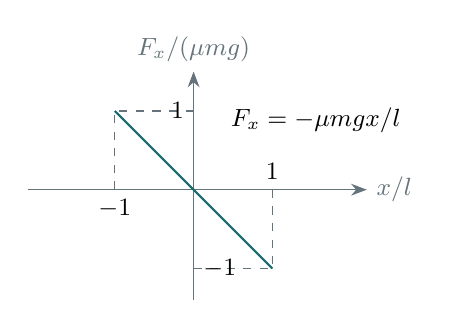
\begin{tikzpicture}[font=\small]
\draw[axis](-2.1,0)--(2.2,0)node[right]{$x/l$};
\draw[axis](0,-1.4)--(0,1.5)node[above]{$F_x/(\mu mg)$};
\draw[traj](-1,1)--(1,-1);
\draw[guide](-1,0)--(-1,1)--(0,1);
\draw[guide](1,0)--(1,-1)--(0,-1);
\node[below]at(-1,0){$-1$};\node[above]at(1,0){$1$};
\node[left]at(0,1){$1$};\node[right]at(0,-1){$-1$};
\node[above right]at(.35,.6){$F_x=-\mu mgx/l$};
\end{tikzpicture}
\figcaption{解图7.3B\quad 固定滑动方向下的回复合力；端点对应左轮或右轮支持力为零。}
\end{minipage}\end{center}
于是$\Omega^2=\mu g/l$，一般初值$x_i,v_i$给
\[
x=x_i\cos\Omega t+\frac{v_i}{\Omega}\sin\Omega t,
\quad A=\sqrt{x_i^2+(v_i/\Omega)^2},\quad v_{\max}=A\Omega.
\]
静止偏移释放只是$v_i=0$的特例。

\subsubsection*{振幅、轮速及有限板长的共同限制}
两接触的相对滑速分别为$U-\dot x$和$-U-\dot x$，
$U>0$是两轮顶面速率。
两接触的滑速分别保持一正一负，给出 $-U<\dot x<U$。用全程最大速率与振幅表示，得到
\[
A\Omega<U,\qquad A<l.
\]
前一条件防止相对滑动反向，后一条件保证两个支持力都严格为正。
若均匀板总长为$L_b$，还需两个滚轮始终落在板的范围内：
\[
L_b/2>l+A.
\]
严格大于时，两个支点在每个转折位置仍位于板内；板的几何范围、两处正压力和相对滑速共同确定这段振动所适用的振幅。

\subsubsection*{驱动功、木板动能和接触发热}
解图7.3A两轮由装置维持$+U,-U$的顶面速度。
木板所受功率为
\[
P_{\rm board}=(f_1-f_2)\dot x
=-\frac{\mu mg}{l}x\dot x=\frac{\dd K_{\rm board}}{\dd t}.
\]
它随位置、速度的乘积变号，摩擦可使板加速也可使板减速。
两轮受到相反的接触反力，维持轮速所需的驱动功率为
\[
P_{\rm drive}=U(f_1+f_2)=\mu mgU.
\]
滑动发热率逐接触相加为
\[
\dot Q=f_1(U-\dot x)+f_2(U+\dot x)
=\mu mgU-(f_1-f_2)\dot x.
\]
故$P_{\rm drive}=\dot Q+\dot K_{\rm board}$，
在所给速度范围内每一接触的发热都非负。
板的方程还可积分成
$K_{\rm board}+\mu mgx^2/(2l)=\text{常量}$，
其中第二项由净回复力对位置积分而定义，它将木板的运动方程写成能量积分的形式。
一完整周期内板动能回到初值，驱动做功$\mu mgUT$全部成为接触热量。


\Needspace{18\baselineskip}

\pdfbookmark[2]{第 4 题 地球贯通隧道中的简谐运动}{q4}

\section*{第 4 题\quad 地球贯通隧道中的简谐运动}

\tagline{M-07-04}

牛顿曾证明:一个均匀球壳,对球壳内物质的万有引力为零,而对球壳外物质的万有引

力不为零,并且其作用就相当于球壳的质量都集中到球心那样(参看力学第三章题11).如图所示,设想沿地球直径开凿一条贯通地球的隧道,将一小球从洞口由静止释放,试求小球到达隧道另一洞口所用的时间.已知地球的半径为\(R\),质量为\(M\),设地球的质量均匀分布.

忽略地球自转、空气阻力及开凿对质量分布的影响。

\begin{center}\begin{minipage}{\linewidth}\centering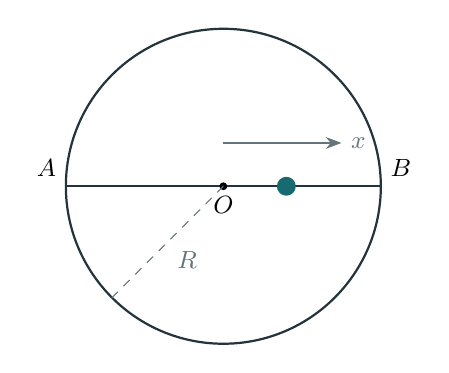
\begin{tikzpicture}[line cap=round,line join=round,spring/.style={decorate,decoration={coil,aspect=.45,segment length=4pt,amplitude=3pt},thick}]\draw[object] (0,0) circle (2);\draw[object] (-2,0)--(2,0);\fill[accent] (.8,0) circle (.12);\fill (0,0) circle (.05);\draw[axis] (0,.55)--(1.5,.55) node[right] {$x$};\node[below] at (0,0) {$O$};\node[above left] at (-2,0) {$A$};\node[above right] at (2,0) {$B$};\draw[guide] (0,0)--(-1.414213562,-1.414213562) node[midway,below right] {$R$};\end{tikzpicture}\figcaption{图 7.4}\end{minipage}\end{center}

\Needspace{18\baselineskip}\subsection*{解答}

\begin{center}\begin{minipage}{\linewidth}\centering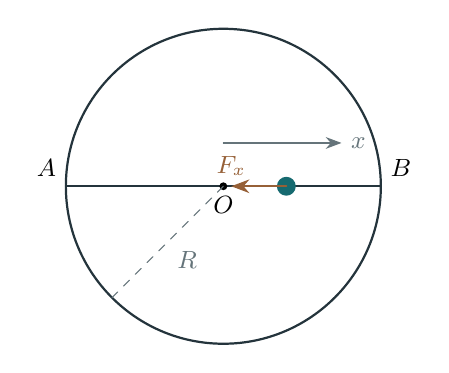
\begin{tikzpicture}[line cap=round,line join=round,spring/.style={decorate,decoration={coil,aspect=.45,segment length=4pt,amplitude=3pt},thick}]\draw[object] (0,0) circle (2);\draw[object] (-2,0)--(2,0);\fill[accent] (.8,0) circle (.12);\fill (0,0) circle (.05);\draw[axis] (0,.55)--(1.5,.55) node[right] {$x$};\node[below] at (0,0) {$O$};\node[above left] at (-2,0) {$A$};\node[above right] at (2,0) {$B$};\draw[guide] (0,0)--(-1.414213562,-1.414213562) node[midway,below right] {$R$};\draw[force] (.8,0)--(.1,0) node[above] {$F_x$};\end{tikzpicture}\figcaption{解图 7.4A}\end{minipage}\end{center}
在地球内部，半径 $r$ 以内的质量为
\[M(r)=\frac{M}{4\pi R^3/3}\frac{4\pi r^3}{3}=M\frac{r^3}{R^3}.\]
外侧球壳的合引力为零。以球心为原点，隧道坐标 $x$ 为有符号量，球受力为
\[F_x=-\frac{GMm}{R^3}x,\qquad
\ddot x+\frac{GM}{R^3}x=0.\]
解图7.4A的力箭头始终指向球心，力的大小与偏心距离成正比；取右洞口$B$为释放处。由 $x(0)=R$、$\dot x(0)=0$，
\[x(t)=R\cos(\omega t),\quad\omega=\sqrt{GM/R^3},\quad
T=2\pi\sqrt{R^3/(GM)}.\]
到另一洞口 $x=-R$ 是第一次达到另一端点，耗时半周期：
\[\boxed{t_{\text{穿越}}=\pi\sqrt{\frac{R^3}{GM}}=\pi\sqrt{\frac R{g_s}},\qquad g_s=GM/R^2.}\]
由能量求得球心速率为 $v_{\max}=\omega R=\sqrt{GM/R}$。地表圆轨道速度也是该值，走半圆的时间 $\pi R/v_{\max}$ 与穿越时间相同；圆周运动投影到直径即为此简谐轨迹。这一等时关系由均匀密度下的线性引力和非旋转模型给出。
若把隧道改为距地心 $b<R$ 的任意弦，以弦中点为坐标原点，则 $\mathbf r=x\hat{\mathbf e}_x+b\hat{\mathbf e}_b$。球内引力的向量式为 $\mathbf F=-m\omega^2\mathbf r$，沿弦仍有 $F_x=-m\omega^2x$；壁的支持力抵消横向分量，大小 $m\omega^2b$，不做功。两洞口坐标为 $x=\pm\sqrt{R^2-b^2}$，振幅改为 $\sqrt{R^2-b^2}$，频率与端到端的半周期不变，最大速度却随弦长减小。解图7.4B把沿弦分量与横向分量分别画出。
\subsubsection*{半径与有符号隧道坐标的区别}
解图7.4A取右洞口$B$为释放处，$x(0)=R$。
半径$r=|x|\geq0$用于计算球内包围质量，
而运动方程用可正可负的$x$，过球心后无需重设正方向。
先由均匀密度逐项消去体积因子，
\[
\rho=\frac{M}{4\pi R^3/3},\qquad
M(r)=\rho\frac{4\pi r^3}{3}=M\frac{r^3}{R^3}.
\]
外侧每一完整球壳对内部小球的合引力都为零，
内侧球体的作用等效于其质量集中在球心。
在$r>0$处，
\[
\boldsymbol F=-\frac{GmM(r)}{r^3}\boldsymbol r
=-\frac{Gm}{r^3}\frac{Mr^3}{R^3}\boldsymbol r
=-\frac{GMm}{R^3}\boldsymbol r.
\]
约去 $r^3$ 后，引力与位矢成正比，在 $r=0$ 连续取零。
沿直径投影再除以$m$，得到$\ddot x+\omega^2x=0$。
这里均匀密度使 $M(r)/r^3=M/R^3$ 成为常量，从而产生线性回复力。

\subsubsection*{从一侧洞口到地心和另一侧洞口的时间}
齐次方程的一般解为$C_1\cos\omega t+C_2\sin\omega t$。
释放条件分别给$C_1=R$、$\omega C_2=0$，故$x=R\cos\omega t$。
第一次到达另一洞口要求$\cos\omega t=-1$，
最小正解为$\omega t=\pi$。地心在两个洞口之间，第一次到地心的时刻为$\pi/(2\omega)$，再经过同样长的时间到另一侧洞口。
在两端，速度为零而加速度朝地心；在地心，速度最大而加速度为零。

引力在直径上的势能差为
\[
U(x)-U(0)=\int_0^x m\omega^2\xi\dd\xi
=\frac12m\omega^2x^2.
\]
以洞口初态作能量常数，
\[
\frac12m\dot x^2+\frac12m\omega^2x^2
=\frac12m\omega^2R^2,
\qquad \dot x=-\omega\sqrt{R^2-x^2}.
\]
负号对应从右洞口向左运动。
用上面的速度将时间写成位移积分，从右侧洞口$R$积到左侧洞口$-R$：
\[
t=\int_R^{-R}\frac{-\dd x}{\omega\sqrt{R^2-x^2}}
=\frac1\omega\left[\arcsin\frac xR\right]_{-R}^{R}
=\frac\pi\omega.
\]
在两端附近，速度按到端点距离的平方根减小。因此时间被积函数虽在端点发散，积分仍收敛。
球心速率$\omega R$与地表圆轨道速率相同，
圆轨道的半圈时间因此也为$\pi/\omega$。
两种运动在直径上的坐标满足同一方程和同一初值，因此投影轨迹相同。

\subsubsection*{任意弦的力分解及模型范围}
解图7.4B取弦中点为$H$，$OH=b$，
沿弦坐标为$x$；相对球心的距离满足$r^2=x^2+b^2$。
\begin{center}\begin{minipage}{\linewidth}\centering
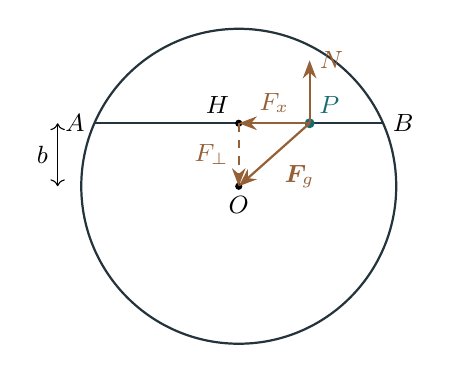
\begin{tikzpicture}[font=\small]
\draw[object](0,0)circle(2);
\draw[object](-1.833030278,.8)--(1.833030278,.8);
\fill(0,0)circle(1.3pt)node[below]{$O$};
\fill(0,.8)circle(1.3pt)node[above left]{$H$};
\fill[accent](.9,.8)circle(1.8pt)node[above right]{$P$};
\draw[force](.9,.8)--(0,0)node[midway,below right]{$\boldsymbol F_g$};
\draw[force](.9,.8)--(0,.8)node[midway,above]{$F_x$};
\draw[force,dashed](0,.8)--(0,0)node[midway,left]{$F_\perp$};
\draw[force](.9,.8)--(.9,1.6)node[right]{$N$};
\draw[<->](-2.3,0)--(-2.3,.8)node[midway,left]{$b$};
\node[left]at(-1.833030278,.8){$A$};\node[right]at(1.833030278,.8){$B$};
\end{tikzpicture}
\figcaption{解图7.4B\quad 弦隧道变式；沿弦回复力指向$H$，横向引力由光滑壁的支持力抵消。}
\end{minipage}\end{center}
球内引力为$-m\omega^2\boldsymbol r$，
两个分量分别是$F_x=-m\omega^2x$与$F_\perp=-m\omega^2b$。
光滑壁给$N=m\omega^2b$，其方向与沿弦速度垂直，不做功。
所以弦的半长虽变为$A=\sqrt{R^2-b^2}$，
时间积分仍是$\int_{-A}^{A}\dd x/[\omega\sqrt{A^2-x^2}]=\pi/\omega$。
行程 $2A$ 与最大速率 $\omega A$ 均按半弦长缩放，所以比值与 $A$ 无关。

均匀密度、忽略自转与阻力、隧道足够窄而不改变球体质量分布，
是上述理想模型的条件。
进入球面时取 $t=0$，令入球位置的有向隧道坐标为 $x_i$、沿隧道的有向速度为 $u_i$。回到球面的这段球内运动可写成 $x=x_i\cos\omega t+(u_i/\omega)\sin\omega t$，其中随时有 $r\leq R$。


\Needspace{18\baselineskip}

\pdfbookmark[2]{第 5 题 斜面上弹簧连接滚动圆柱的振动周期}{q5}

\section*{第 5 题\quad 斜面上弹簧连接滚动圆柱的振动周期}

\tagline{M-07-05}

如图7.5,在倾角为\(\theta\)的斜面上有一劲度系数为\(k\)的弹簧,一端固定,另一端与质量为\(m\)的实心圆柱体的轴连接,圆柱体在斜面上作纯滚动.忽略轴承的摩擦.试求振动周期.

\begin{center}\begin{minipage}{\linewidth}\centering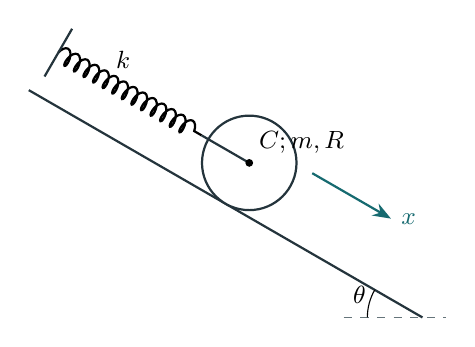
\begin{tikzpicture}[font=\small,spring/.style={decorate,decoration={coil,aspect=.45,segment length=4pt,amplitude=3pt},thick}]
\coordinate(P)at(.5,-.288675135);\coordinate(C)at(.8,.230940108);\coordinate(S)at(-1.624871131,1.630940108);\coordinate(E)at(.193782217,.580940108);
\draw[object](-2,1.154700538)--(3,-1.732050808);\draw[guide](2,-1.732050808)--(3.3,-1.732050808);
\draw[object,fill=white](C)circle(.6);\draw[spring](S)--(E);\draw[object](E)--(C);
\draw[object](-1.799871131,1.327831217)--(-1.449871131,1.934048999);
\fill(C)circle(1.4pt);\node[above right]at(C){$C;m,R$};\node[above]at(-.8,1.3){$k$};
\draw[motion](1.6,.1)--(2.6,-.477350269)node[right]{$x$};
\draw(2.3,-1.732050808)arc(180:150:.7);\node at(2.2,-1.45){$\theta$};
\end{tikzpicture}\figcaption{图 7.5}\end{minipage}\end{center}

\Needspace{18\baselineskip}\subsection*{解答}

\begin{center}\begin{minipage}{\linewidth}\centering\begin{tikzpicture}[font=\small]
\coordinate(P)at(.5,-.288675135);\coordinate(C)at(.8,.230940108);
\draw[object](-2,1.154700538)--(3,-1.732050808);\draw[object](C)circle(.6);
\fill(C)circle(1.4pt)node[below left]{$C$};\node[below left]at(P){$P$};
\draw[force](C)--(-1.278460969,1.430940108)node[above left]{$k(x_0+x)$};
\draw[force](C)--(1.579422863,1.580940108)node[right]{$N$};
\draw[force](C)--(.8,-1.569059892)node[below right]{$mg$};
\draw[force](P)--(.933012702,-.538675135)node[right]{$f$};
\node[align=left,anchor=west]at(2,1.4){$x>0$\\$f>0$向下坡};
\end{tikzpicture}\figcaption{解图 7.5A}\end{minipage}\end{center}
取下坡方向为正，$x$ 从圆柱平衡位置量起，弹簧平衡伸长为 $x_0$。静态时摩擦不需提供转矩，故
\[kx_0=mg\sin\theta.\]
任意位移时，解图7.5A中的 $f$ 先按向下坡的有符号量定义。平移、绕心转动和无滑约束分别为
\[m\ddot x=mg\sin\theta-k(x_0+x)+f,
\quad I\beta=fR,\quad\beta=-\ddot x/R.\]
绕心转动与滚动约束联立给
\[f=\frac{I\beta}{R}=-\frac I{R^2}\ddot x.\]
把它代入平动式，相当于同一个质心加速度还须带动转动自由度，故有效惯性增加$I/R^2$。静态的$mg\sin\theta$与$kx_0$相消，剩下的弹簧增量$kx$才提供回复力。解图7.5A中$x>0$时圆柱向上坡加速，所需摩擦却向下坡，以产生相应自旋加速度。

消去 $f,\beta$ 并减掉平衡式：
\[\left(m+\frac I{R^2}\right)\ddot x=-kx.\]
均匀实心圆柱 $I=mR^2/2$，于是
\[\boxed{\omega=\sqrt{\frac{2k}{3m}},\qquad
T=2\pi\sqrt{\frac{3m}{2k}}.}\]
重力只改变平衡伸长，没有改变线性回复系数。摩擦实际为
\[f=-\frac I{R^2}\ddot x=\frac{kx}{3},\]
随 $x$ 改变方向，$x>0$时向下坡，$x<0$时向上坡。振幅 $A$ 需满足 $kA/3\le\mu_smg\cos\theta$ 才能保持纯滚。
能量另解保留转动能：
\[E=\frac12m\dot x^2+\frac12I(\dot x/R)^2+\frac12kx^2
=\frac34m\dot x^2+\frac12kx^2.\]
对时间求导，仍得 $(3m/2)\ddot x+kx=0$。
\subsubsection*{扣除静态平衡后的完整动力学消元}
图7.5中弹簧通过轴承作用于圆柱中心，方向平行于斜面，
所以它不直接产生绕心力矩，也不改变法向支持力$N=mg\cos\theta$。
取下坡平移为正、逆时针自转为正，无滑约束的有符号式为
$\dot\varphi=-\dot x/R$、$\beta=-\ddot x/R$。
静止平衡时$\beta=0$，由$fR=I\beta$得$f=0$，
再从平动平衡求$x_0=mg\sin\theta/k$。

动态的三个方程逐个代入，
\[
f=\frac I R\beta=-\frac I{R^2}\ddot x,
\]
\[
m\ddot x=mg\sin\theta-kx_0-kx-\frac I{R^2}\ddot x,
\]
\[
\left(m+\frac I{R^2}\right)\ddot x
=\underbrace{mg\sin\theta-kx_0}_{0}-kx.
\]
代$I=mR^2/2$，有$\ddot x=-2kx/(3m)$、
$f=-m\ddot x/2=kx/3$。
解图7.5A画$x>0$时的力：弹簧实际力为$k(x_0+x)$，
扣除重力后的增量才是$kx$；受力图应分别标明实际弹力与回复增量。
当$x<0$时$f<0$，摩擦向上坡。

\subsubsection*{两项动能、重力与弹簧势的展开}
质心从平衡点下移$x$，重力势能变化为$-mgx\sin\theta$，
弹簧势能变化为
\[
\frac k2[(x_0+x)^2-x_0^2]=kx_0x+\frac12kx^2.
\]
用$kx_0=mg\sin\theta$，两项线性势能相消，
总有效势只剩$kx^2/2$。
动能则为
\[
\frac12m\dot x^2+\frac12\frac{mR^2}{2}
\frac{\dot x^2}{R^2}=\frac34m\dot x^2.
\]
所以能量求导的完整形式是
\[
0=\frac{\dd E}{\dd t}
=\dot x\left(\frac32m\ddot x+kx\right).
\]
在速度非零的运动段消去$\dot x$得到动力学方程，
转折点处则由方程连续延伸，不在零因子上作除法。

静摩擦对质心平移的功率是$f\dot x$，
对绕心自转的功率为$(fR)\dot\varphi=-f\dot x$，
两者相消，等价于接触材料点相对静止斜面的速度为零。
接触点静止使摩擦总功为零；相加的平动和自转动能共同给出有效惯性。

\subsubsection*{振动初值与纯滚动的可实现范围}
一般初值$x_i,v_i$须同时满足初始无滑自转$\dot\varphi_i=-v_i/R$，
随后
\[
x=x_i\cos\omega t+\frac{v_i}{\omega}\sin\omega t,
\qquad A=\sqrt{x_i^2+(v_i/\omega)^2}.
\]
最大所需静摩擦发生在位移端点，而非速度最大处，
\[
|f|_{\max}=\frac{kA}{3},\qquad
A\leq\frac{3\mu_smg\cos\theta}{k}.
\]
在平衡点$x=0$，质心速率最大，但瞬时角加速度与所需摩擦都为零。
若弹簧可受拉也可受压，$x_0+x$取有符号伸长；
若连接只能拉而会松弛，还须$A\leq x_0$，否则需另分松弛运动段。
增大斜角会增大$x_0$、减小法向载荷及纯滚幅值上限，
却不改变当前模型中的周期。


\Needspace{18\baselineskip}

\pdfbookmark[2]{第 6 题 直角均匀杆连弹簧的微小摆动}{q6}

\section*{第 6 题\quad 直角均匀杆连弹簧的微小摆动}

\tagline{M-07-06}

如图,直角形均匀细杆的水平杆长为\(l\)、质量为\(m\),竖直杆长为\(2l\)、质量为\(2m\),细杆可绕拐角处的固定轴\(O\)无摩擦地转动.水平杆的一端与劲度系数为\(k\)的弹簧相连,平衡时水平杆呈

水平状态,竖直杆竖直下垂．试求微小摆动的周期．

弹簧上端固定在水平杆端点的正上方；只计算微小摆动的一阶回复力矩。

\begin{center}\begin{minipage}{\linewidth}\centering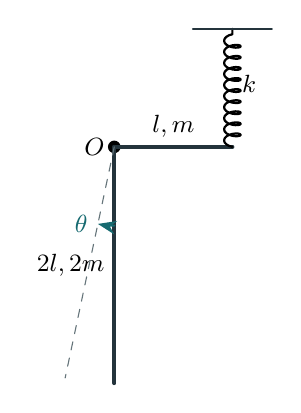
\begin{tikzpicture}[line cap=round,line join=round,spring/.style={decorate,decoration={coil,aspect=.45,segment length=4pt,amplitude=3pt},thick}]\fill (0,0) circle (.08);\node[left] at (0,0) {$O$};\draw[object,line width=1.5pt] (0,0)--(1.5,0);\draw[object,line width=1.5pt] (0,0)--(0,-3);\draw[spring] (1.5,0)--(1.5,1.5);\draw[object] (1,1.5)--(2,1.5);\node[right] at (1.5,.8) {$k$};\node[above] at (.75,0) {$l,m$};\node[left] at (0,-1.5) {$2l,2m$};\draw[guide] (0,0)--(-.623735073,-2.934442802);\draw[motion] (0,-1) arc[start angle=-90,end angle=-102,radius=1] node[left] {$\theta$};\end{tikzpicture}\figcaption{图 7.6}\end{minipage}\end{center}

\Needspace{18\baselineskip}\subsection*{解答}

\begin{center}\begin{minipage}{\linewidth}\centering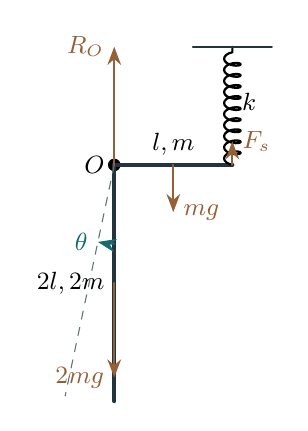
\begin{tikzpicture}[line cap=round,line join=round,spring/.style={decorate,decoration={coil,aspect=.45,segment length=4pt,amplitude=3pt},thick}]\fill (0,0) circle (.08);\node[left] at (0,0) {$O$};\draw[object,line width=1.5pt] (0,0)--(1.5,0);\draw[object,line width=1.5pt] (0,0)--(0,-3);\draw[spring] (1.5,0)--(1.5,1.5);\draw[object] (1,1.5)--(2,1.5);\node[right] at (1.5,.8) {$k$};\node[above] at (.75,0) {$l,m$};\node[left] at (0,-1.5) {$2l,2m$};\draw[guide] (0,0)--(-.623735073,-2.934442802);\draw[motion] (0,-1) arc[start angle=-90,end angle=-102,radius=1] node[left] {$\theta$};\draw[force] (1.5,0)--(1.5,.3)node[right]{$F_s$};\draw[force] (.75,0)--(.75,-.6) node[right] {$mg$};\draw[force] (0,-1.5)--(0,-2.7) node[left] {$2mg$};\draw[force](0,0)--(0,1.5)node[left]{$R_O$};\end{tikzpicture}\figcaption{解图 7.6A}\end{minipage}\end{center}
以顺时针微转角 $\theta$ 为正。平衡时水平杆端点受弹簧向上的力，抵消该臂重力矩：
\[kx_0l=mg\frac l2,\qquad x_0=\frac{mg}{2k}.\]
转动后，水平臂端点向下位移 $x=l\sin\theta=l\theta+O(\theta^3)$；水平位移为二阶，弹簧方向偏离竖直也只产生二阶及更高修正。到一阶时，合矩为
\[\begin{aligned}
\tau&=mg\frac l2\cos\theta-k(x_0+x)l\cos\theta-2mgl\sin\theta+O(\theta^3)\\
&=-(kl^2+2mgl)\theta+O(\theta^3).
\end{aligned}\]
\Needspace{11\baselineskip}解图7.6A中竖直长臂的质心距 $O$ 为 $l$，故其重力回复矩为 $-2mgl\theta$，其力臂从轴量至长臂中点。两臂的转动惯量相加：
\[I_O=\frac13ml^2+\frac13(2m)(2l)^2=3ml^2.\]
于是
\[\ddot\theta+\frac{kl+2mg}{3ml}\theta=0,\qquad
\boxed{T=2\pi\sqrt{\frac{3ml}{kl+2mg}}.}\]
在同一平衡附近展开势能，也能求出角度刚度。令平衡时势能为零，短臂质心向下移动$(l/2)\sin\theta$，长臂质心升高$l(1-\cos\theta)$，弹簧额外伸长在所保留阶次为$l\sin\theta$。因此
\[\begin{aligned}
\Delta U={}&\frac k2[(x_0+l\sin\theta)^2-x_0^2]
-\frac{mgl}{2}\sin\theta+2mgl(1-\cos\theta)+O(\theta^4)\\
={}&\frac12kl^2\sin^2\theta+2mgl(1-\cos\theta)+O(\theta^4)
\simeq\frac12(kl^2+2mgl)\theta^2.
\end{aligned}\]
第二行使用了$kx_0=mg/2$，显式显示预拉力的一次势能项与短臂重力项相消。再除以转动惯量$3ml^2$，得到与力矩法相同的$\omega^2$。

小角近似应取 $\sin\theta\simeq\theta$；若直接令它为零，会删去竖直臂的有效回复矩。弹簧静态预拉力与短臂重力的常数矩相抵，额外伸长和长臂重力共同决定频率。
\subsubsection*{固定弹簧的实际几何及近似阶次}
解图7.6B以$O$为原点，向右、向上为坐标正向，
顺时针$\theta>0$。短臂端点和弹簧固定点分别为
\[
A=(l\cos\theta,-l\sin\theta),\qquad S=(l,H),
\]
其中$H>0$是平衡时的实际弹簧长度。
端点向下位移$x=l\sin\theta$，水平位移$l(\cos\theta-1)$从二阶开始。
真实弹簧长度由两点距离确定：
\[
\ell_s=\sqrt{l^2(1-\cos\theta)^2+(H+l\sin\theta)^2}
=\sqrt{H^2+2Hl\sin\theta+2l^2(1-\cos\theta)}.
\]
其相对平衡长度的变化为
\[
\delta\ell=\ell_s-H
=l\sin\theta+\frac{l^2}{8H}\theta^4+O(\theta^5).
\]
因此求一阶力矩或二阶势能时，可用$l\sin\theta$替代真实伸长变化；
计算有限角度运动或高阶频率修正时，须恢复完整长度。
弹簧方向偏转从$\theta^2$开始，配合端点高度的一阶变化，
对力矩的修正从三阶开始，不改变本题的线性周期。

\begin{center}\begin{minipage}{\linewidth}\centering
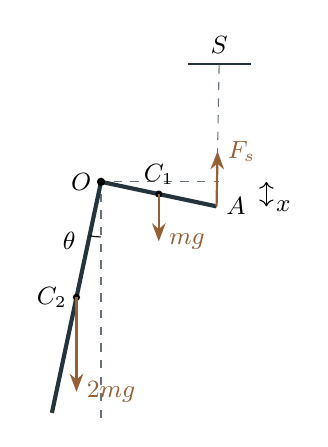
\begin{tikzpicture}[font=\small]
\coordinate(O)at(0,0);\coordinate(A)at(1.467221401,-.311867536);\coordinate(B)at(-.623735073,-2.934442802);\coordinate(S)at(1.5,1.5);
\draw[guide](0,-3)--(O)--(1.5,0);\draw[object,line width=1.5pt](A)--(O)--(B);
\draw[guide](A)--(S);\draw[object](1.1,1.5)--(1.9,1.5);
\fill(O)circle(1.5pt)node[left]{$O$};\node[right]at(A){$A$};\node[above]at(S){$S$};
\fill(.733610700,-.155933768)circle(1.3pt)node[above]{$C_1$};
\fill(-.311867536,-1.467221401)circle(1.3pt)node[left]{$C_2$};
\draw[force](.733610700,-.155933768)--++(0,-.6)node[right]{$mg$};
\draw[force](-.311867536,-1.467221401)--++(0,-1.2)node[right]{$2mg$};
\draw[force](A)--++(.012661668,.699885478)node[right]{$F_s$};
\draw[<->](2.1,0)--(2.1,-.311867536)node[right]{$x$};
\draw(0,-.7)arc(-90:-102:.7);\node[left]at(-.2,-.75){$\theta$};
\end{tikzpicture}
\figcaption{解图7.6B\quad 示例$\theta=12^\circ$；两臂长度不变，弹簧方向由固定点$S$与活动端$A$确定。}
\end{minipage}\end{center}

\subsubsection*{由真实势能求二阶回复系数}
两臂质心分别在$A/2$和长臂中点，
短臂重力势变化为$-mgl\sin\theta/2$，
长臂重力势变化为$2mgl(1-\cos\theta)$。
把真实伸长$\delta\ell$代入弹簧势能，
\[
\Delta U=\frac k2[(x_0+\delta\ell)^2-x_0^2]
-\frac{mgl}{2}\sin\theta+2mgl(1-\cos\theta).
\]
到足够确定二次项的精度，先展开平方：
\[
\Delta U=
\left(kx_0-\frac{mg}{2}\right)l\sin\theta
+\frac12kl^2\sin^2\theta+2mgl(1-\cos\theta)+O(\theta^4).
\]
括号由静态平衡为零，余下
\[
\Delta U=\frac12(kl^2+2mgl)\theta^2+O(\theta^4),
\qquad \tau=-\frac{\dd U}{\dd\theta}
=-(kl^2+2mgl)\theta+O(\theta^3).
\]
短臂重力的低阶项被预载抵消，长臂重力的二阶势能仍为$mgl\theta^2$，
所以它对角度刚度的贡献是$2mgl$。

惯量可按两个独立杆端积分，
\[
I_1=\frac ml\int_0^l r^2\dd r=\frac13ml^2,
\qquad I_2=\frac{2m}{2l}\int_0^{2l}r^2\dd r=\frac83ml^2.
\]
相加为$3ml^2$，再与角度刚度相除，
\[
\omega^2=\frac{kl^2+2mgl}{3ml^2}
=\frac{k}{3m}+\frac{2g}{3l}.
\]
两项量纲均为$1/\mathrm s^2$；质量、惯量或刚度任一处漏长臂，都会破坏这一分解。
若改变$k$或杆质量后仍使用此式，须同时保持题设的水平、下垂平衡构型，
相应调整预伸长；固定自然长和固定点而任意改参数时，平衡位置一般会改变。


\Needspace{18\baselineskip}

\pdfbookmark[2]{第 7 题 有质量弹簧振子的等效质量修正}{q7}

\section*{第 7 题\quad 有质量弹簧振子的等效质量修正}

\tagline{M-07-07}

如图7.7,弹簧振子中的小球质量为\(M\),弹簧的劲度系数为\(k\),弹簧的质量不可忽略,设为
\(m\),假定弹簧的质量分布均匀,忽略摩擦力.试求振动周期.

先采用长波、同相的近似运动形状，说明等效质量结果的适用条件。

\begin{center}\begin{minipage}{\linewidth}\centering\begin{tikzpicture}[font=\small,line cap=round,spring/.style={decorate,decoration={coil,aspect=.45,segment length=4pt,amplitude=3pt},thick}]
\draw[object](0,-.5)--(0,2.4);\draw[spring](0,2)--(4,2);\draw[object,dashed](4,1.7)rectangle(4.7,2.3);\node at(4.35,2){$M$};
\draw[spring](0,0)--(4.7,0);\draw[object,fill=white](4.7,-.3)rectangle(5.4,.3);\node at(5.05,0){$M$};
\draw[guide](4,-.8)--(4,2.3);\draw[<->](0,2.75)--(4,2.75)node[midway,above]{$L$};
\draw[motion](4,-.8)--(4.7,-.8)node[midway,below]{$u(L,t)$};
\draw[axis](0,1.1)--(4.35,1.1)node[right]{材料坐标$x$};\node[below]at(0,1.1){$0$};\node[below]at(4,1.1){$L$};
\node[right]at(5,2){未形变参考};\node[right]at(5.6,0){瞬时位置};\node[above]at(2,.3){$m,\ k$};
\end{tikzpicture}\figcaption{图 7.7}\end{minipage}\end{center}

\Needspace{18\baselineskip}\subsection*{解答}

\begin{center}\begin{minipage}{\linewidth}\centering\begin{tikzpicture}[font=\small,spring/.style={decorate,decoration={coil,aspect=.45,segment length=4pt,amplitude=3pt},thick}]
\draw[object](0,-.4)--(0,2.3);\draw[spring](0,1.8)--(4,1.8);
\draw[object,dashed](4,1.5)rectangle(4.7,2.1);\node at(4.35,1.8){$M$};
\draw[spring](0,0)--(5,0);\draw[object,fill=white](5,-.3)rectangle(5.7,.3);\node at(5.35,0){$M$};
\draw[guide](4,-.8)--(4,2.2);
\draw[<->](0,2.65)--(4,2.65)node[midway,above]{$l_0$};
\draw[<->](4,-.8)--(5,-.8)node[midway,below]{$x$};
\node[right]at(5,1.8){平衡};\node[left]at(0,0){$m,k$};
\foreach \p/\v in {1.25/.3,2.5/.6,3.75/.9,5/1.2}{\draw[guide](\p,.1)--(\p,.55);\draw[motion](\p,.55)--++(\v,0);}
\node at(2.7,1.05){$v(\xi)=\xi\dot x/l_0$};
\node[below]at(2,-.8){示意$x=l_0/4,\ \dot x>0$};
\end{tikzpicture}\figcaption{解图 7.7A\quad 固定端速度为零，材料坐标$\xi$的质元速度按$\xi/l_0$递增；细虚线从质元引出速度箭头。}\end{minipage}\end{center}
设弹簧原长 $l_0$，从固定端沿原长坐标 $\xi$ 量取质元。均匀线密度给 $\dd m=(m/l_0)\dd\xi$。采用长波近似的线性位移形状，
\[u(\xi,t)=\frac{\xi}{l_0}x(t),\qquad
\dot u=\frac{\xi}{l_0}\dot x.\]
解图7.7A的速度从固定端零值线性增到末端 $\dot x$。弹簧动能需沿全长积分：
\[\begin{aligned}
K_s&=\int_0^{l_0}\frac12\dot u^2\dd m
=\frac{m\dot x^2}{2l_0^3}\int_0^{l_0}\xi^2\dd\xi
=\frac16m\dot x^2,\\
K&=\frac12\left(M+\frac m3\right)\dot x^2.
\end{aligned}\]
线性位移形状意味着各段具有相同应变$\partial u/\partial\xi=x/l_0$。以整根弹簧静态刚度$k$写其等效轴向弹性系数为$kl_0$，则
\[U_s=\frac12kl_0\int_0^{l_0}
\left(\frac{\partial u}{\partial\xi}\right)^2\dd\xi
=\frac12kx^2.\]
动能与应变能都采用这一线性位移形状，分别由其时间导数和空间导数积分。

弹性势能仍为 $kx^2/2$，总能量为
\[E=\frac12\left(M+\frac m3\right)\dot x^2+\frac12kx^2.\]
求导并连续延伸到 $\dot x=0$ 的转折点，得
\[\left(M+\frac m3\right)\ddot x+kx=0,\qquad
\boxed{T\simeq2\pi\sqrt{\frac{M+m/3}{k}}.}\]
等效质量 $m/3$ 来自速度平方积分，其中各质元均参与运动。用平均速度会给$m/4$，相差的部分是相对质心动能。该线性振型式适用于低频长波近似，质量比可比时由连续本征方程确定频率。
\Needspace{12\baselineskip}若保留连续弹簧波动，波速 $c=l_0\sqrt{k/m}$；取 $u\propto\sin(\alpha\xi/l_0)$，固定端和末端质量条件给
\[\alpha\tan\alpha=\frac mM,\quad 0<\alpha<\frac\pi2,
\qquad\omega=\alpha\sqrt{k/m}.\]
当 $m/M\ll1$，$\tan\alpha=\alpha+\alpha^3/3+\cdots$，故
\[\alpha^2=\frac mM-\frac13\left(\frac mM\right)^2+\cdots,
\quad\omega^2=\frac kM\left(1-\frac m{3M}+\cdots\right),\]
与等效质量公式的一阶修正一致。
\subsubsection*{材料坐标、位移形状与三分之一的积分}
解图7.7A中$\xi$从固定端沿未伸长弹簧量起，
$l_0$是原长，$x(t)$只是活动端相对平衡的位移。
示意取$x=l_0/4$时，原坐标$\xi$的质元位于
$\xi+u=\xi(1+x/l_0)$，$\xi$标记未伸长时的材料位置，当前空间位置还加上该质元的位移。
线性形状满足$u(0,t)=0,u(l_0,t)=x(t)$，
对时间求导给每一质元的实际轴向速度。
把质元质量和速度同时代入，完整的动能微元为
\[
\dd K_s=\frac12\frac m{l_0}\dd\xi
\left(\frac\xi{l_0}\dot x\right)^2
=\frac{m\dot x^2}{2l_0^3}\xi^2\dd\xi.
\]
沿全长积分，
\[
K_s=\frac{m\dot x^2}{2l_0^3}
\left[\frac{\xi^3}{3}\right]_0^{l_0}
=\frac16m\dot x^2=\frac12\frac m3\dot x^2.
\]
与末端质量动能$M\dot x^2/2$相加，才得到$M+m/3$。
全弹簧的平均速度虽为$\dot x/2$，
但动能由速度平方的平均决定：
\[
\langle v\rangle=\frac{\dot x}{l_0^2}\int_0^{l_0}\xi\dd\xi=\frac{\dot x}{2},
\qquad
\langle v^2\rangle=\frac{\dot x^2}{l_0^3}\int_0^{l_0}\xi^2\dd\xi=\frac{\dot x^2}{3}.
\]
方差$\langle v^2\rangle-\langle v\rangle^2=\dot x^2/12$对应弹簧相对自身质心的运动动能。

由同一线性形状算出的应变能为$kx^2/2$，
能量导数逐项为
\[
\dot E=(M+m/3)\dot x\ddot x+kx\dot x
=\dot x[(M+m/3)\ddot x+kx]=0.
\]
在运动段得到方程，转折点取连续极限。
因采用近似运动形状，求得的周期须保留近似号。

\subsubsection*{连续模型中的固定端与活动端条件}
在连续弹簧模型中，取均匀线密度$\lambda=m/l_0$，
轴向弹性系数为$kl_0$。
小段两端的弹力差给
\[
\lambda\dd\xi\,u_{tt}=kl_0 u_{\xi\xi}\dd\xi,
\quad u_{tt}=c^2u_{\xi\xi},\quad
c=l_0\sqrt{k/m}.
\]
固定端要求$u(0,t)=0$。
另一端连接质量$M$，以该端质量的牛顿方程给端条件：
\[
M u_{tt}(l_0,t)=-kl_0 u_\xi(l_0,t).
\]
取同相基频$u=C\sin(\alpha\xi/l_0)\cos\omega t$，
波动方程先给$\omega=\alpha c/l_0$。
再代端质量条件，逐项消去公共振幅，
\[
M\omega^2\sin\alpha=k\alpha\cos\alpha,
\quad \frac{M\alpha^2}{m}\sin\alpha=\alpha\cos\alpha,
\quad \alpha\tan\alpha=\frac mM.
\]
基频根在$0<\alpha<\pi/2$内，此处$\alpha\tan\alpha$严格递增，
所以正根唯一。更高的根给出不同的振型和相应频率，动能与应变能按各振型分别积分。

\subsubsection*{基频随质量比的变化与试探振型的刚度}
令$\varepsilon=m/M$、$y=\alpha^2$，
把正切展开代入边界式，
\[
\varepsilon=y+\frac{y^2}{3}+\frac{2y^3}{15}+O(y^4).
\]
设$y=\varepsilon+a\varepsilon^2+b\varepsilon^3+\cdots$，
比较同次幂得到
\[
a+\frac13=0,\qquad b+\frac{2a}{3}+\frac{2}{15}=0,
\quad y=\varepsilon-\frac{\varepsilon^2}{3}+\frac{4\varepsilon^3}{45}+\cdots.
\]
因此精确基频的展开为
\[
\omega^2=\frac kM\left(1-\frac\varepsilon3+\frac{4\varepsilon^2}{45}+\cdots\right),
\]
而$k/(M+m/3)$给二阶系数$1/9$，只在一阶修正上相同。
当$m=M$时，数值根$\alpha=0.860333589\cdots$，
线性形状估计$\omega/\sqrt{k/m}=\sqrt{3/4}=0.866025404\cdots$，
频率约高$0.662\%$、周期约低$0.657\%$。
当$M\to0$时，连续模型为自由端$\alpha\to\pi/2$，
等效质量公式却给$\sqrt3$，说明此时线性形状失去依据。

若改用试探形状$u=x(\xi/l_0)^p$，$p>1/2$，
分别用该形状的速度和轴向应变积分，得到
\[
m_{\rm eff}=\frac m{2p+1},\qquad
k_{\rm eff}=\frac{kp^2}{2p-1},\qquad
\omega_{\rm trial}^2=
\frac{kp^2}{(2p-1)[M+m/(2p+1)]}.
\]
形状指数同时改变质元的速度分布和应变分布，因此等效质量与刚度都随指数变化。


\Needspace{18\baselineskip}

\pdfbookmark[2]{第 8 题 小孔圆周运动与悬挂重物的耦合振动}{q8}

\section*{第 8 题\quad 小孔圆周运动与悬挂重物的耦合振动}

\tagline{M-07-08}

如图,一不可伸长的细线穿过光滑桌面上的小孔,一端系质量为\(m\)的小球,另一端系质

量为 \(M\) 的重物．小球在桌面上以角速度 \(\omega_{0}\)
作匀速圆周运动，重物静止不动．若重物受到竖直向上或向下的扰动．试证明，重物将作上、下的简谐振动，并求振动圆频率．

扰动位移远小于原圆轨道半径，细线始终绷紧。

\begin{center}\begin{minipage}{\linewidth}\centering\begin{tikzpicture}[font=\small]
\begin{scope}[shift={(-2,0)}]
\draw[guide](0,0)circle(1.4);\fill(0,0)circle(1.2pt)node[below left]{$O$};
\draw[object](0,0)--(1.4,0);\fill[accent](1.4,0)circle(1.8pt)node[right]{$m$};
\draw[motion](1.315569670,.478828201)arc(20:85:1.4);\node[above]at(1.5,1){$\omega_0$};
\node[below]at(.7,0){$r_0$};\node at(0,2.1){俯视：未扰动圆轨道};
\end{scope}
\begin{scope}[shift={(3,0)}]
\draw[object](-1.6,0)--(1.9,0);\draw[object](0,0)--(0,-1.8);\draw[object](0,0)--(1.4,0);
\fill[accent](1.4,0)circle(1.8pt)node[above right]{$m$};\fill(0,0)circle(1pt)node[above left]{$O$};
\fill[accent](0,-1.8)circle(2.3pt)node[left]{$M$};
\draw[<->](0,.65)--(1.4,.65)node[midway,above]{$r$};
\draw[<->](-.55,0)--(-.55,-1.8)node[midway,left]{$l-r$};
\node at(.4,2.1){侧视：绳长约束};
\end{scope}
\end{tikzpicture}\figcaption{图 7.8}\end{minipage}\end{center}

\Needspace{18\baselineskip}\subsection*{解答}

\begin{center}\begin{minipage}{\linewidth}\centering\begin{tikzpicture}[font=\small]
\begin{scope}[shift={(-2,0)}]
\draw[guide](0,0)circle(1.6);\fill(0,0)circle(1.2pt)node[below left]{$O$};
\draw[object](0,0)--(1.4,0);\fill[accent](1.4,0)circle(1.8pt)node[right]{$m$};
\draw[force](1.4,0)--(.402915452,0);\draw[motion](1.4,0)--(1.4,.85);\node[above]at(1.5,1){$r\dot\varphi$};
\node[below]at(.7,0){$r$};\node at(0,2.1){俯视：虚线为平衡圆};
\end{scope}
\begin{scope}[shift={(3,0)}]
\draw[object](-1.6,0)--(1.9,0);\draw[object](0,0)--(0,-1.8);\draw[object](0,0)--(1.4,0);
\fill[accent](1.4,0)circle(1.8pt)node[above right]{$m$};\fill(0,0)circle(1pt)node[above left]{$O$};
\fill[accent](0,-1.8)circle(2.3pt)node[left]{$M$};
\draw[<->](0,1.15)--(1.4,1.15)node[midway,above]{$r$};
\draw[<->](-.55,0)--(-.55,-1.8)node[midway,left]{$l-r$};
\draw[force](1.4,0)--(.402915452,0)node[midway,below]{$T$};
\draw[force](0,-1.8)--(0,-.802915452)node[right]{$T$};
\draw[force](0,-1.8)--(0,-2.6)node[right]{$Mg$};
\draw[force](1.4,0)--(1.4,.8)node[right]{$N$};
\draw[force](1.4,0)--(1.4,-.8)node[right]{$mg$};
\node at(.4,2.1){侧视：张力随运动变化};
\end{scope}
\end{tikzpicture}\figcaption{解图 7.8A\quad 受力示例取$M=m,r=7r_0/8$，此时$T>Mg$；俯视的上箭头为切向速度。}\end{minipage}\end{center}
令桌面小球径向距离为 $r$，细线全长为 $l$；悬重距桌面向下的长度为 $z=l-r$。未扰动时
\[T_0=Mg=mr_0\omega_0^2,\qquad r_0=\frac{Mg}{m\omega_0^2}.\]
扰动不对小球施加绕孔的力矩，角动量 $L=mr^2\dot\varphi=mr_0^2\omega_0$ 保持不变。两个运动方程为
\[Mg-T=M\ddot z=-M\ddot r,
\qquad m(\ddot r-r\dot\varphi^2)=-T.\]
先由悬重方程求$T=Mg+M\ddot r$，再代入桌面小球式，得到
\[(M+m)\ddot r=mr\dot\varphi^2-Mg.\]
半径改变时两物体都在加速，故径向惯性是$M+m$；切向速度则由角动量守恒变为$\dot\varphi=L/(mr^2)$，所以离心项随$r^{-3}$变化。解图7.8A中的两段运动正是通过不可伸长绳约束连接起来。

消去张力和角速度：
\[(M+m)\ddot r-\frac{L^2}{mr^3}+Mg=0.\]
解图7.8A中半径增加对应悬重上升，$\delta=r-r_0$ 与悬重向下位移符号相反。对 $|\delta|\ll r_0$ 展开，
\[\frac1{r^3}=\frac1{r_0^3}\left(1-\frac{3\delta}{r_0}
+O(\delta^2/r_0^2)\right).\]
\Needspace{13\baselineskip}平衡项 $L^2/(mr_0^3)=Mg$ 相消，剩下
\[(M+m)\ddot\delta+\frac{3Mg}{r_0}\delta=0,\qquad
\boxed{\Omega=\sqrt{\frac{3Mg}{(M+m)r_0}}
=\omega_0\sqrt{\frac{3m}{M+m}}.}\]
给定初位移与速度时 $\delta(t)=\delta_0\cos\Omega t+
\dot\delta_0\sin\Omega t/\Omega$；悬重位移为其负值。此处是小振动，并非任意大扰动都严格简谐。
能量另一求法：
\[E=\frac12(M+m)\dot r^2+\frac{L^2}{2mr^2}-Mg(l-r).\]
第一项包括两物体的径向、竖直动能，第二项是小球切向动能。用有效势对$r$求梯度，或将总能量对时间求导，均还原上面的非线性方程；有效势能二阶导数为 $3Mg/r_0$。
\subsubsection*{两种位移的反号和张力消元全步}
解图7.8A分别给俯视和侧视。
桌面小球沿径向向外为$r$正向，悬重向下的坐标为$z=l-r$，
因此$\dot z=-\dot r$、$\ddot z=-\ddot r$。
圆运动初态的两条平衡式是$T_0=Mg$与$T_0=mr_0\omega_0^2$，
所以先有$r_0=Mg/(m\omega_0^2)$，还须$0<r_0<l$使两段绳长都为正。

扰动后悬重的方程给
\[
Mg-T=-M\ddot r,\qquad T=Mg+M\ddot r.
\]
桌面小球的极坐标径向加速度是$\ddot r-r\dot\varphi^2$，
并非单独的$-r\omega_0^2$，故
\[
m\ddot r-mr\dot\varphi^2=-T=-Mg-M\ddot r.
\]
把两个含$\ddot r$项移到一起，
$(M+m)\ddot r=mr\dot\varphi^2-Mg$。
张力沿孔到小球的连线，对孔的竖直轴力矩为零；
竖直重力和支持力也不给这根轴力矩。
所以绕孔角动量守恒，
\[
L=mr^2\dot\varphi=mr_0^2\omega_0,
\quad mr\dot\varphi^2=\frac{L^2}{mr^3}.
\]
将角动量表达式代入径向方程，得到只含$r$的非线性方程。
悬重不再静止时张力一般不等于$Mg$；半径改变时角速度也不等于$\omega_0$。

\subsubsection*{负三次幂展开、回复项与两个初值}
令$r=r_0+\delta$，将倒数的负三次幂完整写成
\[
\frac1{r^3}=\frac1{r_0^3}
\left(1+\frac\delta{r_0}\right)^{-3}
=\frac1{r_0^3}\left[1-\frac{3\delta}{r_0}
+\frac{6\delta^2}{r_0^2}+O(\delta^3/r_0^3)\right].
\]
保留一阶并代回，
\[
(M+m)\ddot\delta-
\frac{L^2}{mr_0^3}
+\frac{3L^2}{mr_0^4}\delta+Mg=0.
\]
用$L^2/(mr_0^3)=Mg$消去常数项，
剩下的刚度为$3Mg/r_0$，除以参与运动的总惯性$M+m$才得到$\Omega^2$。
再用$r_0=Mg/(m\omega_0^2)$逐项替换，
\[
\Omega^2=\frac{3Mg}{(M+m)r_0}
=\frac{3m\omega_0^2}{M+m},
\qquad \Omega=\omega_0\sqrt{\frac{3m}{M+m}}.
\]
$\Omega^2$含$\omega_0^2$，开方后$\Omega$与$\omega_0$同为角频率。
初始给悬重向下位移$\eta_0$和向下速度$w_0$时，
对应$\delta_0=-\eta_0$、$\dot\delta_0=-w_0$，
所以悬重位移直接为
\[
\eta(t)=\eta_0\cos\Omega t+\frac{w_0}{\Omega}\sin\Omega t.
\]
向上扰动只改变这两个有符号初值，不改变线性频率。

\subsubsection*{机械能各项与有效势能曲率}
悬重竖直动能为$M\dot r^2/2$，
桌面小球的径向、切向动能分别为$m\dot r^2/2$与$mr^2\dot\varphi^2/2$。
用角动量守恒消去切向速度，再以桌面为重力势能零点，
\[
E=\frac12M\dot r^2+\frac12m\dot r^2
+\frac{L^2}{2mr^2}-Mg(l-r).
\]
对时间逐项求导，
\[
0=\dot E=(M+m)\dot r\ddot r
-\frac{L^2}{mr^3}\dot r+Mg\dot r.
\]
在运动段约去$\dot r$并延伸到转折点，恢复同一非线性方程。
忽略常数$-Mgl$的有效势为
\[
U(r)=\frac{L^2}{2mr^2}+Mgr,\quad
U'=-\frac{L^2}{mr^3}+Mg,\quad
U''=\frac{3L^2}{mr^4}>0.
\]
平衡是唯一极小，$U''(r_0)=3Mg/r_0$。
令$q=r/r_0$，势能可归一化为$U/(Mgr_0)=1/(2q^2)+q$。
\begin{center}\begin{minipage}{\linewidth}\centering
\begin{tikzpicture}[font=\small,x=3cm,y=1.6cm]
\draw[axis](.4,1.3)--(2.25,1.3)node[right]{$q=r/r_0$};
\draw[axis](.4,1.3)--(.4,3.2)node[above]{$U/(Mgr_0)$};
\draw[traj,domain=.45:2.1,samples=101]plot(\x,{1/(2*\x^2)+\x});
\draw[guide,domain=.7:1.3,samples=51]plot(\x,{1.5+1.5*(\x-1)^2});
\draw[guide](1,1.3)--(1,1.5);\fill(1,1.5)circle(1.2pt);
\node[below]at(1,1.3){$1$};\node[left]at(.4,1.5){$3/2$};
\node[above]at(1.45,2.4){实线：完整势能};\node[above]at(1.45,2.1){虚线：局部二次项};
\end{tikzpicture}
\figcaption{解图7.8B\quad 固定角动量的有效势；局部曲率给小振动频率，远离极小后不再是抛物线。}
\end{minipage}\end{center}
进一步展开有
\[
U-U(r_0)=\frac{3Mg}{2r_0}\delta^2
-\frac{2Mg}{r_0^2}\delta^3
+\frac{5Mg}{2r_0^3}\delta^4+\cdots.
\]
三次及更高项解释了有限幅运动一般不严格简谐；
题设的上下简谐结论限于小扰动。

\subsubsection*{绳长、张力及改变质量时固定的参数}
小振动振幅为$A=\sqrt{\delta_0^2+(\dot\delta_0/\Omega)^2}$，
须$A\ll r_0$，且$A<\min(r_0,l-r_0)$，
使桌面半径和孔下长度在全段都为正。
用完整非线性方程反代张力，
\[
T=Mg+\frac M{M+m}\left(\frac{L^2}{mr^3}-Mg\right)
=\frac{Mm}{M+m}g+\frac{ML^2}{m(M+m)r^3}>0
\quad(r>0).
\]
绳长约束要求 $0<r<l$，完整张力式的两项都为正，所以绳保持绷紧。小扰动区间 $|\delta|\ll r_0$ 内，将张力保留到一阶得 $T\simeq Mg-M\Omega^2\delta$，能直接读出张力随半径增大而减小。计算幅度较大的运动时，使用上面的完整张力式。

改变质量时，频率的变化取决于同时保持的圆运动参数。
固定$r_0$而改变$M$，需同时改变平衡圆角速度，
$\Omega^2=3Mg/[(M+m)r_0]$随$M$增大并趋于$3g/r_0$。
若固定$\omega_0$，则$r_0$随$M$增加，
$\Omega=\omega_0\sqrt{3m/(M+m)}$反而减小，
还须检查增长的$r_0$没有超过绳长$l$。


\Needspace{18\baselineskip}

\pdfbookmark[2]{第 9 题 旋转平板上弹簧质点的相对运动}{q9}

\section*{第 9 题\quad 旋转平板上弹簧质点的相对运动}

\tagline{M-07-09}

如图7.9,光滑的水平平板绕铅垂轴Oz逆时针作匀角速转动,角速度为\(\omega\).在板面上,一质量可略、原长为\(l\)、劲度系数为\(k\)的弹簧一端固定在O点,另一端系一质量为\(m\)的小球.开始时小球位于\((x_0,0)\),初速度为\((v_0,0)\).试求小球相对平板的运动方程\(x=x(t)\),\(y=y(t)\).

给出的初速度为相对地面的速度；平板坐标轴在初始时与地面轴重合。小球运动限于弹簧长度保持正值的区间。

\begin{center}\begin{minipage}{\linewidth}\centering\begin{tikzpicture}[font=\small,spring/.style={decorate,decoration={coil,aspect=.45,segment length=4pt,amplitude=3pt},thick}]
\draw[guide](0,0)circle(2.2);\draw[axis](-.3,0)--(2.9,0)node[right]{$X=x$};
\draw[axis](0,-.3)--(0,2.8)node[above]{$Y=y$（初始）};
\draw[spring](0,0)--(1.7,0);\fill(0,0)circle(1pt)node[below left]{$O$};
\fill[accent](1.7,0)circle(2pt)node[above]{$m$};
\draw[motion](1.230224387,1.82388266)arc(56:105:2.2)node[left]{$\omega$};
\draw[motion](1.7,-.4)--(2.5,-.4)node[right]{$v_0$（地面）};
\draw[<->](0,-.85)--(1.7,-.85)node[midway,below]{$x_0$};
\end{tikzpicture}\figcaption{图 7.9}\end{minipage}\end{center}

\Needspace{18\baselineskip}\subsection*{解答}

\begin{center}\begin{minipage}{\linewidth}\centering\begin{tikzpicture}[font=\small]
\fill(0,0)circle(1pt)node[below left]{$O$};\draw[object](0,0)--(2,0);
\fill[accent](2,0)circle(2pt)node[below left]{$P$};
\draw[axis](2,0)--(3.4,0)node[right]{$\hat{\boldsymbol r}$};
\draw[axis](2,0)--(2,1.5)node[above]{$\hat{\boldsymbol\theta}$};
\draw[motion](2,0)--(2.8,0)node[above]{$\boldsymbol v_{\text{地}}$};
\draw[motion](2,0)--(2.8,-1.1)node[midway,below left]{$\boldsymbol v'$};
\draw[motion](2.8,-1.1)--(2.8,0)node[midway,right]{$\boldsymbol\omega\times\boldsymbol r$};
\draw[force](2,0)--(.9,0)node[midway,below]{$-k(r-l)\hat{\boldsymbol r}$};
\node at(1.9,-1.8){初始：$\boldsymbol v_{\text{地}}=\boldsymbol v'+\boldsymbol\omega\times\boldsymbol r,\quad L_z=0$};
\end{tikzpicture}\figcaption{解图 7.9A}\end{minipage}\end{center}
用地面惯性系先确定运动，再变换到逆时针转动的平板坐标。题给初速度是地面速度，初始位置和速度共线，弹簧力也沿半径，所以关于 $O$ 的角动量为零且保持零值。小球沿初始地面 $X$ 轴往复运动，限于 $r>0$ 的区间：
\[m\ddot r=-k(r-l),\qquad\Omega_0=\sqrt{k/m}.\]
由 $r(0)=x_0$、$\dot r(0)=v_0$，直接解得
\[r(t)=l+(x_0-l)\cos\Omega_0t+\frac{v_0}{\Omega_0}\sin\Omega_0t.\]
平板轴转过 $\omega t$，同一地面方向在板面坐标中的角度为 $-\omega t$，故
\[\boxed{\begin{aligned}
x(t)&=r(t)\cos\omega t,\\
y(t)&=-r(t)\sin\omega t.
\end{aligned}}\]
若用振幅相位形式，$A=\sqrt{(x_0-l)^2+(v_0/\Omega_0)^2}$，$\phi=\operatorname{atan2}(-v_0/\Omega_0,x_0-l)$，则 $r=l+A\cos(\Omega_0t+\phi)$。要求 $l>A$ 可以保证整个周期中弹簧长度为正；若触及 $O$，中心力方向和弹簧几何须重新处理。
将同一运动写入转动系的分量方程。解图7.9A标出 $\hat{\boldsymbol r}$、$\hat{\boldsymbol\theta}$，相对速度为
\[\boldsymbol v'=\dot r\hat{\boldsymbol r}-\omega r\hat{\boldsymbol\theta},\quad
\boldsymbol\omega\times\boldsymbol v'
=\omega\dot r\hat{\boldsymbol\theta}+\omega^2r\hat{\boldsymbol r}.\]
转动系方程
\[m\boldsymbol a'=-k(r-l)\hat{\boldsymbol r}
+m\omega^2r\hat{\boldsymbol r}-2m\boldsymbol\omega\times\boldsymbol v'\]
的径向分量为 $m(\ddot r-\omega^2r)=-k(r-l)-m\omega^2r$，相消后仍为上述径向方程；切向分量两端都是 $-2m\omega\dot r$。
因此初始相对板的横向速度为 $\dot y(0)=-\omega x_0$，与平板转动方向相反。若把初速 $(v_0,0)$ 改为相对平板给定，换回地面后便有 $L=m\omega x_0^2$，相应的径向方程为
\[m\ddot r=\frac{L^2}{mr^3}-k(r-l),\qquad
\dot\theta'=\frac{L}{mr^2}-\omega.\]
此时从 $r(0)=x_0,\dot r(0)=v_0,\theta'(0)=0$ 积分，相对角速度由前一式确定，区别于 $\theta'=-\omega t$。
\subsubsection*{先变换初速度，再判断角动量}
图7.9中地面轴记为$X,Y$，板面轴记为$x,y$，初始两套轴重合。
板面以$\boldsymbol\omega=\omega\hat{\boldsymbol z}$逆时针转动，
任意时刻的速度变换为
\[
\boldsymbol v_{\text{地}}=\boldsymbol v'
+\boldsymbol\omega\times\boldsymbol r.
\]
初始位置$(x_0,0)$处的牵连速度为$(0,\omega x_0)$。
题给地面初速度$(v_0,0)$，所以解图7.9A的相对初速度须为
\[
(\dot x(0),\dot y(0))=(v_0,-\omega x_0).
\]
地面角动量的初值是$m(x_0v_Y-0v_X)=0$，
而弹力为$-k(r-l)\boldsymbol r/r$，对$O$无力矩，
故$mr^2\dot\Theta=0$。
只要$r>0$，有$\dot\Theta=0$；取初始方向$\Theta=0$，
才得到板系方位角$\theta=\Theta-\omega t=-\omega t$。
这里角度关系由零地面角动量的初值确定；平板光滑只说明没有板面摩擦。

\subsubsection*{径向初值、相位象限与坐标投影}
令$q=r-l$，由$m\ddot r=-k(r-l)$得
$\ddot q+\Omega_0^2q=0$。
写$q=C\cos\Omega_0t+D\sin\Omega_0t$，逐项代初值，
\[
C=x_0-l,\qquad \Omega_0D=v_0.
\]
与$A\cos(\Omega_0t+\phi)$比较，
\[
A\cos\phi=x_0-l,\quad -A\sin\phi=v_0/\Omega_0,
\quad A^2=(x_0-l)^2+(v_0/\Omega_0)^2.
\]
应同时由正弦、余弦定象限。
仅用一个反正切比值会漏掉相差$\pi$的相位；
$A=0$时径向运动恒定，初相位没有唯一值。

\begin{center}\begin{minipage}{\linewidth}\centering
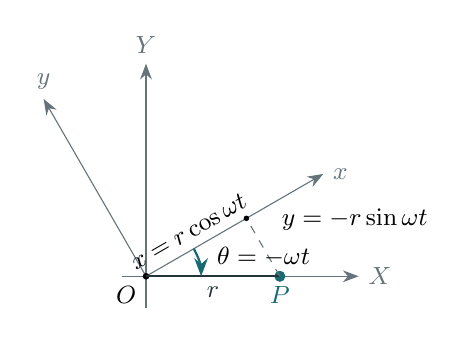
\begin{tikzpicture}[font=\small]
\draw[axis](-.3,0)--(2.7,0)node[right]{$X$};
\draw[axis](0,-.4)--(0,2.7)node[above]{$Y$};
\draw[axis](0,0)--(2.25166605,1.3)node[right]{$x$};
\draw[axis](0,0)--(-1.3,2.25166605)node[above]{$y$};
\fill(0,0)circle(1.2pt)node[below left]{$O$};
\fill[accent](1.7,0)circle(2pt)node[below]{$P$};
\draw[object](0,0)--(1.7,0)node[midway,below]{$r$};
\draw[guide](1.7,0)--(1.275,.736121593);\fill(1.275,.736121593)circle(1pt);
\draw[motion](.606217783,.35)arc(30:0:.7);
\node[right]at(.78,.25){$\theta=-\omega t$};
\node[above,rotate=30]at(.65,.375){$x=r\cos\omega t$};
\node[right]at(1.6,.72){$y=-r\sin\omega t$};
\end{tikzpicture}
\figcaption{解图7.9B\quad 地面方向$OP$不转，板面轴逆时针转；负的板面$y$坐标由垂线投影确定。}
\end{minipage}\end{center}
解图7.9B对应旋转矩阵
\[
\begin{pmatrix}x\\y\end{pmatrix}
=\begin{pmatrix}\cos\omega t&\sin\omega t\\-\sin\omega t&\cos\omega t\end{pmatrix}
\begin{pmatrix}r\\0\end{pmatrix}.
\]
分别求导，两个初速度由下式读出：
\[
\dot x=\dot r\cos\omega t-\omega r\sin\omega t,
\quad\dot y=-\dot r\sin\omega t-\omega r\cos\omega t.
\]
若$\omega/\Omega_0$为有理数，正长度运动的两个相位有公共周期，
相对轨迹可闭合；比值无理且径向振幅非零时，一般没有这样的公共周期。
$A=0$时仅余坐标旋转，相对轨迹只按坐标旋转的频率重复。

\subsubsection*{转动系的径向方程与非零角动量的初值}
取$\hat{\boldsymbol r}\times\hat{\boldsymbol\theta}=\hat{\boldsymbol z}$，
则$\hat{\boldsymbol z}\times\hat{\boldsymbol r}=\hat{\boldsymbol\theta}$、
$\hat{\boldsymbol z}\times\hat{\boldsymbol\theta}=-\hat{\boldsymbol r}$。
代$\dot\theta=-\omega$后，
\[
\boldsymbol a'=(\ddot r-\omega^2r)\hat{\boldsymbol r}
-2\omega\dot r\hat{\boldsymbol\theta},
\quad
\boldsymbol F_{\rm Cor}=-2m\omega^2r\hat{\boldsymbol r}
-2m\omega\dot r\hat{\boldsymbol\theta}.
\]
科里奥利力的径向项与离心力$m\omega^2r\hat{\boldsymbol r}$相加后，
径向净惯性力为$-m\omega^2r$。
径向方程两侧各有一项$-\omega^2r$乘质量，相消后剩下弹簧回复方程。切向两端同为$-2m\omega\dot r$。惯性项与相对加速度中的对应项相消，所得径向自然频率与$\omega$无关。

若改给板面径向初速度，地面初速度变成$(v_0,\omega x_0)$，
角动量为$m\omega x_0^2$。
其有效势为
\[
U_{\rm eff}=\frac{L^2}{2mr^2}+\frac12k(r-l)^2,
\quad E=\frac12m\dot r^2+U_{\rm eff}.
\]
在相邻转折点之间由能量取与运动方向相符的根，
\[
\dot r=\pm\sqrt{\frac2m[E-U_{\rm eff}(r)]},\qquad
\theta(t)=\int_0^t\frac{L}{mr(s)^2}\dd s-\omega t.
\]
能量式先给径向位置随时间的变化，再沿该径向运动积分角速度，得到板上的方位角。
长度正值只保证径向几何有定义；若连接只可拉不可压，
还须$r(t)\ge l$。要在$l$两侧往复使用线性弹力，需能承受拉压的理想弹簧。


\Needspace{18\baselineskip}

\pdfbookmark[2]{第 10 题 狭长湖泊湖震的整体振荡模型}{q10}

\section*{第 10 题\quad 狭长湖泊湖震的整体振荡模型}

\tagline{M-07-10}

狭长、较浅的湖泊可出现湖震，即水体的长周期整体振荡。这里采用矩形容器和平面液面的近似模型，描述水体的长波整体振荡。

我们用一只矩形容器作模型．容器的长度为\(L\)，水高为\(h\)．假定水面开始时与水平面成一小角度．水面开始振荡，振荡时水面仍保持平面，只是绕位于容器长度一半处的水平轴作振荡．

试建立水运动的模型,并求出振荡周期 \(T\) 的表达式.
初始右端液面升高\(\xi\)、左端降低\(\xi\)，从静止开始振荡。 假定
\(\xi \ll h\).

2.下面两个表显示在两种不同长度的容器中,不同深度的水

的振荡时间．以适当的方法检查你得出的公式，看它是否与实验数据很好吻合，并说明你对这种
物理模型的适用性的意见．

表 1 \(L=479 \mathrm{mm}\)

{\def\LTcaptype{none} % do not increment counter
\begin{longtable}[]{@{}ll@{}}
\toprule\noalign{}
h /mm & T /s \\
\midrule\noalign{}
\endhead
\bottomrule\noalign{}
\endlastfoot
30 & 1.78 \\
50 & 1.40 \\
69 & 1.18 \\
88 & 1.08 \\
107 & 1.00 \\
124 & 0.91 \\
142 & 0.82 \\
\end{longtable}
}

表 2 \(L=143 \mathrm{mm}\)

{\def\LTcaptype{none} % do not increment counter
\begin{longtable}[]{@{}ll@{}}
\toprule\noalign{}
$h/\mathrm{mm}$ & \(T/s\) \\
\midrule\noalign{}
\endhead
\bottomrule\noalign{}
\endlastfoot
31 & 0.52 \\
38 & 0.48 \\
58 & 0.43 \\
67 & 0.35 \\
124 & 0.28 \\
\end{longtable}
}

瑞典 Vattern 湖的北端 Bastedalen 与南端 Jonköping
分别测量了湖震时的液面变化。 该湖长度为 123 km,平均深度为 50 m.
在此情况下,时间标度应是什么?

\begin{center}\begin{minipage}{\linewidth}\centering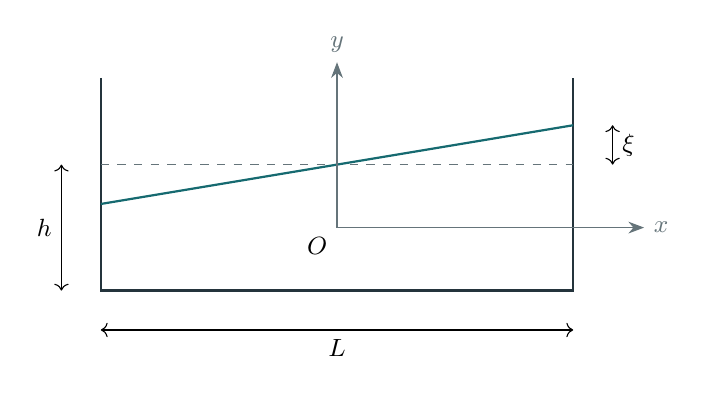
\begin{tikzpicture}[font=\small]
\draw[object](-3,1.7)--(-3,-1)--(3,-1)--(3,1.7);
\draw[guide](-3,.6)--(3,.6);\draw[traj](-3,.1)--(3,1.1);
\draw[<->](3.5,.6)--(3.5,1.1)node[midway,right]{$\xi$};
\draw[<->](-3.5,-1)--(-3.5,.6)node[midway,left]{$h$};
\draw[<->](-3,-1.5)--(3,-1.5)node[midway,below]{$L$};
\draw[axis](0,-.2)--(0,1.9)node[above]{$y$};
\draw[axis](0,-.2)--(3.9,-.2)node[right]{$x$};\node[below left]at(0,-.2){$O$};
\end{tikzpicture}\figcaption{图 7.10}\end{minipage}\end{center}
\begin{center}\begin{minipage}{.97\linewidth}\centering
\begin{tikzpicture}[x=.75cm,y=.75cm,font=\small]
\begin{scope}[yshift=4.4cm]
\draw[axis] (0,-.45)--(0,4.1) node[above]{记录读数};
\draw[axis] (0,0)--(10.6,0) node[right]{时间};
\foreach \v in {0,10,20}{\draw (0,{\v/5})--(-.1,{\v/5}) node[left]{$\v$};}
\node at (5.2,3.55){Bastedalen};
\draw[traj] plot coordinates{(0.069,3.6667) (0.1034,3.3158) (0.1379,2.693) (0.1724,2.3333) (0.2069,1.7193) (0.2414,1.1579) (0.2759,0.4561) (0.3103,0.6842) (0.3448,0.9123) (0.3793,1.1404) (0.4138,1.3684) (0.4483,1.5965) (0.4828,1.8246) (0.5172,1.6667) (0.5517,1.5789) (0.5862,1.4912) (0.6207,1.2281) (0.6552,1.0702) (0.6897,0.9474) (0.7241,0.807) (0.7586,0.6667) (0.7931,0.5439) (0.8276,0.4035) (0.8621,0.5088) (0.8966,0.5965) (0.931,0.7018) (0.9655,0.7895) (1.0,0.8947) (1.0345,1.0526) (1.069,1.2105) (1.1034,1.386) (1.1379,1.5789) (1.1724,1.7018) (1.2069,1.8596) (1.2414,1.8246) (1.2759,1.7895) (1.3103,1.5439) (1.3448,1.0702) (1.3793,0.5965) (1.4138,0.5965) (1.4483,0.614) (1.4828,0.614) (1.5172,0.7018) (1.5517,0.8772) (1.5862,1.0526) (1.6207,1.2281) (1.6552,1.4035) (1.6897,1.4737) (1.7241,1.5614) (1.7586,1.6316) (1.7931,1.7018) (1.8276,1.7895) (1.8621,1.8596) (1.8966,1.8947) (1.931,1.8772) (1.9655,1.8596) (2.0,1.8421) (2.0345,1.6667) (2.069,1.3684) (2.1034,1.0702) (2.1379,0.7719) (2.1724,0.7018) (2.2069,0.6491) (2.2414,0.5789) (2.2759,0.5789) (2.3103,0.6316) (2.3448,0.7018) (2.3793,0.7544) (2.4138,0.8246) (2.4483,0.8772) (2.4828,0.9474) (2.5172,1.0) (2.5517,1.1053) (2.5862,1.193) (2.6207,1.2982) (2.6552,1.4035) (2.6897,1.5088) (2.7241,1.5965) (2.7586,1.7018) (2.7931,1.7368) (2.8276,1.7719) (2.8621,1.807) (2.8966,1.5965) (2.931,0.9825) (2.9655,0.8596) (3.0,0.7544) (3.0345,0.6842) (3.069,0.5965) (3.1034,0.6667) (3.1379,0.7368) (3.1724,0.7895) (3.2069,0.8596) (3.2414,0.9298) (3.2759,1.0) (3.3103,1.0877) (3.3448,1.1754) (3.3793,1.2632) (3.4138,1.3333) (3.4483,1.4211) (3.4828,1.5088) (3.5172,1.614) (3.5517,1.6667) (3.5862,1.7544) (3.6207,1.8246) (3.6552,1.4737) (3.6897,1.1053) (3.7241,0.7719) (3.7586,0.614) (3.7931,0.4211) (3.8276,0.0877) (3.8621,-0.193) (3.8966,-0.0877) (3.931,-0.0877) (3.9655,0.1579) (4.0,0.2632) (4.0345,0.4386) (4.069,0.6316) (4.1034,0.8421) (4.1379,1.0351) (4.1724,1.0526) (4.2069,0.8596) (4.2414,0.6667) (4.2759,0.4737) (4.3103,0.3158) (4.3448,0.1579) (4.3793,0.0877) (4.4138,-0.1579) (4.4483,-0.0877) (4.4828,0.0877) (4.5172,0.2105) (4.5517,0.3333) (4.5862,0.4211) (4.6207,0.4912) (4.6552,0.5614) (4.6897,0.6316) (4.7241,0.7368) (4.7586,0.7719) (4.7931,0.8421) (4.8276,0.8772) (4.8621,0.8947) (4.8966,0.9123) (4.931,0.9298) (4.9655,0.9474) (5.0,0.9649) (5.0345,0.9825) (5.069,1.0351) (5.1034,0.9474) (5.1379,0.5965) (5.1724,0.4912) (5.2069,0.386) (5.2414,0.2807) (5.2759,0.1754) (5.3103,0.0877) (5.3448,0.1228) (5.3793,0.193) (5.4138,0.2456) (5.4483,0.3158) (5.4828,0.3684) (5.5172,0.4561) (5.5517,0.5789) (5.5862,0.7018) (5.6207,0.8246) (5.6552,0.9474) (5.6897,1.0) (5.7241,0.9825) (5.7586,0.9649) (5.7931,0.9474) (5.8276,0.7895) (5.8621,0.6316) (5.8966,0.4737) (5.931,0.3158) (5.9655,0.2105) (6.0,0.1579) (6.0345,0.1053) (6.069,0.0877) (6.1034,0.1228) (6.1379,0.1754) (6.1724,0.2456) (6.2069,0.3158) (6.2414,0.3684) (6.2759,0.4737) (6.3103,0.5965) (6.3448,0.7193) (6.3793,0.8596) (6.4138,0.9825) (6.4483,0.8772) (6.4828,0.7719) (6.5172,0.6667) (6.5517,0.5614) (6.5862,0.4737) (6.6207,0.3684) (6.6552,0.2807) (6.6897,0.1754) (6.7241,0.0877) (6.7586,0.1404) (6.7931,0.1053) (6.8276,0.2695) (6.8621,0.3301) (6.8966,0.2982) (6.931,0.3333) (6.9655,0.4035) (7.0,0.4561) (7.0345,0.5614) (7.069,0.614) (7.1034,0.6316) (7.1379,0.6842) (7.1724,0.7368) (7.2069,0.7544) (7.2414,0.7544) (7.2759,0.7544) (7.3103,0.7368) (7.3448,0.7018) (7.3793,0.6491) (7.4138,0.5965) (7.4483,0.5263) (7.4828,0.4386) (7.5172,0.3509) (7.5517,0.2632)};
\draw[traj] plot coordinates{(7.8621,-0.0175) (7.8966,0.0205) (7.931,0.0585) (7.9655,0.1053) (8.0,0.1404) (8.0345,0.1754) (8.069,0.2105) (8.1034,0.2456) (8.1379,0.2632) (8.1724,0.2982) (8.2069,0.3333) (8.2414,0.3684) (8.2759,0.386) (8.3103,0.4211)};
\end{scope}
\draw[axis] (0,-.25)--(0,4.15) node[above]{记录读数};
\draw[axis] (0,0)--(10.6,0) node[right]{时间};
\foreach \v in {0,10,20}{\draw (0,{\v/5})--(-.1,{\v/5}) node[left]{$\v$};}
\node at (5.3,3.95){J\"onk\"oping};
\draw[traj] plot coordinates{(0.0517,1.1228) (0.0862,1.4486) (0.1207,1.7744) (0.1552,2.1003) (0.1897,2.3225) (0.2241,2.4413) (0.2586,2.5601) (0.2931,2.6788) (0.3276,2.7976) (0.3621,2.9163) (0.3966,3.1754) (0.431,3.2456) (0.4655,3.3684) (0.5,3.5263) (0.5345,3.1404) (0.569,2.7368) (0.6034,2.5088) (0.6379,2.4211) (0.6724,2.3333) (0.7069,2.2456) (0.7414,2.1579) (0.7759,2.0702) (0.8103,2.2632) (0.8448,2.4737) (0.8793,2.6667) (0.9138,2.8596) (0.9483,2.9825) (0.9828,3.0175) (1.0172,3.0877) (1.0517,3.0702) (1.0862,3.0526) (1.1207,2.9825) (1.1552,2.8947) (1.1897,2.807) (1.2241,2.5789) (1.2586,2.3509) (1.2931,2.1228) (1.3276,1.9825) (1.3621,1.9649) (1.3966,1.9298) (1.431,1.9123) (1.4655,2.0351) (1.5,2.1579) (1.5345,2.2807) (1.569,2.4035) (1.6034,2.4912) (1.6379,2.5965) (1.6724,2.7193) (1.7069,2.7895) (1.7414,2.807) (1.7759,2.8246) (1.8103,2.7719) (1.8448,2.7193) (1.8793,2.4912) (1.9138,2.0526) (1.9483,2.193) (1.9828,2.3509) (2.0172,2.4912) (2.0517,2.5789) (2.0862,2.614) (2.1207,2.6491) (2.1552,2.6667) (2.1897,2.7018) (2.2241,2.7368) (2.2586,2.7544) (2.2931,2.7719) (2.3276,2.7719) (2.3621,2.5614) (2.3966,2.3333) (2.431,2.1228) (2.4655,2.0351) (2.5,1.9474) (2.5345,1.8596) (2.569,1.9474) (2.6034,2.0526) (2.6379,2.1404) (2.6724,2.2281) (2.7069,2.3509) (2.7414,2.4737) (2.7759,2.5965) (2.8103,2.7193) (2.8448,2.7719) (2.8793,2.7544) (2.9138,2.7193) (2.9483,2.6842) (2.9828,2.6316) (3.0172,2.5789) (3.0517,2.5263) (3.0862,2.4737) (3.1207,2.2281) (3.1552,2.0175) (3.1897,2.0351) (3.2241,2.0702) (3.2586,2.0877) (3.2931,2.1228) (3.3276,2.2105) (3.3621,2.2982) (3.3966,2.386) (3.431,2.4737) (3.4655,2.5614) (3.5,2.6316) (3.5345,2.7018) (3.569,2.7544) (3.6034,2.8246) (3.6379,2.8947) (3.6724,2.7368) (3.7069,2.5614) (3.7414,2.4737) (3.7759,2.3684) (3.8103,2.2807) (3.8448,2.1754) (3.8793,2.0877) (3.9138,2.1754) (3.9483,2.2632) (3.9828,2.3509) (4.0172,2.4386) (4.0517,2.5614) (4.0862,2.6842) (4.1207,2.807) (4.1552,2.9298) (4.1897,2.9474) (4.2241,2.9649) (4.2586,3.0) (4.2931,3.0175) (4.3276,3.0351) (4.3621,2.9825) (4.3966,2.7895) (4.431,2.6667) (4.4655,2.5614) (4.5,2.4561) (4.5345,2.3684) (4.569,2.2632) (4.6034,2.2456) (4.6379,2.2807) (4.6724,2.3509) (4.7069,2.4386) (4.7414,2.5088) (4.7759,2.5439) (4.8103,2.5789) (4.8448,2.5789) (4.8793,2.614) (4.9138,2.6667) (4.9483,2.7368) (4.9828,2.7719) (5.0172,2.8596) (5.0517,2.9298) (5.0862,3.0) (5.1207,3.0702) (5.1552,3.1404) (5.1897,3.1228) (5.2241,3.0351) (5.2586,2.9298) (5.2931,2.8421) (5.3276,2.5088) (5.3621,2.1579) (5.3966,2.2105) (5.431,2.2807) (5.4655,2.386) (5.5,2.4561) (5.5345,2.5439) (5.569,2.6316) (5.6034,2.7018) (5.6379,2.7895) (5.6724,2.8772) (5.7069,2.8596) (5.7414,2.8596) (5.7759,2.8421) (5.8103,2.8246) (5.8448,2.7719) (5.8793,2.6667) (5.9138,2.5614) (5.9483,2.4561) (5.9828,2.386) (6.0172,2.3333) (6.0517,2.2982) (6.0862,2.2456) (6.1207,2.2105) (6.1552,2.2456) (6.1897,2.2807) (6.2241,2.3333) (6.2586,2.3684) (6.2931,2.4211) (6.3276,2.4912) (6.3621,2.5614) (6.3966,2.6491) (6.431,2.7193) (6.4655,2.7895) (6.5,2.8596) (6.5345,2.8596) (6.569,2.8772) (6.6034,2.8772) (6.6379,2.7368) (6.6724,2.5789) (6.7069,2.4386) (6.7414,2.3509) (6.7759,2.3333) (6.8103,2.2982) (6.8448,2.2632) (6.8793,2.2456) (6.9138,2.2281) (6.9483,2.2456) (6.9828,2.2632) (7.0172,2.2632) (7.0517,2.2807) (7.0862,2.3333) (7.1207,2.386) (7.1552,2.4211) (7.1897,2.4737) (7.2241,2.5263) (7.2586,2.5789) (7.2931,2.6316) (7.3276,2.7018) (7.3621,2.7719) (7.3966,2.8421) (7.431,2.9123) (7.4655,2.9825) (7.5,2.9825) (7.5345,2.8947) (7.569,2.8246) (7.6034,2.7368) (7.6379,2.6316) (7.6724,2.5263) (7.7069,2.4386) (7.7414,2.3333) (7.7759,2.2281) (7.8103,2.1579) (7.8448,2.1053) (7.8793,2.0702) (7.9138,2.0) (7.9483,1.9474) (7.9828,1.8772) (8.0172,1.8246) (8.0517,1.7895) (8.0862,1.7544) (8.1207,1.7193) (8.1552,1.6842) (8.1897,1.6491) (8.2241,1.614) (8.2586,1.5789) (8.2931,1.5439)};
\end{tikzpicture}\figcaption{图 7.10B　湖泊两端的液面记录。图上可辨认各自的起伏和上幅曲线的间断，若要换算振幅和周期，需给出纵向单位和时间刻度。}\end{minipage}\end{center}

\Needspace{18\baselineskip}\subsection*{解答}

\begin{center}\begin{minipage}{\linewidth}\centering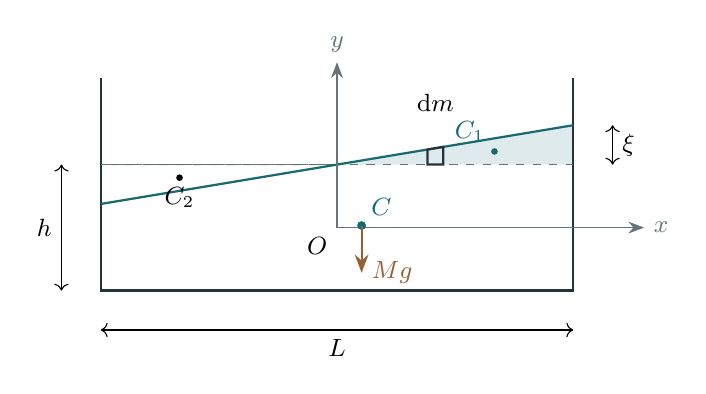
\begin{tikzpicture}[font=\small]
\fill[accent!14](0,.6)--(3,.6)--(3,1.1)--cycle;\draw[guide](-3,.6)--(-3,.1)--(0,.6)--cycle;
\draw[object](-3,1.7)--(-3,-1)--(3,-1)--(3,1.7);
\draw[guide](-3,.6)--(3,.6);\draw[traj](-3,.1)--(3,1.1);
\draw[<->](3.5,.6)--(3.5,1.1)node[midway,right]{$\xi$};
\draw[<->](-3.5,-1)--(-3.5,.6)node[midway,left]{$h$};
\draw[<->](-3,-1.5)--(3,-1.5)node[midway,below]{$L$};
\draw[axis](0,-.2)--(0,1.9)node[above]{$y$};
\draw[axis](0,-.2)--(3.9,-.2)node[right]{$x$};\node[below left]at(0,-.2){$O$};

\fill[accent](2,.766666667)circle(1.2pt)node[above left]{$C_1$};
\fill(-2,.433333333)circle(1.2pt)node[below]{$C_2$};
\draw[object](1.15,.6)--(1.35,.6)--(1.35,.825)--(1.15,.791666667)--cycle;\node[above]at(1.25,1.15){$\dd m$};
\fill[accent](.3125,-.173958333)circle(1.6pt)node[above right]{$C$};
\draw[force](.3125,-.173958333)--(.3125,-.773958333)node[right]{$Mg$};
\end{tikzpicture}\figcaption{解图 7.10A}\end{minipage}\end{center}
取容器宽度为 $b$，液体质量 $M=\rho bLh$。解图7.10A中原点在矩形液体中央，水平为 $x$、竖直为 $y$；右端比静水面升高 $\xi$，左端降低 $\xi$。倾斜面为
\[y_s(x)=h/2+2\xi x/L.\]
将液体看成原矩形加右侧三角块、减左侧三角块。右块微元质量与微元自身中点高度为
\[\dd m=\rho b\frac{2\xi x}{L}\dd x,\qquad y'=h/2+\xi x/L.\]
积分上下限为 $0,L/2$，因此
\[m_1=\rho bL\xi/4,\quad
x_1=\frac{\int_0^{L/2}x^2\dd x}{\int_0^{L/2}x\dd x}=L/3,\quad
y_1=h/2+\xi/3.\]
左侧被减去的三角块有 $m_2=m_1,x_2=-L/3,y_2=h/2-\xi/3$。矩形块质心在原点，故总质心为
\[x_C=\frac{m_1x_1-m_2x_2}{M}=\frac{L\xi}{6h},\qquad
y_C=\frac{m_1y_1-m_2y_2}{M}=\frac{\xi^2}{6h}.\]
其速度分别是 $\dot x_C=L\dot\xi/(6h)$、$\dot y_C=\xi\dot\xi/(3h)$。$\xi\ll h$ 且湖泊狭长时横向质心运动占主导；重力势能增量为 $U=Mg\xi^2/(6h)$。
先采用整体质心运动的近似模型，将内部相对运动动能略去：
\[K_C\simeq\frac M2\dot x_C^2=\frac{ML^2}{72h^2}\dot\xi^2,\qquad
E_C=\frac{ML^2}{72h^2}\dot\xi^2+\frac{Mg}{6h}\xi^2.\]
令此近似能量守恒并求导，得
\[\ddot\xi+\frac{12gh}{L^2}\xi=0,\qquad
\boxed{T_C=\frac{\pi L}{\sqrt{3gh}}.}\]
它预测 $T\propto Lh^{-1/2}$。液面倾角、整体质心的周期相同，但 $K_C$ 不等于液体真实总动能，周期系数的精度由下表中的数据比较确定。
\begin{center}\begin{minipage}{\linewidth}\centering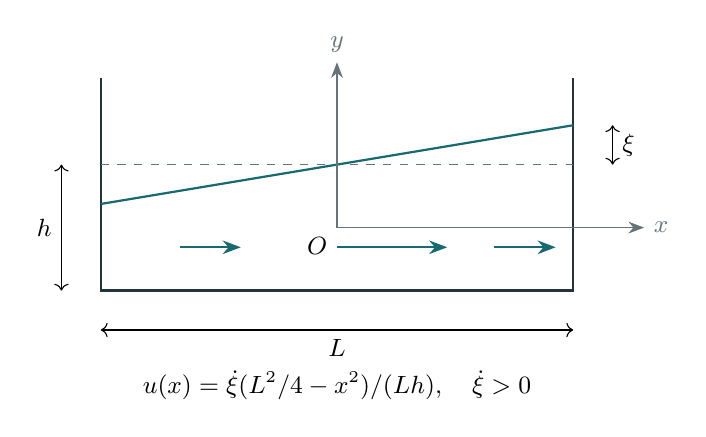
\begin{tikzpicture}[font=\small]
\draw[object](-3,1.7)--(-3,-1)--(3,-1)--(3,1.7);
\draw[guide](-3,.6)--(3,.6);\draw[traj](-3,.1)--(3,1.1);
\draw[<->](3.5,.6)--(3.5,1.1)node[midway,right]{$\xi$};
\draw[<->](-3.5,-1)--(-3.5,.6)node[midway,left]{$h$};
\draw[<->](-3,-1.5)--(3,-1.5)node[midway,below]{$L$};
\draw[axis](0,-.2)--(0,1.9)node[above]{$y$};
\draw[axis](0,-.2)--(3.9,-.2)node[right]{$x$};\node[below left]at(0,-.2){$O$};

\draw[motion](-2,-.45)--(-1.222222222,-.45);
\draw[motion](0,-.45)--(1.4,-.45);
\draw[motion](2,-.45)--(2.777777778,-.45);
\node at(0,-2.2){$u(x)=\dot\xi(L^2/4-x^2)/(Lh),\quad\dot\xi>0$};
\end{tikzpicture}\figcaption{解图 7.10B}\end{minipage}\end{center}
取 $g=9.8\,\mathrm{m/s^2}$，在解图7.10B的同一几何模型下，周期与实测数据比较如下，没有用提前舍入的周期算比值。
\begin{center}\begin{tabular}{r|rrr}\multicolumn{4}{c}{$L=0.479\,\mathrm m$}\\$h/\mathrm{mm}$&$T_{\text{测}}/\mathrm s$&$T_{\rm CM}/\mathrm s$&$T_{\text{测}}/T_{\rm CM}$\\\hline
30&1.78&1.6023&1.1109\\
50&1.40&1.2412&1.1280\\
69&1.18&1.0565&1.1168\\
88&1.08&0.9356&1.1544\\
107&1.00&0.8484&1.1786\\
124&0.91&0.7881&1.1546\\
142&0.82&0.7365&1.1134\\
\end{tabular}\end{center}
\begin{center}\begin{tabular}{r|rrr}\multicolumn{4}{c}{$L=0.143\,\mathrm m$}\\$h/\mathrm{mm}$&$T_{\text{测}}/\mathrm s$&$T_{\rm CM}/\mathrm s$&$T_{\text{测}}/T_{\rm CM}$\\\hline
31&0.52&0.4706&1.1050\\
38&0.48&0.4250&1.1293\\
58&0.43&0.3440&1.2499\\
67&0.35&0.3201&1.0934\\
124&0.28&0.2353&1.1900\\
\end{tabular}\end{center}
两组数据总体随 $h^{-1/2}$ 下降，实测周期大于 $T_C$，全体比值的算术平均约$1.144$；个别点偏离更多。以 $1.15T_C$ 作这组数据的经验修正可以估算量级，却不是新的普适常数。$L=123\,\mathrm{km},h=50\,\mathrm m$ 时，
\[T_C\simeq2.80\,\mathrm h,\qquad 1.15T_C\simeq3.22\,\mathrm h.\]
进一步用速度场计算质心近似之外的内部动能。以底面为 $z=0$，浅水连续性要求
\[\partial_xu=-\frac{\dot\eta}{h}=-\frac{2x\dot\xi}{Lh},\qquad
u(\pm L/2)=0,\]
于是 $u(x)=\dot\xi(L^2/4-x^2)/(Lh)$。速度随截面位置变化，取每一截面的局部速度平方乘对应的水质量元，再求和得到水平动能，
\[K_x=\frac12\rho bh\int_{-L/2}^{L/2}u^2\dd x
=\frac{ML^2}{60h^2}\dot\xi^2>K_C.\]
用该平面液面试探流场得到 $T_{\text{试探}}=2\pi L/\sqrt{10gh}$；它比 $T_C$ 大，说明漏计内部动能会低估周期。更完整的浅水方程为
\[\eta_t+hu_x=0,\quad u_t+g\eta_x=0
\quad\Longrightarrow\quad\eta_{tt}=gh\eta_{xx}.\]
闭合两端的基模 $\eta\propto\cos(\pi x/L)$（此处 $0\le x\le L$）给
\[T_{\text{浅水}}=\frac{2L}{\sqrt{gh}},\qquad
T_{\text{浅水}}/T_C=2\sqrt3/\pi\simeq1.103.\]
湖震是水体的长波驻荡，这个空间基模将整体振荡与浅水波动方程联系起来。平面液面、均匀深度、忽略黏性和复杂岸形都是估算条件；第二组较深容器尤其不满足长浅几何。真实湖泊的周期还随岸形和深度分布变化，这里用平均深度估计时间量级。

\textbf{湖泊记录的相位与时间标度。}
\begin{center}\begin{minipage}{.97\linewidth}\centering
\begin{tikzpicture}[x=.75cm,y=.75cm,font=\small]
\begin{scope}[yshift=4.4cm]
\draw[axis] (0,-.45)--(0,4.1) node[above]{记录读数};
\draw[axis] (0,0)--(10.6,0) node[right]{时间};
\foreach \v in {0,10,20}{\draw (0,{\v/5})--(-.1,{\v/5}) node[left]{$\v$};}
\node at (5.2,3.55){Bastedalen};
\draw[traj] plot coordinates{(0.069,3.6667) (0.1034,3.3158) (0.1379,2.693) (0.1724,2.3333) (0.2069,1.7193) (0.2414,1.1579) (0.2759,0.4561) (0.3103,0.6842) (0.3448,0.9123) (0.3793,1.1404) (0.4138,1.3684) (0.4483,1.5965) (0.4828,1.8246) (0.5172,1.6667) (0.5517,1.5789) (0.5862,1.4912) (0.6207,1.2281) (0.6552,1.0702) (0.6897,0.9474) (0.7241,0.807) (0.7586,0.6667) (0.7931,0.5439) (0.8276,0.4035) (0.8621,0.5088) (0.8966,0.5965) (0.931,0.7018) (0.9655,0.7895) (1.0,0.8947) (1.0345,1.0526) (1.069,1.2105) (1.1034,1.386) (1.1379,1.5789) (1.1724,1.7018) (1.2069,1.8596) (1.2414,1.8246) (1.2759,1.7895) (1.3103,1.5439) (1.3448,1.0702) (1.3793,0.5965) (1.4138,0.5965) (1.4483,0.614) (1.4828,0.614) (1.5172,0.7018) (1.5517,0.8772) (1.5862,1.0526) (1.6207,1.2281) (1.6552,1.4035) (1.6897,1.4737) (1.7241,1.5614) (1.7586,1.6316) (1.7931,1.7018) (1.8276,1.7895) (1.8621,1.8596) (1.8966,1.8947) (1.931,1.8772) (1.9655,1.8596) (2.0,1.8421) (2.0345,1.6667) (2.069,1.3684) (2.1034,1.0702) (2.1379,0.7719) (2.1724,0.7018) (2.2069,0.6491) (2.2414,0.5789) (2.2759,0.5789) (2.3103,0.6316) (2.3448,0.7018) (2.3793,0.7544) (2.4138,0.8246) (2.4483,0.8772) (2.4828,0.9474) (2.5172,1.0) (2.5517,1.1053) (2.5862,1.193) (2.6207,1.2982) (2.6552,1.4035) (2.6897,1.5088) (2.7241,1.5965) (2.7586,1.7018) (2.7931,1.7368) (2.8276,1.7719) (2.8621,1.807) (2.8966,1.5965) (2.931,0.9825) (2.9655,0.8596) (3.0,0.7544) (3.0345,0.6842) (3.069,0.5965) (3.1034,0.6667) (3.1379,0.7368) (3.1724,0.7895) (3.2069,0.8596) (3.2414,0.9298) (3.2759,1.0) (3.3103,1.0877) (3.3448,1.1754) (3.3793,1.2632) (3.4138,1.3333) (3.4483,1.4211) (3.4828,1.5088) (3.5172,1.614) (3.5517,1.6667) (3.5862,1.7544) (3.6207,1.8246) (3.6552,1.4737) (3.6897,1.1053) (3.7241,0.7719) (3.7586,0.614) (3.7931,0.4211) (3.8276,0.0877) (3.8621,-0.193) (3.8966,-0.0877) (3.931,-0.0877) (3.9655,0.1579) (4.0,0.2632) (4.0345,0.4386) (4.069,0.6316) (4.1034,0.8421) (4.1379,1.0351) (4.1724,1.0526) (4.2069,0.8596) (4.2414,0.6667) (4.2759,0.4737) (4.3103,0.3158) (4.3448,0.1579) (4.3793,0.0877) (4.4138,-0.1579) (4.4483,-0.0877) (4.4828,0.0877) (4.5172,0.2105) (4.5517,0.3333) (4.5862,0.4211) (4.6207,0.4912) (4.6552,0.5614) (4.6897,0.6316) (4.7241,0.7368) (4.7586,0.7719) (4.7931,0.8421) (4.8276,0.8772) (4.8621,0.8947) (4.8966,0.9123) (4.931,0.9298) (4.9655,0.9474) (5.0,0.9649) (5.0345,0.9825) (5.069,1.0351) (5.1034,0.9474) (5.1379,0.5965) (5.1724,0.4912) (5.2069,0.386) (5.2414,0.2807) (5.2759,0.1754) (5.3103,0.0877) (5.3448,0.1228) (5.3793,0.193) (5.4138,0.2456) (5.4483,0.3158) (5.4828,0.3684) (5.5172,0.4561) (5.5517,0.5789) (5.5862,0.7018) (5.6207,0.8246) (5.6552,0.9474) (5.6897,1.0) (5.7241,0.9825) (5.7586,0.9649) (5.7931,0.9474) (5.8276,0.7895) (5.8621,0.6316) (5.8966,0.4737) (5.931,0.3158) (5.9655,0.2105) (6.0,0.1579) (6.0345,0.1053) (6.069,0.0877) (6.1034,0.1228) (6.1379,0.1754) (6.1724,0.2456) (6.2069,0.3158) (6.2414,0.3684) (6.2759,0.4737) (6.3103,0.5965) (6.3448,0.7193) (6.3793,0.8596) (6.4138,0.9825) (6.4483,0.8772) (6.4828,0.7719) (6.5172,0.6667) (6.5517,0.5614) (6.5862,0.4737) (6.6207,0.3684) (6.6552,0.2807) (6.6897,0.1754) (6.7241,0.0877) (6.7586,0.1404) (6.7931,0.1053) (6.8276,0.2695) (6.8621,0.3301) (6.8966,0.2982) (6.931,0.3333) (6.9655,0.4035) (7.0,0.4561) (7.0345,0.5614) (7.069,0.614) (7.1034,0.6316) (7.1379,0.6842) (7.1724,0.7368) (7.2069,0.7544) (7.2414,0.7544) (7.2759,0.7544) (7.3103,0.7368) (7.3448,0.7018) (7.3793,0.6491) (7.4138,0.5965) (7.4483,0.5263) (7.4828,0.4386) (7.5172,0.3509) (7.5517,0.2632)};
\draw[traj] plot coordinates{(7.8621,-0.0175) (7.8966,0.0205) (7.931,0.0585) (7.9655,0.1053) (8.0,0.1404) (8.0345,0.1754) (8.069,0.2105) (8.1034,0.2456) (8.1379,0.2632) (8.1724,0.2982) (8.2069,0.3333) (8.2414,0.3684) (8.2759,0.386) (8.3103,0.4211)};
\draw[guide] (1.88,-.25)--(1.88,2.3) (2.88,-.25)--(2.88,2.3);
\draw[<->] (1.88,2.55)--(2.88,2.55) node[midway,above]{$T$};
\node[below] at (1.88,-.2){$P_1$};\node[below] at (2.88,-.2){$P_2$};
\end{scope}
\draw[axis] (0,-.25)--(0,4.15) node[above]{记录读数};
\draw[axis] (0,0)--(10.6,0) node[right]{时间};
\foreach \v in {0,10,20}{\draw (0,{\v/5})--(-.1,{\v/5}) node[left]{$\v$};}
\node at (5.3,3.95){J\"onk\"oping};
\draw[traj] plot coordinates{(0.0517,1.1228) (0.0862,1.4486) (0.1207,1.7744) (0.1552,2.1003) (0.1897,2.3225) (0.2241,2.4413) (0.2586,2.5601) (0.2931,2.6788) (0.3276,2.7976) (0.3621,2.9163) (0.3966,3.1754) (0.431,3.2456) (0.4655,3.3684) (0.5,3.5263) (0.5345,3.1404) (0.569,2.7368) (0.6034,2.5088) (0.6379,2.4211) (0.6724,2.3333) (0.7069,2.2456) (0.7414,2.1579) (0.7759,2.0702) (0.8103,2.2632) (0.8448,2.4737) (0.8793,2.6667) (0.9138,2.8596) (0.9483,2.9825) (0.9828,3.0175) (1.0172,3.0877) (1.0517,3.0702) (1.0862,3.0526) (1.1207,2.9825) (1.1552,2.8947) (1.1897,2.807) (1.2241,2.5789) (1.2586,2.3509) (1.2931,2.1228) (1.3276,1.9825) (1.3621,1.9649) (1.3966,1.9298) (1.431,1.9123) (1.4655,2.0351) (1.5,2.1579) (1.5345,2.2807) (1.569,2.4035) (1.6034,2.4912) (1.6379,2.5965) (1.6724,2.7193) (1.7069,2.7895) (1.7414,2.807) (1.7759,2.8246) (1.8103,2.7719) (1.8448,2.7193) (1.8793,2.4912) (1.9138,2.0526) (1.9483,2.193) (1.9828,2.3509) (2.0172,2.4912) (2.0517,2.5789) (2.0862,2.614) (2.1207,2.6491) (2.1552,2.6667) (2.1897,2.7018) (2.2241,2.7368) (2.2586,2.7544) (2.2931,2.7719) (2.3276,2.7719) (2.3621,2.5614) (2.3966,2.3333) (2.431,2.1228) (2.4655,2.0351) (2.5,1.9474) (2.5345,1.8596) (2.569,1.9474) (2.6034,2.0526) (2.6379,2.1404) (2.6724,2.2281) (2.7069,2.3509) (2.7414,2.4737) (2.7759,2.5965) (2.8103,2.7193) (2.8448,2.7719) (2.8793,2.7544) (2.9138,2.7193) (2.9483,2.6842) (2.9828,2.6316) (3.0172,2.5789) (3.0517,2.5263) (3.0862,2.4737) (3.1207,2.2281) (3.1552,2.0175) (3.1897,2.0351) (3.2241,2.0702) (3.2586,2.0877) (3.2931,2.1228) (3.3276,2.2105) (3.3621,2.2982) (3.3966,2.386) (3.431,2.4737) (3.4655,2.5614) (3.5,2.6316) (3.5345,2.7018) (3.569,2.7544) (3.6034,2.8246) (3.6379,2.8947) (3.6724,2.7368) (3.7069,2.5614) (3.7414,2.4737) (3.7759,2.3684) (3.8103,2.2807) (3.8448,2.1754) (3.8793,2.0877) (3.9138,2.1754) (3.9483,2.2632) (3.9828,2.3509) (4.0172,2.4386) (4.0517,2.5614) (4.0862,2.6842) (4.1207,2.807) (4.1552,2.9298) (4.1897,2.9474) (4.2241,2.9649) (4.2586,3.0) (4.2931,3.0175) (4.3276,3.0351) (4.3621,2.9825) (4.3966,2.7895) (4.431,2.6667) (4.4655,2.5614) (4.5,2.4561) (4.5345,2.3684) (4.569,2.2632) (4.6034,2.2456) (4.6379,2.2807) (4.6724,2.3509) (4.7069,2.4386) (4.7414,2.5088) (4.7759,2.5439) (4.8103,2.5789) (4.8448,2.5789) (4.8793,2.614) (4.9138,2.6667) (4.9483,2.7368) (4.9828,2.7719) (5.0172,2.8596) (5.0517,2.9298) (5.0862,3.0) (5.1207,3.0702) (5.1552,3.1404) (5.1897,3.1228) (5.2241,3.0351) (5.2586,2.9298) (5.2931,2.8421) (5.3276,2.5088) (5.3621,2.1579) (5.3966,2.2105) (5.431,2.2807) (5.4655,2.386) (5.5,2.4561) (5.5345,2.5439) (5.569,2.6316) (5.6034,2.7018) (5.6379,2.7895) (5.6724,2.8772) (5.7069,2.8596) (5.7414,2.8596) (5.7759,2.8421) (5.8103,2.8246) (5.8448,2.7719) (5.8793,2.6667) (5.9138,2.5614) (5.9483,2.4561) (5.9828,2.386) (6.0172,2.3333) (6.0517,2.2982) (6.0862,2.2456) (6.1207,2.2105) (6.1552,2.2456) (6.1897,2.2807) (6.2241,2.3333) (6.2586,2.3684) (6.2931,2.4211) (6.3276,2.4912) (6.3621,2.5614) (6.3966,2.6491) (6.431,2.7193) (6.4655,2.7895) (6.5,2.8596) (6.5345,2.8596) (6.569,2.8772) (6.6034,2.8772) (6.6379,2.7368) (6.6724,2.5789) (6.7069,2.4386) (6.7414,2.3509) (6.7759,2.3333) (6.8103,2.2982) (6.8448,2.2632) (6.8793,2.2456) (6.9138,2.2281) (6.9483,2.2456) (6.9828,2.2632) (7.0172,2.2632) (7.0517,2.2807) (7.0862,2.3333) (7.1207,2.386) (7.1552,2.4211) (7.1897,2.4737) (7.2241,2.5263) (7.2586,2.5789) (7.2931,2.6316) (7.3276,2.7018) (7.3621,2.7719) (7.3966,2.8421) (7.431,2.9123) (7.4655,2.9825) (7.5,2.9825) (7.5345,2.8947) (7.569,2.8246) (7.6034,2.7368) (7.6379,2.6316) (7.6724,2.5263) (7.7069,2.4386) (7.7414,2.3333) (7.7759,2.2281) (7.8103,2.1579) (7.8448,2.1053) (7.8793,2.0702) (7.9138,2.0) (7.9483,1.9474) (7.9828,1.8772) (8.0172,1.8246) (8.0517,1.7895) (8.0862,1.7544) (8.1207,1.7193) (8.1552,1.6842) (8.1897,1.6491) (8.2241,1.614) (8.2586,1.5789) (8.2931,1.5439)};
\node[align=left] at (7.9,1.0){各记录保留自己的读数零点\\横轴没有数值时间刻度};
\end{tikzpicture}\figcaption{解图 7.10C　上图相邻较清楚的峰$P_1,P_2$之间约为一次振荡；两记录的纵轴零点分别保留。}\end{minipage}\end{center}
解图7.10C中，上端记录起初下降、下端记录起初上升，两处都有数次往复，但振幅、基线和局部波形不同。模型的长波基模预期两端相反，$\eta(0,t)=-\eta(L,t)$；比较两端相位时，将两条记录按同一时间标记对齐，并各自减去平均液面。图中两记录保留各自的读数零点，且未标共同绝对起点；当前记录给出多次往复的形状，可能含多个模态，进一步的峰谷配对和水量分析需要同步、统一基准的位移。

记录横轴保留了相邻峰的相对间距，绝对秒数另需时间标记。模型给出的约3小时是单次主要振荡的时间标度：质心近似$2.80\,\mathrm h$，容器数据经验修正约$3.22\,\mathrm h$，浅水基模则为$2L/\sqrt{gh}\simeq3.09\,\mathrm h$。因此$P_1P_2$所示的一次较完整往复应以数小时标定；三种估算给出不同模型的时间标度，图上一次峰间距对应单次振荡的数小时量级。
\subsubsection*{三角水块与总质心的积分全步}
解图7.10A用右侧实三角块表示增加的水，左侧虚三角块表示扣去的水。
宽度$b$保持在每个质量微元中，最后才约去。
对$\xi>0$，右块质量为
\[
m_1=\frac{2\rho b\xi}{L}\int_0^{L/2}x\dd x
=\frac{2\rho b\xi}{L}\left[\frac{x^2}{2}\right]_0^{L/2}
=\frac{\rho bL\xi}{4}.
\]
右块的两个一次矩为
\[
\begin{aligned}
m_1x_1&=\frac{2\rho b\xi}{L}\left[\frac{x^3}{3}\right]_0^{L/2}
=\frac{\rho b\xi L^2}{12},\\
m_1y_1&=\frac h2m_1+
\frac{2\rho b\xi^2}{L^2}\left[\frac{x^3}{3}\right]_0^{L/2}
=m_1\left(\frac h2+\frac\xi3\right).
\end{aligned}
\]
左块是被减去的体积，故其质量用正数$m_2=m_1$表示，
但在总一次矩中带负号。
它的横坐标为$-L/3$，于是减去左块的负横矩会使总横矩增加；
右增块的正横矩与减去左块的负横矩同向相加，使$x_C$向右。
逐项合并得
\[
\begin{aligned}
M&=\rho bLh+m_1-m_2=\rho bLh,\\
Mx_C&=m_1(L/3)-m_1(-L/3)=\rho b\xi L^2/6,\\
My_C&=m_1(h/2+\xi/3)-m_1(h/2-\xi/3)
=\rho bL\xi^2/6.
\end{aligned}
\]
当$\xi$改变符号时两端角色互换，$x_C$为奇函数、$y_C$为偶函数，
所以这两个质心表达式连续适用于整个小振动。
静水面时$y_C=0$，倾斜后$y_C>0$，重力势能有极小，回复方向正确。

\subsubsection*{质心近似的阶数与能量求导}
由质心坐标分别得到
\[
\left|\frac{y_C}{x_C}\right|=\frac{|\xi|}{L},\qquad
\left|\frac{\dot y_C}{\dot x_C}\right|=\frac{2|\xi|}{L},\qquad
\frac{K_{Cy}}{K_{Cx}}=\frac{4\xi^2}{L^2}.
\]
因此忽略质心竖直动能要求$|\xi|\ll L$；
题给$|\xi|\ll h$配合$h\ll L$足以保证它。
全水体动能还含水元相对质心的运动，其二阶贡献在小振幅下与质心动能同阶。

在明确采用质心动能模型后，对其能量完整求导，
\[
0=\dot E_C=\frac{ML^2}{36h^2}\dot\xi\ddot\xi
+\frac{Mg}{3h}\xi\dot\xi
=\frac{ML^2}{36h^2}\dot\xi
\left(\ddot\xi+\frac{12gh}{L^2}\xi\right).
\]
先在$\dot\xi\ne0$段得到方程，再连续延伸到两端。
若初态右端升高$\xi_0$、全水静止，则
\[
\xi(t)=\xi_0\cos(\sqrt{12gh}\,t/L),\quad
x_C(t)=\frac{L\xi_0}{6h}\cos(\sqrt{12gh}\,t/L).
\]
液面端点与横向质心同周期；
$y_C\propto\cos^2(\sqrt{12gh}\,t/L)$则含二倍频，
竖直质心在一个液面周期内有两次极小，液面端点的一次完整往复仍取基频周期。

\subsubsection*{连续性、内部动能与平面液面的限制}
解图7.10B把水深方向平均流速记为$u(x,t)$。
从$\eta=2\xi x/L$和两端不透水条件积分，
\[
u_x=-\frac{2x\dot\xi}{Lh},\quad
u=-\frac{x^2\dot\xi}{Lh}+C(t),\quad
C=\frac{L\dot\xi}{4h}.
\]
两端同为零，中部流速最大，与图中箭头一致。
横向速度的空间平均是
\[
\bar u=\frac1L\int_{-L/2}^{L/2}u\dd x
=\frac{L\dot\xi}{6h}=\dot x_C,
\]
而平方积分须展开四次多项式，
\[
\int_{-L/2}^{L/2}(L^2/4-x^2)^2\dd x
=\frac{L^5}{16}-\frac{L^5}{24}+\frac{L^5}{80}
=\frac{L^5}{30}.
\]
于是$K_x/K_{Cx}=6/5$，
\[
K_x-K_{Cx}=\frac{ML^2}{360h^2}\dot\xi^2>0.
\]
这部分就是相对质心的内部水平动能，和振幅同为二阶，
在振幅趋零时仍占固定比例。
相同势能下，试探周期比为$\sqrt{6/5}$，约增$9.54\%$，
给出漏计内部动能时周期偏小的定量修正，实验的其余差异还涉及水深、激发模态和容器条件。

以底面$z=0$，由不可压缩和底面不透水，
\[
w_z=-u_x,\quad w(x,0)=0
\quad\Longrightarrow\quad w=\frac{2xz\dot\xi}{Lh}.
\]
它在$z=h$满足线性自由面运动条件$w=\eta_t$，
对应竖直动能$K_z=M\dot\xi^2/18$，
与$K_x$之比为$10h^2/(3L^2)$。
小幅条件由$\xi/h$控制，竖直动能相对水平动能的量级则由$h/L$控制。
该流场只满足所取液面形状的连续性；
其$u_t$随$x$呈抛物线，而平面液面的$-g\eta_x$与$x$无关，
两者在$x$上的形状不同，因而这一平面液面流场满足连续性，却是水平动量方程的试探近似。自由面本征解的空间形状由完整方程和壁面条件确定。

\subsubsection*{逐行周期比与有限水深基模}
表中毫米先换算成米再计算。两组$T/T_C$的平均值分别为
$1.13668$和$1.15354$；全部12点的算术平均为$1.14370$。
用$1.15$作便于估算的经验因子可以描述总体偏差，
这个取值与数据平均略有区别，适用范围限于这里的经验估计。
第一组比值约在$1.111$至$1.179$间，
第二组约在$1.093$至$1.250$间；数据离散程度不应被一个修正系数掩盖。

两组的水深与长度比分别为：第一组$h/L$从$0.063$到$0.296$，
第二组从$0.217$到$0.867$，后一组较深端的$h/L$已为一阶量，应使用保留有限水深的公式。
在不可压缩、无旋、小振幅、矩形自由液面的模型中，
取$0\le X\le L$、底面$z=0$，基模波数$\kappa=\pi/L$。
底面条件使速度势的竖直形状为$\cosh(\kappa z)$；
令
\[
\begin{aligned}
\eta&=a\cos(\kappa X)\cos\omega t,\\
\Phi&=-\frac{ga}{\omega}\cos(\kappa X)
\frac{\cosh(\kappa z)}{\cosh(\kappa h)}\sin\omega t.
\end{aligned}
\]
它在两端满足$\Phi_X=0$，在底面满足$\Phi_z=0$，
自由面动态条件$\Phi_t+g\eta=0$也成立。
再用$\eta_t=\Phi_z$得到
\[
\omega_1^2=g\kappa\tanh(\kappa h),\qquad
T_1=\frac{2\pi}{\sqrt{g\kappa\tanh(\kappa h)}}.
\]
当$\kappa h\ll1$，$\tanh(\kappa h)\simeq\kappa h$，
恢复$2L/\sqrt{gh}$。在深水极限，
$T_1\to2\sqrt{\pi L/g}$，周期不会随深度无限下降。
例如$L=0.143\,\mathrm m$时此下限约$0.4282\,\mathrm s$，
而给定深端的$0.35\,\mathrm s$、$0.28\,\mathrm s$均低于该下限。
这两个深端数据已超出同一自由面基模的周期范围。它们的解释需要实际激发模态、有效长度和容器条件；当前给定数据支持的是模型量级与比例的比较。

最后将$123\,\mathrm{km}=123000\,\mathrm m$代入，
质心模型给$10078.5\,\mathrm s=2.7996\,\mathrm h$，
乘$1.15$得$3.2195\,\mathrm h$，浅水基模给$3.0870\,\mathrm h$。
解图7.10C的相邻峰距应以单次约三小时标定，
整段记录则覆盖多次这样的往复。
真实湖泊的深度和岸线不均匀，以上数字用于时间量级估计。



\Needspace{18\baselineskip}

\pdfbookmark[2]{第 11 题 滑块摆系统的轨迹与小角振动}{q11}

\section*{第 11 题\quad 滑块摆系统的轨迹与小角振动}

\tagline{M-07-11}

如图,质量为\(m_{1}\)的滑块可在光滑水平直导轨上滑动.滑块经长为\(l\)质量可略的细杆

与质量为 \(m_{2}\) 的重锤相连,细杆与重锤可绕滑块无摩擦地自由转动.设
\(t=0\) 时,细杆与导轨构成铅垂面,细杆与铅锤线夹角
\(\theta_{0}\),从静止释放开始摆动.试求:1.重锤 \(m_{2}\)
的运动轨迹.2.系统作小角摆动时,滑块位置随时间的变化.

\begin{center}\begin{minipage}{\linewidth}\centering\begin{tikzpicture}[font=\small]
\draw[object](-2.6,0)--(2.6,0);\draw[object,fill=white](-.697618262,-.15)rectangle(-.147618262,.15);
\node[above]at(-.422618262,.25){$m_1$};
\draw[object](-.422618262,0)--(.845236523,-2.718923361);
\fill[accent](.845236523,-2.718923361)circle(2.5pt)node[right]{$m_2$};
\draw[guide](-.422618262,0)--(-.422618262,-1.25);
\draw[motion](-.422618262,-.65)arc(-90:-65:.65);\node at(-.13,-.95){$\theta$};
\node[right]at(.35,-1.55){$l$};
\draw[axis](-2.3,.8)--(-1.2,.8)node[right]{$x$};
\end{tikzpicture}\figcaption{图 7.11}\end{minipage}\end{center}

\Needspace{18\baselineskip}\subsection*{解答}

\begin{center}\begin{minipage}{\linewidth}\centering\begin{tikzpicture}[font=\small]
\draw[object](-2.6,0)--(2.6,0);\draw[object,fill=white](-.697618262,-.15)rectangle(-.147618262,.15);
\node[above]at(-.422618262,.25){$m_1$};
\draw[object](-.422618262,0)--(.845236523,-2.718923361);
\fill[accent](.845236523,-2.718923361)circle(2.5pt)node[right]{$m_2$};
\draw[guide](-.422618262,0)--(-.422618262,-1.25);
\draw[motion](-.422618262,-.65)arc(-90:-65:.65);\node at(-.13,-.95){$\theta$};
\node[right]at(.35,-1.55){$l$};

\draw[axis](0,0)--(2.6,0)node[right]{$x$};\draw[axis](0,0)--(0,-3.5)node[below]{$y$};
\node[above right]at(0,0){$O$};
\draw[traj,domain=-25:25,samples=65]plot({2*sin(\x)},{-3*cos(\x)});
\fill[accent](0,-.906307787)circle(1.5pt)node[right]{$C$};
\node[above]at(.4,.75){示意$m_1=2m_2$，质心只沿竖线移动};
\draw[force](.845236523,-2.718923361)--(.845236523,-3.35)node[right]{$m_2g$};
\end{tikzpicture}\figcaption{解图 7.11A}\end{minipage}\end{center}
设 $l_1$ 为滑块到系统质心的距离，$l_2$ 为重锤到质心的距离。由 $m_1l_1=m_2l_2$、$l_1+l_2=l$，
\[l_1=\frac{m_2l}{m_1+m_2},\qquad l_2=\frac{m_1l}{m_1+m_2}.\]
水平外力为零且初始总动量为零，系统质心水平坐标固定。以该垂线与导轨交点为原点，$y$ 向下，几何约束给
\[x_1=-l_1\sin\theta,\qquad x_2=l_2\sin\theta,\qquad y_2=l\cos\theta.\]
消去 $\theta$ 得重锤轨迹
\[\boxed{\frac{x_2^2}{l_2^2}+\frac{y_2^2}{l^2}=1.}\]
解图7.11A画的是椭圆下半部上由实际摆幅截取的一段；质心的高度仍可变化，只有水平位置固定。
\par\textbf{能量法。} 对几何式求导，
\[\dot x_1=-l_1\cos\theta\dot\theta,\quad
\dot x_2=l_2\cos\theta\dot\theta,\quad
\dot y_2=-l\sin\theta\dot\theta.\]
令 $A=m_1l_1^2+m_2l_2^2=m_1m_2l^2/(m_1+m_2)$，则完整机械能为
\[E=\frac12[A\cos^2\theta+m_2l^2\sin^2\theta]\dot\theta^2
-m_2gl\cos\theta.\]
用 $D(\theta)=A\cos^2\theta+m_2l^2\sin^2\theta$，对时间求导得到
\[D\ddot\theta+\frac12D'\dot\theta^2+m_2gl\sin\theta=0.\]
微小振动时 $D=A+O(\theta^2)$，$D'\dot\theta^2$ 为高阶，故
\[\ddot\theta+\frac{(m_1+m_2)g}{m_1l}\theta=0,\qquad
\Omega=\sqrt{\frac{(m_1+m_2)g}{m_1l}}.\]
由从 $\theta_0$ 静止释放，$\theta=\theta_0\cos\Omega t$，滑块的位置为
\[\boxed{x_1(t)\simeq-\frac{m_2l}{m_1+m_2}\theta_0\cos\Omega t.}\]
若以滑块初始位置为坐标原点，则右端再加 $l_1\theta_0$；原点选择同时确定了这一常量位移。
\par\textbf{滑块系另解。} 滑块的加速度为 $a_1$，重锤切向方程含惯性力：
\[m_2l\ddot\theta=-m_2g\sin\theta-m_2a_1\cos\theta.\]
水平动量和相对运动给一阶 $a_1=-m_2l\ddot\theta/(m_1+m_2)$，代回并取 $\cos\theta\simeq1,\sin\theta\simeq\theta$，得到同一 $\Omega$。
\par\Needspace{9\baselineskip}\textbf{质心附近另解。} 质心竖直位移是二阶，小振动中可暂视其固定。杆张力一阶近似为 $T\simeq m_2g$，滑块方程
\[m_1\ddot x_1=T\sin\theta\simeq m_2g\theta
=-\frac{m_2g}{l_1}x_1\]
仍给 $\ddot x_1+[(m_1+m_2)g/(m_1l)]x_1=0$。第三法取一阶运动，有限角则按前面的完整能量及质心坐标求解。
\subsubsection*{质心垂线、椭圆弧与初始原点}
解图7.11A以水平质心垂线为$y$轴，向下为正。
图示取$m_1=2m_2$，故$l_1=l/3,l_2=2l/3$；
一般质量比时仍由前述质心关系确定两段长度。
初始总水平动量为零，任何时刻均有
\[
m_1\dot x_1+m_2\dot x_2=0,\quad
m_1x_1+m_2x_2=0,\quad x_2-x_1=l\sin\theta.
\]
把$x_2=x_1+l\sin\theta$代入第二式，
\[
(m_1+m_2)x_1=-m_2l\sin\theta,
\quad x_2=\frac{m_1l}{m_1+m_2}\sin\theta.
\]
再以杆的竖直投影给$y_2=l\cos\theta$，
两坐标平方相加才消去摆角得到椭圆。
从静止释放且$|\theta_0|<\pi$时，能量只允许两端$\pm\theta_0$之间的摆弧；
运动范围由释放能量给定，时间规律由下面的能量方程求出。
固定的是质心横坐标，质心纵坐标为$y_C=l_1\cos\theta$，
相对最低构型的变化为$l_1(\cos\theta-1)$，小角时从二阶开始。

若采用滑块初位置为原点，则精确相对位移为
\[
\Delta x_1=-l_1(\sin\theta-\sin\theta_0).
\]
小角代入后为$l_1\theta_0(1-\cos\Omega t)$，
在$t=0$确为零；横向质心原点下的$x_1(0)$却为负。
横向质心原点下，正振幅对应初相位$\pi$；换到初位置原点，再加入上述常量位移。

\subsubsection*{能量法中惯量与导数的全展开}
先将各方向动能逐项相加，水平部分的系数为
\[
m_1l_1^2+m_2l_2^2
=\frac{m_1m_2^2l^2+m_2m_1^2l^2}{(m_1+m_2)^2}
=\frac{m_1m_2l^2}{m_1+m_2}=A.
\]
竖直部分只由重锤贡献，系数为$m_2l^2\sin^2\theta$。
由此
\[
D'=2(m_2l^2-A)\sin\theta\cos\theta,
\quad m_2l^2-A=\frac{m_2^2l^2}{m_1+m_2}.
\]
对能量完整求导，
\[
\dot E=\dot\theta\left[D\ddot\theta+
(m_2l^2-A)\sin\theta\cos\theta\dot\theta^2
+m_2gl\sin\theta\right]=0.
\]
在非转折点约去$\dot\theta$，转折点由连续性恢复。
小角下保留一阶项，
$A\ddot\theta+m_2gl\theta=0$；
代$A$后分别约去$m_2l$，得到
$\Omega^2=(m_1+m_2)g/(m_1l)$。
由$\theta(0)=\theta_0,\dot\theta(0)=0$，
角度的初相位为零，而$x_1=-l_1\theta$的初相位相差$\pi$。

\subsubsection*{滑块参考系的加速度消元全步}
在随滑块平移而不转动的系中，重锤除重力、杆力外，
还受$-m_2a_1$的水平惯性力。
切向正向取增大$\theta$，杆力没有切向分量，故
\[
m_2l\ddot\theta=-m_2g\sin\theta-m_2a_1\cos\theta.
\]
同时，地面系水平加速度关系为
\[
m_1a_1+m_2a_2=0,\qquad
a_2-a_1=l(\cos\theta\ddot\theta-\sin\theta\dot\theta^2).
\]
第一式给$a_2=-m_1a_1/m_2$，代第二式才得
\[
a_1=-\frac{m_2l}{m_1+m_2}
(\cos\theta\ddot\theta-\sin\theta\dot\theta^2).
\]
有限角时相对水平加速度同时含切向投影和向心投影。
把完整$a_1$代切向式，
\[
\left[l-\frac{m_2l}{m_1+m_2}\cos^2\theta\right]\ddot\theta
+\frac{m_2l}{m_1+m_2}\sin\theta\cos\theta\dot\theta^2
+g\sin\theta=0.
\]
全式乘$m_2l$后，第一项系数恰为$D$，
第二项系数恰为$D'/2$，与能量法逐项一致。
最后才令$\cos\theta\simeq1,\sin\theta\simeq\theta$，
\[
\frac{m_1l}{m_1+m_2}\ddot\theta+g\theta=0,
\]
恢复同一频率。这样保留了移动悬点的惯性作用，
支点加速度通过惯性力进入重锤的切向方程。

\subsubsection*{质心附近方法与小质量滑块的限制}
第三种方法只保留一阶运动。
$y_C-l_1=-l_1\theta^2/2+\cdots$为二阶，
所以质心系的竖直惯性修正暂不进入线性式。
杆力的零阶值为$T=m_2g$，滑块的水平式给
\[
m_1\ddot x_1=T\sin\theta\simeq m_2g\theta,
\quad\theta\simeq-x_1/l_1.
\]
合并得
\[
\ddot x_1+\frac{m_2g}{m_1l_1}x_1=0,
\quad\frac{m_2g}{m_1l_1}=\frac{(m_1+m_2)g}{m_1l}.
\]
用$x_1(0)=-l_1\theta_0,\dot x_1(0)=0$定常数，
正振幅为$l_1\theta_0$，相位为$\pi$。
有限角质心纵坐标仍为$l_1\cos\theta$，重锤轨迹保持前面求出的椭圆弧。

质量比极端时，角度惯性的近似还含一个控制参数。令$q=m_2/m_1$，
\[
D=A(1+q\sin^2\theta).
\]
当 $|\theta_0|\ll1$ 且 $q\theta_0^2\ll1$ 时，角度惯性可取常量 $A$。滑块越轻，$q=m_2/m_1$ 越大，这个近似允许的摆角就越小。有限摆幅下保留 $D(\theta)$，用完整能量式求周期。
由完整能量可保留周期积分，
\[
T=4\int_0^{\theta_0}
\sqrt{\frac{D(\theta)}{2m_2gl(\cos\theta-\cos\theta_0)}}\,\dd\theta.
\]
在上述两个小量条件下作展开，
$T/T_0=1+(1/16+q/4)\theta_0^2+\cdots$，
显示自由悬点的有限幅修正还受质量比控制。


\Needspace{18\baselineskip}

\pdfbookmark[2]{第 12 题 实心球在球形碗底纯滚动的小振动}{q12}

\section*{第 12 题\quad 实心球在球形碗底纯滚动的小振动}

\tagline{M-07-12}

如图,质量为 \(m\),半径为 \(r\) 的均匀实心小球在半径为 \(R\)
的球形碗底作纯滚动.试求微小振动的周期.

\begin{center}\begin{minipage}{\linewidth}\centering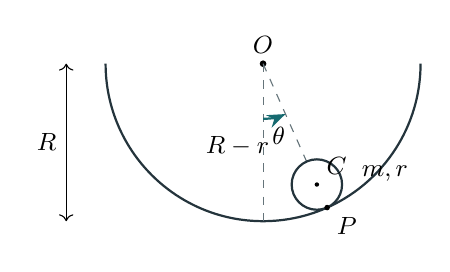
\begin{tikzpicture}[font=\small]
\draw[object](-2,0)arc(180:360:2);\fill(0,0)circle(1.2pt)node[above]{$O$};
\draw[guide](0,0)--(.813473286,-1.827090915);\draw[guide](0,0)--(0,-2);
\draw[object,fill=white](.683317561,-1.534756369)circle(.32);
\fill(.683317561,-1.534756369)circle(.8pt)node[above right]{$C$};
\fill(.813473286,-1.827090915)circle(1pt)node[below right]{$P$};
\draw[motion](0,-.7)arc(-90:-66:.7);\node at(.2,-.92){$\theta$};
\draw[<->](-2.5,0)--(-2.5,-2)node[midway,left]{$R$};
\node[left]at(.2,-1.05){$R-r$};\node[right]at(1.13,-1.4){$m,r$};
\end{tikzpicture}\figcaption{图 7.12}\end{minipage}\end{center}

\Needspace{18\baselineskip}\subsection*{解答}

\begin{center}\begin{minipage}{\linewidth}\centering\begin{tikzpicture}[font=\small]
\draw[object](-2,0)arc(180:360:2);\fill(0,0)circle(1.2pt)node[above]{$O$};
\draw[guide](0,0)--(.813473286,-1.827090915);\draw[guide](0,0)--(0,-2);
\draw[object,fill=white](.683317561,-1.534756369)circle(.32);
\fill(.683317561,-1.534756369)circle(.8pt)node[above right]{$C$};
\fill(.813473286,-1.827090915)circle(1pt)node[below right]{$P$};
\draw[motion](0,-.7)arc(-90:-66:.7);\node at(.2,-.92){$\theta$};
\draw[<->](-2.5,0)--(-2.5,-2)node[midway,left]{$R$};
\node[left]at(.2,-1.05){$R-r$};\node[right]at(1.05,-.45){$m,r$};\draw[guide](.86,-1.27)--(1.15,-.6);

\draw[force](.683317561,-1.534756369)--(.683317561,-3.334756369)node[right]{$mg$};
\draw[force](.813473286,-1.827090915)--(.144642943,-.324873369)node[left]{$N$};
\draw[force](.813473286,-1.827090915)--(1.004567670,-1.742010214)node[above right]{$f$};
\node at(.1,-3.9){示意右端静止释放：$\theta=24^\circ,\quad f>0$沿上坡};
\end{tikzpicture}\figcaption{解图 7.12A}\end{minipage}\end{center}
小球质心绕碗心运动的半径为 $a=R-r$，由两球面的内切几何确定。以偏离碗底的轨道角 $\theta$ 为变量，切向朝增大 $\theta$ 的方向为正，摩擦 $f$ 也按该方向记符号。切向平移、绕心转动与无滑条件给
\[ma\ddot\theta=-mg\sin\theta+f,\qquad
f=-\frac{I}{r^2}a\ddot\theta,\qquad I=\frac25mr^2.\]
消去摩擦：
\[\frac75ma\ddot\theta=-mg\sin\theta,\qquad
\ddot\theta+\frac{5g}{7(R-r)}\sin\theta=0.\]
在线性近似 $\sin\theta\simeq\theta$ 下，
\[\boxed{\Omega=\sqrt{\frac{5g}{7(R-r)}},\qquad
T=2\pi\sqrt{\frac{7(R-r)}{5g}}.}\]
解图7.12A中的轨道角与小球顺时针自旋角$\varphi$是不同变量；$r|\dot\varphi|=a|\dot\theta|$。
能量另解为
\[E=\frac12m a^2\dot\theta^2+\frac12I\left(\frac ar\dot\theta\right)^2
+mga(1-\cos\theta)
=\frac7{10}ma^2\dot\theta^2+mga(1-\cos\theta).\]
小角时势能为 $mga\theta^2/2$，求导给 $(7/5)ma^2\ddot\theta+mga\theta=0$，与动力学一致。
从动力学式还能把摩擦的作用解释清楚。消元后$a\ddot\theta=-(5/7)g\sin\theta$，代回转动约束得
\[f=-\frac25ma\ddot\theta=\frac27mg\sin\theta.\]
在右侧$\theta>0$时，重力使球向碗底加速，摩擦向上坡以增加自旋。摩擦减小质心加速度，同时增大自转角速度：固定碗面上的接触点瞬时不滑动，摩擦的平动功与转动功相互抵消。解图7.12A中的球心轨道运动与球面自旋分别对应这两项动能。

所需摩擦大小为 $|f|=2mg|\sin\theta|/7$；法向压力为 $N=mg\cos\theta+ma\dot\theta^2$。纯滚需 $|f|\le\mu_sN$，对足够小的振幅可以满足。$R>r$ 给出正的球心轨道半径；角幅远小于一弧度，接触斑尺寸远小于轨道半径，采用小角、刚性点接触模型。
\subsubsection*{接触几何与两种转角的符号}
图7.12与解图7.12A标出碗心$O$、球心$C$和接触点$P$。
三点共线，$OP=R,CP=r$，因此$OC=a=R-r$。
质心沿$OC$的圆弧移动，而接触点位于半径$R$的碗面，
两条弧的半径分别为$a$与$R$，滚动条件使用球心速度和球面自旋的接触点速度。
取$\theta$从碗底竖直方向向右增加，
球心速度沿$\hat{\boldsymbol t}$，大小为$a\dot\theta$。
自旋角$\varphi$取顺时针为正，实际矢量自旋角速度为
$\boldsymbol\omega_s=-\dot\varphi\hat{\boldsymbol z}$。
接触点的速度为
\[
\boldsymbol v_P=\boldsymbol v_C+\boldsymbol\omega_s\times\boldsymbol r_{CP}
=(a\dot\theta-r\dot\varphi)\hat{\boldsymbol t}=0.
\]
所以$r\dot\varphi=a\dot\theta$。
若改把自旋逆时针记正，这一标量式须带负号；
动能使用角速度平方，转矩与角加速度则沿选定的同一正向取分量。

\subsubsection*{摩擦力矩消元与能量逐项相消}
以切向增大$\theta$为摩擦正向，接触点摩擦对$C$的力矩逆时针，
故其对顺时针角的方程为
\[
-fr=I\ddot\varphi,\quad
\ddot\varphi=\frac ar\ddot\theta,\quad
f=-\frac{Ia}{r^2}\ddot\theta=-\frac25ma\ddot\theta.
\]
代入平移式，先把两项惯性移到同侧，
\[
ma\ddot\theta+\frac25ma\ddot\theta=-mg\sin\theta,
\quad\frac75ma\ddot\theta=-mg\sin\theta.
\]
除以$7ma/5$后得到完整摆角方程，再小角化。
转动惯量中的$r^2$约去，但$a=R-r$保留，
轨道半径仍为$a$，而$I/r^2=2m/5$使自旋动能始终占平动动能的$2/5$。

能量法的两项动能分别为
\[
K_{\text{平}}=\frac12ma^2\dot\theta^2,
\quad K_{\text{转}}=\frac12\frac25mr^2
\frac{a^2}{r^2}\dot\theta^2=\frac15ma^2\dot\theta^2.
\]
相加为$7ma^2\dot\theta^2/10$。
用完整势能求导，
\[
\dot E=\dot\theta\left(\frac75ma^2\ddot\theta+mga\sin\theta\right)=0,
\]
与动力学逐项相同。摩擦的两项功率为
\[
P_{\text{平}}=fa\dot\theta,\quad
P_{\text{转}}=(-fr)\dot\varphi=-fa\dot\theta,
\quad P_f=0.
\]
右侧向下滚时$\dot\theta<0$、$f>0$，摩擦对平动做负功、对转动做正功；
返程时两项符号反转，总和仍为零。

\subsubsection*{两端的最小支持力与纯滚所需静摩擦}
设两端角幅为$\theta_0$，从一端静止释放。
由能量先求任意角速度，
\[
\dot\theta^2=\frac{10g}{7a}(\cos\theta-\cos\theta_0).
\]
沿指向$O$的法向列式为$N-mg\cos\theta=ma\dot\theta^2$，
代入后
\[
N=\frac{mg}{7}(17\cos\theta-10\cos\theta_0),
\quad |f|=\frac27mg|\sin\theta|.
\]
若$0<\theta_0<\pi/2$，全段$N>0$，
最小值出现在两端，为$mg\cos\theta_0$。
在$0\le|\theta|\le\theta_0$上，$|\sin\theta|$随$|\theta|$增加，
而$N$下降，故摩擦比在两端最大，
\[
\max\frac{|f|}{N}=\frac27\tan\theta_0,
\qquad\boxed{\mu_s\ge\frac27\tan\theta_0}.
\]
从静止释放时，两端的摩擦比最大，静摩擦系数按这个最大值确定。球经过碗底时$f=0$，这里的静摩擦比反而最小。
小角时条件为$\theta_0\lesssim7\mu_s/2$，还要与$\theta_0\ll1$同时满足。

\subsubsection*{有限角周期、底部初速度与模型范围}
若底部给定满足纯滚的速率$u$，能量给
\[
\frac7{10}mu^2=mga(1-\cos\theta_0),
\quad 1-\cos\theta_0=\frac{7u^2}{10ga}.
\]
小角才可化为$\theta_0\simeq u/(a\Omega)$，
相应角幅还满足$\mu_s\ge2\tan\theta_0/7$和$\theta_0<\pi/2$，以维持全段纯滚与接触。
有限角方程虽与单摆同形，周期仍随角幅变化：
\[
T(\theta_0)=4\sqrt{\frac{7a}{5g}}
\int_0^{\pi/2}\frac{\dd\psi}{\sqrt{1-\sin^2(\theta_0/2)\sin^2\psi}}.
\]
令$\theta_0\to0$恢复题求周期；展开有
$T/T_0=1+\theta_0^2/16+\cdots$。
这里取同一铅垂平面内往复、碗面固定、刚性点接触且无滑动的模型，
初始自旋沿该平面的法线，大小由纯滚条件确定。
底部速率与角幅满足$u^2=10ga(1-\cos\theta_0)/7$；减小$a$而保持小角时，$u$也随$\sqrt a$减小。点接触近似还取接触斑尺寸远小于$a$。


\Needspace{18\baselineskip}

\pdfbookmark[2]{第 13 题 物体在两薄壁圆筒上纯滚的振动}{q13}

\section*{第 13 题\quad 物体在两薄壁圆筒上纯滚的振动}

\tagline{M-07-13}

如图7.13,质量为\(M\)的物体放置在两个完全相同的质量均为\(m\)的薄壁中空圆筒上.物体两侧系着两个完全相同的劲度系数均为\(k\)的弹簧,两弹簧的另一端固定,开始时两弹簧均为原长.设物体在两薄圆筒上作纯滚动.试求振动圆频率.
两筒与地面、上方物体接触处均不滑动；上方物体不转动，两处接触保持。

\begin{center}\begin{minipage}{\linewidth}\centering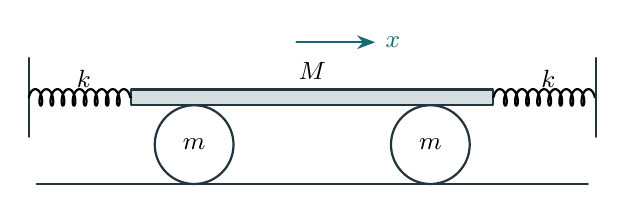
\begin{tikzpicture}[line cap=round,line join=round,spring/.style={decorate,decoration={coil,aspect=.45,segment length=4pt,amplitude=3pt},thick}]\draw[object] (-2,-.5)--(5,-.5);\draw[object] (0,0) circle (.5);\draw[object] (3,0) circle (.5);\draw[object,fill=rulegray] (-.8,.5) rectangle (3.8,.7);\node[above] at (1.5,.7) {$M$};\draw[object](-2.1,.1)--(-2.1,1.1);\draw[spring](-2.1,.6)--(-.8,.6);\draw[spring](3.8,.6)--(5.1,.6);\draw[object](5.1,.1)--(5.1,1.1);\node[above] at (-1.4,.6) {$k$};\node[above] at (4.5,.6) {$k$};\node at (0,0) {$m$};\node at (3,0) {$m$};\draw[motion] (1.3,1.3)--(2.3,1.3) node[right] {$x$};\end{tikzpicture}\figcaption{图 7.13}\end{minipage}\end{center}

\Needspace{18\baselineskip}\subsection*{解答}

\begin{center}\begin{minipage}{\linewidth}\centering\begin{tikzpicture}[font=\small]
\draw[object](-1.2,-.6)--(2,-.6);\draw[object](0,0)circle(.6);
\draw[object,fill=rulegray](-1.2,.6)rectangle(2,.8);
\fill(0,-.6)circle(1pt)node[below]{$P:v_P=0$};
\fill(0,.6)circle(1pt)node[above left]{$Q$};\node at(-.25,.22){$m$};
\draw[motion](0,0)--(.7,0)node[midway,below]{$v_C$};
\draw[motion](0,1.1)--(1.4,1.1)node[midway,above]{$v_Q=2v_C$};
\draw[guide](0,.6)--(0,1.1);\node at(.4,-1.35){$M_{\rm eff}=M+m,\quad H=0$（薄壁筒）};
\end{tikzpicture}\figcaption{解图 7.13A\quad 一个代表圆筒的接触点速度；另一个圆筒具有相同运动。}\end{minipage}\end{center}
令上方物体平衡位移为 $x$，速度 $v=\dot x$；两个圆筒各有质心速度 $v_C$ 和自旋角速度大小 $\omega_r$。底面不滑给 $v_C=r\omega_r$，顶面也不滑给
\[v=v_C+r\omega_r=2v_C,\qquad a_C=\ddot x/2.\]
解图7.13A中的顶点速度是筒心速度的两倍。令物体给每筒的顶面摩擦为 $F$ 向右，地面摩擦为 $H$ 向右记号，取顺时针角加速度为正：
\[ma_C=F+H,\qquad I\beta=(F-H)r,\qquad a_C=r\beta.\]
将转动式除以$r$，并用$a_C=r\beta$，得$F-H=Ia_C/r^2$。它与平动式组成两个关于$F,H$的方程：
\[F=\frac12\left(m+\frac I{r^2}\right)a_C,
\qquad H=\frac12\left(m-\frac I{r^2}\right)a_C.\]
解图7.13A中底摩擦为零，由薄壁筒的$I=mr^2$与这两条动力学方程共同给出。顶点速度为质心速度两倍，则来自上下两处分别不滑动的速度叠加，与这个特殊惯量条件无关。

薄壁筒 $I=mr^2$，于是 $F-H=ma_C$，与平移式相减得 $H=0$、$F=ma_C=m\ddot x/2$。物体受反作用 $-2F$，两弹簧合力为 $-2kx$，因此
\[M\ddot x=-2kx-m\ddot x,\qquad
\boxed{\Omega=\sqrt{\frac{2k}{M+m}}.}\]
摩擦是有符号的约束力；$x>0$ 时 $\ddot x<0$，顶面实际摩擦方向与预设箭头相反。
能量另解需区分质心惯量与接触点惯量。用绕心的 $I_C=mr^2$，两筒总动能为
\[K_{
\text{筒}}=2\left[\frac12m(v/2)^2+\frac12mr^2(v/(2r))^2\right]
=\frac12mv^2.\]
物体动能 $Mv^2/2$，两个弹簧总势能 $kx^2$，故
\[E=\frac12(M+m)\dot x^2+kx^2.\]
求导还原同一方程。若改用底点瞬轴惯量 $2mr^2$，其动能项已经同时包含该筒的质心平移和绕心自转。
\subsubsection*{两处不滑动如何给出二倍速度}
解图7.13A单独放大一个代表圆筒，底接触点记为$P$，顶接触点记为$Q$。
质心向右速度为$v_C$，顺时针自旋角速度为$\omega_r$，
两接触点的水平速度分别为
\[
v_P=v_C-r\omega_r=0,\qquad
v_Q=v_C+r\omega_r=\dot x.
\]
相减、相加才得到$r\omega_r=v_C$与$\dot x=2v_C$。
在半径固定且两处约束持续成立时求导，
$a_C=r\beta=\ddot x/2$。
从某一平衡状态量位移，筒心位移为$x/2$，
所以物体相对每个圆筒有$x/2$的位移，接触位置随之改变。

由平移与转动方程相加、相减，
\[
2F=(m+I_C/r^2)a_C,\qquad
2H=(m-I_C/r^2)a_C.
\]
薄壁筒$I_C=mr^2$时，$F=ma_C,H=0$。
这里$F$是物体作用在圆筒上的摩擦，物体所受力为$-F$。
故两个圆筒对物体的合力为$-2F=-m\ddot x$，
代$M\ddot x=-2kx-2F$后，将惯性项移到同侧，
\[
(M+m)\ddot x+2kx=0.
\]
$-m\ddot x$表示圆筒的惯性反作用，与速度耗散无关。

也可对每个圆筒在该瞬间取地面接触点为取矩点。
顶摩擦力臂为$2r$，底摩擦力臂为零，
平行轴定理给$I_P=I_C+mr^2=2mr^2$，因此
\[
2Fr=2mr^2\beta,\quad F=mr\beta=ma_C.
\]
这是同一动力学的另一写法。
瞬轴惯量包含筒心平移的惯性贡献，用它计算的动能就是该筒的完整动能。

\subsubsection*{动能全项与上接触的能量传递}
一个筒的两项动能分别为
\[
K_{C}=\frac12m(\dot x/2)^2=\frac18m\dot x^2,
\quad K_{s}=\frac12mr^2(\dot x/(2r))^2=\frac18m\dot x^2.
\]
相加后再乘两个筒，得到总筒动能$m\dot x^2/2$。
两弹簧一伸一缩，均提供回复，势能是
$kx^2/2+kx^2/2=kx^2$。
所以
\[
\dot E=(M+m)\dot x\ddot x+2kx\dot x
=\dot x[(M+m)\ddot x+2kx]=0.
\]
在转折点由连续性恢复方程。
给定初始位移$x_0$和匹配纯滚的初始速度$u$，
\[
x(t)=x_0\cos\Omega t+\frac u\Omega\sin\Omega t,
\quad A=\sqrt{x_0^2+(u/\Omega)^2}.
\]
每筒初始质心速度取$u/2$，自旋取$u/(2r)$，使两处接触速度匹配。

底点相对地面静止，底摩擦的功率为零。
顶点却随物体移动，作用在单个筒上的顶摩擦功率为
$F\dot x=2Fv_C$，一般不为零；
物体在同一接触处的功率为$-F\dot x$，二者相消。
接触处两个材料点速度相同，两摩擦力的功率大小相等、方向相反，因此摩擦在两个物体之间传递机械能，接触处没有滑动耗散。

\subsubsection*{一般惯量、静摩擦与接触范围}
令$I_C=\kappa mr^2$，则
\[
F=\frac{m(1+\kappa)}4\ddot x,\quad
H=\frac{m(1-\kappa)}4\ddot x,
\quad M_{\rm eff}=M+\frac{m(1+\kappa)}2.
\]
两筒总动能为$m(1+\kappa)\dot x^2/4$，
所以$\Omega^2=2k/M_{\rm eff}$。
薄壁筒与实心筒分别取$\kappa=1,1/2$；
实心筒的底摩擦随加速度变化，由静摩擦维持底点相对地面静止。

若第$j$个上接触法向力为$N_j$，它的地面法向力为$mg+N_j$，
则每处接触满足
\[
N_j>0,\quad |F|\le\mu_{\text{上}}N_j,
\qquad |H|\le\mu_{\text{地}}(mg+N_j).
\]
$N_1+N_2=Mg$给总支持力；各处的分担还由板的转动平衡确定。
例如上方取不转动的均匀薄板，两筒初始对称、间距为$d$，
薄板质心移动$x$而两筒只移$x/2$，竖直力矩给
\[
N_{1,2}=\frac{Mg}{2}(1\mp x/d).
\]
接触要求$A<d$；薄壁筒所需顶摩擦为$mk|x|/(M+m)$，
在最小支持力的一端还满足
\[
\frac{mkA}{M+m}\le\mu_{\text{上}}\frac{Mg}{2}(1-A/d).
\]
若薄板长为$B$，两接触始终位于板底还要求$B>d+A$。
这些条件给出持续纯滚的振幅范围；滑动阶段则将板位移、筒心位移与转角分别列入动力学方程。


\Needspace{18\baselineskip}

\pdfbookmark[2]{第 14 题 旋转圆盘导轨中弹簧小球的振动}{q14}

\section*{第 14 题\quad 旋转圆盘导轨中弹簧小球的振动}

\tagline{M-07-14}

如图,圆盘绕通过中心O点的竖直轴在水平面内匀速转动,角速度为\(\omega\),质量为\(m\)的小球被约束在圆盘上的光滑导轨AB内运动.小球与劲度系数为\(k\)的弹簧相连(\(k>m\omega^{2}\)),弹簧另一端固定在圆盘A点.弹簧为原长时,小球位于\(P\)点,\(OP=r_{0}\),且\(OP\perp AB\),将小球从\(P\)点沿导轨拉开距离\(a\)后从静止释放.在圆盘参考系中考察小球的运动.

试求小球的平衡位置. 2. 试证明小球作简谐振动, 并求圆频率. 3.
试求导轨施于小球的水平力随时间的变化规律. 4. 试问当 \(k<m \omega^{2}\)
时小球怎样运动.

\begin{center}\begin{minipage}{\linewidth}\centering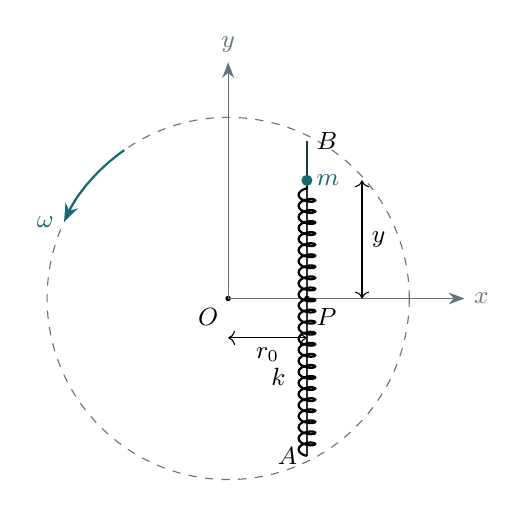
\begin{tikzpicture}[font=\small,spring/.style={decorate,decoration={coil,aspect=.45,segment length=4pt,amplitude=3pt},thick}]
\draw[guide](0,0)circle(2.3);\fill(0,0)circle(1pt)node[below left]{$O$};
\draw[axis](0,0)--(3,0)node[right]{$x$};\draw[axis](0,0)--(0,3)node[above]{$y$};
\draw[object](1,-2)--(1,2);\draw[spring](1,-2)--(1,1.5);
\node[left]at(1,-2){$A$};\fill(1,0)circle(1pt)node[below right]{$P$};\node[right]at(1,2){$B$};
\fill[accent](1,1.5)circle(2pt)node[right]{$m$};\node[left]at(.85,-1){$k$};
\draw[<->](0,-.5)--(1,-.5)node[midway,below]{$r_0$};
\draw[<->](1.7,0)--(1.7,1.5)node[midway,right]{$y$};
\draw[motion](-1.319225804,1.884049702)arc(125:155:2.3)node[left]{$\omega$};
\end{tikzpicture}\figcaption{图 7.14}\end{minipage}\end{center}

\Needspace{18\baselineskip}\subsection*{解答}

\begin{center}\begin{minipage}{\linewidth}\centering\begin{tikzpicture}[font=\small,spring/.style={decorate,decoration={coil,aspect=.45,segment length=4pt,amplitude=3pt},thick}]
\draw[guide](0,0)circle(2.3);\fill(0,0)circle(1pt)node[below left]{$O$};
\draw[axis](0,0)--(3,0)node[right]{$x$};\draw[axis](0,0)--(0,3)node[above]{$y$};
\draw[object](1,-2)--(1,2);\draw[spring](1,-2)--(1,1.5);
\node[left]at(1,-2){$A$};\fill(1,0)circle(1pt)node[below right]{$P$};\node[left]at(1,2){$B$};
\fill[accent](1,1.5)circle(2pt)node[right]{$m$};\node[left]at(.85,-1){$k$};
\draw[<->](0,-.5)--(1,-.5)node[midway,below]{$r_0$};
\draw[<->](1.7,0)--(1.7,1.5)node[midway,right]{$y$};
\draw[motion](-1.319225804,1.884049702)arc(125:155:2.3)node[left]{$\omega$};

\draw[force](1,1.5)--(1,-.3)node[midway,left]{$-ky$};
\draw[force](1,1.5)--(.4,1.5)node[above left]{$N_x$};
\draw[force](1,1.5)--(1.6,2.4)node[right]{$m\omega^2\boldsymbol r$};
\node at(.4,-2.8){释放瞬间：$\dot y=0$，图示$k=2m\omega^2$};
\end{tikzpicture}\figcaption{解图 7.14A}\end{minipage}\end{center}
在盘面坐标中取 $x$ 沿 $OP$、$y$ 沿导轨，$\boldsymbol\omega=\omega\hat{\boldsymbol z}$。小球位置为 $(r_0,y)$，相对速度为 $\dot y\hat{\boldsymbol y}$。离心力为 $m\omega^2(r_0\hat{\boldsymbol x}+y\hat{\boldsymbol y})$；科里奥利力为 $2m\omega\dot y\hat{\boldsymbol x}$。导轨水平力记为有符号的 $N_x$，分量式为
\[N_x+m\omega^2r_0+2m\omega\dot y=0,
\quad N_z=mg,\quad m\ddot y=-(k-m\omega^2)y.\]
科里奥利方向可直接由叉乘给出：$\hat{\boldsymbol z}\times\hat{\boldsymbol y}=-\hat{\boldsymbol x}$，所以$-2m\boldsymbol\omega\times\boldsymbol v_{\rm rel}$的有符号分量为$2m\omega\dot y$；$\dot y>0$时指向$+x$，$\dot y<0$时指向$-x$。它沿导轨的投影为零，导轨的侧向力抵消它与离心力的横向分量之和。离心力的$y$分量却为$m\omega^2y$，与偏离同向，会抵消一部分弹簧回复；这就是解图7.14A中沿轨稳定性由$k-m\omega^2$决定的原因。

当 $k>m\omega^2$，平衡位于 $P$，即 $y=0$，回复系数为 $k-m\omega^2>0$。由 $y(0)=a,\dot y(0)=0$，
\[\boxed{y=a\cos\Omega t,\quad\Omega=\sqrt{k/m-\omega^2},\quad
N_x=2am\omega\Omega\sin\Omega t-m\omega^2r_0.}\]
双侧槽中，侧向力由正变负时，施力面从一侧转到另一侧。
当 $k=m\omega^2$ 时回复系数为零，$\ddot y=0$。所给零初速使 $y=a$ 保持不变；一般初速则匀速漂移，并无振动周期。
当 $k<m\omega^2$，令 $\lambda=\sqrt{\omega^2-k/m}$，运动方程为 $\ddot y=\lambda^2y$。乘 $\dot y$ 积分：
\[\dot y^2=\lambda^2y^2+C,\quad C=-\lambda^2a^2,
\quad\int_a^y\frac{\dd Y}{\sqrt{Y^2-a^2}}=\lambda t.\]
对 $a>0,t\ge0$ 取外移支，积分为 $\operatorname{arcosh}(y/a)=\lambda t$，故
\[\boxed{y=a\cosh\lambda t,\quad
N_x=-m\omega^2r_0-2m\omega a\lambda\sinh\lambda t.}\]
若 $a<0$，同一个双曲余弦解向负方向离开平衡；有限导轨只允许该解用到碰到端点之前。科里奥利力垂直导轨运动，不改变沿轨频率，却决定侧向压力。
\subsubsection*{盘系横坐标与地面横向加速度}
解图7.14A取释放瞬间$\dot y=0$，科里奥利力暂为零。
图中$N_x$向$O$一侧，抵消离心力的$x$分量，
沿轨弹力和离心力之差决定释放加速度。
对一般时刻先逐项写出
\[
\boldsymbol F_{\text{离}}=m\omega^2(r_0\hat{\boldsymbol x}+y\hat{\boldsymbol y}),
\quad\boldsymbol F_{\rm Cor}=2m\omega\dot y\hat{\boldsymbol x}.
\]
盘系的$x$不变，所以相对$x$加速度为零，才有
$N_x=-m\omega^2r_0-2m\omega\dot y$。
这里为零的是相对加速度的横向分量，地面加速度还须计入坐标轴转动。

地面系写法直接给出真实水平力。将盘系位置$(r_0,y)$旋转$\omega t$后求两次导数，
再把加速度投回盘系，得到
\[
a_{{\text{地}},x}=-\omega^2r_0-2\omega\dot y,
\qquad a_{{\text{地}},y}=\ddot y-\omega^2y.
\]
真实水平力只有$N_x\hat{\boldsymbol x}-ky\hat{\boldsymbol y}$，
因此$N_x=ma_{{\text{地}},x}$、$-ky=ma_{{\text{地}},y}$，
恢复同一侧向力和沿轨方程。

\subsubsection*{平衡、初值与三种有效刚度}
沿轨平衡条件是$(k-m\omega^2)y=0$。
若$k\ne m\omega^2$，唯一平衡在$P$；
正刚度时稳定，负刚度时仍是平衡位置但不稳定。
临界值$k=m\omega^2$时，每个允许的$y$都可相对圆盘静止，
只是没有回复作用，给定非零速度便沿轨漂移。

稳定情形取$\Omega^2=k/m-\omega^2>0$。
通解$y=C\cos\Omega t+D\sin\Omega t$中，
$C=a,\Omega D=0$，故$y=a\cos\Omega t$。
求导再代侧向式，
\[
\dot y=-a\Omega\sin\Omega t,
\quad N_x=-m\omega^2r_0+2ma\omega\Omega\sin\Omega t.
\]
释放端点处速度项为零；过$P$的两次速率同大，
速度方向相反，所以侧向力也分别取两个不同极值。

失稳情形取$\lambda^2=\omega^2-k/m>0$。
从静止释放的第一次积分为
\[
\frac12\dot y^2-\frac12\lambda^2y^2=-\frac12\lambda^2a^2.
\]
对$a>0,t>0$，初始加速度$\lambda^2a>0$，
故应选正的外移支$\dot y=\lambda\sqrt{y^2-a^2}$。
令$Y=a\cosh s$，则$\dd Y=a\sinh s\dd s$、
$\sqrt{Y^2-a^2}=a\sinh s$，积分直接给$s=\lambda t$。
于是$y=a\cosh\lambda t$；$a<0$时向负侧离开。
若$a=0$且初速度也零，这组初值给恒定解$y=0$，对应不稳定平衡。

\begin{center}\begin{minipage}{\linewidth}\centering
\begin{tikzpicture}[font=\small,x=3cm,y=.9cm]
\draw[axis](0,0)--(2.2,0)node[right]{$\tau=\nu t$};
\draw[axis](0,-.5)--(0,3.6)node[above]{$y/a$};
\draw[traj,domain=0:1.8,samples=81]plot(\x,{cos(deg(\x))});
\draw[guide](0,1)--(1.8,1);
\draw[object,domain=0:1.8,samples=81]plot(\x,{(exp(\x)+exp(-\x))/2});
\node[left]at(0,1){$1$};\node[right]at(1.8,-.227202095){稳定};
\node[right]at(1.8,1){临界，零初速};\node[right]at(1.8,3.107473176){失稳};
\node[below left]at(0,0){$0$};
\end{tikzpicture}
\figcaption{解图7.14B\quad 取$0<\nu<\omega$，分别令$k/m-\omega^2=\nu^2,0,-\nu^2$，三种零初速运动由同一$y(0)=a>0$开始。}
\end{minipage}\end{center}
若另给初速度$u$，三类解分别为
\[
\begin{aligned}
y&=a\cos\Omega t+(u/\Omega)\sin\Omega t,&&k>m\omega^2,\\
y&=a+ut,&&k=m\omega^2,\\
y&=a\cosh\lambda t+(u/\lambda)\sinh\lambda t,&&k<m\omega^2.
\end{aligned}
\]
失稳方程含增长、衰减两个指数分量；
特选$u=-\lambda a$会消去增长分量，只留下沿衰减方向的运动。
极小的增长分量仍会随时间放大。

\subsubsection*{侧向力极值、单侧导轨与可用时间}
在$\omega>0,r_0\ge0$的稳定情形，
\[
N_{x,\min}=-m\omega^2r_0-2m\omega|a|\Omega,
\quad N_{x,\max}=-m\omega^2r_0+2m\omega|a|\Omega.
\]
真正变号要求$2|a|\Omega>\omega r_0$；
等号时最大值触零，整个周期的反力仍为非正。
双侧光滑槽可承担两种符号。
若仅允许向$-x$施压，整周期可行的条件为
$2|a|\Omega\le\omega r_0$；
仅允许向$+x$施压且$r_0>0$时，负的平均值已排除整周期运动。

有限导轨上的完整振动取振幅小于$PA$和$PB$，使球留在两端之间、弹簧保持正长度。
若失稳向正侧、$PB=b>a>0$，模型只适用到
\[
t_{\text{端}}=\lambda^{-1}\operatorname{arcosh}(b/a).
\]
到端点的时刻给出这段双曲余弦运动的终点。

\subsubsection*{有效能量与维持匀速转盘的功}
将沿轨方程乘$\dot y$，得
\[
\mathcal E=\frac12m\dot y^2+\frac12(k-m\omega^2)y^2=\text{常量}.
\]
它的势能曲率直接区分稳定、临界和失稳。
地面系机械能还包含转盘带来的运动：
真实地面速度在盘面方向的分量为$(-\omega y,\dot y+\omega r_0)$，故
\[
E_{\text{地}}=\frac m2[\omega^2y^2+(\dot y+\omega r_0)^2]+\frac12ky^2.
\]
地面角动量为$L_z=m[r_0\dot y+\omega(r_0^2+y^2)]$，
相减给
\[
E_{\text{地}}-\omega L_z=\mathcal E-\frac12m\omega^2r_0^2.
\]
因此$\dot E_{\text{地}}=\omega\dot L_z$，
维持圆盘匀速的装置与小球、弹簧交换机械能。
科里奥利力垂直相对速度，故相对运动有上式的有效能量常量；地面机械能的变化率由转动力矩给定。


\Needspace{18\baselineskip}

\pdfbookmark[2]{第 15 题 圆周弹簧质点受径向轻击后的径向频率}{q15}

\section*{第 15 题\quad 圆周弹簧质点受径向轻击后的径向频率}

\tagline{M-07-15}

如图,质量为\(m\)的小球在光滑水平桌面上以角速度\(\omega\)作匀速圆周运动.所需的向心力由与小球相连的弹簧提供,弹簧的劲度系数为\(k\),另一端固定.今沿径向轻击小球.试求小球径向振动的频率.

\begin{center}\begin{minipage}{\linewidth}\centering\begin{tikzpicture}[font=\small,spring/.style={decorate,decoration={coil,aspect=.45,segment length=4pt,amplitude=3pt},thick}]
\draw[guide](0,0)circle(2);\fill(0,0)circle(1.2pt)node[below left]{$O$};
\draw[spring](0,0)--(2,0);\fill[accent](2,0)circle(2pt)node[below right]{$m$};
\draw[motion](2,0)--(2,.85)node[right]{$R\omega$};
\draw[force](2,0)--(2.9,0)node[right]{$J_r$（径向）};
\draw[<->](0,-.65)--(1.2,-.65)node[midway,below]{$r_0$};
\draw[<->](0,-1.25)--(2,-1.25)node[midway,below]{$R$};
\end{tikzpicture}\figcaption{图 7.15}\end{minipage}\end{center}

\Needspace{18\baselineskip}\subsection*{解答}

\begin{center}\begin{minipage}{\linewidth}\centering\begin{tikzpicture}[font=\small,spring/.style={decorate,decoration={coil,aspect=.45,segment length=4pt,amplitude=3pt},thick}]
\draw[guide](0,0)circle(2);\fill(0,0)circle(1.2pt)node[above left]{$O$};
\draw[spring](0,0)--(2.3,0);\fill[accent](2.3,0)circle(2pt)node[below right]{$m$};
\draw[motion](2.3,0)--(2.3,.739130435)node[right]{$r\dot\varphi$};
\draw[motion](2.3,0)--(3,0)node[right]{$\dot r$};
\draw[guide](2,-.3)--(2,.25);\draw[<->](2,-.35)--(2.3,-.35)node[midway,below]{$\delta$};
\draw[<->](0,-.85)--(1.2,-.85)node[midway,below]{$r_0$};
\draw[<->](0,-1.45)--(2.3,-1.45)node[midway,below]{$r=R+\delta$};
\node at(.5,-2.6){$L=mr^2\dot\varphi=mR^2\omega$；虚圆为未扰动半径$R$};
\end{tikzpicture}\figcaption{解图 7.15A}\end{minipage}\end{center}
分别以 $r_0$、$R$、$r$ 表示弹簧原长、未扰动圆轨道半径、扰动后的距离。圆轨道平衡满足
\[k(R-r_0)=mR\omega^2.\]
径向轻击不改变绕 $O$ 的角动量，$L=mr^2\dot\varphi=mR^2\omega$。径向运动方程为
\[m\ddot r=\frac{L^2}{mr^3}-k(r-r_0).\]
令 $\delta=r-R$，利用 $(1+\delta/R)^{-3}=1-3\delta/R+O(\delta^2/R^2)$，则
\[m\ddot\delta=mR\omega^2\left(1-3\delta/R\right)-k(R-r_0)-k\delta
=-(k+3m\omega^2)\delta.\]
平衡常数项相消，得
\[\boxed{\Omega_r=\sqrt{k/m+3\omega^2},\qquad
\nu_r=\frac{\Omega_r}{2\pi}.}\]
解图7.15A显示半径增大时角速度降为 $R^2\omega/r^2$；沿径向往复的每一时刻均用$r^2\dot\varphi=R^2\omega$确定角速度。若初始纯径向小冲量给径向速度 $u$，则 $\delta(0)=0$、$\dot\delta(0)=u$，所以 $\delta=(u/\Omega_r)\sin\Omega_rt$。
径向冲量只给径向速度，故碰后瞬间角动量不变。线性解的振幅为$|u|/\Omega_r$，取$|u|/(R\Omega_r)\ll1$，并使弹簧在整个径向振幅内保持线性伸缩。将角速度按同一小量展开
\[\dot\varphi=\omega\frac{R^2}{(R+\delta)^2}
\simeq\omega\left(1-\frac{2\delta}{R}\right).\]
半径变大时切向角速度下降，角动量约束因此使径向回复中多出$3m\omega^2$；这项回复来自切向运动随半径重新分配。

有效势能 $U_{
\rm eff}=L^2/(2mr^2)+k(r-r_0)^2/2$ 在 $R$ 处的二阶导数为 $k+3m\omega^2$，给相同判据。圆轨道的存在还要求 $k>m\omega^2$（$r_0>0$ 时）；这与扰动后的正回复曲率是两个条件。
\subsubsection*{三个半径和圆轨道存在条件}
图7.15把弹簧自然长标为$r_0$，未扰动圆半径标为$R$；
切向速度由圆轨道半径给出，为$R\omega$。
弹簧力提供向心力时，$R-r_0>0$，平衡式可整理为
\[
(k-m\omega^2)R=kr_0,\qquad
R=\frac{kr_0}{k-m\omega^2}.
\]
若$r_0>0$，有限正圆轨道对应$k>m\omega^2$。
当转速接近$\sqrt{k/m}$，这个半径趋于无穷；
在这一极限中，$R$随转速一起增大。
若$r_0=0$，平衡式化为$(k-m\omega^2)R=0$；取$R>0$得$\omega^2=k/m$，
此时任何正的$R$都满足力学平衡。

径向冲量$J_r$与位置矢量共线，其冲量矩为零，
故轻击前后角动量相同，径向速度增加$u=J_r/m$。
轻击瞬间切向速度仍是$R\omega$；新增的径向速度使机械能增加$mu^2/2$。
解图7.15A画的是轻击后$r=R+\delta$的时刻，
虚圆为未扰动轨道，球与虚圆之间的径向距离由$\delta$标出。

\subsubsection*{负三次幂及平衡消项的全计算}
将$L=mR^2\omega$代入径向式，
\[
\ddot\delta=\frac{R^4\omega^2}{(R+\delta)^3}
-\frac{k}{m}(R+\delta-r_0)
=R\omega^2(1+\delta/R)^{-3}
-\frac{k}{m}(R-r_0)-\frac{k}{m}\delta.
\]
这里固定的是$L$，因而外向项的分母为三次幂。
展开到所需阶，
\[
\ddot\delta=
\underbrace{R\omega^2-\frac{k}{m}(R-r_0)}_{=0}
-\left(3\omega^2+\frac{k}{m}\right)\delta
+\frac{6\omega^2}{R}\delta^2+O(\delta^3/R^2).
\]
二次项说明有限幅运动不再严格简谐，
线性角频率才是$\Omega_r=\sqrt{k/m+3\omega^2}$。
普通频率为$\nu_r=\Omega_r/(2\pi)$。
由冲量初值，径向振幅$A_r=|J_r|/(m\Omega_r)$，
要求$A_r/R\ll1$；若弹簧只能受拉，还须$A_r<R-r_0$，
使线性估计的整个运动不进入压缩或松弛区。

\subsubsection*{有效势、能量与角度变化}
真实机械能可写成
\[
E=\frac12m\dot r^2+U_{\rm eff}(r),\quad
U_{\rm eff}=\frac{L^2}{2mr^2}+\frac12k(r-r_0)^2.
\]
有效势的第一项就是按角动量改写的切向动能。
对半径分别求导，
\[
U'=-\frac{L^2}{mr^3}+k(r-r_0),\quad
U''=\frac{3L^2}{mr^4}+k>0.
\]
圆轨道先由$U'(R)=0$确定，
再由$U''(R)=k+3m\omega^2>0$得稳定圆轨道，
曲率除以$m$恢复同一$\Omega_r^2$。
轻击后能量为$U_{\rm eff}(R)+mu^2/2$，
两个径向转折点由$U_{\rm eff}(r)=E$求得；
它们只在线性近似下关于$R$等距。
对于只受拉的连接，$E<U_{\rm eff}(r_0)$使内端转折点位于自然长外侧。

角速度的一阶变化须与径向解同步。
当$\delta=(u/\Omega_r)\sin\Omega_rt$、$\varphi(0)=0$时，
\[
\dot\varphi\simeq\omega\left(1-\frac{2\delta}{R}\right),\qquad
\varphi(t)\simeq\omega t+
\frac{2\omega u}{R\Omega_r^2}(\cos\Omega_rt-1).
\]
每次径向往复期间，小球仍绕$O$转动。
在线性阶，每个径向周期内的方位增量为
$2\pi\omega/\Omega_r$。
若$r_0>0$且$\omega>0$，存在条件还给$\Omega_r>2\omega$；
自然长为零时才取等号。

自然长为零时，地面直角坐标给出完整轨迹。
取$\omega^2=k/m$，轻击后的地面坐标精确为
\[
X=R\cos\omega t+(u/\omega)\sin\omega t,\qquad
Y=R\sin\omega t.
\]
两坐标都满足同一线性谐振方程。
非零径向冲量使$r^2=X^2+Y^2$出现角频率$2\omega$的变化，因此径向周期为$\pi/\omega$；
实际半径为 $r=\sqrt{X^2+Y^2}$，对有限冲量应保留这个平方根。小冲量时将它展开到一阶，才得到角频率 $2\omega$ 的正弦变化。


\Needspace{18\baselineskip}

\pdfbookmark[2]{第 16 题 有限振幅单摆周期的二级近似}{q16}

\section*{第 16 题\quad 有限振幅单摆周期的二级近似}

\tagline{M-07-16}

计算单摆周期时,若摆幅 \(\theta_{0}\) 较小,可采用一级近似
\(\sin \theta \approx \theta\),算出的周期为
\(T_{0}=2 \pi \sqrt{\frac{l}{g}}\),其中 \(l\) 为摆长.若 \(\theta_{0}\)
不算小,就应取二级近似.试导出单摆周期 \(T\) 与摆幅 \(\theta_{0}\) 的关系.

\begin{center}\begin{minipage}{\linewidth}\centering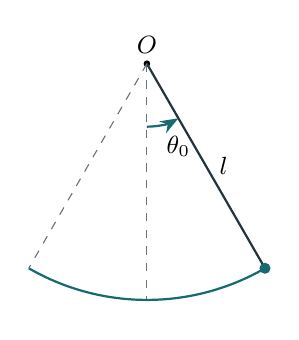
\begin{tikzpicture}[font=\small]
\fill(0,0)circle(1.2pt)node[above]{$O$};
\draw[object](0,0)--(1.5,-2.598076211);\fill[accent](1.5,-2.598076211)circle(2pt);
\draw[guide](0,0)--(0,-3);\draw[guide](0,0)--(-1.5,-2.598076211);
\draw[traj](-1.5,-2.598076211)arc(-120:-60:3);
\draw[motion](0,-.8)arc(-90:-60:.8);\node at(.4,-1.05){$\theta_0$};
\node[right]at(.8,-1.3){$l$};
\end{tikzpicture}\figcaption{图 7.16}\end{minipage}\end{center}

\Needspace{18\baselineskip}\subsection*{解答}

\begin{center}\begin{minipage}{\linewidth}\centering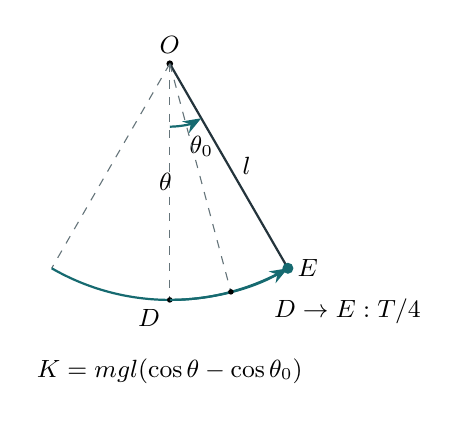
\begin{tikzpicture}[font=\small]
\fill(0,0)circle(1.2pt)node[above]{$O$};
\draw[object](0,0)--(1.5,-2.598076211);\fill[accent](1.5,-2.598076211)circle(2pt);
\draw[guide](0,0)--(0,-3);\draw[guide](0,0)--(-1.5,-2.598076211);
\draw[traj](-1.5,-2.598076211)arc(-120:-60:3);
\draw[motion](0,-.8)arc(-90:-60:.8);\node at(.4,-1.05){$\theta_0$};
\node[right]at(.8,-1.3){$l$};

\fill(0,-3)circle(1pt)node[below left]{$D$};\node[right]at(1.5,-2.598076211){$E$};
\draw[motion](0,-3)arc(-90:-60:3);\node[right]at(1.2,-3.15){$D\to E:T/4$};
\draw[guide](0,0)--(.776457135,-2.897777479);\fill(.776457135,-2.897777479)circle(1pt);
\node[left]at(.15,-1.5){$\theta$};
\node at(0,-3.9){$K=mgl(\cos\theta-\cos\theta_0)$};
\end{tikzpicture}\figcaption{解图 7.16A}\end{minipage}\end{center}
先采用固定摆长的理想模型，设$0<\theta_0<\pi$，最大摆角处速度为零。由机械能守恒，
\[\frac12ml^2\dot\theta^2+mgl(1-\cos\theta)
=mgl(1-\cos\theta_0),\]
故 $|\dot\theta|=\sqrt{2g/l}\sqrt{\cos\theta-\cos\theta_0}$。从零角走到端点是四分之一周期，取速率作积分：
\[\frac T4=\sqrt{\frac l{2g}}\int_0^{\theta_0}
\frac{\dd\theta}{\sqrt{\cos\theta-\cos\theta_0}}.\]
解图7.16A标出积分的一段，四段由对称性补全。令 $s=\sin(\theta_0/2)$、$\sin(\theta/2)=s\sin\phi$，则
\[\dd\theta=\frac{2s\cos\phi}{\sqrt{1-s^2\sin^2\phi}}\dd\phi,
\quad\cos\theta-\cos\theta_0=2s^2\cos^2\phi.\]
将端点从 $\theta=0,\theta_0$ 变成 $\phi=0,\pi/2$，得到无端点奇异性的形式
\[T=4\sqrt{l/g}\int_0^{\pi/2}\frac{\dd\phi}{\sqrt{1-s^2\sin^2\phi}}.\]
\Needspace{13\baselineskip}当摆幅适度，保留 $\theta_0^2$ 项：
\[(1-s^2\sin^2\phi)^{-1/2}=1+\frac{s^2}{2}\sin^2\phi+O(s^4),
\quad s^2=\theta_0^2/4+O(\theta_0^4).\]
利用 $\int_0^{\pi/2}\sin^2\phi\dd\phi=\pi/4$，可得
\[\boxed{T=T_0\left[1+\frac{\theta_0^2}{16}+O(\theta_0^4)\right],
\qquad T_0=2\pi\sqrt{l/g}.}\]
上述二级系数可直接从积分逐步看出：
\[\frac{T}{T_0}=\frac2\pi\left(\frac\pi2+
\frac{s^2}{2}\frac\pi4+O(s^4)\right)
=1+\frac{s^2}{4}+O(s^4)
=1+\frac{\theta_0^2}{16}+O(\theta_0^4).\]
它必为正修正：$\sin\theta<\theta$意味着真实回复力弱于同角度的线性模型，摆走完整条弧所需时间更长。求四阶项时，保留被积式的$3s^4\sin^4\phi/8$，并用
\[\int_0^{\pi/2}\sin^4\phi\dd\phi=\frac{3\pi}{16},
\qquad s^2=\frac{\theta_0^2}{4}-\frac{\theta_0^4}{48}+O(\theta_0^6),\]
便有$T/T_0=1+s^2/4+9s^4/64+\cdots$，四次项为$-1/192+9/1024=11/3072$。解图7.16A的端点虽速度为零，原时间积分仍收敛；新变量把这个可积奇点消去了。

级数中的角度用弧度。$2.5^\circ=0.043633\,\mathrm{rad}$ 时，相对增加约 $1.19\times10^{-4}$。接近竖直向上的分离轨道时，使用完整周期积分；当$\theta_0\to\pi$，周期呈对数增长。
\subsubsection*{四分之一周期与换元中的正负号}
解图7.16A以最低点$D$到右端点$E$为积分弧。
从$D$向$E$的角速度为正，从$E$返回$D$则为负，
两段所需时间相同。能量先给角速度的平方，
取出程的正速率积分，回程按相同的弧长和速率计时。
由$\cos\theta-\cos\theta_0=
2[\sin^2(\theta_0/2)-\sin^2(\theta/2)]$，
四分之一周期可写成
\[
\frac T4=\frac12\sqrt{\frac lg}
\int_0^{\theta_0}\frac{\dd\theta}{\sqrt{s^2-\sin^2(\theta/2)}},
\quad s=\sin(\theta_0/2).
\]
换元$\sin(\theta/2)=s\sin\phi$时，$s$是常数，
\[
\frac12\cos(\theta/2)\dd\theta=s\cos\phi\dd\phi,
\quad \cos(\theta/2)=\sqrt{1-s^2\sin^2\phi}>0.
\]
在$0\le\phi\le\pi/2$有$\cos\phi\ge0$，
所以分母的$\sqrt{s^2\cos^2\phi}=s\cos\phi$，
与微分中的同因子相消，没有额外负号。
这里的$1/2$与微分中的2相消，最后乘四个等时段，
才得到$T=4\sqrt{l/g}\int_0^{\pi/2}(1-s^2\sin^2\phi)^{-1/2}\dd\phi$。

\subsubsection*{按同一小参数计阶和定量误差}
二阶近似指周期保留到幅值的平方阶。运动方程中的$\sin\theta$为奇函数，其首个非线性项为$-\theta^3/6$。
在固定积分区间内，取
\[
(1-q)^{-1/2}=1+\frac q2+\frac{3q^2}{8}+\cdots,
\qquad q=s^2\sin^2\phi.
\]
因$s=\theta_0/2+O(\theta_0^3)$，
$q$是幅值二阶，而$q^2$是幅值四阶。
只求二阶时，$s^2$用$\theta_0^2/4$已足够；
四阶系数由$s^2/4$的$-\theta_0^4/192$与$9s^4/64$的$9\theta_0^4/1024$相加得到。

以精确的积分数值作比较，定义
$T_2/T_0=1+\theta_0^2/16$、
$T_4/T_0=1+\theta_0^2/16+11\theta_0^4/3072$，有
\begin{center}\begin{tabular}{r|rrr}
$\theta_0$&精确积分$T/T_0$&$T_2/T_0$&$T_4/T_0$\\\hline
$2.5^\circ$&1.000119004&1.000118991&1.000119004\\
$5^\circ$&1.000476172&1.000475965&1.000476172\\
$30^\circ$&1.017408798&1.017134730&1.017403862\\
$60^\circ$&1.073182007&1.068538919&1.072845038\\
$90^\circ$&1.180340599&1.154212569&1.176012292\\
\end{tabular}\end{center}
表中区分了两种误差：小角式$T_0$遗漏的有限幅修正，
与二阶式$T_2$相对于精确周期的截断误差。
$2.5^\circ$时前者约$1.19\times10^{-4}$，
后者只有约$1.30\times10^{-8}$；报告误差时应注明采用哪个周期作比较。
$60^\circ$时二阶式对精确周期的相对误差已约$0.433\%$，
$90^\circ$时约$2.21\%$，可按所需精度选二阶、四阶或完整周期积分。

若只用$T_0$而要求相对修正小于$\varepsilon$，
平方阶估计给$\theta_0\lesssim4\sqrt\varepsilon$。
例如$\varepsilon=10^{-3}$，阈值约$7.25^\circ$。
这是二阶角幅估计；给定严格误差上限时，将完整周期积分与该上限联立求角幅。
摆长只乘在共同时间因子上，不改变相对修正；
绝对时间差$T-T_0$仍随$\sqrt l$变化。

\subsubsection*{普通端点、近顶端和细线的拉力条件}
固定$0<\theta_0<\pi$，令$\epsilon=\theta_0-\theta$，
\[
\cos\theta-\cos\theta_0=\sin\theta_0\,\epsilon+O(\epsilon^2).
\]
所以端点附近$\dd t$正比$\dd\epsilon/\sqrt\epsilon$，
这个端点积分收敛，所以摆球在有限时间到达普通转折点，速率在那里降为零。
但当$\theta_0\to\pi$，半角积分中的
$\sqrt{1-s^2\sin^2\phi}$在$\phi\to\pi/2$变小。
令$q=\pi/2-\phi$，局部分母近似
$\sqrt{\cos^2(\theta_0/2)+q^2}$，
其积分呈对数增长，故周期发散。
二阶或四阶多项式在$\theta_0=\pi$仍有限，正说明它们在该极限已经失效。

上述接近顶端的讨论采用固定摆长、可维持圆弧的数学模型。
若用只能受拉的细线，并从端点静止释放，张力满足
\[
\mathcal T-mg\cos\theta=ml\dot\theta^2,
\quad\mathcal T(\theta_0)=mg\cos\theta_0.
\]
由能量再代入可得$\mathcal T=mg(3\cos\theta-2\cos\theta_0)$，在往复段的最小值出现在端点。
因此$\theta_0\le\pi/2$既是初始绷紧条件，也保证这段圆弧运动的张力始终非负。
从大于直角的位置静止释放时，细线先松弛；摆球按抛体运动，细线再次绷紧后再转入圆弧运动。
要保持大于直角乃至近$\pi$的固定摆长往复，可采用能承受拉压的轻杆。
所以数学周期积分的角度范围与具体摆线装置的接触约束要分别说明。


\Needspace{18\baselineskip}

\pdfbookmark[2]{第 17 题 谐振子的相积分与能量频率关系}{q17}

\section*{第 17 题\quad 谐振子的相积分与能量频率关系}

\tagline{M-07-17}

对于谐振子,若广义动量为\(p\),广义坐标为\(q\),则有\(\oint p\mathrm{d}q=\frac{E}{\nu}\),其中\(E\)为谐振子的能量,\(\nu\)为振动频率.积分在振动的一个周期内进行.试就弹簧振子和单摆的情况证明此式.

\begin{center}\begin{minipage}{\linewidth}\centering\begin{tikzpicture}[line cap=round,line join=round,spring/.style={decorate,decoration={coil,aspect=.45,segment length=4pt,amplitude=3pt},thick}]\draw[axis] (-2.4,0)--(2.5,0) node[right] {$x$};\draw[axis] (0,-1.7)--(0,1.8) node[above] {$p_x$};\draw[traj] (0,0) ellipse (2 and 1.3);\node at (0,-2.1) {弹簧振子};\begin{scope}[xshift=6cm]\draw[axis] (-2.4,0)--(2.5,0) node[right] {$\theta$};\draw[axis] (0,-1.7)--(0,1.8) node[above] {$p_\theta$};\draw[traj] (0,0) ellipse (2 and 1.3);\node at (0,-2.1) {小角单摆};\end{scope}\end{tikzpicture}\figcaption{图 7.17}\end{minipage}\end{center}

\Needspace{18\baselineskip}\subsection*{解答}

\begin{center}\begin{minipage}{\linewidth}\centering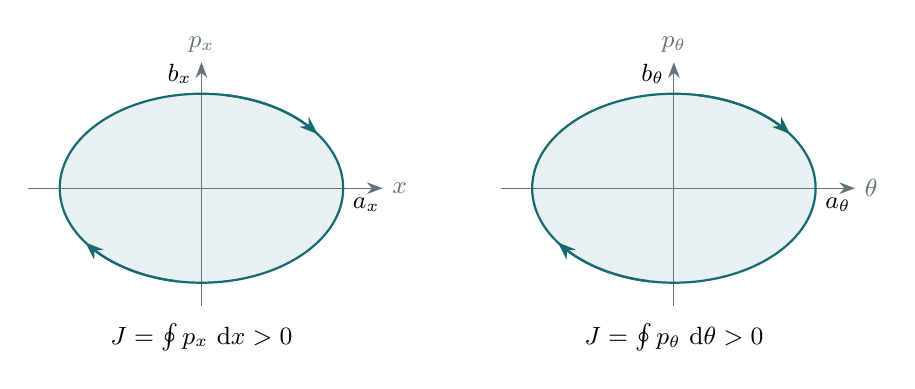
\begin{tikzpicture}[font=\small]
\foreach \sh/\xx/\pp/\aa/\bb in {0/x/p_x/a_x/b_x,6/\theta/p_\theta/a_\theta/b_\theta}{
\begin{scope}[xshift=\sh cm]
\fill[accent!10](0,0)ellipse(1.8 and 1.2);
\draw[axis](-2.2,0)--(2.3,0)node[right]{$\xx$};\draw[axis](0,-1.5)--(0,1.6)node[above]{$\pp$};
\draw[traj](0,0)ellipse(1.8 and 1.2);
\draw[motion,domain=80:35,samples=21]plot({1.8*cos(\x)},{1.2*sin(\x)});
\draw[motion,domain=260:215,samples=21]plot({1.8*cos(\x)},{1.2*sin(\x)});
\node[below right]at(1.8,0){$\aa$};\node[above left]at(0,1.2){$\bb$};
\node at(0,-1.9){$J=\oint\pp\,\dd\xx>0$};
\end{scope}}
\end{tikzpicture}\figcaption{解图 7.17A}\end{minipage}\end{center}
对弹簧振子，$p=m\dot x$，以平衡势能为零，
\[E=\frac{p^2}{2m}+\frac12kx^2,
\qquad\frac{x^2}{2E/k}+\frac{p^2}{2mE}=1.\]
相平面是解图7.17A中的椭圆，半轴为 $a=\sqrt{2E/k}$、$b=\sqrt{2mE}$。沿实际运动一周，$p\dd x$ 的积分等于椭圆正面积：
\[\oint p\dd x=\pi ab=2\pi E\sqrt{m/k}
=\frac{2\pi E}{\Omega}=\frac E\nu,\quad\nu=\frac\Omega{2\pi}.\]
也可显式参数化 $x=A\cos\Omega t$、$p=-mA\Omega\sin\Omega t$，于是
\[\oint p\dd x=mA^2\Omega^2\int_0^T\sin^2\Omega t\dd t
=mA^2\Omega^2T/2=ET.\]
\Needspace{14\baselineskip}单摆在线性近似下，广义坐标为 $\theta$，对应的广义动量为角动量
\[p_\theta=ml^2\dot\theta,\quad
E=\frac{p_\theta^2}{2ml^2}+\frac12mgl\theta^2.\]
它也给椭圆
\[\frac{\theta^2}{2E/(mgl)}+\frac{p_\theta^2}{2ml^2E}=1.\]
两半轴相乘并乘 $\pi$，得到
\[\boxed{\oint p_\theta\dd\theta=2\pi E\sqrt{l/g}=\frac E\nu.}\]
相图中的积分符号由上下两支的运动方向确定。上支$p>0$时质点向右，$\dd x>0$；下支$p<0$时向左，$\dd x<0$，两支的$p\dd x$均为正。故
\[J=2\int_{-A}^{A}\sqrt{2m(E-kx^2/2)}\dd x>0.\]
对$H=p^2/(2m)+U(x)$、质量为常量的一维束缚系统，若转折点为$x_\pm(E)$，求导时端点处$p=0$，移动积分限的端点项为零，于是
\[\frac{\dd J}{\dd E}=2\int_{x_-}^{x_+}\frac{m\,\dd x}{p(x,E)}=T(E).\]
最后一个积分的被积式正是$\dd t= m\dd x/p$。谐振子周期不依赖能量，积分并用$J(0)=0$才得到$J=ET$；有限摆幅时，周期随能量变化，保留对$T(E)$的积分。

摆的角动量$p_\theta$由转动惯量$ml^2$乘角速度得到。有限摆幅的相曲线由完整重力势能确定，面积随能量的增长率仍是周期$\dd J/\dd E=T(E)$。
\subsubsection*{相椭圆的方向、半轴与正面积}
解图7.17A横轴为坐标，纵轴为它的共轭动量。
弹簧振子能量式除以$E$后，分别在$p=0$、$x=0$处读出半轴，
\[
a_x=\sqrt{2E/k},\qquad b_x=\sqrt{2mE}.
\]
两轴单位不同，图上厘米长度的比较没有长短半轴的物理意义；
这里的$a_x,b_x$只表示两个方向的物理半轴。
上支$p>0$时$\dot x>0$，相点向右走；
右端点处$\dot p=-kx<0$，相点向下走，所以实际绕行方向为顺时针。
沿顺时针轨道积$p\dd x$时，上、下半周各积出正值，总和为闭合面积。
逐支写出积分可看清符号，
\[
\begin{aligned}
J&=\int_{-a_x}^{a_x}p_+(x)\dd x+
\int_{a_x}^{-a_x}p_-(x)\dd x\\
&=2\int_{-a_x}^{a_x}\sqrt{2mE}\sqrt{1-x^2/a_x^2}\dd x.
\end{aligned}
\]
令$x=a_x\sin u$，$u\in[-\pi/2,\pi/2]$，
\[
J=2a_xb_x\int_{-\pi/2}^{\pi/2}\cos^2u\dd u
=\pi a_xb_x=2\pi E\sqrt{m/k}.
\]
积分覆盖上下两支，对应一个完整周期。

\subsubsection*{摆的共轭动量与两半轴全计算}
以$\theta$为坐标，拉格朗日量的动能部分为$ml^2\dot\theta^2/2$，
按定义$p_\theta=\partial\mathcal L/\partial\dot\theta=ml^2\dot\theta$。
它等于质点切向动量$ml\dot\theta$乘力臂$l$。
小角能量式给半轴
\[
a_\theta=\sqrt{\frac{2E}{mgl}},\qquad
b_\theta=\sqrt{2ml^2E}.
\]
相乘时逐项约去质量，
\[
\pi a_\theta b_\theta
=\pi\sqrt{\frac{2E}{mgl}\,2ml^2E}
=2\pi E\sqrt{l/g}=ET=E/\nu.
\]
两种坐标的相面积有相同单位：$p_x\dd x$是动量乘长度，
$p_\theta\dd\theta$是角动量乘无量纲角度，均为焦耳秒。
若把普通频率$\nu$改为角频率$\Omega$，关系须写$2\pi E/\Omega$。

\subsubsection*{坐标改变与能量零点}
改用弧长$s=l\theta$时，$p_s=p_\theta/l=m\dot s$，
所以$p_s\dd s=p_\theta\dd\theta$，即作用积分不因这种坐标改变而变。
若用真正的水平投影$x=l\sin\theta$，则在$\cos\theta>0$的单一坐标支上，
\[
p_x=\frac{p_\theta}{l\cos\theta}
=\frac{m\dot x}{\cos^2\theta},\qquad p_x\dd x=p_\theta\dd\theta.
\]
只有小角时才可进一步用$p_x\simeq m\dot x$。
水平投影在极值两侧对应不同的摆角支；大幅轨道可直接使用$\theta$，或分别在单值支上作坐标变换。

$J=E/\nu$还默认将稳定平衡的能量取为零。
若改能量标记$E'=E+C$，轨道和面积都不变，正确式应为
$J=(E'-C)/\nu$；作用量由高出势阱底部的能量决定。
在零振幅处相椭圆收缩，$J=0$，但线性频率仍是有限值。

\subsubsection*{一般周期轨道的面积与能量}
对$H=p^2/(2m)+U(x)$、质量$m$为常量的束缚运动，
上支$p=\sqrt{2m[E-U(x)]}$，故$\partial p/\partial E=m/p$。
转折点$p=0$，移动积分限的端点项为零；
积分内出现的$1/p$虽在普通端点发散，却是可积的时间因子。
两支合起来得$\dd J/\dd E=T(E)$。
更一般的正则哈密顿形式可写成
\[
\frac{\dd J}{\dd E}=\oint\frac{\dd q}{\partial H/\partial p}
=\oint\dd t=T(E).
\]
若势阱底为零，积分后才是$J(E)=\int_0^E T(E_1)\dd E_1$。
谐振子$T$不随能量变化，才可把周期提到积分号外。
例如$U=cx^{2n}/(2n)$，尺度变换$x=A u$给
$J\propto E^{(n+1)/(2n)}$，于是
\[
J=\frac{2n}{n+1}ET.
\]
四次势阱$n=2$便为$J=4ET/3$，此时$T\propto E^{-1/4}$，故面积累积式给末端矩形$ET$的$4/3$。


\Needspace{18\baselineskip}

\pdfbookmark[2]{第 18 题 T形导轨约束细杆的小振动与碰撞}{q18}

\section*{第 18 题\quad T形导轨约束细杆的小振动与碰撞}

\tagline{M-07-18}

如图7.18,T形导轨固定在铅垂面内,质量为\(m\)、全长为\(l\)的刚性均匀细杆两端约束在T形导轨中,可沿导轨作无摩擦的滑动.1.试求细杆作小振幅摆动时的振动周期.2.当细杆摆至右方适当角度刚好达到静止时(如图7.18中虚线所示),一质量也为\(m\)的小球以速度\(v_{0}\)沿水平方向经导轨与细杆上端相碰.设碰撞无机械能损失,碰后小球速度变为零,细杆则回摆到左方与水平导轨平行时刚好静止.试问\(v_{0}\)应为多大?

\begin{center}\begin{minipage}{\linewidth}\centering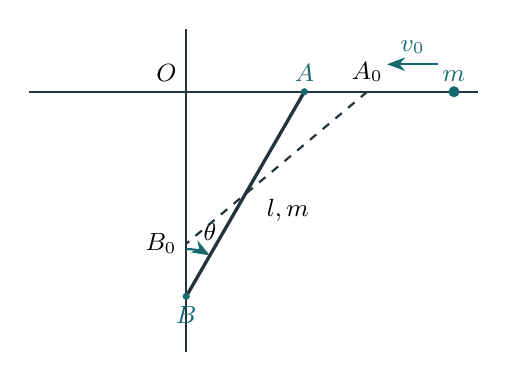
\begin{tikzpicture}[font=\small]
\draw[object](-2,0)--(3.7,0);\draw[object](0,.8)--(0,-3.3);
\draw[object,very thick](1.5,0)--(0,-2.598076211);
\fill[accent](1.5,0)circle(1.3pt)node[above]{$A$};
\fill[accent](0,-2.598076211)circle(1.3pt)node[below]{$B$};
\node[above left]at(0,0){$O$};\node[right]at(.9,-1.5){$l,m$};
\draw[motion](0,-1.998076211)arc(90:60:.6);\node at(.3,-1.78){$\theta$};

\draw[object,dashed](2.298133329,0)--(0,-1.928362829);
\node[above]at(2.298133329,0){$A_0$};\node[left]at(0,-1.928362829){$B_0$};
\fill[accent](3.4,0)circle(2pt)node[above]{$m$};\draw[motion](3.2,.35)--(2.55,.35)node[midway,above]{$v_0$};
\end{tikzpicture}\figcaption{图 7.18}\end{minipage}\end{center}

\Needspace{18\baselineskip}\subsection*{解答}

\begin{center}\begin{minipage}{\linewidth}\centering\begin{tikzpicture}[font=\small]
\draw[object](-2,0)--(3.7,0);\draw[object](0,.8)--(0,-3.3);
\draw[object,very thick](1.5,0)--(0,-2.598076211);
\fill[accent](1.5,0)circle(1.3pt)node[above]{$A$};
\fill[accent](0,-2.598076211)circle(1.3pt)node[below]{$B$};
\node[above left]at(0,0){$O$};\node[right]at(.9,-1.5){$l,m$};
\draw[motion](0,-1.998076211)arc(90:60:.6);\node at(.3,-1.78){$\theta$};

\fill[accent](.75,-1.299038106)circle(1pt)node[right]{$C$};
\draw[force](.75,-1.299038106)--(.75,-2.899038106)node[right]{$mg$};
\draw[force](1.5,0)--(1.5,1.3)node[right]{$N_A$};
\draw[force](0,-2.598076211)--(-.519615242,-2.598076211)node[left]{$N_B$};
\node at(.7,-3.9){受力示例：$\theta=30^\circ$，端点静止释放};
\end{tikzpicture}\figcaption{解图 7.18A\quad 杆的中点$C$是质心，重力从$C$向下；$A,B$分别沿两条直导轨运动。}\end{minipage}\end{center}
按解图7.18A，以导轨交点为原点，$x$ 向右、$y$ 向下。杆上端 $A=(l\sin\theta,0)$、下端 $B=(0,l\cos\theta)$，质心坐标为
\[x_C=\frac l2\sin\theta,\qquad y_C=\frac l2\cos\theta,\qquad
v_C^2=\frac{l^2}{4}\dot\theta^2.\]
质心惯量 $I_C=ml^2/12$，因此完整能量为
\[E=\frac12m v_C^2+\frac12I_C\dot\theta^2-mg\frac l2\cos\theta
=\frac{ml^2}{6}\dot\theta^2-\frac{mgl}{2}\cos\theta.\]
求导给 $\ddot\theta+(3g/2l)\sin\theta=0$，小角时
\[\boxed{T=2\pi\sqrt{\frac{2l}{3g}}.}\]
动力学另一解法保留约束力。令上端竖直支持为 $N_A$ 向上，下端水平力为 $N_B$ 向左记号：
\[m\ddot x_C=-N_B,\quad m\ddot y_C=mg-N_A,
\quad I_C\ddot\theta=\frac l2(N_B\cos\theta-N_A\sin\theta).\]
坐标二次求导为
\[\ddot x_C=\frac l2(\cos\theta\ddot\theta-\sin\theta\dot\theta^2),\quad
\ddot y_C=-\frac l2(\sin\theta\ddot\theta+\cos\theta\dot\theta^2).\]
代回转动式，$\dot\theta^2$ 项相消，得到 $(I_C+ml^2/4)\ddot\theta=-(mgl/2)\sin\theta$，与能量法一致。
\begin{center}\begin{minipage}{\linewidth}\centering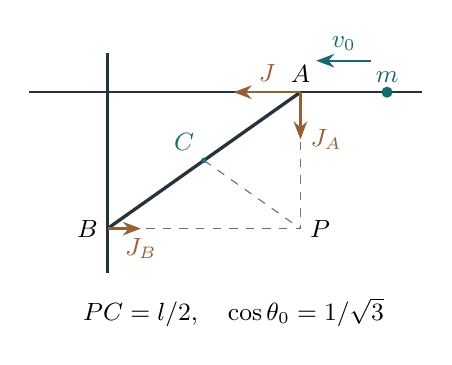
\begin{tikzpicture}[font=\small]
\draw[object](-1,0)--(4,0);\draw[object](0,.5)--(0,-2.3);
\coordinate(A)at(2.449489743,0);\coordinate(B)at(0,-1.732050808);\coordinate(P)at(2.449489743,-1.732050808);
\draw[object,very thick](A)--(B);\draw[guide](A)--(P)--(B);
\node[above]at(A){$A$};\node[left]at(B){$B$};\node[right]at(P){$P$};
\fill[accent](1.224744872,-.866025404)circle(1pt)node[above left]{$C$};\draw[guide](1.224744872,-.866025404)--(P);
\fill[accent](3.55,0)circle(2pt)node[above]{$m$};\draw[motion](3.35,.4)--(2.65,.4)node[midway,above]{$v_0$};
\draw[force](A)--(1.600961606,0)node[midway,above]{$J$};
\draw[force](A)--(2.449489743,-.600000000)node[right]{$J_A$};
\draw[force](B)--(.424264069,-1.732050808)node[below]{$J_B$};
\node at(1.6,-2.8){$PC=l/2,\quad \cos\theta_0=1/\sqrt3$};
\end{tikzpicture}\figcaption{解图 7.18B}\end{minipage}\end{center}
碰撞前杆在 $\theta_0$ 静止。解图7.18B的瞬心 $P=(l\sin\theta_0,l\cos\theta_0)$ 是两端速度垂线的交点，$PC=l/2$，杆关于它的惯量为
\[I_P=I_C+m(l/2)^2=ml^2/3.\]
碰撞瞬间两个导轨冲量关于 $P$ 均无矩，重力冲量矩可忽略。球碰后静止且不失能，因此
\[mv_0l\cos\theta_0=I_P|\omega_+|,\qquad
\frac12mv_0^2=\frac12I_P\omega_+^2.\]
消去 $\omega_+$，得 $I_P=ml^2\cos^2\theta_0$，所以右侧构型取 $\cos\theta_0=1/\sqrt3$。这也可看作杆端等效质量 $I_P/(l^2\cos^2\theta_0)$ 恰等于球质量，弹性碰撞才使球停下。
碰后杆回摆到左侧水平时质心升到导轨高度，所需势能为 $(mgl/2)\cos\theta_0$。再用能量：
\[\frac12mv_0^2=\frac{mgl}{2}\cos\theta_0,\qquad
\boxed{v_0=\sqrt{\frac{gl}{\sqrt3}}\simeq0.760\sqrt{gl}.}\]
瞬心随杆移动，可逐时用于计算动能；关于它的角动量导数还含下面的参考点速度项。
\subsubsection*{质心速度和两约束力的消元全步}
解图7.18A以向下的$y$为正，$A$沿水平轨、$B$沿竖直轨。
两端满足$OA=l\sin\theta,OB=l\cos\theta$，
质心是杆中点，因此
\[
\dot x_C=\frac l2\cos\theta\dot\theta,
\quad\dot y_C=-\frac l2\sin\theta\dot\theta,
\quad v_C^2=\frac{l^2}{4}(\cos^2\theta+\sin^2\theta)\dot\theta^2.
\]
水平、竖直动能与绕心动能相加，
\[
K=\frac{ml^2}{8}\dot\theta^2+\frac{ml^2}{24}\dot\theta^2
=\frac{ml^2}{6}\dot\theta^2.
\]
从端点角$\theta_m$静止释放的能量式还可写成
\[
\frac{ml^2}{6}\dot\theta^2=\frac{mgl}{2}(\cos\theta-\cos\theta_m),
\quad l\dot\theta^2=3g(\cos\theta-\cos\theta_m).
\]
求导得到完整角度方程，非转折段先约去$\dot\theta$，
转折点再由连续性恢复，小角才将$\sin\theta$换为$\theta$。

动力学法先由两平移式求两约束力。
将质心加速度分别代入两平移式，
\[
\begin{aligned}
N_A&=m\left[g+\frac l2(\sin\theta\ddot\theta+\cos\theta\dot\theta^2)\right],\\
N_B&=\frac{ml}{2}(\sin\theta\dot\theta^2-\cos\theta\ddot\theta).
\end{aligned}
\]
再代$C$点转矩，
\[
\begin{aligned}
I_C\ddot\theta
={}&\frac{ml^2}{4}\sin\theta\cos\theta\dot\theta^2
-\frac{ml^2}{4}\cos^2\theta\ddot\theta
-\frac{mgl}{2}\sin\theta\\
&-\frac{ml^2}{4}\sin^2\theta\ddot\theta
-\frac{ml^2}{4}\sin\theta\cos\theta\dot\theta^2\\
={}&-\frac{ml^2}{4}\ddot\theta-\frac{mgl}{2}\sin\theta.
\end{aligned}
\]
两个含$\dot\theta^2$的项恰好相消，
这一消元在有限角下也成立。
用$I_C=ml^2/12$合并惯性项，得到
$\ddot\theta+3g\sin\theta/(2l)=0$，与能量法完全一致。

\subsubsection*{瞬心的转动动能与移动参考点的力矩}
解图7.18B中的$P$是$A$竖线与$B$横线交点，
在每个构型都有$P=(l\sin\theta,l\cos\theta)$，
$C=P/2$，所以$PC=l/2$。
瞬时刚体速度可写成绕该位置的转动，
\[
I_P=I_C+mPC^2=ml^2/3,\qquad K=\frac12I_P\dot\theta^2.
\]
本题的$I_P$为常数，上式给出每个构型的动能。$P$随杆的位置移动，用各质点的地面速度定义关于$P$的角动量时，其导数为
\[
\frac{\dd\boldsymbol L_P}{\dd t}
=\boldsymbol\tau_P-\boldsymbol v_P\times(m\boldsymbol v_C).
\]
本题由于$\boldsymbol v_P=2\boldsymbol v_C$，叉积项恰为零；
因此关于$P$的角动量变化率等于所受合力矩。重力矩随构型改变，角动量随相应的力矩演化。

\subsubsection*{弹性碰撞中的两条守恒与构型匹配}
碰撞前杆已在右侧转折点静止，小球沿水平向左入射。
取碰撞瞬间的空间点$P$为取矩点，在极短时间内视几何构型不变。
上端导轨冲量沿$AP$、下端导轨冲量沿$BP$，都对$P$无矩；
重力的冲量矩相对碰撞冲量矩可忽略。
所以球杆系统关于这个点的碰撞前后角动量相等，
入射冲量臂为竖直距离$PA=l\cos\theta_0$。
记杆碰后角速度大小为$\omega_+$，两条关系为
\[
mv_0l\cos\theta_0=I_P\omega_+,\qquad
mv_0^2=I_P\omega_+^2.
\]
用第一式给$\omega_+=mv_0l\cos\theta_0/I_P$，代入第二式，
\[
mv_0^2=\frac{m^2v_0^2l^2\cos^2\theta_0}{I_P},
\quad I_P=ml^2\cos^2\theta_0.
\]
正入射速度可约去，代$I_P=ml^2/3$得
$\cos^2\theta_0=1/3$。
右侧杆仍在水平导轨以下，故取$0<\theta_0<\pi/2$、
$\cos\theta_0=1/\sqrt3$；另一符号不符合该构型。

杆端沿碰撞方向的速度为$v_A=l\cos\theta_0\omega_+$，
因此它的等效质量为$I_P/(l^2\cos^2\theta_0)$。
在该构型恰为$m$，弹性碰撞使小球停下并使$A$接过入射速度。
由两端速度关系得$|v_A|=v_0$、$|v_B|=\sqrt2v_0$及$\omega_+=\sqrt3v_0/l$。

\subsubsection*{约束冲量、碰后上升与模型条件}
水平总动量一般不守恒，因为竖直导轨对$B$可施加水平冲量。
题设等质量匹配构型中，杆碰后质心水平速度为$-v_0/2$，
而碰前球的水平动量为$-mv_0$，
故导轨给系统的水平冲量为$+mv_0/2$。
杆质心向下速度为$v_0/\sqrt2$，
所以上端导轨还给向下冲量$mv_0/\sqrt2$。
上端用双侧导轨承担这一向下冲量，下端由竖直导轨承担水平冲量。

题设为弹性碰撞，球的入射动能全部转为杆的动能。
碰撞后小球静止，杆的初动能为$mv_0^2/2$；
之后无摩擦摆动再单独使用杆的机械能守恒。
当杆摆到左侧水平，$y_C$从$l\cos\theta_0/2$降为0，
其实际高度上升$l\cos\theta_0/2$，因此
\[
\frac12mv_0^2=\frac12mgl\cos\theta_0,
\quad v_0^2=\frac{gl}{\sqrt3},\quad
v_0=3^{-1/4}\sqrt{gl}.
\]
击速由精确的$\cos\theta_0=1/\sqrt3$开方求得。
碰后从右侧出发的角速度使$\theta$减小，
杆先过竖直位置，再到左侧水平。
两个导轨约束力在各自端点的允许速度方向上均不做功，
但它们仍可改变系统动量，零功与零冲量要分开判断。


\Needspace{18\baselineskip}

\pdfbookmark[2]{第 19 题 两质量弹簧系统的相对振动}{q19}

\section*{第 19 题\quad 两质量弹簧系统的相对振动}

\tagline{M-07-19}

如图,在光滑水平面上,质量为\(m_{1}\)和\(m_{2}\)的两物体用劲度系数为\(k\)的弹簧相连.当弹簧为原长时,\(m_{1}\)与\(m_{2}\)相距\(l_{0}\),把弹簧压缩距离\(a\)后从静止释放.试求\(m_{1}\)和\(m_{2}\)的振动表达式.

\begin{center}\begin{minipage}{\linewidth}\centering\begin{tikzpicture}[font=\small,spring/.style={decorate,decoration={coil,aspect=.45,segment length=4pt,amplitude=3pt},thick}]
\draw[object,fill=white](-2.55,-.25)rectangle(-1.95,.25);\node at(-2.25,0){$m_1$};
\draw[object,fill=white](.45,-.25)rectangle(1.05,.25);\node at(.75,0){$m_2$};
\draw[spring](-1.95,0)--(.45,0);\node[above]at(-.75,.3){$k,l_0$};
\draw[guide](-3.5,-.3)--(1.6,-.3);\draw[guide](0,.25)--(0,.85);\node[above]at(0,.85){$C$};
\draw[<->](-2.25,-.65)--(.75,-.65)node[midway,below]{$l_0-a$};
\draw[axis](-3.5,-1.3)--(1.6,-1.3)node[right]{$x$};\node[below]at(0,-1.3){$0$};
\node at(-.6,-1.95){初始压缩状态，图示位置取$m_2=3m_1$};
\end{tikzpicture}\figcaption{图 7.19}\end{minipage}\end{center}

\Needspace{18\baselineskip}\subsection*{解答}

\begin{center}\begin{minipage}{\linewidth}\centering\begin{tikzpicture}[font=\small,spring/.style={decorate,decoration={coil,aspect=.45,segment length=4pt,amplitude=3pt},thick}]
\draw[object,dashed](-3.3,-.25)rectangle(-2.7,.25);\draw[object,dashed](.7,-.25)rectangle(1.3,.25);
\draw[object,fill=white](-2.925,-.25)rectangle(-2.325,.25);\node at(-2.625,0){$m_1$};
\draw[object,fill=white](.575,-.25)rectangle(1.175,.25);\node at(.875,0){$m_2$};
\draw[spring](-2.325,0)--(.575,0);\node[above]at(-1,.3){$k,l_0$};
\draw[guide](0,.25)--(0,.85);\node[above]at(0,.85){$C$};
\draw[motion](-2.625,-.65)--(-3.675,-.65)node[midway,below]{$\dot x_1$};
\draw[motion](.875,-.65)--(1.225,-.65)node[midway,below]{$\dot x_2$};
\draw[axis](-3.8,-1.4)--(1.7,-1.4)node[right]{$x$};\node[below]at(0,-1.4){$0$};
\node at(-1,-2.15){$q=-l_0/8,\quad\dot q>0,\quad m_2=3m_1$（位置与速度示意）};
\end{tikzpicture}\figcaption{解图 7.19A\quad 质心系中的速度分配；虚框为各自平衡位置，图示压缩后的回弹阶段。}\end{minipage}\end{center}
取两物体质心为原点，向右为正，$m_1$ 在左、$m_2$ 在右。水平外力为零且从静止释放，故
\[m_1x_1+m_2x_2=0.\]
令弹簧伸长量为 $q=x_2-x_1-l_0$，两物体的平移方程是
\[m_1\ddot x_1=kq,\qquad m_2\ddot x_2=-kq.\]
相减得到相对振动方程
\[\ddot q+k\left(\frac1{m_1}+\frac1{m_2}\right)q=0,\qquad
\mu=\frac{m_1m_2}{m_1+m_2},\quad\Omega=\sqrt{k/\mu}.\]
由压缩 $a$ 后静止释放，$q(0)=-a$、$\dot q(0)=0$，所以 $q=-a\cos\Omega t$。将 $x_2-x_1=l_0+q$ 与质心式联立：
\[\boxed{\begin{aligned}
x_1(t)&=-\frac{m_2}{m_1+m_2}(l_0-a\cos\Omega t),\\
x_2(t)&=\frac{m_1}{m_1+m_2}(l_0-a\cos\Omega t).
\end{aligned}}\]
解图7.19A的静态位置分别为 $x_{1e}=-m_2l_0/(m_1+m_2)$、$x_{2e}=m_1l_0/(m_1+m_2)$。位移 $X_1=x_1-x_{1e}$、$X_2=x_2-x_{2e}$ 分别是正、负的余弦，故
\[A_1=\frac{m_2a}{m_1+m_2},\quad A_2=\frac{m_1a}{m_1+m_2},
\quad A_1/A_2=m_2/m_1,\quad\phi_2-\phi_1=\pi.\]
分别解两端的方程时，也应保留平衡坐标。由质心关系得
\[
 x_2=-\frac{m_1}{m_2}x_1,\qquad
 q=-\frac{m_1+m_2}{m_2}x_1-l_0
   =-\frac{m_1+m_2}{m_2}X_1.
\]
于是 $m_1\ddot X_1=-k(m_1+m_2)X_1/m_2$。同理，
$q=(m_1+m_2)X_2/m_1$，故 $m_2\ddot X_2=-k(m_1+m_2)X_2/m_1$。
两式都含同一个约化质量 $\mu$。
\[
 X_1=C_1\cos\Omega t+D_1\sin\Omega t,\quad
 X_2=C_2\cos\Omega t+D_2\sin\Omega t.
\]
零初速度使 $D_1=D_2=0$；压缩初态给
$C_1=m_2a/(m_1+m_2)$、$C_2=-m_1a/(m_1+m_2)$，所以两端相位相反。
约化质量也可从动能的完整分解得到。设一般质心坐标为$X$，两球间距为$l_0+q$，则
\[x_1=X-\frac{m_2}{m_1+m_2}(l_0+q),
\qquad x_2=X+\frac{m_1}{m_1+m_2}(l_0+q).\]
代入$m_1\dot x_1^2/2+m_2\dot x_2^2/2$，交叉项相消，剩下
\[K=\frac12(m_1+m_2)\dot X^2+\frac12\mu\dot q^2.\]
图7.19A中两端反向运动只改变$q$，并未使$X$振动。求相对频率用$\mu$，求共同漂移则用总质量，两种“质量”对应不同运动变量。

相对位移法与逐球消元给出同一频率和幅相。总能量在质心系为 $E=\mu\dot q^2/2+kq^2/2=ka^2/2$。非零总初动量时，还须为两个坐标共同加上质心匀速漂移项。
\subsubsection*{分别求解两端的平衡偏置与相位}
令$M=m_1+m_2$，质心原点给$m_1x_1+m_2x_2=0$。
从初始间距$l_0-a$与这个条件联立，
\[
x_1(0)=-\frac{m_2}{M}(l_0-a),\qquad
x_2(0)=\frac{m_1}{M}(l_0-a).
\]
第一物体的牛顿式使用间距减自然长作为形变量，
\[
m_1\ddot x_1=k[(x_2-x_1)-l_0]
=-k\left(\frac{M}{m_2}x_1+l_0\right).
\]
乘$m_2/M$后，将平衡坐标从未知量中减去，
\[
\mu\ddot x_1=-k\left(x_1+\frac{m_2l_0}{M}\right),
\quad X_1=x_1+\frac{m_2l_0}{M},\quad
\ddot X_1+\Omega^2X_1=0.
\]
取正振幅$A_1$，$X_1=A_1\cos(\Omega t+\phi_1)$，
两个初值分别给
\[
A_1\cos\phi_1=\frac{m_2a}{M}>0,\qquad
-A_1\Omega\sin\phi_1=0.
\]
由正余弦符号一起确定$\phi_1=0\pmod{2\pi}$，
所以$A_1=m_2a/M$；正的初位移选定初相位为0。

对第二物体同样从它自己的受力式开始，
\[
m_2\ddot x_2=-k[(x_2-x_1)-l_0]
=-k\left(\frac{M}{m_1}x_2-l_0\right).
\]
乘$m_1/M$，令$X_2=x_2-m_1l_0/M$，得到
\[
\mu\ddot X_2=-kX_2,\quad
A_2\cos\phi_2=-\frac{m_1a}{M}<0,\quad
-A_2\Omega\sin\phi_2=0.
\]
故$\phi_2=\pi\pmod{2\pi}$、$A_2=m_1a/M$。
解图7.19A的虚框表示各自平衡位置，
初始压缩使左物体在自身平衡点右侧、右物体在自身平衡点左侧，
这正是两个初相位相差$\pi$的几何意义。
最后恢复绝对坐标，平衡间距仍为$l_0$，
两端振幅之和$A_1+A_2=a$才是弹簧的相对振幅。

\subsubsection*{动能交叉项、动量与能量分配}
一般地面初值下，质心坐标为$X$，速度为$V$，
相对伸长速度为$\dot q$。
两个绝对速度代入动能后逐项展开，
\[
\begin{aligned}
2K={}&m_1\left(V^2-2\frac{m_2}{M}V\dot q+\frac{m_2^2}{M^2}\dot q^2\right)\\
&+m_2\left(V^2+2\frac{m_1}{M}V\dot q+\frac{m_1^2}{M^2}\dot q^2\right)\\
={}&MV^2+\frac{m_1m_2(m_1+m_2)}{M^2}\dot q^2
=MV^2+\mu\dot q^2.
\end{aligned}
\]
两个交叉项相消，剩下的相对速度平方系数给约化质量。
总能量分成互不耦合的质心平动与内部振动，
\[
E=\frac12MV^2+\frac12\mu\dot q^2+\frac12kq^2.
\]
本题$V=0$，从压缩端静止释放得$E=ka^2/2$。
在质心系，$m_1\dot x_1=-m_2\dot x_2$，
两端动量等大反向，分别把同一个动量大小的平方除以各自两倍质量，得到动能比例，
\[
\frac{K_1}{K_2}=\frac{m_2}{m_1},\qquad
K_{1,\max}=\frac{m_2}{M}\frac{ka^2}{2},\quad
K_{2,\max}=\frac{m_1}{M}\frac{ka^2}{2}.
\]
较轻一端速度与动能更大，弹簧势能是系统共有的一项，在压缩端为$ka^2/2$。
若初始质心速度为$V_0$、相对初速度为$u$，
先取$X=X(0)+V_0t$、
$q=-a\cos\Omega t+(u/\Omega)\sin\Omega t$，
再按质量分数恢复两个地面坐标。
共同平移不改变内部频率，却会改变地面轨迹的极值时刻。

\subsubsection*{零频平移与无碰撞范围}
用两端相对平衡的位移写矩阵方程，特征式为
\[
\det\begin{pmatrix}k-m_1\omega^2&-k\\-k&k-m_2\omega^2\end{pmatrix}
=\omega^2[m_1m_2\omega^2-kM]=0.
\]
零根对应两端同位移的整体平移，
非零根$\Omega^2=kM/(m_1m_2)$对应$m_1X_1+m_2X_2=0$的内部模式。
质心用总质量描述匀速平移，相对坐标用约化质量描述有限频率的振动。
点质量模型要求压缩量$a<l_0$，使两端始终保持左右次序；
实际物体还须给彼此尺寸和弹簧压缩极限留出距离。
本题采用可拉压的线性弹簧，使压缩端和伸长端都遵循同一回复规律。


\Needspace{18\baselineskip}

\pdfbookmark[2]{第 20 题 缓慢缩短摆长时的振幅变化}{q20}

\section*{第 20 题\quad 缓慢缩短摆长时的振幅变化}

\tagline{M-07-20}

如图,单摆的原长为\(l_{0}\),在摆动过程中缓慢上拉,悬点位置不变而摆长逐渐缩短.试求当摆长缩短为原长之半,即\(l=\frac{l_{0}}{2}\)时的振幅与原振幅之比.

采用小角、缓慢变化的近似；分别说明角振幅与弧长振幅的变化。

\begin{center}\begin{minipage}{\linewidth}\centering\begin{tikzpicture}[font=\small]
\fill(0,0)circle(1.2pt)node[above]{$O$};\draw[object](0,0)--(1.026060430,-2.819077862);
\fill[accent](1.026060430,-2.819077862)circle(2pt);\draw[guide](0,0)--(0,-3.2);
\draw[guide](0,0)--(-1.026060430,-2.819077862);
\draw[motion](.7,-1.923234838)--(.35,-.961617419);\node[right]at(1.25,-1.1){缓慢上拉};
\draw[motion](0,-.75)arc(-90:-70:.75);\node at(.2,-1.0){$\theta$};
\node[right]at(.8,-2){$l$};
\end{tikzpicture}\figcaption{图 7.20\quad $l$为当前摆长，$\theta$为瞬时摆角；箭头表示缓慢上拉。}\end{minipage}\end{center}

\Needspace{18\baselineskip}\subsection*{解答}

\begin{center}\begin{minipage}{\linewidth}\centering\begin{tikzpicture}[font=\small]
\fill(0,0)circle(1.2pt)node[above]{$O$};\draw[object](0,0)--(1.026060430,-2.819077862);
\fill[accent](1.026060430,-2.819077862)circle(2pt);\draw[guide](0,0)--(0,-3.2);
\draw[guide](0,0)--(-1.026060430,-2.819077862);
\draw[motion](.7,-1.923234838)--(.35,-.961617419);\node[right]at(1.25,-1.1){缓慢上拉};
\draw[motion](0,-.75)arc(-90:-70:.75);\node at(.2,-1.0){$\theta$};
\node[right]at(.8,-2){$l$};
\node at(0,-3.9){$a(l)l^{3/4}=\mathrm{const}$};
\end{tikzpicture}\figcaption{解图 7.20A\quad $\theta$为瞬时摆角，$a$表示角振幅。}\end{minipage}\end{center}
用 $a(l)$ 表示角振幅，$P$ 表示振动周期，避免张力与周期都用 $T$。缓慢缩短要求 $|\dot l|/(l\Omega)\ll1$，且角振幅始终很小。每个局部周期内近似
\[\theta=a\cos(\Omega t+\phi),\quad\Omega=\sqrt{g/l},\quad
\langle\theta^2\rangle=a^2/2,\quad
\langle\dot\theta^2\rangle=a^2\Omega^2/2.\]
以悬点为重力势能零点，在局部定长近似中，角度转折处的能量为
\[E_{
\text{总}}=-mgl\cos a\simeq-mgl+\frac12mgla^2.\]
解图7.20A中径向张力满足局部准定长式 $F-mg\cos\theta=ml\dot\theta^2$，因此周期平均为
\[\langle F\rangle\simeq mg\left(1-\frac{a^2}{4}\right)
+ml\frac{a^2\Omega^2}{2}=mg(1+a^2/4).\]
\Needspace{17\baselineskip}$\dd l<0$ 时上拉力做正功 $-\langle F\rangle\dd l$。由功能关系，
\[-mg(1+a^2/4)\dd l
=\dd(-mgl+mgla^2/2)
=-mg\dd l+\frac12mga^2\dd l+mgla\dd a.\]
约去静态提升能量后，
\[\frac34a^2\dd l+la\dd a=0,
\quad\frac{\dd a}{a}=-\frac34\frac{\dd l}{l},
\quad a(l)l^{3/4}=a(l_0)l_0^{3/4}.\]
于是
\[\boxed{\frac{a(l_0/2)}{a(l_0)}=2^{3/4}\simeq1.682.}\]
这是角振幅的增加；线性弧长振幅 $A=la$ 的比值则为 $2^{-1/4}\simeq0.841$，两种振幅用各自的长度或角度单位表示。
从振幅关系可同时写出三种量随摆长的变化：
\[a\propto l^{-3/4},\qquad A=la\propto l^{1/4},
\qquad E_{\rm osc}=\frac12mgla^2\propto l^{-1/2}.\]
因此摆长减半时，角幅增大而弧长幅减小，振动能却增为$\sqrt2$倍。解图7.20A中小球的平均位置随绳收短而上升，拉力做功还包括静态势能增加$mg(l_0-l)$。平均张力的$mg$项贡献静态提升，$mga^2/4$项使振动能随收绳而增大。

用相椭圆的面积也可得到振幅关系。小角摆的振动能量 $E_{
\text{振}}=mgla^2/2$，慢变的作用量 $J=2\pi E_{
\text{振}}/\Omega\propto l^{3/2}a^2$ 保持，仍得 $al^{3/4}$ 恒定。慢变上拉使振动能随频率升高；给定变化较快的$l(t)$时，可直接按线性方程$\ddot\theta+2(\dot l/l)\dot\theta+(g/l)\theta=0$求瞬时摆角。
\subsubsection*{先从变摆长运动方程说明慢变的含义}
以$\theta$为角坐标，角动量为$p_\theta=ml^2\dot\theta$。
张力沿悬点连线，对悬点无矩，因此
\[
\frac{\dd}{\dd t}(ml^2\dot\theta)=-mgl\sin\theta,
\quad\ddot\theta+2\frac{\dot l}{l}\dot\theta+\frac gl\sin\theta=0.
\]
小角下将$\sin\theta$换为$\theta$，收绳引起的$2\dot l\dot\theta/l$保留。
该项在一个周期里较小，但在漫长的缩短过程中持续改变振幅。
局部频率$\Omega=\sqrt{g/l}$随长度变化，
相位应理解为$\int\Omega(t)\dd t+\phi_0$，
$\Omega t$只用于一个参数近似固定的短时间段。

缓慢且平滑的收绳满足
\[
\frac{|\dot l|}{l\Omega}\ll1,\qquad
\frac{|\ddot l|}{l\Omega^2}\ll1.
\]
起止时平滑改变收绳速度；缩短过程中的最大角幅也取远小于一弧度。

\subsubsection*{平方平均与功能关系的逐项计算}
在局部周期$P=2\pi/\Omega$内，$a,l$近似不变，
\[
\begin{aligned}
\langle\theta^2\rangle
&=\frac{a^2}{P}\int_0^P\cos^2(\Omega t+\phi)\dd t
=\frac{a^2}{2},\\
\langle\dot\theta^2\rangle
&=\frac{a^2\Omega^2}{P}\int_0^P\sin^2(\Omega t+\phi)\dd t
=\frac{a^2\Omega^2}{2}.
\end{aligned}
\]
平均张力中的重力投影为$mg(1-a^2/4)$，
向心项为$mla^2\Omega^2/2=mga^2/2$，
相加得到$mg(1+a^2/4)$，平方阶给振动部分的平均做功。
由于$\dd l<0$，张力方向向内，故它的功$-\langle F\rangle\dd l$为正。
用总能量微分，静态项$-mg\dd l$在两边相消后，
\[
-\frac14mga^2\dd l
=\frac12mga^2\dd l+mgla\dd a,
\quad\frac{\dd a}{a}=-\frac34\frac{\dd l}{l}.
\]
在$l_0$至$l$之间作定积分，
\[
\ln\frac{a(l)}{a(l_0)}=-\frac34\ln\frac l{l_0},
\quad\frac{a(l)}{a(l_0)}=(l/l_0)^{-3/4}.
\]
角振幅由上式给出，乘当前摆长$l$得到弧长振幅。

\subsubsection*{径向基线动能与径向加速度的功}
严格的径向方程和地面机械能为
\[
F=mg\cos\theta+ml\dot\theta^2-m\ddot l,
\quad E_{\text{地}}=\frac12m\dot l^2+\frac12ml^2\dot\theta^2-mgl\cos\theta.
\]
角度达到转折点时 $\dot\theta=0$，切向速度为零。若仍在收绳，摆球在这一刻沿径向以速度 $\dot l$ 向内移动。
将总能量分成基线
$E_b=m\dot l^2/2-mgl$与小角振动能$E_{\rm osc}$，
周期平均张力为$mg(1+a^2/4)-m\ddot l$。
由$\dot E_{\text{地}}=-F\dot l$并减去
$\dot E_b=m\dot l\ddot l-mg\dot l$，
径向加速度所做的功与径向基线动能变化恰好相消，剩下
\[
\langle\dot E_{\rm osc}\rangle=-\frac14mga^2\dot l.
\]
这与$E_{\rm osc}=mgla^2/2$的微分再次给出$3/4$指数。
局部定长的计算等效于先扣除径向基线。角度转折点的切向速度为零，径向速度仍是收绳速度。

\subsubsection*{相椭圆面积、角幅与弧长幅}
小角摆的共轭动量为$ml^2\dot\theta$，相椭圆面积
\[
J=\pi ml^2\Omega a^2=\pi m\sqrt g\,l^{3/2}a^2.
\]
参数缓变时$J$近似守恒，开平方仍得$al^{3/4}$恒定。
相平面取角度和角动量，惯量为$ml^2$。若改用弧长，质点的质量$m$进入相应的动能。

也可令弧长变量$s=l\theta$。
将线性角度方程完整变换后，
\[
\ddot s+\left(\frac gl-\frac{\ddot l}{l}\right)s=0.
\]
慢变时后项远小于$g/l$，局部谐振的弧长包络满足
$A\propto\Omega^{-1/2}\propto l^{1/4}$，
角幅$a=A/l$因而为$l^{-3/4}$。
从角度换成弧长时，保留角度方程中的一阶慢变项，弧长方程由此化为上式。先由局部频率求弧长幅，再除以摆长得到角幅。

\begin{center}\begin{minipage}{\linewidth}\centering
\begin{tikzpicture}[font=\small,x=7cm,y=4cm]
\draw[axis](.43,.72)--(1.13,.72)node[right]{$\lambda=l/l_0$};
\draw[axis](.43,.72)--(.43,1.82)node[above]{相对初值};
\draw[traj,domain=.5:1,samples=61]plot(\x,{\x^(-.75)});
\draw[object,domain=.5:1,samples=61]plot(\x,{\x^(-.5)});
\draw[guide,domain=.5:1,samples=61]plot(\x,{\x^(.25)});
\draw[guide](.5,.72)--(.5,1.681792831);\node[below]at(.5,.72){$1/2$};\node[below]at(1,.72){$1$};
\foreach \yy in {1,1.4,1.8}{\draw(.42,\yy)--(.44,\yy);\node[left]at(.42,\yy){$\yy$};}
\draw[traj](1.02,1.68)--(1.08,1.68)node[right]{角幅$a/a_0$};
\draw[object](1.02,1.42)--(1.08,1.42)node[right]{振动能$E_{\rm osc}/E_{{\rm osc},0}$};
\draw[guide](1.02,.9)--(1.08,.9)node[right]{弧长幅$A/A_0$};
\end{tikzpicture}
\figcaption{解图7.20B\quad 随摆长缓慢缩短，角幅、振动能与弧长幅分别按$\lambda^{-3/4},\lambda^{-1/2},\lambda^{1/4}$变化。}
\end{minipage}\end{center}
解图7.20B在$\lambda=1/2$给角幅$1.68179$、振动能$1.41421$、弧长幅$0.84090$。
拉绳总功还包括静态势能增加$mg(l_0-l)$；
若起止径向速度均为零，平均总功为这项提升能量加上振动能增量。
大角幅下，摆长缓变时仍可用作用量描述振幅演化，计算面积时取完整摆的非线性势能。


\Needspace{18\baselineskip}

\pdfbookmark[2]{第 21 题 小虫沿刚性摆杆爬行时的频率与振幅}{q21}

\section*{第 21 题\quad 小虫沿刚性摆杆爬行时的频率与振幅}

\tagline{M-07-21}

如图,质量为\(M\)、长为\(L\)的均匀刚性细杆的一端悬挂,可在铅垂面内绕悬点无摩擦地

摆动．质量为 \(m=\frac{M}{3}\) 的小虫相对杆以速度 \(v_{\mathrm{L}}\)
缓慢地沿杆向下爬行．开始时,杆静止并与竖直线夹 \(\theta_{0}\) 角(设
\(\theta_{0}\)
很小)；小虫位于杆上端的悬点．放开后,杆开始摆动,小虫开始爬行．

试求:1. 小虫沿杆爬行 \(l\) 距离时,杆摆动的圆频率.2.
小虫爬到杆下端时,杆摆动的幅度.

\begin{center}\begin{minipage}{\linewidth}\centering\begin{tikzpicture}[font=\small]
\fill(0,0)circle(1.2pt)node[above]{$O$};\draw[object,very thick](0,0)--(2,-3.464101615);
\fill[accent](1,-1.732050808)circle(2pt)node[right]{$m=M/3$};\draw[guide](0,0)--(0,-4.1);
\draw[<->](-.476313972,-.275)--(1.523686028,-3.739101615)node[midway,left]{$L,M$};
\draw[<->](.476313972,.275)--(1.476313972,-1.457050808)node[midway,right]{$s=l$};
\draw[motion](1.4,-2.2)--(1.7,-2.719615242)node[right]{$v_{\rm L}$};
\draw[motion](0,-.7)arc(-90:-60:.7);\node at(.3,-.9){$\theta$};
\end{tikzpicture}\figcaption{图 7.21}\end{minipage}\end{center}

\Needspace{18\baselineskip}\subsection*{解答}

\begin{center}\begin{minipage}{\linewidth}\centering\begin{tikzpicture}[font=\small]
\fill(0,0)circle(1.2pt)node[above]{$O$};\draw[object,very thick](0,0)--(2,-3.464101615);
\fill[accent](1,-1.732050808)circle(2pt)node[right]{$m=M/3$};\draw[guide](0,0)--(0,-4.1);
\draw[<->](-.476313972,-.275)--(1.523686028,-3.739101615)node[midway,left]{$L,M$};
\draw[<->](.476313972,.275)--(1.476313972,-1.457050808)node[midway,right]{$s=l$};
\draw[motion](1.4,-2.2)--(1.7,-2.719615242)node[right]{$v_{\rm L}$};
\draw[motion](0,-.7)arc(-90:-60:.7);\node at(.3,-.9){$\theta$};

\draw[force](1,-1.732050808)--(.350480947,-.607050808)node[left]{$f$};
\draw[force](1,-1.732050808)--(1,-3.232050808)node[below left]{$mg$};
\draw[force](1,-1.732050808)--(1.129903811,-1.657050808);
\draw[guide](1.129903811,-1.657050808)--(2,-1.2)node[right]{$Q$（切向约束）};
\node at(.7,-4.7){受力示例取$s=L/2$，角速度瞬时为零；摆角示意放大};
\end{tikzpicture}\figcaption{解图 7.21A}\end{minipage}\end{center}
用 $s$ 表示虫离悬点的距离，以 $\theta$ 为小摆角。杆、虫系统惯量与重力回复系数分别为
\[I(s)=\frac13ML^2+ms^2=\frac M3(L^2+s^2),\qquad
K(s)=g(ML/2+ms)=\frac{Mg}{6}(3L+2s).\]
关于悬点的角动量方程应写成
\[\frac{\dd}{\dd t}(I\dot\theta)=-K\sin\theta,
\quad I\ddot\theta+\dot I\dot\theta+K\theta\simeq0.\]
在一个局部周期内可将 $s$ 暂视不变，用它求瞬时频率：
\[\boxed{\Omega(s)=\sqrt{\frac{K(s)}{I(s)}}
=\sqrt{\frac{g(3L/2+s)}{L^2+s^2}}.}\]
振幅随整个爬行过程变化，需保留$\dot I\dot\theta$的累计作用。
解图7.21A中虫以小恒速向下爬，沿杆的摩擦向上。径向准平衡给 $f=mg\cos\theta+ms\dot\theta^2$。设局部振幅为 $a$、振动能量为 $E=Ia^2\Omega^2/2=Ka^2/2$，则
\[\langle\theta^2\rangle=E/K,\quad
\langle\dot\theta^2\rangle=E/I,\quad
\langle f\rangle=mg-\frac{mg}{2}\langle\theta^2\rangle
+ms\langle\dot\theta^2\rangle.\]
沿杆作用在系统中的机械功 $-\langle f\rangle\dd s$ 包括虫静态下降的 $-mg\dd s$；扣除此静态势能项后，振动能量变化为
\[\dd E=\left(\frac{mg}{2}\langle\theta^2\rangle
-ms\langle\dot\theta^2\rangle\right)\dd s.\]
代入 $m=M/3$、$I,K$，得
\[\frac{\dd E}{E}=\left[\frac1{3L+2s}-\frac{s}{L^2+s^2}\right]\dd s.\]
从 $0$ 积分到 $L$，
\[\ln\frac{E_L}{E_0}=\left[\frac12\ln(3L+2s)
-\frac12\ln(L^2+s^2)\right]_0^L
=\frac12\ln\frac56,\quad\frac{E_L}{E_0}=\sqrt{5/6}.\]
开始 $E_0=MgLa_0^2/4$，到端点时 $E_L=5MgLa_L^2/12$，因此
\[\boxed{\frac{a_L}{a_0}=\left(\frac3{10}\right)^{1/4}\simeq0.740.}\]
也可用慢变作用量 $E/\Omega$ 保持：$\Omega_L/\Omega_0=\sqrt{5/6}$，振幅 $a\propto(IK)^{-1/4}$，得到相同结果。这里把虫视为与杆共角速度、仅沿杆缓慢迁移的质点，沿杆作用与切向约束均计入相应方程，系统没有另加外力矩。
\subsubsection*{变惯量角动量与径向、切向作用的区分}
题中小虫爬行距离$l$在此记为$s$，即$s=l$，范围$0\le s\le L$。
解图7.21A的虫与杆具有共同的角速度，
虫相对杆的速度为沿杆的$v_{\rm L}$，地面速度还含切向分量$s\dot\theta$。
惯量与回复系数代入角动量方程，完整展开为
\[
\frac M3(L^2+s^2)\ddot\theta
+\frac{2M}{3}s\dot s\dot\theta
+\frac{Mg}{6}(3L+2s)\sin\theta=0.
\]
小角后，除以$M(L^2+s^2)/3$，
\[
\ddot\theta+\frac{2s\dot s}{L^2+s^2}\dot\theta
+\frac{g(3L/2+s)}{L^2+s^2}\theta=0.
\]
局部频率按当前$s$求出，振幅的演化由中间的缓变项给出。
可用$|\dot I|/(I\Omega)\ll1$和$|\dot K|/(K\Omega)\ll1$
表明局部周期内惯量与刚度的相对变化都很小，并使全过程角幅保持小。

解图7.21A将虫受杆的作用分为沿杆向上的$f$与切向的$Q$。
在杆系中，离心项沿杆，科里奥利和角加速度惯性项沿切向。
它们在径向式中的投影为零，切向和整体角动量方程仍须保留相应作用。
一般径向方程给
\[
f=mg\cos\theta+ms\dot\theta^2-m\ddot s.
\]
题设相对匀速爬行使$\ddot s=0$，才回到所用的$f$。
切向约束作用保证虫随杆摆动；对杆、虫系统列角动量时，
这些内部作用成对抵消，外力矩仍只有重力矩。

\subsubsection*{平均功与振动能微分的全步骤}
从局部谐振的动能、势能平均值分别等于$E/2$，
\[
\frac12I\langle\dot\theta^2\rangle=\frac E2,
\quad\frac12K\langle\theta^2\rangle=\frac E2,
\]
故$\langle\dot\theta^2\rangle=E/I$、$\langle\theta^2\rangle=E/K$。
用$\cos\theta\simeq1-\theta^2/2$平均沿杆作用，
\[
\langle f\rangle=mg-\frac{mgE}{2K}+\frac{msE}{I}.
\]
虫沿杆向下移动$\dd s>0$，相对滑移的机械功为$-\langle f\rangle\dd s$。
其中$-mg\dd s$同时改变静态重力势能；
扣除它后才是振动能的变化，
\[
\frac{\dd E}{E}=\left(\frac{mg}{2K}-\frac{ms}{I}\right)\dd s
=\left(\frac1{3L+2s}-\frac{s}{L^2+s^2}\right)\dd s.
\]
积分到任意位置$s$得
\[
\ln\frac{E(s)}{E(0)}
=\frac12\ln\frac{3L+2s}{3L}
-\frac12\ln\frac{L^2+s^2}{L^2}.
\]
因此
\[
\frac{E(s)}{E(0)}=
\sqrt{\frac{L(3L+2s)}{3(L^2+s^2)}}
=\frac{\Omega(s)}{\Omega(0)}.
\]
到$s=L$才取$\sqrt{5/6}$。
两端的回复系数分别为$MgL/2$、$5MgL/6$，
能量比等于角幅比的平方再乘刚度比：
\[
\frac{E_L}{E_0}=\frac{5MgLa_L^2/12}{MgLa_0^2/4}
=\frac53\frac{a_L^2}{a_0^2}.
\]
解出$a_L/a_0=(3/10)^{1/4}$。

\subsubsection*{直接对变参数振动能求导}
令$E_{\rm osc}=I\dot\theta^2/2+K\theta^2/2$。
由完整线性方程$I\ddot\theta+\dot I\dot\theta+K\theta=0$，
\[
\dot E_{\rm osc}
=-\frac12\dot I\dot\theta^2+\frac12\dot K\theta^2.
\]
用$\dot I=2ms\dot s$、$\dot K=mg\dot s$并作周期平均，
再次得到$\dot E/E=\dot K/(2K)-\dot I/(2I)$。
于是$E/\Omega$近似保持，而
\[
a(s)=a_0\left[\frac{I(0)K(0)}{I(s)K(s)}\right]^{1/4}.
\]
这条推导把缓变惯量的累计作用保留在能量导数中，
与平均沿杆作用的功逐项一致。

\subsubsection*{频率和振动能先升后降，角幅始终下降}
令$x=s/L$，局部频率和角幅可写成
\[
\frac{\Omega^2}{g/L}=\frac{3/2+x}{1+x^2},\qquad
\frac{a(s)}{a_0}=\left[\frac3{(1+x^2)(3+2x)}\right]^{1/4}.
\]
前一式对$x$求导，分子为
\[
1+x^2-2x(3/2+x)=1-3x-x^2.
\]
所以频率在$x_*=(\sqrt{13}-3)/2\simeq0.302776$达到最大，
$\Omega(x_*)/\Omega(0)\simeq1.04925$；
到杆端才下降到$\sqrt{5/6}\simeq0.91287$。
由于$E/\Omega$近似保持，振动能也先增后减。
而$I,K$均随$s$增加，它们的乘积单调增，故角幅一直减小。

\begin{center}\begin{minipage}{\linewidth}\centering
\begin{tikzpicture}[font=\small,x=6cm,y=8cm]
\draw[axis](0,.69)--(1.15,.69)node[right]{$x=s/L$};
\draw[axis](0,.69)--(0,1.13)node[above]{相对初值};
\draw[traj,domain=0:1,samples=101]plot(\x,{sqrt((3+2*\x)/(3*(1+\x^2)))});
\draw[object,domain=0:1,samples=101]plot(\x,{(3/((1+\x^2)*(3+2*\x)))^(.25)});
\fill[accent](.302775638,1.049249833)circle(1pt);\draw[guide](.302775638,.69)--(.302775638,1.049249833);
\node[above]at(.48,1.067){$\Omega/\Omega_0=E/E_0$};\node[right]at(.64,.80){$a/a_0$};
\foreach \yy in {.7,.8,.9,1,1.1}{\draw(-.01,\yy)--(.01,\yy);\node[left]at(-.01,\yy){$\yy$};}
\node[below]at(1,.69){$1$};\node[below]at(.302775638,.69){$x_*$};
\end{tikzpicture}
\figcaption{解图7.21B\quad 频率与振动能先升后降；角幅随虫离悬点的距离增加而单调下降。}
\end{minipage}\end{center}
解图7.21B的能量曲线指偏离竖直构型的振动能。小虫向杆端爬行时，沿杆作用对总机械能做负功。起步一段，竖直构型的重力势能下降得更快，两者之差进入图中的振动能，故振动能先上升。


\Needspace{18\baselineskip}

\pdfbookmark[2]{第 22 题 旋转圆盘支架上摆球的平衡与小振动}{q22}

\section*{第 22 题\quad 旋转圆盘支架上摆球的平衡与小振动}

\tagline{M-07-22}

如图7.22,圆盘在水平面内以匀角速\(\Omega\)绕竖直轴OO'旋转,盘上固连着两根同样高度的竖直支架.质量为\(m\)的小球与质量可忽略不计的\(T\)字形细杆相连,水平杆由支架支承,与小球相连的杆长为\(l\),悬点\(O'\)在转轴上,整个系统可在支架上无摩擦地摆动.

试求:1. 小球的平衡位置 .2. 小球作小幅摆动时的圆频率.

\begin{center}\begin{minipage}{\linewidth}\centering\begin{tikzpicture}[font=\small,x={(1cm,0cm)},y={(.6cm,.3cm)},z={(0cm,1cm)}]
\draw[object,variable=\u,domain=0:360,samples=101]plot({1.8*cos(\u)},{1.8*sin(\u)},0);
\draw[object](0,-1.5,0)--(0,-1.5,2.8);\draw[guide](0,0,-.35)--(0,0,3.4);
\draw[object,very thick](0,0,2.8)--(1.1,0,.894744112);\fill[accent](1.1,0,.894744112)circle(2pt)node[right]{$m$};
\draw[white,line width=3pt](0,1.5,0)--(0,1.5,2.8);\draw[object](0,1.5,0)--(0,1.5,2.8);
\draw[object,very thick](0,-1.5,2.8)--(0,1.5,2.8);
\fill(0,0,2.8)circle(1.2pt)node[above left]{$O'$};\node[below left]at(0,0,0){$O$};
\draw[motion,variable=\u,domain=0:30,samples=31]plot({.7*sin(\u)},0,{2.8-.7*cos(\u)});
\node[left]at(.22,0,1.85){$\theta$};\node[right]at(.65,0,1.65){$l$};
\draw[motion,variable=\u,domain=210:320,samples=31]plot({2*cos(\u)},{2*sin(\u)},0)node[right]{$\Omega$};
\end{tikzpicture}\figcaption{图 7.22}\end{minipage}\end{center}

\Needspace{18\baselineskip}\subsection*{解答}

\begin{center}\begin{minipage}{\linewidth}\centering\begin{tikzpicture}[font=\small]
\fill(0,0)circle(1.2pt)node[above]{$O'$};\draw[guide](0,0)--(0,-2.7);
\draw[object](0,0)--(2.165063509,-1.25);\fill[accent](2.165063509,-1.25)circle(2pt)node[above right]{$m$};
\draw[motion](0,-.65)arc(-90:-30:.65);\node at(.45,-.85){$\theta_*$};\node[above]at(1.2,-.7){$l$};
\draw[<->](0,-1.8)--(2.165063509,-1.8)node[midway,below]{$r=l\sin\theta_*$};
\draw[force](2.165063509,-1.25)--(2.165063509,-2.45)node[right]{$mg$};
\draw[force](2.165063509,-1.25)--(4.243524478,-1.25)node[right]{$m\Omega^2r$};
\draw[force](2.165063509,-1.25)--(.086602540,-.05)node[above left]{$T$};
\node at(1.8,-3.1){平衡示例：$\beta=2,\quad\theta_*=60^\circ$，相对速度为零};
\end{tikzpicture}\figcaption{解图 7.22A}\end{minipage}\end{center}
盘面参考系中，摆球相对转轴的有符号水平坐标为 $r=l\sin\theta$，离轴距离为 $|r|$。重力势能为 $-mgl\cos\theta$。离心力的水平分量为 $m\Omega^2r$，从轴到 $r$ 的功为
\[W_{
\rm cf}=\int_0^r m\Omega^2R\dd R=\frac12m\Omega^2r^2,\]
故离心势能为其负值。杆力不做相对功，科里奥利力垂直摆动速度，有效势能为
\[U(\theta)=-mgl\cos\theta-\frac12m\Omega^2l^2\sin^2\theta.\]
驻值条件与曲率为
\[U'=ml^2\sin\theta(g/l-\Omega^2\cos\theta)=0,\]
\[U''=ml^2[(g/l)\cos\theta-\Omega^2\cos^2\theta+\Omega^2\sin^2\theta].\]
因此有以下分支：$\theta=0$ 始终是平衡；$\theta=\pi$ 也是平衡但 $U''=-ml^2(g/l+\Omega^2)<0$，始终不稳。倾斜分支只在 $\Omega^2\ge g/l$ 时存在，满足
\[\cos\theta_*=\frac{g}{l\Omega^2},\qquad
\theta=\pm\theta_*\pmod{2\pi}.\]
解图7.22A中的有符号摆角允许两侧镜像构型。对低于临界的转速，$U''(0)>0$，零角稳定；高于临界，零角不稳，倾斜分支的曲率
\[U''(\theta_*)=ml^2\Omega^2\sin^2\theta_*>0\]
给两个稳定位置。
\begin{center}\begin{minipage}{\linewidth}\centering\begin{tikzpicture}[font=\small,x=2cm,y=1.8cm]
\draw[axis](-2.4,0)--(2.5,0)node[right]{$\theta$};
\draw[axis](0,-.5)--(0,1.65)node[above]{$[U-U(0)]/(mgl)$};
\draw[object,domain=-2.2:2.2,samples=121]plot(\x,{1-cos(deg(\x))-.2*sin(deg(\x))^2});
\draw[guide,domain=-2.2:2.2,samples=121]plot(\x,{1-cos(deg(\x))-.5*sin(deg(\x))^2});
\draw[traj,domain=-2.2:2.2,samples=121]plot(\x,{1-cos(deg(\x))-1.1*sin(deg(\x))^2});
\node at(-1.6,1.85){黑实线$\beta=.4$};\node at(1.6,1.85){蓝实线$\beta=2.2$};\node at(0,2.25){虚线$\beta=1$};
\end{tikzpicture}\figcaption{解图 7.22B}\end{minipage}\end{center}
解图7.22B中的势阱曲率决定稳定点附近的回复强弱。运动方程是 $ml^2\ddot\theta=-U'(\theta)$。在稳定点 $\theta_e$ 附近令 $\theta=\theta_e+\delta$，驻值常数项为零，一阶方程为
\[\ddot\delta+\frac{U''(\theta_e)}{ml^2}\delta=0.\]
所以两个转速区域的小振动圆频率分别为
\[\boxed{\omega_{
\text{低}}=\sqrt{g/l-\Omega^2},\qquad
\omega_{
\text{倾斜}}=\Omega|\sin\theta_*|
=\Omega\sqrt{1-\frac{g^2}{l^2\Omega^4}}.}\]
临界 $\Omega^2=g/l$ 时，二阶曲率为零。对非零小角，
\[U(\theta)-U(0)=\frac12mgl(1-\cos\theta)^2
=\frac18mgl\theta^4+O(\theta^6)>0.\]
零角是非线性稳定极小，线性频率为零。临界处的实际小幅运动由四次势能决定，周期见下面的能量积分。
\subsubsection*{支架约束、离心功与广义惯量}
图7.22的水平横杆是摆动的铰轴，球的相对轨迹位于随圆盘转动的竖直平面。
在该平面取水平$\hat{\boldsymbol x}$、竖直向上$\hat{\boldsymbol z}$，
悬杆位置相对$O'$为$l\sin\theta\hat{\boldsymbol x}-l\cos\theta\hat{\boldsymbol z}$。
相对速度为
\[
\boldsymbol v_{\rm rel}=l\dot\theta
(\cos\theta\hat{\boldsymbol x}+\sin\theta\hat{\boldsymbol z}).
\]
因圆盘角速度沿$\hat{\boldsymbol z}$，科里奥利力为
$-2m\Omega l\dot\theta\cos\theta\hat{\boldsymbol y}$，
垂直摆动平面，由支架约束承担，对$\theta$的广义力为零。
横铰杆限制了方位自由度，所以这里按一个摆角求运动。

离心力的切向投影为$m\Omega^2r\cos\theta$，
从$\theta$到$\theta+\dd\theta$的功为
\[
\dd W=m\Omega^2r\cos\theta\,l\dd\theta
=m\Omega^2r\dd r.
\]
从转轴积分至$r=l\sin\theta$，得$W=m\Omega^2r^2/2$，
故有效势的这一项为 $-m\Omega^2r^2/2$。
角动能为 $ml^2\dot\theta^2/2$，所以势阱曲率除以广义惯量 $ml^2$ 得角频率平方。

\subsubsection*{平衡分支逐项代入与存在条件}
定义无量纲转速$\beta=\Omega^2l/g\ge0$，
\[
\frac{U-U(0)}{mgl}=1-\cos\theta-\frac\beta2\sin^2\theta,
\quad U'=mgl\sin\theta(1-\beta\cos\theta).
\]
驻值有两种因子为零：$\sin\theta=0$给$0,\pi\pmod{2\pi}$，
另一因子给$\cos\theta=1/\beta$。
在实角范围 $\beta\ge1$ 取 $\theta=\pm\arccos(1/\beta)$。同时保留由 $\sin\theta=0$ 得到的两条竖直分支。

在$\theta=0$代入曲率，得$U''=mgl(1-\beta)$，
所以$\beta<1$稳定、$\beta>1$不稳。
在倒置位置$\theta=\pi$代入，
$U''=-mgl(1+\beta)<0$，任何转速下均不稳。
在倾斜点代$g/l=\Omega^2\cos\theta_*$，
\[
\frac{U''(\theta_*)}{ml^2}
=\Omega^2\cos^2\theta_*
-\Omega^2\cos^2\theta_*+\Omega^2\sin^2\theta_*
=\Omega^2\sin^2\theta_*>0.
\]
该曲率在 $\beta>1$ 时严格为正，$\beta=1$ 时倾斜分支与零角合并，稳定性由四次项确定。

\subsubsection*{倾斜点的一阶展开与局部幅度限制}
令$S=\sin\theta_*,C=\cos\theta_*$，写$\theta=\theta_*+\delta$。
一阶展开为$\sin\theta=S+C\delta$、$\cos\theta=C-S\delta$，
则回复函数
\[
\begin{aligned}
\left(\frac gl-\Omega^2\cos\theta\right)\sin\theta
={}&\left(\frac gl-\Omega^2 C\right)S\\
&+\left[\left(\frac gl-\Omega^2 C\right)C+\Omega^2S^2\right]\delta
+O(\delta^2).
\end{aligned}
\]
平衡条件使第一项及方括号中的前项相消，
剩下$\ddot\delta+\Omega^2S^2\delta=0$，
与势能曲率法一致。两个镜像位置的$S$符号相反，
回复系数均为 $\Omega^2 S^2$，圆频率同为 $\Omega|S|$。

在临界附近令$\beta=1+\varepsilon$、$0<\varepsilon\ll1$。
由$\cos\theta_*=1/(1+\varepsilon)$得
\[
\theta_*\simeq\sqrt{2\varepsilon},\qquad
\omega_{\text{倾斜}}\simeq\sqrt{2g\varepsilon/l}.
\]
在临界附近，将局部角幅取为 $A\ll|\theta_*|$，运动留在同一势阱的近底部。
势垒高度可直接算为
\[
U(0)-U(\theta_*)=\frac{mgl}{2\beta}(\beta-1)^2.
\]
势垒随 $(\beta-1)^2$ 降低，单阱内运动的能量范围也随之缩小。
从临界下侧逼近时，幅值平方与 $1-\beta$ 同阶便会使四次项与二次项同阶。

\begin{center}\begin{minipage}{\linewidth}\centering
\begin{tikzpicture}[font=\small,x=2cm,y=1.3cm]
\draw[axis](0,-1.5)--(3.2,-1.5)node[right]{$\beta=\Omega^2l/g$};
\draw[axis](0,-1.5)--(0,1.55)node[above]{$\theta_e$};
\draw[traj](0,0)--(1,0);\draw[guide](1,0)--(3,0);
\draw[traj,domain=1:3,samples=101]plot(\x,{rad(acos(1/\x))});
\draw[traj,domain=1:3,samples=101]plot(\x,{-rad(acos(1/\x))});
\fill(1,0)circle(1.2pt);\draw[guide](1,-1.5)--(1,-.1);
\node[below]at(1,-1.5){$1$};\node[left]at(0,0){$0$};
\node[right]at(2.6,1.18){稳定};\node[right]at(2.6,-1.18){稳定};\node[above]at(2.2,0){不稳定};
\end{tikzpicture}
\figcaption{解图7.22C\quad 下垂附近的平衡分支。实线为稳定支，零角的虚线支不稳定；临界点仍非线性稳定。}
\end{minipage}\end{center}
解图7.22C中，$\beta=1$处的零角平衡由高阶势能项维持稳定。
此时有效势相对零角的精确增量为
$mgl(1-\cos\theta)^2/2$，对非零小角严格为正，
零角仍是稳定极小，回复力矩的首项为三次项。

\subsubsection*{临界点的非线性周期}
临界势能首项为$mgl\theta^4/8$，
运动方程首项为$\ddot\theta+g\theta^3/(2l)=0$。
若小角幅为$A$，从端点静止释放，能量给
\[
\dot\theta^2\simeq\frac{g}{4l}(A^4-\theta^4).
\]
用$u=\theta/A$换元，四分之一周期再乘四，
\[
T(A)\simeq\frac8A\sqrt{\frac lg}
\int_0^1\frac{\dd u}{\sqrt{1-u^4}}.
\]
积分为有限的纯数，故$T\propto A^{-1}$。
每个非零小角幅对应周期运动。幅值趋零时，周期按 $A^{-1}$ 发散，对应于临界点的零线性频率。


\Needspace{18\baselineskip}

\pdfbookmark[2]{第 23 题 弹性碰撞激发弹簧连接双质点振动}{q23}

\section*{第 23 题\quad 弹性碰撞激发弹簧连接双质点振动}

\tagline{M-07-23}

如图,在光滑水平面上有三质点A、B、C,质量分别为\(m_{1}\)、\(m_{2}\)和\(m_{3}\),三质点位于同一直线上,开始时B和C静止,用劲度系数为k的弹簧(质量忽略)相连.开始时弹簧无形变。质点A以初速\(v_{0}\)沿连线方向与B作完全弹性碰撞.

以 \(A\) 和 \(B\) 的碰撞点为坐标原点, 连线为 \(x\) 轴, 试求碰后质点
\(B\) 的运动规律. 2. 设 \(m_{2}=m_{3}=m\), 为使质点 \(A\) 和 \(B\)
在碰后重新相遇, 但不相碰(即相遇时速度相同), 试问比值 \(\frac{m_{1}}{m}\)
应为多少?

\begin{center}\begin{minipage}{\linewidth}\centering\begin{tikzpicture}[line cap=round,line join=round,spring/.style={decorate,decoration={coil,aspect=.45,segment length=4pt,amplitude=3pt},thick}]\fill[accent] (-1.7,0) circle (.17);\node[above] at (-1.7,.2) {$A,m_1$};\draw[motion] (-1.4,0)--(-.65,0) node[above] {$v_0$};\draw[object,fill=white] (-0.3,-.3) rectangle (0.3,.3);\node at (0,0) {$m_2$};\draw[object,fill=white] (1.7,-.3) rectangle (2.3,.3);\node at (2,0) {$m_3$};\draw[spring] (0.30000000000000004,0)--(1.7,0);\draw[guide] (-.6,-.4)--(2.6,-.4);\node[above] at (0,.35) {$B$};\node[above] at (2,.35) {$C$};\node[above] at (1,.1) {$k,l_0$};\end{tikzpicture}\figcaption{图 7.23}\end{minipage}\end{center}

\Needspace{18\baselineskip}\subsection*{解答}

\begin{center}\begin{minipage}{\linewidth}\centering\begin{tikzpicture}[font=\small,spring/.style={decorate,decoration={coil,aspect=.45,segment length=4pt,amplitude=3pt},thick}]
\fill[accent] (-1.7,0) circle (.17);\node[above] at (-1.7,.2) {$A,m_1$};\draw[motion] (-1.4,0)--(-.65,0) node[above] {$v_0$};\draw[object,fill=white] (-0.3,-.3) rectangle (0.3,.3);\node at (0,0) {$m_2$};\draw[object,fill=white] (1.7,-.3) rectangle (2.3,.3);\node at (2,0) {$m_3$};\draw[spring] (0.30000000000000004,0)--(1.7,0);\draw[guide] (-.6,-.4)--(2.6,-.4);\node[above] at (0,.35) {$B$};\node[above] at (2,.35) {$C$};\node[above] at (1,.1) {$k,l_0$};
\node at(.3,1.15){碰前构型};
\begin{scope}[yshift=-2.4cm]
\node at(-1.7,.2){$A$};\node at(0,.2){$B$};\node at(2,.2){$C$};
\draw[motion](-1.7,-.35)--(-1.121237043,-.35)node[midway,below]{$v_A$};
\draw[motion](0,-.35)--(1.478762957,-.35)node[midway,below]{$v_B$};

\node at(2,-.35){$0$};\node at(.3,-1.1){碰后速度示例：$m_2=m_3=m,\ m_1/m=r_*$};
\end{scope}
\end{tikzpicture}\figcaption{解图 7.23A\quad 上行给出碰前的位置，下行的箭头给出碰后速度。}\end{minipage}\end{center}
解图7.23A把第一次碰撞与随后两物体的质心运动分开；解图7.23B中的间隙曲线用于判断以后是否再次接触。

碰撞远短于弹簧振动时间，弹簧来不及传递有限冲量。以第一次碰撞后为 $t=0$，一维弹性碰撞的动量和能量关系给
\[v_A=\frac{m_1-m_2}{m_1+m_2}v_0,\qquad
v_B=\frac{2m_1}{m_1+m_2}v_0,\quad v_C=0.\]
求碰后速度的中间步骤是
\[
 m_1v_0=m_1v_A+m_2v_B,\qquad
 m_1v_0^2=m_1v_A^2+m_2v_B^2.
\]
将第二式整理为 $m_1(v_0-v_A)(v_0+v_A)=m_2v_B^2$，
再用第一式的 $m_1(v_0-v_A)=m_2v_B$，非零碰撞支给
$v_0+v_A=v_B$。与动量式联立，便得到前面的两个速度。
弹簧在碰撞前为原长，碰撞极短，$C$ 的速度仍为零。

此后 $B,C$ 的质心匀速运动，速度及初始位置为
\[V=\frac{m_2v_B}{m_2+m_3},\qquad
X(0)=\frac{m_3l_0}{m_2+m_3},\quad X(t)=X(0)+Vt.\]
取弹簧伸长 $q=x_C-x_B-l_0$，相减两质点运动式得
\[\ddot q+\Omega^2q=0,\qquad
\Omega^2=k\left(\frac1{m_2}+\frac1{m_3}\right).\]
初值为 $q(0)=0,\dot q(0)=-v_B$，故 $q=-(v_B/\Omega)\sin\Omega t$。再由质心位置和间距消元，
\[\boxed{x_B(t)=Vt+\frac{m_3}{m_2+m_3}\frac{v_B}{\Omega}\sin\Omega t.}\]
常量 $X(0)$ 正好抵消 $B$ 在质心系中的静态负坐标。在质心系中令 $X_B'=x_B'-x_B'(0)$，则
\[x_B'(0)=-\frac{m_3l_0}{m_2+m_3},\quad
\dot X_B'(0)=v_B-V=\frac{m_3v_B}{m_2+m_3},\quad
\ddot X_B'+\Omega^2X_B'=0.\]
由此仍得上述正弦项，再加质心漂移就是实验室位置。$A$ 则有 $x_A=v_At$。
\begin{center}\begin{minipage}{\linewidth}\centering\begin{tikzpicture}[font=\small,x=1cm,y=1cm]
\draw[axis](0,0)--(6.8,0)node[right]{$u=\Omega t$};
\draw[axis](0,-.7)--(0,3)node[above]{$g(u)/3$};
\draw[traj,domain=0:6.5,samples=181]plot(\x,{(\x+4.603338849*sin(deg(\x)))/3});
\fill[accent](4.493409458,0)circle(1.2pt);\node[below]at(4.493409458,-.3){$u_*$};
\draw[guide](3.141592654,0)--(3.141592654,2.4);\node[below]at(3.141592654,-.1){$\pi$};
\node[below]at(6.283185307,-.1){$2\pi$};\node at(3,2.8){$g(u)=u+r_*\sin u\ge0$};
\end{tikzpicture}\figcaption{解图 7.23B}\end{minipage}\end{center}
当 $m_2=m_3=m$，令 $r=m_1/m$、$u=\Omega t$、$\Omega=\sqrt{2k/m}$。两轨迹为
\[x_B=\frac{rv_0}{r+1}\left(t+\frac{\sin u}{\Omega}\right),
\qquad x_A=\frac{(r-1)v_0}{r+1}t.\]
再次接触但没有相对碰撞速度，需同时满足 $x_B=x_A$、$\dot x_B=\dot x_A$，即
\[u+r\sin u=0,\qquad 1+r\cos u=0.\]
因此 $\sin u=-u/r$、$\cos u=-1/r$，两者均负，最早相切在第三象限。相除及平方相加分别给
\[\tan u=u,\qquad r=\sqrt{1+u^2}.\]
对 $(\pi,3\pi/2)$ 内的根迭代，得
\[u_*=4.493409458,\qquad
\boxed{m_1/m=4.603338849,\quad t_*=u_*/\Omega.}\]
图中间隙 $x_B-x_A\propto u+r\sin u$ 在 $t_*$ 之前始终非负、在这里触零后再增大。后续负波瓣的切触候选对应更大的 $r$。此时首个负波瓣已出现有限相对速度的接触，之后从该次碰撞所得的速度继续计算。
\subsubsection*{初碰、质心系初值与两种动量}
第一次碰撞很短，弹簧力在这段时间内没有有限冲量，
所以只对$A,B$联立动量及弹性能量式。
$C$没有受到碰撞冲量，速度仍为零。
解图7.23A的上行对应碰前构型，下行单列各物体的碰后速度。碰撞点为 $A,B$ 在 $t=0$ 的共同位置。
记 $B,C$ 的总质量为 $N=m_2+m_3$，其质心位置和速度分别为 $X_G,V_G$。
\[
X_G(0)=\frac{m_3l_0}{N},\quad
V_G=\frac{m_2v_B}{N}
=\frac{2m_1m_2v_0}{(m_1+m_2)N}.
\]
两点在质心系的初始坐标与速度分别为
\[
\begin{aligned}
x_B'(0)&=-m_3l_0/N,&v_B'(0)&=v_B-V_G=m_3v_B/N,\\
x_C'(0)&=m_2l_0/N,&v_C'(0)&=-V_G=-m_2v_B/N.
\end{aligned}
\]
两质点在质心系中的动量等大反向，地面系的总动量则为 $NV_G=m_2v_B$。

\subsubsection*{质心系牛顿方程、正振幅和初相位}
用$U_B=x_B'-x_B'(0)$、$U_C=x_C'-x_C'(0)$表示各自偏离平衡的量。
质心条件给$m_2U_B+m_3U_C=0$，
弹簧伸长为$q=U_C-U_B$，故
\[
q=-\frac{m_2+m_3}{m_3}U_B,
\quad m_2\ddot U_B=kq=-\frac{kN}{m_3}U_B.
\]
约化质量与角频率分别为
\[
\mu=\frac{m_2m_3}{N},\qquad
\Omega=\sqrt{k/\mu}=\sqrt{\frac{kN}{m_2m_3}}.
\]
取$U_B=A_B\cos(\Omega t+\phi_B)$、$A_B>0$，
两个初值给
\[
A_B\cos\phi_B=0,\qquad
-A_B\Omega\sin\phi_B=\frac{m_3v_B}{N}>0.
\]
所以$\phi_B=-\pi/2\pmod{2\pi}$，
$A_B=m_3v_B/(N\Omega)$。
先得到完整质心系位置
\[
x_B'(t)=-\frac{m_3l_0}{N}
+\frac{m_3v_B}{N\Omega}\sin\Omega t,
\]
再加回$X_G(0)+V_Gt$，两个静态常数相消，
\[
\begin{aligned}
x_B(t)&=V_Gt+\frac{m_3v_B}{N\Omega}\sin\Omega t\\
&=\frac{2m_1v_0}{(m_1+m_2)(m_2+m_3)}
\left[m_2t+\frac{m_3}{\Omega}\sin\Omega t\right].
\end{aligned}
\]
这给出全部质量和刚度参数；
$x_A=(m_1-m_2)v_0t/(m_1+m_2)$则为自由来球的直线。
在 $t=0$ 正弦位移和漂移位移都为零。对正弦项求导并与漂移速度相加，得 $\dot x_B(0)=m_3v_B/N+V_G=v_B$。

\subsubsection*{弹簧振幅、内部能量与轨迹的适用段}
由$q(0)=0,\dot q(0)=-v_B$，
\[
q=-\frac{v_B}{\Omega}\sin\Omega t,
\qquad E_{\text{内}}=\frac12\mu v_B^2.
\]
$B,C$在碰后的总动能还包含质心平动，
\[
\frac12m_2v_B^2=\frac12NV_G^2+\frac12\mu v_B^2.
\]
上式右端依次为质心平动能与内部振动能。自由振动段取 $v_B/\Omega<l_0$ 以保持 $B,C$ 的左右次序。若考虑弹簧压并或物体尺寸，将允许压缩量代入 $q(t)$ 求自由轨迹的终点。

\subsubsection*{接触的双根与初始分离}
当$m_2=m_3=m$，定义$r=m_1/m$、$u=\Omega t$。
实际间隙可写为
\[
G(t)=x_B-x_A=\frac{v_0}{(r+1)\Omega}g(u),
\quad g(u)=u+r\sin u.
\]
其初始导数为$\dot G(0)=v_0>0$，
表示第一次弹性碰撞后两点立即分开，再次相遇考察 $u>0$。
切触要求$g=0,g'=0$，所以
\[
\sin u_*=-u_*/r,\qquad\cos u_*=-1/r.
\]
由平方相加得$r^2=1+u_*^2$，
因$u_*>0$、$r>0$，正弦余弦同负，首个允许区间是第三象限。
两式相除得到 $\tan u_*=u_*$，并以两式的符号选取第三象限。
对$F(u)=\tan u-u$，在$(\pi,3\pi/2)$有$F'=\tan^2u>0$，
且两端函数异号，因此根唯一。
例如从$u_0=4.5$作牛顿迭代，
\[
u_{n+1}=u_n-\frac{\tan u_n-u_n}{\tan^2u_n},
\]
给出$u_*=4.493409458\cdots$、$r_*=4.603338849\cdots$。
时间也可直接用质量写成
\[
t_*^2=\frac{r_*^2-1}{\Omega^2}
=\frac{m_1^2-m^2}{2km},\qquad m_1>m.
\]

\subsubsection*{切触前后的间隙}
在$0<u\le\pi$，$g(u)>0$。
首个负正弦波瓣$(\pi,2\pi)$内，$g\ge0$等价于
\[
r\le h(u)=-\frac u{\sin u}.
\]
这个函数在两端趋于正无穷，导数的分子为
$Q(u)=-\sin u+u\cos u$，且$Q'=-u\sin u>0$。
由于$Q(\pi)=-\pi<0$、$Q(3\pi/2)=1>0$，
它只有一个零点，正是$u_*$，所以$h$的唯一最小值就是$r_*$。
临界质量比下，首负波瓣内只有这里触零，其他时刻间隙均正。
在 $u=2\pi$ 处直接得 $g(2\pi)=2\pi$。此后对 $u>2\pi$，有
\[
g(u)\ge u-r_*>2\pi-r_*>0.
\]
于是从首次分离到任意以后时刻，临界自由轨迹均不穿过零线。
切点的二阶导数$g''(u_*)=-r_*\sin u_*=u_*>0$，
切触瞬间两点速度相等，$g''(u_*)>0$ 使 $B$ 随即相对 $A$ 加速离开，二者的速度沿自由解连续接续。

若$r<r_*$，两点不再次接触；
若$r>r_*$，首个负波瓣内已有间隙过零，并以非零相对速度碰撞。
较晚第三象限的根所需的 $r$ 更大。这个范围先发生有限速的再碰，随后用新的速度重建轨迹。解图7.23B恰处于有无有限速再碰的临界。


\Needspace{18\baselineskip}

\pdfbookmark[2]{第 24 题 三球双弹簧系统的特征频率和振型}{q24}

\section*{第 24 题\quad 三球双弹簧系统的特征频率和振型}

\tagline{M-07-24}

如图7.24,质量为\(M\)的小球两侧分别用劲度系数均为\(k\)的弹簧与两个质量均为\(m\)的小球连成一直线,水平放置,忽略一切阻力和摩擦力.试求特征频率和振动模式.

\begin{center}\begin{minipage}{\linewidth}\centering\begin{tikzpicture}[line cap=round,line join=round,spring/.style={decorate,decoration={coil,aspect=.45,segment length=4pt,amplitude=3pt},thick}]\draw[object,fill=white] (-0.3,-.3) rectangle (0.3,.3);\node at (0,0) {$m$};\draw[object,fill=white] (1.7,-.3) rectangle (2.3,.3);\node at (2,0) {$M$};\draw[spring] (0.30000000000000004,0)--(1.7,0);\draw[object,fill=white] (3.7,-.3) rectangle (4.3,.3);\node at (4,0) {$m$};\draw[spring] (2.3,0)--(3.7,0);\draw[guide] (-.6,-.4)--(4.6,-.4);\node[above] at (1,.15) {$k$};\node[above] at (3,.15) {$k$};\end{tikzpicture}\figcaption{图 7.24}\end{minipage}\end{center}

\Needspace{18\baselineskip}\subsection*{解答}

\begin{center}\begin{minipage}{\linewidth}\centering\begin{tikzpicture}[line cap=round,line join=round,spring/.style={decorate,decoration={coil,aspect=.45,segment length=4pt,amplitude=3pt},thick}]\draw[object,fill=white] (-0.3,-.3) rectangle (0.3,.3);\node at (0,0) {$m$};\draw[object,fill=white] (1.7,-.3) rectangle (2.3,.3);\node at (2,0) {$M$};\draw[spring] (0.30000000000000004,0)--(1.7,0);\draw[object,fill=white] (3.7,-.3) rectangle (4.3,.3);\node at (4,0) {$m$};\draw[spring] (2.3,0)--(3.7,0);\draw[guide] (-.6,-.4)--(4.6,-.4);\node[above] at (1,.15) {$k$};\node[above] at (3,.15) {$k$};\begin{scope}[yshift=1.4cm]\foreach \x in {0,2,4}{\draw[motion] (\x,0)--(\x+.55,0);}\node[right] at (4.7,0) {$\omega=0$};\end{scope}\begin{scope}[yshift=2.4cm]\draw[motion] (0,0)--(.6,0);\draw[motion] (4,0)--(3.4,0);\node at (2,0) {静止};\node[right] at (4.7,0) {$\sqrt{k/m}$};\end{scope}\begin{scope}[yshift=3.4cm]\draw[motion] (0,0)--(.6,0);\draw[motion] (4,0)--(4.6,0);\draw[motion] (2,0)--(.8,0);\node[above] at (2,0) {$-2$};\node[right] at (4.7,0) {$\sqrt{3k/m}$};\end{scope}\node at(2,4.35){位移比例示例：$M=m$};
\end{tikzpicture}\figcaption{解图 7.24A\quad $M=m$时的三个模式；一般质量比的幅向量见下表。}\end{minipage}\end{center}
令三个质点从各自平衡位置的位移为 $x_1,x_2,x_3$，两端质量为 $m$，中间质量为 $M$。方程为
\[\begin{cases}
m\ddot x_1=k(x_2-x_1),\\
M\ddot x_2=k(x_1-2x_2+x_3),\\
m\ddot x_3=k(x_2-x_3).
\end{cases}\]
试探 $x_i=A_i\cos\omega t$，振幅满足 $(K-\omega^2\mathcal M)\boldsymbol A=0$，其中
\[K=k\begin{pmatrix}1&-1&0\\-1&2&-1\\0&-1&1\end{pmatrix},\quad
\mathcal M=\operatorname{diag}(m,M,m).\]
令 $z=\omega^2$，完整的三阶行列式为
\[
 \begin{vmatrix}k-mz&-k&0\\-k&2k-Mz&-k\\0&-k&k-mz\end{vmatrix}
 =(k-mz)[(2k-Mz)(k-mz)-2k^2].
\]
括号展开为 $mMz^2-k(M+2m)z$，故行列式等于
\[
 -m^2M z\left(z-\frac km\right)
 \left(z-\frac km-\frac{2k}{M}\right).
\]
约去非零的质量因子，特征因子为
\[\omega^2(\omega^2-k/m)(\omega^2-k/m-2k/M)=0.\]
三个自由度对应三个模式，解图7.24A分别画其振幅：
\[\boxed{\begin{array}{c|c}
\omega& (A_1,A_2,A_3)\\\hline
0&(1,1,1)\\
\sqrt{k/m}&(1,0,-1)\\
\sqrt{k/m+2k/M}&(1,-2m/M,1)
\end{array}}\]
零频模式描述整体自由平移，通解包含共同的初位移和质心匀速项。反对称模式中间球不动，两端反相；对称振动模式两端同相，中间球反相且振幅按 $2m/M$ 放大或缩小。
这些模式还能用来构造给定初态的运动。以$M=m$、初位移$(a,0,0)$、三球初速全零为例，
\[\begin{pmatrix}a\\0\\0\end{pmatrix}
=\frac a3\begin{pmatrix}1\\1\\1\end{pmatrix}
+\frac a2\begin{pmatrix}1\\0\\-1\end{pmatrix}
+\frac a6\begin{pmatrix}1\\-2\\1\end{pmatrix}.\]
三个系数分别乘各自的时间因子，得到
\[\begin{aligned}
x_1&=\frac a3+\frac a2\cos(\sqrt{k/m}\,t)+\frac a6\cos(\sqrt{3k/m}\,t),\\
x_2&=\frac a3-\frac a3\cos(\sqrt{3k/m}\,t),\\
x_3&=\frac a3-\frac a2\cos(\sqrt{k/m}\,t)+\frac a6\cos(\sqrt{3k/m}\,t).
\end{aligned}\]
在 $t=0$ 两个余弦都取1，恢复初态。任意时刻三坐标之和为 $a$，所以质心停在 $a/3$，即解图7.24A零模带来的共同位移。

另一求法取 $a=x_1-x_3$，相减两端式得 $\ddot a+(k/m)a=0$。非零频对称模满足 $x_1=x_3=q$，总质心固定给 $2mq+Mx_2=0$，代回端点式得 $\ddot q+(k/m+2k/M)q=0$。用这种分法可以直接看到，中球的惯性只进入同相端球子空间。
\subsubsection*{三条振幅方程与行列式的展开}
位移$x_i$从各自的无形变平衡位置量起，
两弹簧的伸长增量分别为$x_2-x_1$与$x_3-x_2$，
所以中球两侧弹力相加为$k(x_1-2x_2+x_3)$。
代$x_i=A_i\cos\omega t$，逐项得到
\[
\begin{cases}
(k-m\omega^2)A_1-kA_2=0,\\
-kA_1+(2k-M\omega^2)A_2-kA_3=0,\\
-kA_2+(k-m\omega^2)A_3=0.
\end{cases}
\]
振幅非全零要求系数行列式为零。
以$z=\omega^2$记，先展开括号，
\[
\begin{aligned}
(2k-Mz)(k-mz)-2k^2
&=2k^2-2kmz-Mkz+mMz^2-2k^2\\
&=z[mMz-k(M+2m)].
\end{aligned}
\]
因此三根分别为$z=0,k/m,k(M+2m)/(mM)$，
各非负根的平方根给出角频率。

\subsubsection*{每个根代回振幅方程}
零根使$A_1=A_2=A_3$，两弹簧均无伸缩，是整体平移。
对应的时间方程为 $\ddot Q_0=0$，积分得 $Q_0=C_0+D_0t$。

对$\omega_a^2=k/m$，第一、三式给$A_2=0$，
第二式再给$A_1=-A_3$。
中球两侧的弹力恰好抵消，故无论$M$多大，它在这个模式中都静止。
对$\omega_s^2=k/m+2k/M$，第一式给
\[
\left[k-m\left(\frac km+\frac{2k}{M}\right)\right]A_1-kA_2=0
\quad\Longrightarrow\quad A_2=-\frac{2m}{M}A_1.
\]
第三式同样给$A_2=-2mA_3/M$，所以$A_1=A_3$。
第一、三式确定振幅比例后，中球式为
\[
-kA_1+\left[k\left(2-\frac M m-2\right)\right]
\left(-\frac{2m}{M}A_1\right)-kA_1=0.
\]
上式左端的中间项为 $2kA_1$，与两端各 $-kA_1$ 相消。解图7.24A画 $M=m$ 的箭头。一般质量比下，中球反向运动，其幅值在 $M<2m$、$M=2m$、$M>2m$ 时分别大于、等于、小于端球幅值。

\subsubsection*{质量加权正交与模态坐标}
记三个幅向量为
$e_0=(1,1,1)$、$e_a=(1,0,-1)$、$e_s=(1,-2m/M,1)$。
以动能中的质量矩阵定义内积，下列三个交叉项均为零
\[
e_0^{\mathsf T}\mathcal M e_a=m-m=0,
\quad e_0^{\mathsf T}\mathcal M e_s=m-2m+m=0,
\quad e_a^{\mathsf T}\mathcal M e_s=m-m=0.
\]
相应范数为
\[
N_0=M+2m,\quad N_a=2m,\quad
N_s=2m+4m^2/M=\frac{2m(M+2m)}M.
\]
将一般位移写成$\boldsymbol x=Q_0e_0+Q_ae_a+Q_se_s$，
用质量内积投影即可直接求系数，
\[
Q_0=\frac{mx_1+Mx_2+mx_3}{M+2m},\quad
Q_a=\frac{x_1-x_3}{2},\quad
Q_s=\frac{M(x_1-2x_2+x_3)}{2(M+2m)}.
\]
反解是
\[
x_1=Q_0+Q_a+Q_s,\quad
x_2=Q_0-\frac{2m}{M}Q_s,\quad
x_3=Q_0-Q_a+Q_s.
\]
这些坐标分别满足
\[
\ddot Q_0=0,\qquad
\ddot Q_a+\frac kmQ_a=0,\qquad
\ddot Q_s+\left(\frac km+\frac{2k}{M}\right)Q_s=0.
\]
初始位移和初始速度都用同样的投影式，
所以$Q_0=C_0+D_0t$，其余两项各由一个余弦系数和一个正弦系数决定。
有总动量 $P$ 的初态给 $D_0=P/(M+2m)$。
已有$M=m$、初位移$(a,0,0)$的例子正对应
$Q_0=a/3,Q_a=a/2,Q_s=a/6$，这些系数由同一质量投影确定。

\subsubsection*{模态能量与两个质量极限}
质量正交使动能中的交叉项消失，
\[
K=\frac12N_0\dot Q_0^2+\frac12N_a\dot Q_a^2+\frac12N_s\dot Q_s^2.
\]
将相邻位移差代回两弹簧势能，
\[
U=\frac k2(x_2-x_1)^2+\frac k2(x_3-x_2)^2
=kQ_a^2+k(1+2m/M)^2Q_s^2.
\]
该势能可写成 $N_a\omega_a^2Q_a^2/2+N_s\omega_s^2Q_s^2/2$，各项分别与同一模态的动能组成独立的振动能。

当$M\to\infty$，去掉共同漂移后中球反冲趋零，
两个非零频率都趋$\sqrt{k/m}$。
退化的对称、反对称向量可再线性组合，表示左右端各自绕近似固定的中心球振动。
当$M\to0$，对称高频模的频率发散。
若只保留有限频率的低频运动，无质量中心满足
$x_2=(x_1+x_3)/2$，两串联弹簧等效为$k/2$；
两端相对运动的约化质量为$m/2$，所以留下的内部频率仍为$\sqrt{k/m}$。
含对称高频分量的初态仍需保留有限 $M$ 的中球惯性。无质量连接点模型适用于有限频率分量。


\Needspace{18\baselineskip}

\pdfbookmark[2]{第 25 题 两端弹簧支承木板的小振动特征频率}{q25}

\section*{第 25 题\quad 两端弹簧支承木板的小振动特征频率}

\tagline{M-07-25}

如图,质量为 \(m\) 、长为 \(l\) 的均匀长方形木板由劲度系数分别为
\(k_{1}\) 和 \(k_{2}\)
的两竖直弹簧在两端支撑,平衡时木板位于水平面.试求木板作小幅振动时的特征频率.

\begin{center}\begin{minipage}{\linewidth}\centering\begin{tikzpicture}[font=\small,spring/.style={decorate,decoration={coil,aspect=.45,segment length=4pt,amplitude=3pt},thick}]
\draw[object](-2,2.2)--(2,2.2);\draw[spring](-1.5,2.2)--(-1.5,0);\draw[spring](1.5,2.2)--(1.5,0);
\draw[object,very thick](-1.5,0)--(1.5,0);\fill(0,0)circle(1pt)node[below]{$C$};
\node[left]at(-1.5,1.1){$k_1$};\node[right]at(1.5,1.1){$k_2$};
\draw[<->](-1.5,-.65)--(1.5,-.65)node[midway,below]{$l,m$};
\draw[axis](-2.5,-.2)--(-2.5,.9)node[above]{$x$};
\end{tikzpicture}\figcaption{图 7.25}\end{minipage}\end{center}

\Needspace{18\baselineskip}\subsection*{解答}

\begin{center}\begin{minipage}{\linewidth}\centering\begin{tikzpicture}[font=\small,spring/.style={decorate,decoration={coil,aspect=.45,segment length=4pt,amplitude=3pt},thick}]
\draw[object](-2,2.2)--(2,2.2);\draw[guide](-1.8,0)--(1.8,0);
\draw[spring](-1.5,2.2)--(-1.448888739,-.138228568);\draw[spring](1.5,2.2)--(1.448888739,.638228568);
\draw[object,very thick](-1.448888739,-.138228568)--(1.448888739,.638228568);
\fill(0,.25)circle(1pt)node[above left]{$C$};
\node[left]at(-1.5,1.3){$k_1$};\node[right]at(1.5,1.5){$k_2$};
\draw[|-|](-2.1,0)--(-2.1,-.138228568)node[left]{$y_1$};
\draw[|-|](2.1,0)--(2.1,.638228568)node[midway,right]{$y_2$};
\draw[|-|](.45,0)--(.45,.25)node[midway,right]{$x$};
\draw[guide](0,.25)--(.85,.25);\draw[motion](.6,.25)arc(0:15:.6);\node at(.96,.28){$\theta$};
\draw[force](-1.448888739,-.138228568)--(-1.448888739,.461771432)node[right]{$\delta F_1$};
\draw[force](1.448888739,.638228568)--(1.448888739,.038228568)node[right]{$\delta F_2$};
\node at(0,-.95){端点高度：$x\mp(l/2)\sin\theta\simeq x\mp l\theta/2$};
\end{tikzpicture}\figcaption{解图 7.25A\quad 端点位移与增量力方向；静态重力、预载已相消，力的大小由$k_i y_i$确定。}\end{minipage}\end{center}
令质心向上位移为 $x$、右端抬高的微角为 $\theta$。解图7.25A中两端相对于各自静态位置的位移为
\[y_1=x-l\theta/2,\qquad y_2=x+l\theta/2.\]
扣去平衡弹力和重力后，增量弹力为 $-k_1y_1,-k_2y_2$。令 $S=k_1+k_2$、$D=k_2-k_1$，平移和转动式为
\[m\ddot x=-Sx-\frac{lD}{2}\theta,
\qquad I\ddot\theta=-\frac{lD}{2}x-\frac{l^2S}{4}\theta,
\quad I=ml^2/12.\]
代入 $(x,\theta)=(A,B)\cos\omega t$，非零振幅条件为
\[\left(\frac Sm-\omega^2\right)\left(\frac{3S}m-\omega^2\right)
-\frac{3D^2}{m^2}=0.\]
乘回 $m^2$ 并展开，得到
\[
 (S-m\omega^2)(3S-m\omega^2)-3D^2
 =m^2\omega^4-4mS\omega^2+3(S^2-D^2)=0.
\]
由 $(k_1+k_2)^2-(k_2-k_1)^2=4k_1k_2$，才有
$\omega^4-(4S/m)\omega^2+12k_1k_2/m^2=0$，所以
\[\boxed{\omega_\pm^2=\frac2m\left[k_1+k_2
\pm\sqrt{k_1^2-k_1k_2+k_2^2}\right].}\]
当 $D\ne0$，相应倾转与平移的振幅比可由第一行求出：
\[\frac BA=\frac{2(m\omega^2-S)}{lD}.\]
两端刚度不等时，每种模式同时包含平移和倾转，两分量以本征幅比共同振动。若 $k_1=k_2=k$，$D=0$，两个方程直接解耦：
\[\omega_{
\text{平移}}=\sqrt{2k/m},\quad B=0;
\qquad\omega_{
\text{倾转}}=\sqrt{6k/m},\quad A=0.\]
矩阵中的耦合项可从两弹簧储能逐项看出：
\[U=\frac12Sx^2+\frac{lD}{2}x\theta+\frac{l^2S}{8}\theta^2.\]
对$x$的负导数给总竖直增量力，对$\theta$的负导数给增量力矩，两个交叉系数都来自势能中的 $x\theta$ 项，数值相同。由此也可理解图7.25A的模式：等刚度时$D=0$，纯平移中两端弹力同向、力矩相消；纯倾转中两端增量弹力反向、合力相消。刚度不等时两种抵消都不再成立，每个本征模式因而同时包含平移和倾转。

动能 $K=m\dot x^2/2+I\dot\theta^2/2$ 与势能 $U=k_1y_1^2/2+k_2y_2^2/2$ 组成系统能量。两交叉刚度相等。正的两端刚度给两个正频率；保持静态平衡而将一端增量刚度趋于零时，低频趋零。
\subsubsection*{水平平衡的预载与端点几何}
图7.25的弹簧接在木板两端，力臂才是$l/2$。
平衡时竖直合力与绕板心力矩分别为零，
\[
F_{1e}+F_{2e}=mg,\qquad
\frac l2(F_{2e}-F_{1e})=0,
\quad F_{1e}=F_{2e}=mg/2.
\]
两弹簧的静变形量分别为$mg/(2k_1)$与$mg/(2k_2)$。
刚度不等时，要满足题给的水平平衡，自然长或预载应相应匹配，
不同的静变形配合相应自然长或预载，使 $k_1\ne k_2$ 的两弹簧仍提供相同的平衡力。

解图7.25A中$C$相对水平平衡线向上移动$x$，右端抬高取$\theta>0$。
刚性板的精确端点高度是$x\mp(l/2)\sin\theta$，
端点水平坐标为$\mp(l/2)\cos\theta$。
小角时横向改变为二阶，竖向一阶位移才是$y_1=x-l\theta/2$、$y_2=x+l\theta/2$。
图中的板保持真实长度，两个弹簧端点随板端移动；
一阶动力学可使用近似竖直的弹力增量。

\subsubsection*{合力、合矩与两个振幅方程}
在真实平衡处扣去预载和重力，只剩
\[
\delta F_1=-k_1(x-l\theta/2),\quad
\delta F_2=-k_2(x+l\theta/2).
\]
平移式为两力相加，角度式为右力矩减左力矩，
\[
\begin{aligned}
m\ddot x&=-k_1x+k_1l\theta/2-k_2x-k_2l\theta/2,\\
I\ddot\theta&=k_1l(x-l\theta/2)/2-k_2l(x+l\theta/2)/2.
\end{aligned}
\]
整理得相同的两个交叉系数$l(k_2-k_1)/2$。
取薄板$I=ml^2/12$、$(x,\theta)=(A,B)\cos\omega t$，
\[
\begin{pmatrix}
S-m\omega^2&lD/2\\
lD/2&l^2S/4-I\omega^2
\end{pmatrix}\begin{pmatrix}A\\B\end{pmatrix}=0.
\]
同一个模式的两个振幅同时满足矩阵的两行。非零振幅向量要求行列式为零，得到前述关于频率平方的二次方程。
其两根均正，因为
\[
S^2-(k_1^2-k_1k_2+k_2^2)=3k_1k_2>0,
\]
所以平方根严格小于$S$，低频根也不为负。
这个二次方程的两根之和为 $4S/m$、之积为 $12k_1k_2/m^2$，两者由系数直接读出。

\subsubsection*{同单位坐标与端点振型}
令$h=l\theta/2$，使$h$与$x$都具有长度单位。
动能和势能变为
\[
K=\frac12m\dot x^2+\frac12\frac m3\dot h^2,
\quad U=\frac12Sx^2+Dxh+\frac12Sh^2.
\]
因此质量矩阵为$\operatorname{diag}(m,m/3)$，
刚度矩阵为$\left(\begin{smallmatrix}S&D\\D&S\end{smallmatrix}\right)$。
即使两个坐标同单位，质量系数仍不同，应使用各自的惯性系数求模态。
当$D\ne0$，一个模式中的幅比为
\[
\rho=\frac{h}{x}=\frac{lB}{2A}=\frac{m\omega^2-S}{D},
\quad Y_1=A(1-\rho),\quad Y_2=A(1+\rho).
\]
端点高度幅值$Y_1,Y_2$比单独报告$B/A$更便于判断板怎样运动。
板上距质心$s$处的一阶位移为$x+s\theta$，
其零点为$s_*=-A/B=-l/(2\rho)$。

若$k_2>k_1$，低模有$-1<\rho_-<0$，
节点在板外，两端同向，左侧较软端位移更大；
高模有$\rho_+>1$，节点在板内，两端反向。
互换两个刚度时图像左右镜像，频率不变。
等刚度时低模为纯平移，节点退到无穷远；
高模为绕板心的纯倾转，$A=0$、$B$ 可非零，幅值由初态确定。

\begin{center}\begin{minipage}{\linewidth}\centering
\begin{tikzpicture}[font=\small,x=.8cm,y=1cm]
\draw[object,very thick](-1.5,0)--(1.5,0);\draw[guide](1.5,0)--(3.55,0);
\draw[motion](-1.5,0)--(-1.5,.8);\draw[motion](1.5,0)--(1.5,.292820323);
\draw[traj](-1.5,.8)--(1.5,.292820323);\draw[guide](1.5,.292820323)--(3.232050808,0);
\fill(3.232050808,0)circle(1pt)node[below]{$P_-$};\node at(.3,1.35){低模：节点在板外};
\begin{scope}[xshift=6.8cm]
\draw[object,very thick](-1.5,0)--(1.5,0);
\draw[motion](-1.5,0)--(-1.5,-.585640646);\draw[motion](1.5,0)--(1.5,.8);
\draw[traj](-1.5,-.585640646)--(1.5,.8);\fill(-.232050808,0)circle(1pt)node[below]{$P_+$};
\node at(0,1.35){高模：节点在板内};
\end{scope}
\end{tikzpicture}
\figcaption{解图7.25B\quad 位移分布示例取$k_2=2k_1$；黑横线为平衡板的位置，蓝线表示一阶位移幅值的分布。}
\end{minipage}\end{center}
解图7.25B中$\rho_-=3-2\sqrt3$、$\rho_+=3+2\sqrt3$。
它们表示两个不同频率的本征运动；一般初态叠加两模后，
两模的频率不同，叠加后的转角与平移幅比随时间变化。

\subsubsection*{长度抵消与一端刚度趋零的物理条件}
在本题薄板模型中，转动惯量和端点转动刚度都含$l^2$，
所以频率不含$l$；但$B/A$仍随$1/l$变化。
有限板厚时使用包含厚度的转动惯量，转动频率也随该惯量改变。

形式上令$k_2\to0$，特征根为$0,4k_1/m$，
零增量模式满足$y_1=0$，即绕左端转动。
在水平平衡处，左、右端各提供 $mg/2$。右端若仍用弹簧，$k_2$ 越小，提供该静态力所需的伸长 $mg/(2k_2)$ 越大。
直接拆去右弹簧时，只剩左端支持力和重力，两者无法同时满足水平板的合力与合矩平衡。这样的单端支承需先求其新的平衡与运动。
这个零刚度极限只有在另有适当恒力维持原平衡、或明确讨论增量模型时才成立。


\Needspace{18\baselineskip}

\pdfbookmark[2]{第 26 题 两个弹簧耦合单摆的简正模式}{q26}

\section*{第 26 题\quad 两个弹簧耦合单摆的简正模式}

\tagline{M-07-26}

如图7.26,两个完全相同的单摆并排悬挂,摆球质量均为\(m\),摆长均为\(l\),两摆球用劲度系数为\(k\)的轻质弹簧连接,弹簧原长等于两悬点之间的距离.忽略空气阻力.上述振

动系统称为耦合摆．在小角摆动的条件下，1.
试求耦合摆的特征频率，并写出两摆球运动方程的一般表达式. 2.
试讨论耦合摆在不同初始条件下的几种典型运动情况．

\begin{center}\begin{minipage}{\linewidth}\centering\begin{tikzpicture}[line cap=round,line join=round,spring/.style={decorate,decoration={coil,aspect=.45,segment length=4pt,amplitude=3pt},thick}]\draw[object] (-.7,2)--(3.7,2);\draw[object] (0,2)--(0,0);\draw[object] (3,2)--(3,0);\draw[spring] (.16,0)--(2.84,0);\fill[accent] (0,0) circle (.16);\fill[accent] (3,0) circle (.16);\node[below] at (0,0) {$m,x_1$};\node[below] at (3,0) {$m,x_2$};\node[above] at (1.5,.1) {$k$};\node[left] at (0,1) {$l$};\node[right] at (3,1) {$l$};\end{tikzpicture}\figcaption{图 7.26}\end{minipage}\end{center}

\Needspace{18\baselineskip}\subsection*{解答}

\begin{center}\begin{minipage}{\linewidth}\centering\begin{tikzpicture}[font=\small,spring/.style={decorate,decoration={coil,aspect=.45,segment length=4pt,amplitude=3pt},thick}]
\foreach \sh/\case/\xxone/\xxtwo/\yyone/\yytwo in {0/同相释放/.362346663/2.162346663/.147703843/.147703843,4.8/反相释放/-.362346663/2.162346663/.147703843/.147703843,9.6/只拉球1/.362346663/1.8/.147703843/.1}{
\begin{scope}[xshift=\sh cm]
\draw[object](-.4,1.5)--(2.5,1.5);\fill(0,1.5)circle(.7pt);\fill(1.8,1.5)circle(.7pt);
\draw[guide](0,1.5)--(0,.1);\draw[guide](1.8,1.5)--(1.8,.1);
\draw[object](0,1.5)--(\xxone,\yyone);\draw[object](1.8,1.5)--(\xxtwo,\yytwo);
\draw[spring](\xxone,\yyone)--(\xxtwo,\yytwo);
\fill[accent](\xxone,\yyone)circle(1.5pt)node[below]{$1$};\fill[accent](\xxtwo,\yytwo)circle(1.5pt)node[below]{$2$};
\node at(.9,2.25){\case};\node at(.9,.4){$k$};\node[left]at(.12,.85){$l$};
\draw[<->](0,1.85)--(1.8,1.85)node[midway,above]{$d$};
\end{scope}}
\node at(.9,-.65){$x_1(0)=x_2(0)=a$};
\node at(5.7,-.65){$x_1(0)=-a,\ x_2(0)=a$};
\node at(10.5,-.65){$x_1(0)=a,\ x_2(0)=0$};
\end{tikzpicture}\figcaption{解图 7.26A\quad 三种零初速初态，两摆长均相同；单球初态的弹簧略斜，高度差只影响更高阶项。}\end{minipage}\end{center}
小角时摆球水平位移为 $x_i\simeq l\theta_i$，单摆重力回复力为 $-m(g/l)x_i$，弹簧伸长为 $x_2-x_1$。令 $\omega_0^2=g/l$，则
\[m\ddot x_1=-m\omega_0^2x_1+k(x_2-x_1),\qquad
m\ddot x_2=-m\omega_0^2x_2-k(x_2-x_1).\]
将两式相加、相减，定义 $q_+=x_1+x_2$、$q_-=x_1-x_2$，有
\[\ddot q_++\omega_+^2q_+=0,\quad
\ddot q_-+\omega_-^2q_-=0,\qquad
\boxed{\omega_+=\omega_0,\quad\omega_-^2=\omega_0^2+2k/m.}\]
通解及任意初值可直接写为
\[q_\pm(t)=q_\pm(0)\cos\omega_\pm t+
\frac{\dot q_\pm(0)}{\omega_\pm}\sin\omega_\pm t,
\quad x_1=(q_++q_-)/2,\quad x_2=(q_+-q_-)/2.\]
若用振幅相位表示，也即
\[x_1=A_+\cos(\omega_+t+\phi_+)+A_-\cos(\omega_-t+\phi_-),\]
\[x_2=A_+\cos(\omega_+t+\phi_+)-A_-\cos(\omega_-t+\phi_-).\]
其中 $A_\pm\cos\phi_\pm=q_\pm(0)/2$，$-A_\pm\omega_\pm\sin\phi_\pm=\dot q_\pm(0)/2$，零振幅模式的相位没有意义。
\begin{center}\begin{minipage}{\linewidth}\centering\begin{tikzpicture}[font=\small,x=.6cm,y=.85cm]
\begin{scope}[yshift=3.6cm]
\draw[axis](0,0)--(12.7,0);\draw[axis](0,-1.3)--(0,1.45)node[above]{$x_1/a$};
\draw[guide](6,-1.2)--(6,1.2);
\draw[traj,domain=0:12,samples=1201]plot(\x,{cos(15*\x)*cos(360*\x)});
\draw[guide,domain=0:12,samples=121]plot(\x,{cos(15*\x)});\draw[guide,domain=0:12,samples=121]plot(\x,{-cos(15*\x)});
\foreach \xx in {0,6,12}{\node[below]at(\xx,-1.25){$\xx$};}
\end{scope}
\draw[axis](0,0)--(12.7,0)node[right]{$\tau=t/t_0$};\draw[axis](0,-1.3)--(0,1.45)node[above]{$x_2/a$};
\draw[guide](6,-1.2)--(6,1.2);
\draw[traj,domain=0:12,samples=1201]plot(\x,{sin(15*\x)*sin(360*\x)});
\draw[guide,domain=0:12,samples=121]plot(\x,{sin(15*\x)});\draw[guide,domain=0:12,samples=121]plot(\x,{-sin(15*\x)});
\foreach \xx in {0,6,12}{\node[below]at(\xx,-1.25){$\xx$};}
\node at(6,-1.95){$\tau=6$：首次名义交换；第一球位置为零，速度一般不为零};
\end{tikzpicture}\figcaption{解图 7.26B\quad 示例取$\bar\omega=2\pi/t_0,\Delta\omega=\pi/(6t_0)$。实线为精确双频运动，虚线为包络。}\end{minipage}\end{center}
先按解图7.26A的两个简正坐标讨论三种初值：两球同向等位移 $a$、均零速时，$q_-=0$，有 $x_1=x_2=a\cos\omega_+t$，弹簧不伸缩。两球反向等位移时 $q_+=0$，有 $x_1=-x_2=a\cos\omega_-t$，弹簧提供附加回复力。
只把球1拉开 $a$、球2在原位且均零速时，两模振幅相等：
\[x_1=\frac a2(\cos\omega_+t+\cos\omega_-t),\qquad
x_2=\frac a2(\cos\omega_+t-\cos\omega_-t).\]
用和差化积，令 $\bar\omega=(\omega_-+\omega_+)/2$、$\Delta\omega=\omega_--\omega_+$，
\[x_1=a\cos(\Delta\omega t/2)\cos\bar\omega t,
\qquad x_2=a\sin(\Delta\omega t/2)\sin\bar\omega t.\]
解图7.26B展示单球释放的慢包络。弱耦合 $\Delta\omega\ll\bar\omega$ 时，快摆动被慢包络调制，能量近似交替集中在两个摆上，第一次交换时间为 $\pi/\Delta\omega$。一般运动由两个本征频率叠加。乘积式中的 $\bar\omega$ 表示快时间尺度；若将包络幅值取正，包络过零后的符号改变由快因子相位增加 $\pi$ 表示。
\subsubsection*{弹簧几何与相加相减的完整方程}
记两悬点间距为$d$，它等于弹簧在竖直平衡时的自然长。
小角下$x_i=l\sin\theta_i\simeq l\theta_i$，
两摆球的高度变化为二阶，弹簧伸长的一阶量为$x_2-x_1$。
所以弹力对球1为$+k(x_2-x_1)$，对球2为相反数。
两式相加时弹力消去，相减时弹力加倍，
\[
\begin{aligned}
m(\ddot x_1+\ddot x_2)&=-m\omega_0^2(x_1+x_2),\\
m(\ddot x_1-\ddot x_2)&=-m\omega_0^2(x_1-x_2)-2k(x_1-x_2).
\end{aligned}
\]
由此得到同相频率$\omega_+=\omega_0$与反相频率
$\omega_-=\sqrt{\omega_0^2+2k/m}$。
反相运动中两球同时偏移，弹簧的相对伸缩是单球位移的两倍，因此附加回复刚度为 $2k$。

\subsubsection*{四个任意初值如何确定四个常数}
设初位移为$b_1,b_2$，初速度为$u_1,u_2$。
简正坐标的初值分别为
\[
q_\pm(0)=b_1\pm b_2,\qquad
\dot q_\pm(0)=u_1\pm u_2.
\]
若使用单球贡献的正振幅$A_\pm$，四个条件为
\[
\begin{aligned}
A_+\cos\phi_+&=(b_1+b_2)/2,&
-A_+\omega_+\sin\phi_+&=(u_1+u_2)/2,\\
A_-\cos\phi_-&=(b_1-b_2)/2,&
-A_-\omega_-\sin\phi_-&=(u_1-u_2)/2.
\end{aligned}
\]
因此
\[
A_\pm=\frac12\sqrt{(b_1\pm b_2)^2+
\left(\frac{u_1\pm u_2}{\omega_\pm}\right)^2},
\quad
\phi_\pm=\operatorname{atan2}\left(-\frac{u_1\pm u_2}{\omega_\pm},b_1\pm b_2\right).
\]
单球坐标中的模态幅值为 $A_\pm$，简正坐标 $q_\pm$ 的幅值为 $2A_\pm$。
角度由正余弦一起定象限，某模态振幅为零时其初相位无需指定。

\subsubsection*{三种初态逐一代入}
解图7.26A的三幅小图均取零初速度。
同向等偏移$b_1=b_2=a>0$时，$q_+(0)=2a,q_-(0)=0$，
于是$A_+=a,\phi_+=0,A_-=0$，有
\[
x_1=x_2=a\cos\omega_+t.
\]
两球以相同角度运动，高度也相同，弹簧不伸缩。
反向初态取左球向左、右球向右，即$b_1=-a,b_2=a$，
则$q_+=0,q_-(0)=-2a$，$A_-=a,\phi_-=\pi$，故
\[
x_1=-a\cos\omega_-t,\qquad x_2=a\cos\omega_-t.
\]
若选相反的初始方向，只将这个模式的初相位改为零。

只拉开球1时，$b_1=a,b_2=0$，位置初值给
$2A_+\cos\phi_+=a$、$2A_-\cos\phi_-=a$；
两个零初速条件相加、相减后，
$A_+\omega_+\sin\phi_+=A_-\omega_-\sin\phi_-=0$。
结合余弦为正，得到$A_+=A_-=a/2$、$\phi_+=\phi_-=0$，
才有两种余弦相加、相减的单球解。
这组等模态幅值来自单球位移和两球零初速这四个给定初值。

\subsubsection*{拍频、带符号包络与首次名义交换}
令$\Delta\omega=\omega_--\omega_+>0$、
$\bar\omega=(\omega_-+\omega_+)/2$。
和差化积是精确恒等式；
只有$\Delta\omega\ll\bar\omega$时，才有清楚分开的快运动与慢包络。
应区分三个时间：
\[
T_{\text{有符号包络}}=\frac{4\pi}{\Delta\omega},\qquad
T_{\text{强弱复现}}=\frac{2\pi}{\Delta\omega},\qquad
t_{\text{首次名义交换}}=\frac{\pi}{\Delta\omega}.
\]
普通拍频按强弱复现定义，为$\Delta\omega/(2\pi)$。
两有符号包络分别为$a\cos(\Delta\omega t/2)$和$a\sin(\Delta\omega t/2)$，
采用正振幅表述时，包络变号由相位增加 $\pi$ 表示。两个原坐标的快因子因此随各自包络符号改变相位关系。
解图7.26B同时画两球的精确双频叠加及包络，便于分开读取这些时间。

\subsubsection*{名义交换时刻的速度与各部分能量}
两摆各自的单摆能与耦合弹簧势能分别为
\[
E_1=\frac m2(\dot x_1^2+\omega_0^2x_1^2),\quad
E_2=\frac m2(\dot x_2^2+\omega_0^2x_2^2),\quad
U_c=\frac k2(x_2-x_1)^2.
\]
振动中 $E_1,E_2$ 与连接弹簧能 $U_c$ 随时交换，三项之和 $E_1+E_2+U_c$ 保持恒定。
对单球初态，总能量为
\[
E_{\text{总}}=\frac12m\omega_0^2a^2+\frac12ka^2
=\frac14ma^2(\omega_+^2+\omega_-^2).
\]
简正坐标的两个模态能量为
\[
\mathcal E_\pm=\frac m4(\dot q_\pm^2+\omega_\pm^2q_\pm^2),
\]
它们各自保持不变。两个已解耦的模态各有恒定能量，局部摆能 $E_1,E_2$ 与连接弹簧势能则随干涉在三部分间重新分配。

在$t_e=\pi/\Delta\omega$，第一球位置恰为零，
对精确乘积式求导却给
\[
\dot x_1(t_e)=-\frac{a\Delta\omega}{2}\cos(\bar\omega t_e),
\quad E_1(t_e)=\frac{ma^2\Delta\omega^2}{8}\cos^2(\bar\omega t_e).
\]
它一般不为零，另有$U_c$尚需计入。
弱耦合使这项残余相对初始单摆能很小，才可以说能量近似转到另一摆上。
第一球在 $x_1=0$ 时的能量由当时速度决定，其动能就是上面的 $E_1(t_e)$。

\subsubsection*{特定频率比下可以精确交换状态}
若同时有$\cos(\bar\omega t_e)=0$，上述残余也消失。
这一相位条件等价于
\[
\frac{\omega_-}{\omega_+}=\frac{n+1}{n},\qquad n=1,2,\ldots.
\]
此时$\omega_+t_e=n\pi$、$\omega_-t_e=(n+1)\pi$，
所以$x_1(t_e)=0,x_2(t_e)=(-1)^n a$，两球速度都为零。
例如$k=3m\omega_0^2/2$给$\omega_-=2\omega_+$，
虽不属于弱耦合，仍在$t_e=\pi/\omega_0$精确交换两摆的状态。
状态交换后，连接弹簧的伸缩量与初态大小相同，所以其势能也与初态相同。
弱耦合使两频率接近，并使单球释放等适当初态出现清楚的慢拍和近似交换，
精确状态交换由给定的频率比和初相位匹配产生；弱耦合则给出清楚的慢包络和近似交换。

各式还要求摆角小、弹簧在线性范围内且两球不接触。
同一反相模单端幅值为$a$时，最小间距约为$d-2a$；
单球释放时相对位移幅值为 $a$，一阶最小球心距离为 $d-a$，取 $a<d$ 并保持弹簧在线性伸缩范围内。


\Needspace{18\baselineskip}

\pdfbookmark[2]{第 27 题 六球环形弹簧链的特征频率}{q27}

\section*{第 27 题\quad 六球环形弹簧链的特征频率}

\tagline{M-07-27}

如图,6个质量均为\(m\)的小球串在光滑圆环上,彼此间用劲度系数均为\(k\)的6个弹簧相连,整个系统在水平面内.当各小球处在平衡位置时,弹簧均为原长.试求特征频率.

沿环的切向弧长量取位移；弹簧按沿环导向的模型处理，伸长增量为相邻位移之差。

\begin{center}\begin{minipage}{\linewidth}\centering\begin{tikzpicture}[font=\small,line cap=round,spring/.style={decorate,decoration={coil,aspect=.45,segment length=4pt,amplitude=2.5pt},thick,accent}]
\draw[guide](0,0)circle(2);
\foreach \j in {0,...,5}{\pgfmathsetmacro{\aa}{60*\j}\pgfmathsetmacro{\bb}{60*(\j+1)}\draw[spring](\aa:2)arc[start angle=\aa,end angle=\bb,radius=2];}
\foreach \j in {0,...,5}{\pgfmathsetmacro{\aa}{60*\j}\pgfmathtruncatemacro{\nn}{\j+1}\fill[accent](\aa:2)circle(.13);\node at(\aa:2.5){$\nn$};}
\node at(0,.25){沿环导向};\node at(0,-.25){$m,\ k$};
\draw[motion](15:2.85)arc[start angle=15,end angle=45,radius=2.85]node[above right]{位移正向};
\end{tikzpicture}\figcaption{图 7.27}\end{minipage}\end{center}

\Needspace{18\baselineskip}\subsection*{解答}

\begin{center}\begin{minipage}{\linewidth}\centering\begin{tikzpicture}[font=\small,line cap=round,spring/.style={decorate,decoration={coil,aspect=.45,segment length=4pt,amplitude=2.5pt},thick,accent}]
\draw[guide](0,0)circle(2);
\foreach \j in {0,...,5}{\pgfmathsetmacro{\aa}{60*\j}\pgfmathsetmacro{\bb}{60*(\j+1)}\draw[spring](\aa:2)arc[start angle=\aa,end angle=\bb,radius=2];}
\foreach \j in {0,...,5}{\pgfmathsetmacro{\aa}{60*\j}\pgfmathtruncatemacro{\nn}{\j+1}\fill[accent](\aa:2)circle(.13);\node at(\aa:2.5){$\nn$};}
\node at(0,.25){沿环导向};\node at(0,-.25){$m,\ k$};
\draw[motion](15:2.85)arc[start angle=15,end angle=45,radius=2.85]node[above right]{位移正向};
\end{tikzpicture}\figcaption{解图 7.27A}\end{minipage}\end{center}
按解图7.27A的环形导向模型，以同一绕行方向量取切向位移 $u_n$，下标周期相接：$u_0=u_6,u_7=u_1$。每球受左右两弹簧增量力，
\[m\ddot u_n=k(u_{n+1}-u_n)-k(u_n-u_{n-1})
=k(u_{n-1}+u_{n+1}-2u_n).\]
试探 $u_n=A_n\cos\omega t$，得到
\[A_{n-1}+\varepsilon A_n+A_{n+1}=0,
\qquad\varepsilon=m\omega^2/k-2.\]
周期连接使第一球与第六球也相邻，完整系数行列式为
\[
 \begin{vmatrix}
 \varepsilon&1&0&0&0&1\\
 1&\varepsilon&1&0&0&0\\
 0&1&\varepsilon&1&0&0\\
 0&0&1&\varepsilon&1&0\\
 0&0&0&1&\varepsilon&1\\
 1&0&0&0&1&\varepsilon
 \end{vmatrix}=0.
\]
矩阵角上的两个 $1$ 对应第一球与第六球之间的同一根弹簧，使两端编号按圆环接续。
将周期向量 $A_n=e^{iqn}$ 代入矩阵，各行给出同一个因子
$\varepsilon+2\cos q$，允许 $q=2\pi s/6$。因此行列式是
\[
 (\varepsilon+2)(\varepsilon+1)^2(\varepsilon-1)^2(\varepsilon-2),
\]
展开为
\[\varepsilon^6-6\varepsilon^4+9\varepsilon^2-4
=(\varepsilon+1)^2(\varepsilon-1)^2(\varepsilon+2)(\varepsilon-2)=0.\]
故六个模式按重数列为
\[\boxed{\omega=0,\ \sqrt{k/m},\ \sqrt{k/m},\
\sqrt{3k/m},\ \sqrt{3k/m},\ 2\sqrt{k/m}.}\]
从运动方程也可直接代入离散傅里叶振型 $A_n=e^{iqn}$，周期性要求 $q=2\pi s/6$。代入运动方程得
\[\omega_s^2=\frac{4k}{m}\sin^2\frac{\pi s}{6},\qquad s=0,\ldots,5.\]
\begin{center}\begin{minipage}{\linewidth}\centering\begin{tikzpicture}[line cap=round,line join=round,spring/.style={decorate,decoration={coil,aspect=.45,segment length=4pt,amplitude=3pt},thick}]\draw[axis] (0,0)--(6.8,0) node[right] {$n$};\foreach \j in {1,...,6}{\pgfmathsetmacro{\yy}{cos(180*(\j-1))}\draw[traj] (\j,0)--(\j,\yy);\fill[accent] (\j,\yy) circle (.06);\node[below] at (\j,-1.25) {\j};}\node at (3.5,1.7) {$q=\pi:\quad(1,-1,1,-1,1,-1)$};\end{tikzpicture}\figcaption{解图 7.27B\quad 节点从$n=1$起依次取$+,-,+,-,+,-$，与上方模态列向量逐项对应。}\end{minipage}\end{center}
解图7.27B画最高频交错振型。其余实基底可直接构造：零模 $(1,1,1,1,1,1)$ 是整体沿环转动；最高频模式为 $(1,-1,1,-1,1,-1)$。两个二重简并频率各有独立的 $\cos(qn)$ 与 $\sin(qn)$ 振型。每个简并频率对应一个二维振型空间。任意初始位移与速度可在这六个实基底上展开。
此推导以相邻切向位移之差为弹簧伸长。若换成没有导向的直弦弹簧，原长未受力的情况下线性切向刚度还要乘 $\cos^2(\pi/6)$；这一投影因子相应改变了该直弦装置的非零频率。
\subsubsection*{沿环的正方向、受力与零频运动}
图7.27及解图7.27A的六条弹簧均沿圆环导向，编号按逆时针递增。
令环半径为$R$，平衡弧间距为$\ell_0=2\pi R/6$。
第$n$与第$n+1$球之间的当前弧间距为
$\ell_0+u_{n+1}-u_n$，故该弹簧的伸长增量为$u_{n+1}-u_n$。
在第$n$球上，这条弹簧的切向力为$k(u_{n+1}-u_n)$；
另一条弹簧给$-k(u_n-u_{n-1})$，两力相加即前面的差分方程。
对第六与第一球同样如此，跨过编号起点时按周期下标计算，第六条弹簧以 $u_1-u_6$ 表示伸长。

六式相加给$m\sum_n\ddot u_n=0$。
因此平均弧位移$\bar u=\sum_nu_n/6$满足
\[
\bar u(t)=\bar u(0)+\dot{\bar u}(0)t.
\]
六球同移时伸长增量为零。共同非零切向初速度使系统沿环匀速转动，角速度为 $\dot{\bar u}/R$，径向约束提供各球所需的向心力。
这里守恒的是绕环心的总角动量$L_z=mR\sum_n\dot u_n$；
各球沿环转动时，速度和笛卡尔线动量的方向随各自位置改变。

\subsubsection*{把两组简并频率还原为六个实方向}
为使第一分量对应球1，取$j=n-1$，相位因子写成$e^{iqj}$。
这与前面的$e^{iqn}$只差统一相位，不改变频率。
把$q=0,\pi/3,2\pi/3,\pi$逐一代入，可取以下不含根号的实基：
\[
\begin{array}{c|c|c}
\text{模式}&\text{六球的带符号振幅向量}&\omega^2\rule{0pt}{13pt}\\ \hline
v_0&(1,1,1,1,1,1)&0\\
c_1&(2,1,-1,-2,-1,1)&k/m\\
s_1&(0,1,1,0,-1,-1)&k/m\\
c_2&(2,-1,-1,2,-1,-1)&3k/m\\
s_2&(0,1,-1,0,1,-1)&3k/m\\
v_3&(1,-1,1,-1,1,-1)&4k/m
\end{array}
\]
其中$c_r$是$2\cos(r\pi j/3)$，$s_r$是
$2\sin(r\pi j/3)/\sqrt3$，$r=1,2$。
例如对$c_1$的第一球，相邻分量为$1,1$，
回复力为$k(1+1-2\times2)=-2k$，
恰等于$-m(k/m)\times2$；对第二球相邻分量为$2,-1$，
回复力为$-k$，也与该球振幅1相符。
对$v_3$，任一球的两个邻球都与它反号，回复力为$-4ku_n$，
直接得到最高频$2\sqrt{k/m}$，这就是解图7.27B的交错杆状图。

两个同频向量可以任意线性组合，但组合仍在同一个二维空间内。
余弦与正弦的相位连续可调，不会产生第三个独立方向。
上述六向量彼此正交，平方范数依次为$6,12,4,12,4,6$，
六个非零正交向量因此张成全部六个位移自由度。

\subsubsection*{任意初位移、初速度的投影}
记初位移向量为$\boldsymbol b$、初速度为$\boldsymbol w$。
对表中任一非零频率向量$v_\alpha$，令
\[
B_\alpha=\frac{\boldsymbol b\cdot v_\alpha}{v_\alpha\cdot v_\alpha},
\qquad W_\alpha=\frac{\boldsymbol w\cdot v_\alpha}{v_\alpha\cdot v_\alpha}.
\]
该模式的时间系数为
$Q_\alpha=B_\alpha\cos\omega_\alpha t+
(W_\alpha/\omega_\alpha)\sin\omega_\alpha t$。
零模另取$Q_0=B_0+W_0t$，再令
$\boldsymbol u=\sum_\alpha Q_\alpha v_\alpha$，
即同时满足十二个位置、速度初值。
零频率对应的时间系数为 $B_0+W_0t$，由整体初位移和初速度确定。

例如仅把球1沿正向移开$a$，六球均由静止释放。
由六向量的首分量及范数可得
\[
\boldsymbol u(t)=\frac a6\left[
v_0+c_1\cos\sqrt{k/m}\,t+
c_2\cos\sqrt{3k/m}\,t+
v_3\cos\bigl(2\sqrt{k/m}\,t\bigr)\right].
\]
代$t=0$时，第一分量为$a(1+2+2+1)/6=a$，
其余五分量均为零；各项导数也同时为零。
在这组以球1为相位起点的实基中，两个正弦模式的系数恰为零。
因此该初态的时间变化包含全部四组不同频率，在这组实基中由四个非零投影表示。
若换一组旋转过的简并基，同一物理运动的两个投影系数可以重新分配，
实际参与的频率和运动本身不变。

\subsubsection*{能量与直弦装置的区别}
沿环导向模型的能量为
\[
T=\frac m2\sum_{n=1}^6\dot u_n^2,\qquad
U=\frac k2\sum_{n=1}^6(u_{n+1}-u_n)^2.
\]
由此可见$U\ge0$，只有整体同移方向的势能为零。
对任一表中向量，$k\sum(v_{n+1}-v_n)^2
=m\omega^2\sum v_n^2$，这将每个模式的弹性势能系数与惯性系数直接联系起来。

若改为球间直接连接、未预拉伸的直弦弹簧，
平衡弦长为$2R\sin(\pi/6)$。
两端相对转角使弦长的一阶变化为
$\delta\ell=\cos(\pi/6)(u_{n+1}-u_n)$。
由$k(\delta\ell)^2/2$对切向位移求力，又出现一个余弦因子，
故线性切向刚度为$k\cos^2(\pi/6)=3k/4$，所有非零频率乘$\sqrt3/2$。
有预张力时，弦长的二阶变化与平衡张力一起贡献几何刚度。该装置的频率再由完整二阶势能和真实平衡求得。


\Needspace{18\baselineskip}

\pdfbookmark[2]{第 28 题 圆周弹簧质点链的简正模式与频带}{q28}

\section*{第 28 题\quad 圆周弹簧质点链的简正模式与频带}

\tagline{M-07-28}

三个质量各为\(m\)的质点由未伸长的无质量弹簧连接在一起达到平衡．每个弹簧的劲度系数为\(k\)，它们被限制在圆周上运动，如图7.28所示．

若每一质点 \(m\) 分别有偏离平衡位置的小位移 \(u_{1}, u_{2}\) 和
\(u_{3}\), 试写出每一质点的运动方程

试验证此系统有下列简谐式解

\[
u_{ n } = a_{ n } \cos \omega t
\]

其加速度为\(-\omega^{2}u_{n}\),此处\(a_{n}(n=1,2,3)\)是恒振幅,角频率\(\omega\)有下列三个可能的取值,即

\[
\sqrt{ 3 } \omega_{ 0 } , \sqrt{ 3 } \omega_{ 0 } , 0
\]

其中\(\omega_{0}^{2}=\frac{k}{m}\).

将这由弹簧与质点交替连接的系统扩充到 \(N\) 个质点, 每一质点 \(m\)
由弹簧与相邻质点连接. 起初弹簧未伸长, 处于平衡, 当质点偏离平衡时, 用第
\(n\) 个质点的位移和相邻质点的位移表示出第 \(n\) 个质点
\((n=1,2, \cdots, N)\) 的运动方程. 试验证

\[
u_{ n } ( t ) = a_{ s } \sin \left( \frac{ 2 n s \pi } { N } + \phi \right) \cos \omega_{ s } t
\]

是振荡解,式中 \(s=1,2,\cdots,N,n=1,2,\cdots,N,\varphi\)
为一任意相位,角频率 \(\omega\), 由下式给出

\[
\omega_{ s } = 2 \omega_{ 0 } \sin \bigg ( \frac{ s \pi } { N } \bigg )
\]

而 \(a_{s}(s=1,2,\cdots,N)\) 是与 \(n\) 无关的恒振幅.

试叙述对于一个含有无穷多个质点的链条,频率的可能范围.

试确定\(\frac{u_{n}}{u_{n+1}}\)的比值.

当 \(N\) 很大时,对于下列 \((a),(b)\) 两种情况,试画出说明时刻 \(t\)
质点的位移与该质点在链上编号之间关系的草图.

(a)低频解.

\((b)\omega_{\mathrm{s}}=\omega_{\mathrm{max}}\) ,其中
\(\omega_{\mathrm{max}}\) 是最大的频率解 .

5.若质点之一用质量 \(m^{\prime} \ll m\)
的质点代替,试估计角频率分布将发生怎样的主要变化.

试在上面结果的基础上定性地描述,由质量为 \(m\) 和 \(m'\)
交替联接的双原子链会有怎样形式的频谱.

提示：

\[
\begin{array}{r} { \sin ( A + B ) = \sin A \, \cos B + \cos A \, \sin B } \\{ \sin A + \sin B = 2 \sin \frac{ A + B } { 2 } \, \cos \frac{ A - B } { 2 } } \\{ 2 \sin^{2} A = 1 - \cos 2 A } \end{array}
\]

沿环的切向弧长量取位移；弹簧按沿环导向的模型处理，伸长增量为相邻位移之差。

\begin{center}\begin{minipage}{\linewidth}\centering\begin{tikzpicture}[font=\small,line cap=round,spring/.style={decorate,decoration={coil,aspect=.45,segment length=4pt,amplitude=2pt},thick,accent}]
\foreach \sh/\NN/\tit in {0/3/三质点,6/10/$N$质点示例}{
\begin{scope}[xshift=\sh cm]
\draw[guide](0,0)circle(1.45);
\pgfmathtruncatemacro{\last}{\NN-1}
\foreach \j in {0,...,\last}{\pgfmathsetmacro{\aa}{360*\j/\NN}\pgfmathsetmacro{\bb}{360*(\j+1)/\NN}\draw[spring](\aa:1.45)arc[start angle=\aa,end angle=\bb,radius=1.45];}
\foreach \j in {0,...,\last}{\pgfmathsetmacro{\aa}{360*\j/\NN}\pgfmathtruncatemacro{\nn}{\j+1}\fill[accent](\aa:1.45)circle(.10);\node at(\aa:1.84){$\nn$};}
\node at(0,0){\tit};\node at(0,-2.25){沿环导向，位移按逆时针为正};
\end{scope}}
\end{tikzpicture}\figcaption{图 7.28}\end{minipage}\end{center}

\Needspace{18\baselineskip}\subsection*{解答}

\begin{center}\begin{minipage}{\linewidth}\centering\begin{tikzpicture}[font=\small,line cap=round,spring/.style={decorate,decoration={coil,aspect=.45,segment length=4pt,amplitude=2pt},thick,accent}]
\foreach \sh/\NN/\tit in {0/3/三质点,6/10/$N$质点示例}{
\begin{scope}[xshift=\sh cm]
\draw[guide](0,0)circle(1.45);
\pgfmathtruncatemacro{\last}{\NN-1}
\foreach \j in {0,...,\last}{\pgfmathsetmacro{\aa}{360*\j/\NN}\pgfmathsetmacro{\bb}{360*(\j+1)/\NN}\draw[spring](\aa:1.45)arc[start angle=\aa,end angle=\bb,radius=1.45];}
\foreach \j in {0,...,\last}{\pgfmathsetmacro{\aa}{360*\j/\NN}\pgfmathtruncatemacro{\nn}{\j+1}\fill[accent](\aa:1.45)circle(.10);\node at(\aa:1.84){$\nn$};}
\node at(0,0){\tit};\node at(0,-2.25){沿环导向，位移按逆时针为正};
\end{scope}}
\end{tikzpicture}\figcaption{解图 7.28A}\end{minipage}\end{center}
\par\textbf{三质点与一般环链。} 解图7.28A左图中每个质点都与另外两个相邻，三质点的运动式为
\[\ddot u_1=\omega_0^2(u_2+u_3-2u_1),\quad
\ddot u_2=\omega_0^2(u_3+u_1-2u_2),\quad
\ddot u_3=\omega_0^2(u_1+u_2-2u_3),\quad\omega_0^2=k/m.\]
试探 $u_n=a_n\cos\omega t$，令 $z=\omega^2/\omega_0^2$，振幅方程为
\[
 \begin{pmatrix}2-z&-1&-1\\-1&2-z&-1\\-1&-1&2-z\end{pmatrix}
 \begin{pmatrix}a_1\\a_2\\a_3\end{pmatrix}=0.
\]
令 $d=2-z$，行列式展开为 $d^3-3d-2=(d-2)(d+1)^2=-z(3-z)^2$。
因此它正比于 $\omega^2(3\omega_0^2-\omega^2)^2$，故频率为 $0,\sqrt3\omega_0,\sqrt3\omega_0$。零模是 $(1,1,1)$；另两模可取 $(1,-1,0)$、$(1,1,-2)$，均满足 $a_1+a_2+a_3=0$。

\subsubsection*{三质点矩阵中两个独立的非零频模式}
解图7.28A左图有三条弹簧，右图才是推广的多质点环。
三质点系统中，球1右侧弹簧给$k(u_2-u_1)$，
左侧弹簧给$k(u_3-u_1)$，两者按同一绕行正方向相加。
令$S=a_1+a_2+a_3$，三条振幅方程也可分别写成
\[
(3\omega_0^2-\omega^2)a_n=\omega_0^2S,\qquad n=1,2,3.
\]
三式相加给$-\omega^2S=0$。
若$\omega=0$，逐式又要求$3a_n=S$，所以三球同移。
若$\omega\ne0$，三式之和给$S=0$，取至少一个$a_n$非零的振型，
从而$\omega^2=3\omega_0^2$。
条件$a_1+a_2+a_3=0$在三维振幅空间中定义一个二维平面，
这个二维平面给出非零频率的两个独立实振型。

取$c=(1,-1,0)$、$s=(1,1,-2)$时，二者点积为零，平方范数为2和6。
给任意初位移$\boldsymbol b$及初速度$\boldsymbol v$，
在这两个向量及$v_0=(1,1,1)$上投影，可写
\[
\begin{aligned}
\boldsymbol u(t)={}&(B_0+V_0t)v_0\\
&+\left[B_c\cos\Omega t+\frac{V_c}{\Omega}\sin\Omega t\right]c
+\left[B_s\cos\Omega t+\frac{V_s}{\Omega}\sin\Omega t\right]s,
\quad\Omega=\sqrt3\omega_0,\\
B_0={}&(b_1+b_2+b_3)/3,\quad B_c=(b_1-b_2)/2,\quad
B_s=(b_1+b_2-2b_3)/6.
\end{aligned}
\]
$V_0,V_c,V_s$由上式将$b_n$换成$v_n$得到。
上述投影把六个位置、速度初值分别带入零模与两个振荡方向；单个$a_n\cos\omega t$对应静止释放时选定的一个简正模式。

对 $N$ 质点，周期连接条件 $u_{n+N}=u_n$，方程为
\[\ddot u_n=\omega_0^2(u_{n+1}+u_{n-1}-2u_n).\]
令 $q_s=2\pi s/N$，代入题给驻波 $u_n=a_s\sin(q_sn+\phi)\cos\omega_st$，利用
\[\sin(q_s(n+1)+\phi)+\sin(q_s(n-1)+\phi)
=2\cos q_s\sin(q_sn+\phi),\]
便得到
\[\boxed{\omega_s^2=2\omega_0^2(1-\cos q_s)
=4\omega_0^2\sin^2(q_s/2),\qquad s=0,\ldots,N-1.}\]
非负频率为 $2\omega_0|\sin(\pi s/N)|$，与将零模编号为 $s=N$ 的记法相同。模式 $s$ 与 $N-s$ 等频，实空间用正弦、余弦分别组成两个独立模式；零模及偶数 $N$ 的交错模各只有一个。题给正弦形式若在这些特殊模取到零振型，应换一个非零相位。

\subsubsection*{一般环链的周期条件与模态计数}
在解图7.28A右图中，以逆时针弧长为正。
第$n$条弹簧的伸长为$u_{n+1}-u_n$，相邻的另一条为$u_n-u_{n-1}$。
对一般$N\ge3$，这两个弹力分别为$k(u_{n+1}-u_n)$、$-k(u_n-u_{n-1})$。
为看清驻波的代入步骤，记$\alpha_n=q_sn+\phi$，则
\[
\begin{aligned}
\sin(\alpha_n+q_s)+\sin(\alpha_n-q_s)
&=2\sin\alpha_n\cos q_s,\\
\ddot u_n&=-a_s\omega_s^2\sin\alpha_n\cos\omega_st,\\
\omega_0^2(u_{n+1}+u_{n-1}-2u_n)
&=2a_s\omega_0^2(\cos q_s-1)\sin\alpha_n\cos\omega_st.
\end{aligned}
\]
对非零振型比较系数，得到前面的频率平方。
频率由整组方程的非零振幅向量确定；节点处的分量为零，该球的方程仍以左右弹力相消的形式满足。
环上闭合要求$e^{iq_sN}=1$，所以$q_s=2\pi s/N$。
对于有限环，频率离散；只有令环的质点数及长度一起趋大、保持局部间距和$k,m$不变，
才得到无限链的连续波数和频带。

以$j=n-1$编号，令复振型$f_s(j)=e^{2\pi isj/N}$。
其正交性来自有限等比数列：
\[
\sum_{j=0}^{N-1}e^{2\pi i(s-r)j/N}
=\begin{cases}N,&s=r\pmod N,\\0,&s\ne r\pmod N.\end{cases}
\]
因此任意实初位移与速度均可离散傅里叶展开。
记$B_s=N^{-1}\sum_j b_j e^{-iq_sj}$、
$V_s=N^{-1}\sum_j v_j e^{-iq_sj}$，非零频率部分为
\[
u_j(t)=\sum_{s:\omega_s>0}
\left[B_s\cos\omega_st+\frac{V_s}{\omega_s}\sin\omega_st\right]e^{iq_sj}
+B_0+V_0t.
\]
实初值使$B_{N-s}=B_s^*$、$V_{N-s}=V_s^*$，最终位移为实数。
每对$s,N-s$的共轭系数合成两个实空间振型，各有独立的位置与速度初值。
偶数环有$1+2(N/2-1)+1=N$个实模，
奇数环有$1+2(N-1)/2=N$个实模。
零模包含整体匀速转动；偶数环的$q=\pi$模只有交错余弦方向，
其正弦向量在所有整数点都为零。题设的任意空间相位只能在已有实空间内选方向。

\par\textbf{频带与位移分布。} 当 $N\to\infty$，频率在 $[0,2\omega_0]$ 内稠密，形成单原子链频带。当 $u_{n+1}\ne0$ 时，约去共同的时间因子，邻点位移比为
\[\frac{u_n}{u_{n+1}}=
\frac{\sin(q_sn+\phi)}{\sin(q_s(n+1)+\phi)}.\]
若第 $n$ 点也在振动，则分子非零，可把上式写成 $1/[\cos q_s+\cot(q_sn+\phi)\sin q_s]$。第 $n$ 点是节点而第 $n+1$ 点在振动时，直接由正弦式得到比值为零。若公共时间因子为零，两点的瞬时位移都为零；空间振幅比例仍取两个空间因子之比，前提是第 $n+1$ 点的空间因子非零。
\begin{center}\begin{minipage}{\linewidth}\centering\begin{tikzpicture}[font=\small,line cap=round]
\begin{scope}[yshift=8.6cm]
\draw[axis](0,0)--(10.1,0)node[right]{$j$};\draw[axis](0,-1.3)--(0,1.35)node[above]{$u_j/A$};
\foreach \j in {0,...,47}{\pgfmathsetmacro{\xx}{\j/5}\pgfmathsetmacro{\yy}{cos(7.5*\j)}\draw[guide](\xx,0)--(\xx,\yy);\fill[accent](\xx,\yy)circle(.035);}
\foreach \j in {0,12,24,36,47}{\node[below]at({\j/5},-1.25){$\j$};}\node at(4.7,1.95){低频：$N=48,\ q=2\pi/48$};
\end{scope}
\begin{scope}[yshift=4.3cm]
\draw[axis](0,0)--(10.1,0)node[right]{$j$};\draw[axis](0,-1.3)--(0,1.35)node[above]{$u_j/A$};
\foreach \j in {0,...,7}{\pgfmathsetmacro{\xx}{1.2*\j}\pgfmathsetmacro{\yy}{cos(180*\j)}\draw[traj](\xx,0)--(\xx,\yy);\fill[accent](\xx,\yy)circle(.05);\node[below]at(\xx,-1.25){$\j$};}
\node at(4.7,1.95){偶数环最高频：$N=8,\ q=\pi$，严格等幅交错};
\end{scope}
\draw[axis](0,0)--(10.1,0)node[right]{$j$};\draw[axis](0,-1.3)--(0,1.35)node[above]{$u_j/A$};
\foreach \j in {0,...,6}{\pgfmathsetmacro{\xx}{1.4*\j}\pgfmathsetmacro{\yy}{cos(1080*\j/7)}\draw[traj](\xx,0)--(\xx,\yy);\fill[accent](\xx,\yy)circle(.05);\node[below]at(\xx,-1.25){$\j$};}
\node at(4.7,1.95){奇数环最高频：$N=7,\ q=6\pi/7$，中间邻点同号};
\end{tikzpicture}\figcaption{解图 7.28B\quad 三种离散位移分布均取公共时间因子为1，编号$j=n-1$；端点按环的周期条件连接。}\end{minipage}\end{center}
对照解图7.28B的位移分布，将波数取在$[-\pi,\pi]$内，低频 $|q_s|\ll1$ 时，远离节点的邻点位移近似相同，整体空间分布为缓慢变化的正弦，随位置依然有峰、谷与节点。偶数 $N$ 的最高频 $q=\pi$ 给
\[u_n=(-1)^nA\cos(2\omega_0t),\quad u_n/u_{n+1}=-1.\]
奇数 $N$ 的最大频率为
\[\omega_{
\max}=2\omega_0\cos\frac\pi{2N}<2\omega_0.\]
例如取 $q=\pi-\pi/N$，位移 $u_n=(-1)^nA\sin(\phi-n\pi/N)\cos\omega_{
\max}t$：远离包络节点的邻点近似反向，慢包络使整圈的位移满足奇数点周期条件。

\subsubsection*{相邻位移比的适用范围与奇偶环的离散图}
解图7.28B的每个点代表一个实际质点，横坐标是编号$j=n-1$，连线仅辅助辨认空间分布。
低频图取$N=48,q=2\pi/48$，从$j=0$到47取样，首尾还须由周期条件连接。
相邻差的精确式为
\[
u_{n+1}-u_n=2a_s\sin(q_s/2)
\cos(q_sn+\phi+q_s/2)\cos\omega_st.
\]
当$|q_s|\ll1$，相邻位移的\emph{绝对差}是$O(|q_s|a_s)$，
但相对差还要除以局部位移：
\[
\frac{u_{n+1}}{u_n}=\cos q_s+\cot(q_sn+\phi)\sin q_s
=1+q_s\cot(q_sn+\phi)+O(q_s^2).
\]
远离空间节点且 $|q_s\cot(q_sn+\phi)|\ll1$ 时，相邻位移比近于1。跨节点的邻点可反号，绝对差仍由上式控制在长波的小量尺度。公共时间因子为零时，图中空间因子继续给出振幅比例。

偶数$N$可取$s=N/2$，$q_s=\pi$。
此时$\sin(n\pi+\phi)=(-1)^n\sin\phi$，
选择$\sin\phi\ne0$即得到严格等幅交错的非零振型。
其频率恰为$2\omega_0$，每条弹簧的伸长量幅值均为单球位移幅值的两倍。
奇数$N$离$\pi$最近的两个波数是$\pi\pm\pi/N$，
代入频率式，得
\[
\sin\frac{q_{\max}}2=\cos\frac\pi{2N},\qquad
2\omega_0-\omega_{\max}=\frac{\pi^2\omega_0}{4N^2}+O(N^{-4}).
\]
最高频与连续带顶的差为 $O(N^{-2})$；对应空间振型还带有周期闭合所需的缓慢包络。
例如解图7.28B最下行取$N=7$、$u_j/A=\cos(6\pi j/7)$，
其七个分量约为
\[
\begin{gathered}
(1,-0.900969,0.623490,-0.222521,\\
-0.222521,0.623490,-0.900969).
\end{gathered}
\]
中间两个邻点同号，七点序列在这段通过包络的零点区，整圈由此闭合。
七点的有向序列可写成
\[
(-1)^j\cos\frac{\pi j}{7}.
\]
交错因子外还有慢包络，
包络过零附近的振幅比随位置显著改变。随 $N$ 增大，远离包络节点的较大区段接近交错分布，包络变化仍分布在整圈之中。

\par\textbf{单个轻质量缺陷。} 将一粒质量改成 $m'\ll m$，其两侧较重质点在高频模中近似不动，轻质点方程 $m'\ddot u=-2ku$ 给
\[\omega_{
\rm loc}\simeq\sqrt{2k/m'}\gg2\sqrt{k/m}.\]
这是带外高频局域模式，振幅主要集中于轻质点，附近重质点反向、小幅响应。有限链其余频率可能移动、简并可能分裂，某些在缺陷处为节点的模式还可保持不变；自由度数目仍为$N$。
对无限链可求出精确的衰减尾部。设轻质量位于 $n=0$，尾部 $a_n=A\lambda^{|n|}$、$|\lambda|<1$。重质点与缺陷方程分别给
\[m\omega^2=k(2-\lambda-\lambda^{-1}),\qquad
m'\omega^2=2k(1-\lambda).\]
令 $\varepsilon=m'/m<1$，排除非局域的 $\lambda=1$，得
\[\lambda=-\frac{\varepsilon}{2-\varepsilon},\qquad
\omega_{
\rm loc}^2=\frac{4k}{m'(2-\varepsilon)}.\]
负 $\lambda$ 表示邻点反相，$\varepsilon\ll1$ 时回到前面的固定邻点估算。

\subsubsection*{轻质量局域模的匹配与频谱计数}
将解图7.28C中的轻质点放在$j=0$。
高频时它周围的重质点运动较小，先固定两邻点可得
$m'\ddot u_0=-k u_0-k u_0=-2ku_0$，
所以估算的惯性系数是轻球质量 $m'$，两侧弹簧合成回复刚度 $2k$。
当$m'\ll m$时，它远高于均匀链的带顶$2\sqrt{k/m}$。
该模式中所有质点共用同一本征频率；重球的振幅较小，且随离轻球的距离增加而衰减。

精确求无限链时，取对称局域尾部$a_j=A\lambda^{|j|}$。
对$j\ge1$，邻点和为$(\lambda+\lambda^{-1})a_j$，
代牛顿式得到前面的体内频率关系。
在$j=0$，两个邻点的振幅都为$\lambda A$，
故$-m'\omega^2 A=2k(\lambda-1)A$。
两式消去$\omega^2$并乘$\lambda$后成为
\[
\varepsilon(2\lambda-\lambda^2-1)=2\lambda(1-\lambda),
\qquad(\lambda-1)[(2-\varepsilon)\lambda+\varepsilon]=0.
\]
$\lambda=1$给全链同移；局域解取绝对值小于1的另一根。
对$0<\varepsilon<1$，$-1<\lambda<0$，邻点反号并随距离指数衰减。
局域频率与带顶平方之比为
\[
\frac{\omega_{\rm loc}^2}{4k/m}
=\frac1{\varepsilon(2-\varepsilon)}>1,
\quad\varepsilon(2-\varepsilon)=1-(1-\varepsilon)^2<1.
\]
当$\varepsilon\to1^-$，$\lambda\to-1$，衰减长度趋于无穷，
局域模接入带端，振动延展到越来越远的重球。
小质量比展开为
\[
\lambda=-\frac\varepsilon2+O(\varepsilon^2),\qquad
\omega_{\rm loc}=\sqrt{\frac{2k}{m'}}
\left[1+\frac\varepsilon4+O(\varepsilon^2)\right].
\]
解图7.28C取$\varepsilon=1/4$，此时$\lambda=-1/7$，
邻重球幅值为轻球的$1/7$且反号，次邻为$1/49$，
$\omega_{\rm loc}^2=64k/(7m)$，确在均匀带外。

有限环仍有$N$个自由度，替换一粒质量只改变广义特征值问题
$K\boldsymbol a=\omega^2M\boldsymbol a$，其矩阵维数及模式总数保持为 $N$。
其余频率的移动及简并的分裂由改变后的质量矩阵决定。
若某个均匀链模式在该粒处恰为节点，$a_0=0$，
则改变该处质量不影响$M\boldsymbol a$，该模式的频率和振型可以完全保持。
无限链的远处仍为相同重质点，延展态连续带与一个带外局域态并存；
有限环的衰减尾部则会绕环相遇，环长应远大于局域长度，才能用上述无限链结果近似。

\begin{center}\begin{minipage}{\linewidth}\centering
\begin{tikzpicture}[font=\small,line cap=round,spring/.style={decorate,decoration={coil,aspect=.45,segment length=4pt,amplitude=2.5pt},thick}]
\begin{scope}[yshift=3.2cm]
\foreach \j in {-2,...,1}{\draw[spring](\j,0)--({\j+1},0);}
\foreach \j in {-2,-1,1,2}{\fill[accent](\j,0)circle(.13);\node[above]at(\j,.2){$m$};}
\draw[fill=white,thick](0,0)circle(.1);\node[above]at(0,.2){$m'$};
\node at(0,-.65){$m'/m=1/4,\quad a_j/A=(-1/7)^{|j|}$};
\end{scope}
\draw[axis](-4.6,0)--(4.8,0)node[right]{$j$};\draw[axis](0,-.65)--(0,1.65)node[above]{$a_j/A$};
\foreach \j in {-4,...,4}{\pgfmathsetmacro{\yy}{pow(-1/7,abs(\j))}\draw[traj](\j,0)--(\j,\yy);\fill[accent](\j,\yy)circle(.045);\node[below]at(\j,-.35){$\j$};}
\node[left]at(0,1){$1$};\node[right]at(1,-.14){$-1/7$};
\end{tikzpicture}
\figcaption{解图 7.28C\quad 单个轻质量的局域振型；杆高有正负，重球的幅值依次衰减。}
\end{minipage}\end{center}

\begin{center}\begin{minipage}{\linewidth}\centering\begin{tikzpicture}[line cap=round,line join=round,spring/.style={decorate,decoration={coil,aspect=.45,segment length=4pt,amplitude=3pt},thick}]\draw[axis] (0,0)--(5.6,0) node[right] {$qd$};\draw[axis] (0,0)--(0,3.2) node[above] {$\omega/\sqrt{k/m^\prime}$};\draw[traj,domain=0:90,samples=100] plot ({\x/18},{sqrt(1.25-sqrt(1.5625-sin(\x)^2))});\draw[traj,domain=0:90,samples=100] plot ({\x/18},{sqrt(1.25+sqrt(1.5625-sin(\x)^2))});\draw[guide] (0,.7071)--(5,.7071);\draw[guide] (0,1.4142)--(5,1.4142);\node[right] at (5,.7) {声学支上端};\node[right] at (5,1.42) {光学支下端};\node at (2.5,1.05) {禁带};\node[below] at (5,0) {$\pi/2$};\node at (2.5,2.3) {$m^\prime/m=1/4$};\end{tikzpicture}\figcaption{解图 7.28D}\end{minipage}\end{center}
\par\textbf{双原子链的完整频谱。} 令重、轻质点交替，邻点间距为 $d$，一个原胞长 $2d$。采用布洛赫振型，偶数点 $u_{2j}=A e^{i(2jqd-\omega t)}$，奇数点 $u_{2j+1}=B e^{i((2j+1)qd-\omega t)}$。代回各自质量的运动式：
\[\begin{pmatrix}2k-m\omega^2&-2k\cos(qd)\\
-2k\cos(qd)&2k-m'\omega^2\end{pmatrix}\binom AB=0.\]
非零振型的条件为
\[(2k-m\omega^2)(2k-m'\omega^2)-4k^2\cos^2(qd)=0,\]
\[\boxed{\omega_\pm^2=k\left(\frac1m+\frac1{m'}\right)
\pm k\sqrt{\left(\frac1m+\frac1{m'}\right)^2
-\frac4{mm'}\sin^2(qd)}.}\]
在第一布里渊区 $|qd|\le\pi/2$，$m'<m$ 时两带边缘为
\[0\le\omega_-\le\sqrt{2k/m},\qquad
\sqrt{2k/m'}\le\omega_+\le\sqrt{2k(1/m+1/m')}.\]
图7.28D中这两段间的空白是带隙；等质量时两带在边缘相接，恢复单原子链折叠的频谱。有限周期链每带有半数的允许波数，总模式数仍等于总质点数。
进一步按轻重质量比展开，令 $\varepsilon=m'/m\ll1$、$X=(\omega/\sqrt{k/m'})^2$，则
\[X^2-2(1+\varepsilon)X+4\varepsilon\sin^2(qd)=0.\]
展开两根时先说明各保留哪一阶。高频根令
$X_+=2+\varepsilon c_1+O(\varepsilon^2)$，代回上面的二次式，
一阶系数给 $2c_1-4+4\sin^2(qd)=0$，所以 $c_1=2\cos^2(qd)$。
低频根令 $X_-=\varepsilon c_2+O(\varepsilon^2)$，一阶给
$-2c_2+4\sin^2(qd)=0$，所以 $c_2=2\sin^2(qd)$。于是两根为
\[X_+\simeq2+2\varepsilon\cos^2(qd),\qquad
X_-\simeq2\varepsilon\sin^2(qd),\]
\[\omega_+\simeq\sqrt{2k/m'}[1+\varepsilon\cos^2(qd)/2],
\quad\omega_-\simeq\sqrt{2k/m}|\sin(qd)|.\]
振幅比从第一行得到 $B/A=(2k-m\omega^2)/(2k\cos qd)$。在区内提出各自的空间相位后，低频支的幅系数$A,B$同号，$B/A$约为$\cos(qd)$；高频支的系数异号，约为$B/A\simeq-1/[\varepsilon\cos(qd)]$，轻质点的幅系数远大于重质点。在区端 $\cos qd=0$，两行矩阵方程分别确定本征向量：低带仅重质点运动，高带仅轻质点运动，归一化选取各支的非零分量。

实际相邻点的相位还含两位置之间的布洛赫因子。对上述复布洛赫模式，
\[
\frac{\widetilde u_{2j+1}}{\widetilde u_{2j}}=\frac BA e^{iqd}.
\]
低支正幅系数之比与空间相位 $qd$ 共同决定相邻运动；长波时这项相位很小，低支近似同相，高支近似反相。
组成实驻波后，还要结合各位置三角因子的符号判断节点两侧的运动方向。

\subsubsection*{两球晶胞怎样给出两条频带}
单个缺陷破坏平移对称性，而轻、重质量交替后每隔$2d$又重复。
若总质点数为偶数$N$，有$N/2$个原胞，每个胞含两个位移自由度。
对第$j$胞，重球左右轻球分别位于$(2j-1)d$及$(2j+1)d$，
各自以对应质量为惯性系数，动力学方程为
\[
\begin{aligned}
m\ddot u_{2j}&=k(u_{2j-1}+u_{2j+1}-2u_{2j}),\\
m'\ddot u_{2j+1}&=k(u_{2j}+u_{2j+2}-2u_{2j+1}).
\end{aligned}
\]
代入前面的布洛赫形式，重球两邻点的相位因子相加为
$e^{-iqd}+e^{iqd}=2\cos(qd)$；轻球两邻点也相同。
相位和给两个相同的耦合元 $-2k\cos(qd)$，对角元分别含重球与轻球的质量，形成前面的 $2\times2$ 矩阵。
将行列式逐项展开，有
\[
mm'\omega^4-2k(m+m')\omega^2+4k^2\sin^2(qd)=0.
\]
除以$mm'$并用二次公式，就得到前面的$\omega_\pm^2$。
同一允许波数下有两根，表示胞内两个自由度的两种协调运动，
两种质量在同一简正模式内仍有相同的$\omega$。

对总周长$Nd$的周期链，$e^{iqNd}=1$，
第一布里渊区只取长度为$\pi/d$的一段，恰有$N/2$个不同波数。
每个波数对应两支，共 $N$ 个模式。第一布里渊区选一端包含、另一端不含的区间，以同一个周期点表示左右端。
有限链只在这些波数上取样，图7.28D连续曲线表示长链的频带，
某一短链未必恰有区边的波数。

在$q=0$，两条振幅式相加给
$-\omega^2(mA+m'B)=0$。
低支$\omega=0$，矩阵要求$A=B$，是两种质量共同平移的声学零模；
高支$\omega_+^2=2k(1/m+1/m')$，有$B/A=-m/m'$，
胞内两质量反相且质心静止。
在$|qd|=\pi/2$，耦合项消失：
低支$\omega_-^2=2k/m$使第二行要求$B=0$，
高支$\omega_+^2=2k/m'$使第一行要求$A=0$。
静止质点的两邻点相位相反，其所受左右弹力恰相消；运动的一类仍受两侧弹簧回复力。

两根之和与积可直接从四次方程读出：
\[
\omega_+^2+\omega_-^2=2k(1/m+1/m'),\qquad
\omega_+^2\omega_-^2=\frac{4k^2}{mm'}\sin^2(qd).
\]
在$0\le qd\le\pi/2$，根号内量随$\sin^2(qd)$增大而减小，
故低支单调上升、高支单调下降。
它们的带端因此正是前面列出的两个区间，
带隙宽度为$\sqrt{2k/m'}-\sqrt{2k/m}>0$。
等质量时$
\omega_-^2=(2k/m)(1-\cos qd)$、
$\omega_+^2=(2k/m)(1+\cos qd)$，
在区边相接。这给出同一单原子谱在半大波数区中的折叠表示，两支在区端相接。

\subsubsection*{轻重质量比展开、振幅关系与长波速度}
记$y=\sin^2(qd)$，$\varepsilon=m'/m$。
无量纲两根还可逐项展开为
\[
\begin{aligned}
X_+&=2+2\varepsilon(1-y)+2\varepsilon^2y(1-y)+O(\varepsilon^3),\\
X_-&=2\varepsilon y-2\varepsilon^2y(1-y)+O(\varepsilon^3).
\end{aligned}
\]
二者相加恰为$2(1+\varepsilon)$；相乘的一阶项为$4\varepsilon y$，
与无量纲二次方程吻合。
对高支开平方保留相对一阶项，得到前面的
$\sqrt{2k/m'}[1+\varepsilon\cos^2(qd)/2]$。
低支 $X_-$ 本身为质量比的一阶量，取非负平方根后得到 $\sqrt{2k/m}|\sin(qd)|$，正比于 $|\sin(qd)|$。

矩阵第一行给出幅系数之比。
在区内$\cos(qd)>0$，有
\[
\frac BA=\frac{2k-m\omega^2}{2k\cos(qd)}
=\frac{2\varepsilon-X}{2\varepsilon\cos(qd)}.
\]
低支代$X_-=2\varepsilon\sin^2(qd)+O(\varepsilon^2)$，
得$B/A=\cos(qd)+O(\varepsilon)$；
高支代$X_+=2+O(\varepsilon)$，得
$B/A=-1/[\varepsilon\cos(qd)]+O(1)$。
低频时轻球近似位于左右重球位移的平均值，
高频时重球的小运动把各轻球耦合起来，因而固定重球所估的单一高频展宽为带。
上述比例近似适用于区内 $\cos(qd)>0$；区端两行方程给出一类质点静止的振型。

长波速度取固定两质量时的 $q\to0$ 斜率。
在声学支$\omega^2$很小时，行列式中的四次项高于二次项，
$\sin(qd)\simeq qd$，因此
\[
-2k(m+m')\omega^2+4k^2(qd)^2\simeq0,
\quad\omega_-\simeq\sqrt{\frac{2k}{m+m'}}|qd|,
\quad c=d\sqrt{\frac{2k}{m+m'}}.
\]
这里 $d$ 为邻球间距，波数 $q$ 与实际位置 $2jd$ 配对，因而速度中的长度因子取 $d$。高支在 $q=0$ 有非零频率，胞内两种质量反相运动，这一类分支称为光学支。
无论单缺陷还是双原子链，实际参与哪些模式都由初位移、初速度的投影决定，
允许频率的分布与一次具体运动中出现的频率应分别回答。


\Needspace{18\baselineskip}

\pdfbookmark[2]{第 29 题 带阻尼器摆的等效阻尼振动}{q29}

\section*{第 29 题\quad 带阻尼器摆的等效阻尼振动}

\tagline{M-07-29}

如图,细杆长 \(l\),上端 \(O\) 悬挂,下端与质量为 \(m\) 的摆球相连,摆球可绕
\(O\) 轴无摩擦地摆动. 今在细杆的 \(A\) 点经连杆接一阻尼器,阻尼力 \(f\)
沿水平方向,其大小

与阻尼板的速度 \(v\) 成正比,即 \(f=\gamma v\), \(\gamma\) 为阻力系数. 设
\(OA=a\), 细杆、连杆、阻尼板等的质量均远小于 \(m\), 可忽略不计,
阻尼较弱. 试求小幅阻尼振动的对数减缩, 以及一周期内损失能量的百分比.

\begin{center}\begin{minipage}{\linewidth}\centering\begin{tikzpicture}[font=\small,line cap=round]
\coordinate(O)at(0,0);\coordinate(A)at(.410424172,-1.127631145);\coordinate(B)at(1.026060430,-2.819077862);
\draw[guide](0,0)--(0,-3.15);\draw[object](O)--(B);\fill(O)circle(.06);\node[above]at(O){$O$};
\fill[accent](B)circle(.14);\node[right]at(1.18,-2.82){$m$};\fill(A)circle(.055);\node[above right]at(A){$A$};
\draw[object](A)--(2.2,-1.127631145);\draw[object](2.2,-1.5)rectangle(3.4,-.75);
\draw[object](2.7,-1.43)--(2.7,-.82);\draw[object](3.4,-1.127631145)--(3.85,-1.127631145);
\draw[object](3.85,-1.65)--(3.85,-.6);\node[above]at(2.8,-.65){$\gamma$};
\draw[motion](-90:.65)arc[start angle=-90,end angle=-70,radius=.65];\node at(.17,-.85){$\theta$};
\draw[guide](-.3,-.1)--(.110424172,-1.227631145);\node[left]at(-.1,-.65){$a$};
\draw[guide](.25,.1)--(1.276060430,-2.719077862);\node[right]at(.99,-1.8){$l$};

\end{tikzpicture}\figcaption{图 7.29}\end{minipage}\end{center}

\Needspace{18\baselineskip}\subsection*{解答}

\begin{center}\begin{minipage}{\linewidth}\centering\begin{tikzpicture}[font=\small,line cap=round]
\coordinate(O)at(0,0);\coordinate(A)at(.410424172,-1.127631145);\coordinate(B)at(1.026060430,-2.819077862);
\draw[guide](0,0)--(0,-3.15);\draw[object](O)--(B);\fill(O)circle(.06);\node[above]at(O){$O$};
\fill[accent](B)circle(.14);\node[right]at(1.18,-2.82){$m$};\fill(A)circle(.055);\node[above right]at(A){$A$};
\draw[object](A)--(2.2,-1.127631145);\draw[object](2.2,-1.5)rectangle(3.4,-.75);
\draw[object](2.7,-1.43)--(2.7,-.82);\draw[object](3.4,-1.127631145)--(3.85,-1.127631145);
\draw[object](3.85,-1.65)--(3.85,-.6);\node[above]at(2.8,-.65){$\gamma$};
\draw[motion](-90:.65)arc[start angle=-90,end angle=-70,radius=.65];\node at(.17,-.85){$\theta$};
\draw[guide](-.3,-.1)--(.110424172,-1.227631145);\node[left]at(-.1,-.65){$a$};
\draw[guide](.25,.1)--(1.276060430,-2.719077862);\node[right]at(.99,-1.8){$l$};
\draw[motion](.410424172,-.9)--(1.1,-.9)node[above]{$v_A>0$};
\draw[force](A)--(-.6,-1.127631145)node[left]{$f_x=-\gamma v_A$};
\draw[force](B)--(1.026060430,-3.65)node[right]{$mg$};
\node at(1.5,-4.15){$x_A=a\sin\theta,\quad v_A=a\cos\theta\,\dot\theta$};
\end{tikzpicture}\figcaption{解图 7.29A}\end{minipage}\end{center}
\begin{center}\begin{minipage}{\linewidth}\centering
\begin{tikzpicture}[font=\small,line cap=round]
\begin{scope}[x=3cm,y=1.6cm,yshift=6.8cm]
\draw[axis](0,0)--(3.35,0)node[right]{$\tau=t/T_d$};\draw[axis](0,-1.1)--(0,1.35)node[above]{$\theta/\theta_i$};
\draw[traj,domain=0:3,samples=601]plot(\x,{exp(-.2*\x)*(cos(360*\x)+(.2/(2*pi))*sin(360*\x))});
\draw[guide,domain=0:3,samples=101]plot(\x,{sqrt(1+(.2/(2*pi))^2)*exp(-.2*\x)});
\draw[guide,domain=0:3,samples=101]plot(\x,{-sqrt(1+(.2/(2*pi))^2)*exp(-.2*\x)});
\foreach \j in {0,...,3}{\fill[accent](\j,{exp(-.2*\j)})circle(.8pt);\node[below]at(\j,-1.15){$\j$};}
\node[left]at(0,1){$1$};\node at(1.6,1.8){静止释放，$\delta=0.2$；虚线为余弦包络，圆点为同向峰};
\end{scope}
\begin{scope}[x=3cm,y=2.5cm]
\draw[axis](0,0)--(3.35,0)node[right]{$\tau=t/T_d$};\draw[axis](0,0)--(0,1.3)node[above]{$E/E(0)$};
\draw[traj,domain=0:3,samples=601]plot(\x,{exp(-.4*\x)*(1+(.2/pi)*sin(360*\x)*cos(360*\x)+2*(.2/(2*pi))^2*sin(360*\x)^2)});
\draw[guide,domain=0:3,samples=101]plot(\x,{exp(-.4*\x)});
\foreach \j in {0,...,3}{\fill[accent](\j,{exp(-.4*\j)})circle(.8pt);\node[below]at(\j,-.1){$\j$};}
\node[left]at(0,1){$1$};\node at(1.6,1.65){实线为瞬时能量，虚线为$e^{-2\delta\tau}$；整数周期处严格相等};
\end{scope}
\end{tikzpicture}\figcaption{解图 7.29B\quad 角位移与机械能的衰减；图中的一周期损失按指数准确式计算。}
\end{minipage}\end{center}
解图7.29A中摆角 $\theta$ 向右为正。阻尼器连接点的水平坐标为 $x_A=a\sin\theta$，因此 $v_A=a\cos\theta\,\dot\theta$。水平阻尼力为 $-\gamma v_A$，水平力的垂直力臂为 $a\cos\theta$，所以对 $O$ 的力矩为
\[\tau_d=-\gamma a^2\cos^2\theta\,\dot\theta.\]
由 $I=ml^2$ 得精确的角运动方程，再按小角保留一阶项：
\[ml^2\ddot\theta=-mgl\sin\theta-\gamma a^2\cos^2\theta\dot\theta,
\qquad \ddot\theta+2\beta\dot\theta+\omega_0^2\theta=0,\]
\[2\beta=\frac{\gamma a^2}{ml^2},\qquad\omega_0^2=\frac gl.
\]
小角展开保留 $\sin\theta$ 的一阶项 $\theta$，重力给线性回复力矩。欠阻尼条件是 $\beta<\omega_0$；弱阻尼进一步要求 $\beta\ll\omega_0$。解为
\[\theta(t)=A e^{-\beta t}\cos(\omega_d t+\phi),\qquad
\omega_d=\sqrt{\omega_0^2-\beta^2},\quad T_d=\frac{2\pi}{\omega_d}.\]
若从角度 $\theta_i$ 静止释放，余弦系数为 $\theta_i$，正弦项的导数抵消指数因子在初始时刻的导数。满足两个初值的解为
\[\theta(t)=\theta_i e^{-\beta t}
\left(\cos\omega_dt+\frac\beta{\omega_d}\sin\omega_dt\right),\]
\[\dot\theta=-\theta_i\frac{\omega_0^2}{\omega_d}e^{-\beta t}\sin\omega_dt.\]
所以同向极值相隔$2\pi/\omega_d$，各峰值按$e^{-\beta T_d}$递减；极值时刻须由角速度为零确定。解图7.29B的虚线给余弦振幅范围与衰减率，实线角位移在特定相位与它接触；圆点由角速度为零确定。

相隔一个周期的同向峰值之比为 $e^{\beta T_d}$。解图7.29B的同向峰值比给出对数减缩
\[\boxed{\delta=\beta T_d=\frac{2\pi\beta}{\sqrt{\omega_0^2-\beta^2}}
=\frac{2\pi\gamma a^2}{\sqrt{4m^2l^3g-\gamma^2a^4}}.}\]
为计算能量，令 $\psi=\omega_dt+\phi$，则
\[\dot\theta=-Ae^{-\beta t}(\beta\cos\psi+\omega_d\sin\psi),\]
\[E=\frac{ml^2}{2}(\dot\theta^2+\omega_0^2\theta^2)
=\frac{ml^2A^2}{2}e^{-2\beta t}
[\omega_d^2+2\beta^2\cos^2\psi+\beta\omega_d\sin2\psi].\]
瞬时能量由指数衰减因子乘一个周期变化的括号组成。经过完整周期，括号恢复同值，所以在线性模型中有
\[\frac{E(t+T_d)}{E(t)}=e^{-2\delta},\qquad
\boxed{\text{一周期损失百分比}=100(1-e^{-2\delta})\%.}\]
弱阻尼且 $\delta\ll1$ 时才可写为 $200\delta\%$，即 $100\times 2\beta T_d\%$。另由方程直接得 $\dot E=-\gamma a^2\dot\theta^2\le0$，与能量损耗方向一致。
\subsubsection*{水平传动的两次几何投影}
解图7.29A画的是$\dot\theta>0$的一瞬间，连接点向右运动，阻尼力向左。
在阻尼板的水平位移等于$A$点水平位移的理想传动模型中，
$x_A=a\sin\theta$给$v_A=a\cos\theta\dot\theta$，
水平力的垂直力臂又为$a\cos\theta$。
速度和力臂各投影一次，才得到$-\gamma a^2\cos^2\theta\dot\theta$。
若实际连杆有有限长度且其另一端仅沿固定水平线滑动，
$A$点的竖直位移还会改变传动比；小角时竖直变化为二阶，
本题保留一阶的$-\gamma a^2\dot\theta$仍成立。
前面未作小角化的方程，是在上述单位水平传动的理想化下成立的。

阻尼器的瞬时耗散功率为
\[
P_d=-\gamma v_A^2=-\gamma a^2\cos^2\theta\dot\theta^2.
\]
与角速度相乘的阻尼力矩给出相同结果。
这也可以由瑞利耗散函数
$\mathcal R=\gamma a^2\cos^2\theta\dot\theta^2/2$
及 $Q_d=-\partial\mathcal R/\partial\dot\theta$ 得到。
小角模型以$I=ml^2$、角阻尼系数$c_\theta=\gamma a^2$、
角刚度$K_\theta=mgl$组成，量纲分别为
$\mathrm{kg\,m^2}$、$\mathrm{kg\,m^2/s}$与$\mathrm{kg\,m^2/s^2}$。

\subsubsection*{完整初值、包络与真实峰值}
特征方程为$\lambda^2+2\beta\lambda+\omega_0^2=0$。
欠阻尼的两根是$-\beta\pm i\omega_d$，
任意初角$\theta_0$、初角速度$u_0$对应
\[
\theta=e^{-\beta t}\left[
\theta_0\cos\omega_dt+\frac{u_0+\beta\theta_0}{\omega_d}\sin\omega_dt\right].
\]
若写成前面的$Ae^{-\beta t}\cos(\omega_dt+\phi)$，则
\[
A=\sqrt{\theta_0^2+\left(\frac{u_0+\beta\theta_0}{\omega_d}\right)^2},
\quad\phi=\operatorname{atan2}\left(-\frac{u_0+\beta\theta_0}{\omega_d},\theta_0\right).
\]
因此 $A$ 由两个初值共同决定。上下包络 $\pm Ae^{-\beta t}$给余弦振幅范围，接触时余弦取 $\pm1$，
这些接触点的角速度为$-\beta\theta$，通常不为零。
真实极值满足
\[
\tan(\omega_dt_p+\phi)=-\frac\beta{\omega_d},\qquad
|\theta(t_p)|=A\frac{\omega_d}{\omega_0}e^{-\beta t_p}.
\]
同向峰相隔$T_d$，相邻异向极值相隔$T_d/2$；
若实验只记录相邻极值的绝对值，其对数比为 $\delta/2$，对应半个振动周期。
解图7.29B中静止释放的正峰在$t/T_d=0,1,2,3$，
连接这些正峰的指数线与严格的余弦包络略有区别。

\subsubsection*{耗能的准确式与一周期近似}
将线性运动方程乘$I\dot\theta$，得到
\[
\frac{d}{dt}\left(\frac I2\dot\theta^2+\frac{I\omega_0^2}2\theta^2\right)
=-\gamma a^2\dot\theta^2.
\]
所以机械能单调不增，在转折点处耗散功率瞬时为零；周期因子与指数因子共同满足这条瞬时功率关系。
相隔$T_d$的角位移和角速度同时乘$e^{-\delta}$，
两项二次能量因而同时乘$e^{-2\delta}$。
解图7.29B 下行实线给出瞬时能量。沿曲线每隔一周期读一次，位移和速度同时恢复到同一振动相位，能量相邻读数恰好按 $e^{-2\delta}$ 缩减。

在一周期内幅值变化很小时，可以近似冻结幅值$A_t$，
用$\dot\theta\simeq-A_t\omega_0\sin(\omega_0t+\phi)$估算：
\[
|\Delta E|\simeq\gamma a^2 A_t^2\omega_0^2\frac{T_d}{2},\quad
E\simeq\frac{I\omega_0^2A_t^2}{2},\quad
\frac{|\Delta E|}{E}\simeq\frac{\gamma a^2T_d}{I}=2\delta.
\]
准确式的展开为$1-e^{-2\delta}=2\delta-2\delta^2+O(\delta^3)$，
所以$2\delta$高估损失，近似的相对误差为$O(\delta)$。
近似损失的误差由 $\delta$ 控制，欠阻尼区内继续取 $\delta\ll1$ 时，首阶百分数达到相应精度。

若测得同向峰相隔时间$T_d$及减缩$\delta$，还可反求
\[
\beta=\frac\delta{T_d},\qquad
\omega_0=\frac{\sqrt{4\pi^2+\delta^2}}{T_d},\qquad
\gamma=\frac{2ml^2\delta}{a^2T_d}.
\]
这些关系直接使用测得的阻尼周期 $T_d$，保留了它与无阻尼周期之间的频率修正。
若定义$Q=\omega_0/(2\beta)$，则
$\delta=2\pi/\sqrt{4Q^2-1}$，大$Q$时才有$\delta\simeq\pi/Q$。


\Needspace{18\baselineskip}

\pdfbookmark[2]{第 30 题 临界阻尼是否最快回到平衡位置}{q30}

\section*{第 30 题\quad 临界阻尼是否最快回到平衡位置}

\tagline{M-07-30}

质量为\(m\)的质点在弹性力和阻尼力的作用下沿\(x\)轴运动．取平衡位置为坐标原点，弹性力为\(-kx\)，阻尼力为\(-\gamma\dot{x}\)．试问，是否在临界阻尼情况下，质点回到平衡位置一定最快？

\begin{center}\begin{minipage}{\linewidth}\centering\begin{tikzpicture}[line cap=round,line join=round,spring/.style={decorate,decoration={coil,aspect=.45,segment length=4pt,amplitude=3pt},thick}]\draw[object] (0,-.6)--(0,.6);\draw[spring] (0,.3)--(2,.3);\draw[object,fill=white] (2,-.2) rectangle (2.7,.7);\node at (2.35,.25) {$m$};\draw[object] (0,-.4)--(.9,-.4);\draw[object] (.9,-.65) rectangle (1.4,-.15);\draw[object] (1.4,-.4)--(2.35,-.4)--(2.35,-.2);\node[below] at (1.1,-.7) {$\gamma$};\draw[axis] (0,-1.1)--(3.5,-1.1) node[right] {$x$};\node[above] at (1,.5) {$k$};\end{tikzpicture}\figcaption{图 7.30}\end{minipage}\end{center}

\Needspace{18\baselineskip}\subsection*{解答}

\begin{center}\begin{minipage}{\linewidth}\centering\begin{tikzpicture}[font=\small,line cap=round,x=1.8cm,y=2.5cm]
\draw[axis](0,0)--(5.4,0)node[right]{$\tau=\omega_0t$};\draw[axis](0,-.3)--(0,1.3)node[above]{$x/x_0$};
\draw[traj,domain=0:5,samples=301]plot(\x,{(1-\x)*exp(-\x)});
\draw[object,domain=0:5,samples=301]plot(\x,{exp(-2*\x)});
\draw[guide](1,-.25)--(1,.5);\foreach \j in {0,...,5}{\node[below]at(\j,-.25){$\j$};}\node[left]at(0,1){$1$};
\node[right,text=accent]at(2.4,.8){$x_c/x_0=(1-\tau)e^{-\tau}$};\node[right]at(2.4,.55){$x_o/x_0=e^{-2\tau}$};
\fill[accent](2,{-exp(-2)})circle(.8pt);\node[below]at(2,-.33){临界解的反向残余峰};
\end{tikzpicture}\figcaption{解图 7.30A}\end{minipage}\end{center}
\begin{center}\begin{minipage}{\linewidth}\centering
\begin{tikzpicture}[font=\small,line cap=round,x=1.8cm,y=3cm]
\draw[axis](0,0)--(5.4,0)node[right]{$\tau=\omega_0t$};\draw[axis](0,0)--(0,1.3)node[above]{$|x|/x_0$};
\draw[traj,domain=0:5,samples=501]plot(\x,{abs(1-\x)*exp(-\x)});
\draw[object,domain=0:5,samples=301]plot(\x,{exp(-2*\x)});
\foreach \j in {0,...,5}{\node[below]at(\j,-.06){$\j$};}\node[left]at(0,1){$1$};
\fill[accent](1.278464543,{exp(-2*1.278464543)})circle(.9pt);
\draw[guide](1.278464543,{exp(-2*1.278464543)})--(2,.4);\node[right]at(2,.4){绝对残余交点$\tau_*=1.27846\ldots$};
\node[right,text=accent]at(2.4,.95){临界：$|1-\tau|e^{-\tau}$};\node[right]at(2.4,.7){特选过阻尼：$e^{-2\tau}$};
\end{tikzpicture}
\figcaption{解图 7.30B\quad 相同初值下的绝对残余，晚期交点与A中的带符号位移应分别判断。}
\end{minipage}\end{center}
固定 $m,k,x_0,v_0$，改变阻尼后分别比较首次过零、进入并留在容差带的时间、长期绝对残余的衰减。临界与过阻尼都可有一次过零，取决于指向平衡点的初速度大小。
令 $\beta=\gamma/(2m)$、$\omega_0=\sqrt{k/m}$。方程为
\[\ddot x+2\beta\dot x+\omega_0^2x=0.\]
过阻尼时令 $s=\sqrt{\beta^2-\omega_0^2}$、$r_-=\beta-s$、$r_+=\beta+s$，则
\[x=C_-e^{-r_-t}+C_+e^{-r_+t},\]
\[C_-+C_+=x_0,\quad-r_-C_--r_+C_+=v_0,
\quad C_-=\frac{v_0+r_+x_0}{2s},\quad
C_+=\frac{-v_0-r_-x_0}{2s}.\]
一般初值使 $C_-\ne0$，长期由较慢的 $e^{-r_-t}$ 决定。因 $r_-<\omega_0$，这时长期衰减慢于临界阻尼。临界阻尼的解由重根得到
\[x_c(t)=[x_0+(v_0+\omega_0x_0)t]e^{-\omega_0t}.\]
但若专门选择 $v_0=-r_+x_0$，慢模态完全消失，过阻尼解成为
\[\boxed{x_o(t)=x_0e^{-r_+t},\qquad r_+>\omega_0.}\]
该快模态的长期衰减率较临界解大；若初位移为正，它在每个有限时刻保持正值。下面取同一初态比较两条曲线的过零和晚期绝对残余。
解图7.30A采用相同初值 $x_0>0$、$v_0=-2\omega_0x_0$，取过阻尼 $\beta=5\omega_0/4$，于是 $r_+=2\omega_0$。以 $\tau=\omega_0t$ 表示，两种解分别为
\[x_o/x_0=e^{-2\tau},\qquad x_c/x_0=(1-\tau)e^{-\tau}.\]
\Needspace{14\baselineskip}临界解在 $\tau=1$ 已经过零，过阻尼快模态从正侧渐近趋零。在足够晚的时刻，过阻尼绝对残余较小。解图7.30B中的绝对残余交点满足$\tau-1=e^{-\tau}$，约为$\tau=1.27846$。
若从静止释放，临界解为 $x_0(1+\omega_0t)e^{-\omega_0t}$，过阻尼含非零慢模态。这是“以不越过平衡点的方式迅速趋近”这一常见结论的适用情形。欠阻尼从静止出发有
\[x=x_0e^{-\beta t}\left(\cos\omega_dt+\frac\beta{\omega_d}\sin\omega_dt\right),\quad
 t_{\rm zero}=\frac{\pi-\arctan(\omega_d/\beta)}{\omega_d},\]
其第一次过零是有限的，但后续还会振荡。因此题目的回答是：\textbf{不一定；需同时限定初值和所比较的回归指标。}
\subsubsection*{过阻尼两系数与过零条件}
不失一般性取$x_0>0$；$x_0<0$可将$x,v$同时变号。
若$x_0=0$，第一次位于平衡点已是初始时刻；
若$v_0\ne0$还会先离开，仍应另定义最终留住或长期残余指标。
$x_0=v_0=0$则恒在平衡点，不需比较回归快慢。

过阻尼的两个速率满足
\[
r_-r_+=\omega_0^2,\quad r_-+r_+=2\beta,\quad
0<r_-<\omega_0<r_+.
\]
令$C_-+C_+=x_0$、$-r_-C_--r_+C_+=v_0$，
第二式加上$r_+$倍第一式，便得
$(r_+-r_-)C_-=v_0+r_+x_0$，
故前面的慢模态系数及其消失条件由两个相同初值直接确定。
回到平衡点的情况还可完整分类。
把解写为
\[
x(t)=e^{-r_-t}\bigl[C_-+C_+e^{-2st}\bigr],\qquad s>0.
\]
方括号从正数$x_0$出发，只含一个单调指数。
若$C_-<0$，即$v_0<-r_+x_0$，它恰好穿零一次，
\[
t_{\rm zero}=\frac1{2s}\ln\left(-\frac{C_+}{C_-}\right)>0.
\]
若 $C_-=0$，只有正的快指数，位移渐近趋零。若 $C_->0$，方括号由正的初值单调趋向正的 $C_-$，全程在正侧。过阻尼两实根的解由初值分成一次过零与始终同侧两类。

对于$-r_+x_0\le v_0\le0$，位移始终非负且单调下降。
若$v_0>0$，质点起初还会远离平衡点，随后才转向；
若$v_0<-r_+x_0$，过零后要从负侧回归，整个过程也不单调。
临界解相应由$B=v_0+\omega_0x_0$决定：
$B<0$时有一次有限过零，$B\ge0$时无有限过零。
只有$-\omega_0x_0\le v_0\le0$才是从正侧单调回归。

\subsubsection*{固定初值时怎样选择只含快根的阻尼}
设已有初速度$v_0=-Vx_0$，其中$V>0$。
要求$r_+=V$，再用$r_-r_+=\omega_0^2$可反求
\[
\beta=\frac12\left(V+\frac{\omega_0^2}{V}\right),\qquad
V>\omega_0.
\]
在 $V>\omega_0$ 时，另一根 $\omega_0^2/V<\omega_0$，所以 $V$是快根，且 $\beta>\omega_0$。
例如$V=2\omega_0$给$\beta=5\omega_0/4$，
正是解图7.30A、B使用的同一初态。
静止释放时 $V=0$，慢模态系数为 $r_+x_0/(2s)>0$。

快模态反例对初速度有选择性。
若$v_0=-r_+x_0+\eta$，则$C_-=\eta/(2s)$，
任意非零误差最终都会留下慢指数尾部。
两指数的幅值约相等的时间由
\[
|C_-|e^{-r_-t_*}=|C_+|e^{-r_+t_*},\qquad
t_*\simeq\frac{1}{2s}\ln\frac{|C_+|}{|C_-|}
\]
估计，适用于$|C_-|\ll|C_+|$。
初速度误差越小，慢尾部在越晚时才成为主导项；精确快模态对应零误差。

\subsubsection*{从静止释放时的点态比较}
从同一正初位移静止释放时，可直接比较临界和过阻尼的正位移。
过阻尼从$x_0>0,v_0=0$出发，有
\[
x_o=x_0e^{-\beta t}\left(\cosh st+\frac\beta s\sinh st\right),\qquad
\dot x_o=-\frac{x_0\omega_0^2}{s}e^{-\beta t}\sinh st\le0.
\]
所以$x_o>0$且单调下降。
临界解$x_c=x_0(1+\omega_0t)e^{-\omega_0t}$也正且单调下降。
令$w=x_o-x_c$，把过阻尼方程改写成临界算子的形式，得到
\[
\ddot w+2\omega_0\dot w+\omega_0^2w
=-2(\beta-\omega_0)\dot x_o\ge0,\quad w(0)=\dot w(0)=0.
\]
该重根算子的单位冲量响应为$t e^{-\omega_0t}\ge0$，故
\[
w(t)=2(\beta-\omega_0)\int_0^t(t-\xi)e^{-\omega_0(t-\xi)}
[-\dot x_o(\xi)]\,d\xi\ge0.
\]
由此严格得到静止释放时$x_c(t)\le x_o(t)$。
两解都从正侧单调趋零，因而对同一正容差，临界解达到阈值的时间不晚于过阻尼。这个点态关系适用于共同静止释放且 $\beta\ge\omega_0$ 的比较。

\subsubsection*{图中的交点与容差带要分别读}
解图7.30A画带符号位移，$x_o>0$而$x_c$在$\tau=1$后为负，
在 $0<\tau<1$，由 $e^{-\tau}>1-\tau$ 有 $x_o>x_c$；$\tau\ge1$ 后 $x_o>0\ge x_c$，所以带符号位移只在初始点相等。
解图7.30B另画绝对残余：$e^{-2\tau}$与$|1-\tau|e^{-\tau}$。
其非零交点满足$\tau>1$及
\[
\tau-1=e^{-\tau},\quad
\tau_*=1.278464542\ldots.
\]
左端随$\tau$严格上升、右端严格下降，故该根唯一。
在$0<\tau<\tau_*$，临界绝对残余更小；
在$\tau>\tau_*$，特选过阻尼绝对残余更小。
临界解在 $\tau=1$ 已过零；以 $|x|$ 衡量离平衡点的距离时，$\tau>\tau_*$ 后特选的过阻尼解离平衡点更近。

若回归要求是进入并永久留在$|x|\le\varepsilon x_0$，
过阻尼反例单调下降，所需时间为
$\tau_o=\tfrac12\ln(1/\varepsilon)$。
临界解的负侧绝对残余在$\tau=2$达到$e^{-2}$后再下降。
当$0<\varepsilon<e^{-2}$时，$\tau=1$附近虽然进入过容差带，
随后随负侧残余增大再次离开，最终留住时间取峰值后 $\tau>2$ 的唯一根
\[
(\tau_c-1)e^{-\tau_c}=\varepsilon.
\]
例如$\varepsilon=0.05$时，$\tau_o=1.497866137$，
$\tau_c=4.139934079$。
当$e^{-2}\le\varepsilon<1$时，反向残余峰不再超过容差，
最终留住时间就是$0<\tau_c<1$内$(1-\tau_c)e^{-\tau_c}=\varepsilon$的根。
容差线与两条绝对残余曲线的最后交点决定各自留住时间，因此改变容差可改变回归排序。


\Needspace{18\baselineskip}

\pdfbookmark[2]{第 31 题 容器振动驱动下的阻尼受迫振子}{q31}

\section*{第 31 题\quad 容器振动驱动下的阻尼受迫振子}

\tagline{M-07-31}

如图7.31,充满液体的容器在竖直方向上下振动,质量为\(m\)的重物由劲度系数为\(k\)的弹簧悬挂,浸没在液体之中.设悬点随容器振动的规律为\(x_{H}=A\cos\omega t\),设液体的阻尼系数为\(\gamma\)(弱阻尼),并假定液体的浮力恒定.

若 \(\omega=\omega_{0}\), 试求稳定后重物的振动表达式, 其中
\(\omega_{0}=\sqrt{\frac{k}{m}}\) 为弹簧振子的固有圆频率.

若 \(\omega \gg \omega_{0}\), 试求稳定后重物的振动表达式.

若 \(\omega \gg \omega_{0}\), 且当容器达到最高点时突然停止不动,
试求此后重物的振动表达式.

试画出容器突然停止以前和以后的振动曲线.

\begin{center}\begin{minipage}{\linewidth}\centering\begin{tikzpicture}[font=\small,line cap=round,spring/.style={decorate,decoration={coil,aspect=.45,segment length=4pt,amplitude=3pt},thick}]
\fill[rulegray](-1.1,-1.9)rectangle(1.1,1.85);
\draw[object](-1.2,2.2)--(-1.2,-2)--(1.2,-2)--(1.2,2.2);\draw[object](-1.2,2)--(1.2,2);
\draw[spring](.3,2)--(.3,-.2);\draw[object,fill=white](-.1,-.8)rectangle(.7,-.2);\node at(.3,-.5){$m$};\node[right]at(.5,.8){$k$};
\draw[guide](-1.5,1.4)--(1.7,1.4);\node[right]at(1.7,1.4){$H_0$};
\draw[guide](-1.5,-.9)--(2.5,-.9);\node[right]at(2.5,-.9){$O:\ x=0$};
\draw[motion](-1.7,1.4)--(-1.7,2)node[midway,left]{$x_H$};
\draw[motion](1.6,-.9)--(1.6,-.5)node[midway,right]{$x$};
\draw[axis](2.7,-.5)--(2.7,1.1)node[above]{向上};\node at(.1,-1.55){液体随容器平动};

\end{tikzpicture}\figcaption{图 7.31}\end{minipage}\end{center}

\Needspace{18\baselineskip}\subsection*{解答}

\begin{center}\begin{minipage}{\linewidth}\centering\begin{tikzpicture}[font=\small,line cap=round,spring/.style={decorate,decoration={coil,aspect=.45,segment length=4pt,amplitude=3pt},thick}]
\fill[rulegray](-1.1,-1.9)rectangle(1.1,1.85);
\draw[object](-1.2,2.2)--(-1.2,-2)--(1.2,-2)--(1.2,2.2);\draw[object](-1.2,2)--(1.2,2);
\draw[spring](.3,2)--(.3,-.2);\draw[object,fill=white](-.1,-.8)rectangle(.7,-.2);\node at(.3,-.5){$m$};\node[right]at(.5,.8){$k$};
\draw[guide](-1.5,1.4)--(1.7,1.4);\node[right]at(1.7,1.4){$H_0$};
\draw[guide](-1.5,-.9)--(2.5,-.9);\node[right]at(2.5,-.9){$O:\ x=0$};
\draw[motion](-1.7,1.4)--(-1.7,2)node[midway,left]{$x_H$};
\draw[motion](1.6,-.9)--(1.6,-.5)node[midway,right]{$x$};
\draw[axis](2.7,-.5)--(2.7,1.1)node[above]{向上};\node at(.1,-1.55){液体随容器平动};
\draw[force](.65,-.5)--(.65,.35)node[right]{$-k(x-x_H)$};
\draw[force](0,-.5)--(0,-1.2)node[left]{$-\gamma(\dot x-\dot x_H)$};
\node at(.3,-2.6){示例取$x<x_H,\ \dot x>\dot x_H$；只画增量力};
\end{tikzpicture}\figcaption{解图 7.31A}\end{minipage}\end{center}
以容器平均位置对应的重物平衡点为 $x=0$，竖直向上为正。解图7.31A中弹簧的伸长增量取决于 $x-x_H$，液体阻力取决于相对速度 $\dot x-\dot x_H$。恒定重力、浮力与静态弹力已相消，故
\[m\ddot x=-k(x-x_H)-\gamma(\dot x-\dot x_H),\]
\[\ddot x+2\beta\dot x+\omega_0^2x
=A\omega_0^2\cos\omega t-2\beta\omega A\sin\omega t,
\quad 2\beta=\gamma/m.\]
在容器坐标系令 $y=x-x_H$，同一方程写为 $\ddot y+2\beta\dot y+\omega_0^2y=-\ddot x_H$，在这个坐标中，基座的位移与速度项合并为它的反向加速度。
取 $x_s=\Re(AH e^{i\omega t})$，代入得到传递函数
\[H(\omega)=\frac{\omega_0^2+i2\beta\omega}{\omega_0^2-\omega^2+i2\beta\omega},\quad
B=A\frac{\sqrt{\omega_0^4+4\beta^2\omega^2}}
{\sqrt{(\omega_0^2-\omega^2)^2+4\beta^2\omega^2}}.\]
稳态相位为
\[\phi=\operatorname{atan2}(2\beta\omega,\omega_0^2)
-\operatorname{atan2}(2\beta\omega,\omega_0^2-\omega^2),\quad x_s=B\cos(\omega t+\phi).\]
第二项以 $\omega_0^2-\omega^2$ 和 $2\beta\omega$ 为直角坐标取辐角，驱动越过 $\omega_0$ 后进入第二象限。也可令外力幅 $h=A\sqrt{\omega_0^4+4\beta^2\omega^2}$，先求外力相位再减去振子响应的滞后角，得到同一结果。
\textbf{固有频率处。} 当 $\omega=\omega_0$ 时，$H=1-i\omega_0/(2\beta)$，故
\[\boxed{x_s=A\cos\omega_0t+\frac{A\omega_0}{2\beta}\sin\omega_0t.}\]
它的幅值为 $A\sqrt{1+km/\gamma^2}$，相位为 $-\arctan[\omega_0/(2\beta)]$，与 $\arctan(2\beta/\omega_0)-\pi/2$ 等价。
\textbf{高频响应。} 用传递函数的实、虚部分别表示与容器同相和正交的位移分量。设
\[D=(\omega_0^2-\omega^2)^2+4\beta^2\omega^2,\quad
h_r=\frac{\omega_0^2(\omega_0^2-\omega^2)+4\beta^2\omega^2}{D},\quad
h_i=-\frac{2\beta\omega^3}{D},\]
则 $x_s=A(h_r\cos\omega t-h_i\sin\omega t)$。当 $\omega\gg\omega_0,\beta$ 时，
\[x_s\simeq A\left[-\frac{\omega_0^2}{\omega^2}\cos\omega t+
\frac{2\beta}{\omega}\sin\omega t\right],\]
其中余弦系数还略去了$4\beta^2/\omega^2$；它相对余弦主项较小，使用的是弱阻尼条件。若再有 $2\beta\omega\gg\omega_0^2$，阻尼驱动占优，才得到
\[x_s\simeq\frac{\gamma A}{m\omega}\sin\omega t.\]
当 $\beta$ 很小时，仍可有 $\omega_0\ll\omega\ll\omega_0^2/(2\beta)$ 的高频区间，此时反相的弹簧驱动项占优。
\textbf{最高点停下后的运动。} 把停下时刻设为 $t=0$，容器留在 $x_H=A$；重物的新平衡点也上移 $A$。位置和速度连续，精确初值为 $x(0)=Ah_r$、$\dot x(0)=-A\omega h_i$。令 $\omega_d=\sqrt{\omega_0^2-\beta^2}$，由齐次阻尼方程得到
\[\boxed{x(t)=A+e^{-\beta t}\left[(Ah_r-A)\cos\omega_dt+
\frac{-A\omega h_i+\beta(Ah_r-A)}{\omega_d}\sin\omega_dt\right].}\]
停下时容器本来已在速度为零的最高点；所用理想化不向重物施加额外冲量。在阻尼驱动占优的高频极限，$x(0)\simeq0$、$\dot x(0)\simeq2\beta A$，于是
\[x(t)\simeq A+Ae^{-\beta t}\left[-\cos\omega_dt+\frac\beta{\omega_d}\sin\omega_dt\right].\]
正弦项与指数因子的导数在 $t=0$ 各给 $\beta A$，合成所取高频近似的初速度 $2\beta A$。
\begin{center}\begin{minipage}{\linewidth}\centering\begin{tikzpicture}[font=\small,line cap=round]
\begin{scope}[x=2.1cm,y=1.3cm,xshift=7.8cm,yshift=7.3cm]
\draw[axis](-4.2,0)--(.3,0)node[right]{$\sigma=\omega t/\pi$};\draw[axis](-4,-1.2)--(-4,1.3);
\draw[guide,domain=-4:0,samples=301]plot(\x,{cos(180*\x)});
\draw[traj,domain=-4:0,samples=301]plot(\x,{(-.0011011989458185373*cos(180*\x)+.0033407159030450005*sin(180*\x))/.003517530648498977});
\foreach \j in {-4,-2,0}{\node[below]at(\j,-1.25){$\j$};}
\node at(-2,1.85){停下前相位：实线$x_s/B$，虚线$x_H/A$，各自按幅值归一化};
\end{scope}
\begin{scope}[x=1cm,y=1.6cm]
\draw[axis](-1.4,0)--(8.6,0)node[right]{$\tau=\omega_0t$};\draw[axis](0,-.3)--(0,2.6)node[above]{$x/A$};
\draw[guide,domain=-1.2:0,samples=601]plot(\x,{cos(30*180/pi*\x)});\draw[guide](0,1)--(8.2,1);
\draw[traj,domain=-1.2:0,samples=601]plot(\x,{-.0011011989458185373*cos(30*180/pi*\x)+.0033407159030450005*sin(30*180/pi*\x)});
\draw[traj,domain=0:8.2,samples=601]plot(\x,{1+exp(-.05*\x)*(-1.0011011989458185*cos(.998749217771909*180/pi*\x)+.05022924298851959*sin(.998749217771909*180/pi*\x))});
\fill[accent](0,-.0011011989458185373)circle(1pt);\node[right]at(4.7,1.15){新平衡$x=A$};
\foreach \j in {0,2,4,6,8}{\node[below]at(\j,-.3){$\j$};}\node[left]at(0,1){$1$};\node[left]at(0,2){$2$};
\node at(4,2.45){同一物理尺度：实线为重物，虚线为容器位移；$t=0$在最高点停止};
\end{scope}
\end{tikzpicture}\figcaption{解图 7.31B\quad 准确示例取$\beta/\omega_0=0.05,\omega/\omega_0=30$。上行仅比较相位，下行保留实际幅度比及停止前后的位置、速度和加速度接续。}\end{minipage}\end{center}
解图7.31B上行单独比较停下前的相位，下行按共同物理尺度画微幅高频响应和停后的阻尼运动。虚线在停止后固定于$x_H=A$，也对应重物的新静态平衡；实线在$t=0$接续，最终趋于$A$。
\subsubsection*{弹簧伸长、液体阻力与容器坐标中的驱动}
图7.31及解图7.31A分别标出悬点的平均位置$H_0$和重物的静态平衡点$O$。
$x_H$是悬点相对$H_0$的位移，$x$是重物相对$O$的位移，
两位移的竖直正方向相同，分别以各自的平均位置和平衡位置为零点。
设静态弹簧伸长为$\Delta\ell_0$、恒定浮力为$F_b$，有
\[
k\Delta\ell_0+F_b-mg=0,\qquad
\Delta\ell=\Delta\ell_0+x_H-x.
\]
当前向上弹力$k\Delta\ell$减去静态弹力后只剩$k(x_H-x)$。
把液体视为随容器整体平动，液体速度是$\dot x_H$，
相对液体的黏性阻力才是$-\gamma(\dot x-\dot x_H)$。
图A画的是重物偏离平衡时的弹力增量和液体阻力。重力、浮力和静态弹力的常量部分由平衡式相消。

令$y=x-x_H$，则$\ddot x=\ddot y+\ddot x_H$，代回受力式逐项得到
\[
\ddot y+2\beta\dot y+\omega_0^2y=-\ddot x_H
=A\omega^2\cos\omega t.
\]
所以相对位移的传递函数为$H-1=\omega^2/(\omega_0^2-\omega^2+i2\beta\omega)$。
实验室坐标用悬点位移和液体速度表示驱动。改用容器坐标后，驱动合并为悬点加速度的反向项。

\subsubsection*{同相和正交分量的系数方程}
设稳态$x_s=C\cos\omega t+S\sin\omega t$，比较两种时间函数的系数：
\[
\begin{aligned}
(\omega_0^2-\omega^2)C+2\beta\omega S&=A\omega_0^2,\\
-2\beta\omega C+(\omega_0^2-\omega^2)S&=-2\beta\omega A.
\end{aligned}
\]
系数行列式是$D$，解得$C=Ah_r$、$S=-Ah_i$，
与复数传递函数的实部、虚部一致。
若将右端合成$h\cos(\omega t+\phi_1)$，
$h\cos\phi_1=A\omega_0^2$、$h\sin\phi_1=2\beta\omega A$，
外力相位本身也随频率变化。
输出相位等于外力相位减去振子响应滞后角，两个辐角分别由驱动向量与响应分母的两个分量确定。

在$\omega=\omega_0$，上述两代数式直接给
$S=A\omega_0/(2\beta)$、$C=A$。
同相分量为 $A$，正交分量为 $A\omega_0/(2\beta)$；随阻尼减小，正交分量相对增大。
幅值 $B=A\sqrt{1+\omega_0^2/(4\beta^2)}$ 随阻尼减小而增大。题中线性弹簧、恒定浮力模型适用于重物持续浸没、行程留在容器内且弹簧在线性区的振动。
所谓稳定后，已等待齐次项衰减，时间尺度约为$1/\beta$。
取 $\beta=0$ 时，自由项保持初值确定的幅值；若同时共振，受迫项的振幅随时间增长。

\subsubsection*{两个高频区间与极限次序}
从精确实虚部按$1/\omega$展开，有
\[
h_r=\frac{4\beta^2-\omega_0^2}{\omega^2}+O(\omega^{-4}),\qquad
h_i=-\frac{2\beta}{\omega}
+\frac{8\beta^3-4\beta\omega_0^2}{\omega^3}+O(\omega^{-5}).
\]
在弱阻尼$\beta\ll\omega_0$下，$4\beta^2/\omega^2$相对余弦主项的比值
为$4\beta^2/\omega_0^2$，这才允许进一步略去它。
比较余弦与正弦两驱动的量级，分界为
$\omega\sim\omega_0^2/(2\beta)$：
\[
\begin{array}{ll}
\omega_0\ll\omega\ll\omega_0^2/(2\beta):&
x_s\simeq-A\omega_0^2\cos\omega t/\omega^2,\\
\omega\gg\omega_0^2/(2\beta):&
x_s\simeq(2\beta A/\omega)\sin\omega t.
\end{array}
\]
第一段近乎与容器反相，第二段近乎滞后四分之一周期；
两段之间，两项共同决定幅值和连续变化的相位。
对应的统一领先幅值及相位近似为
\[
B\simeq\frac{A}{\omega^2}\sqrt{\omega_0^4+4\beta^2\omega^2},\qquad
\phi\simeq-\pi+\arctan\frac{2\beta\omega}{\omega_0^2}.
\]
固定非零$\beta$而使$\omega\to\infty$，最终进入第二段；
先令$\beta\to0$则没有阻尼驱动项，只余第一段。
两种极限的领先项取决于驱动比 $2\beta\omega/\omega_0^2$。

\subsubsection*{停止时三项接续与自由振动幅相}
最高点停下时$x_H=A$、$\dot x_H=0$，
停下时弹簧力和黏性力保持有限，因此重物的位移和速度以停前的值接续。
先算重物的$x_0=Ah_r$、$v_0=-A\omega h_i$，
再相对新平衡点令$z=x-A$。
齐次解$z=e^{-\beta t}(P\cos\omega_dt+Q\sin\omega_dt)$在$t=0$给
\[
P=x_0-A,\qquad -\beta P+\omega_dQ=v_0,
\qquad Q=\frac{v_0+\beta(x_0-A)}{\omega_d}.
\]
这就是前面准确接续式的两个系数。
若希望改为幅相形式，取
$R=\sqrt{P^2+Q^2}$、$\phi_f=\operatorname{atan2}(-Q,P)$，
有$z=Re^{-\beta t}\cos(\omega_dt+\phi_f)$。
在阻尼驱动占优的领先近似中，$P\simeq-A$、$Q\simeq\beta A/\omega_d$，
故$R\simeq A\sqrt{1+\beta^2/\omega_d^2}$，
$\phi_f\simeq\pi+\arctan(\beta/\omega_d)$（模$2\pi$）。
相位在 $\pi$ 上的修正保留 $Q$ 对初速度的贡献。

最高点停止时 $x_H$ 与 $\dot x_H$ 均连续，弹簧、阻尼增量力也连续。因此重物加速度在停止两侧取同一个值：
\[
\ddot x(0^-)=-A\omega^2h_r
=-2\beta v_0-\omega_0^2(x_0-A)=\ddot x(0^+).
\]
容器停止时加速度改变，实验室坐标中的重物合力仍由弹簧伸长与相对速度确定。解图7.31B用同一组参数计算停前稳态和停后初值解，实线在停止处的位置、切线和曲率连续。


\Needspace{18\baselineskip}

\pdfbookmark[2]{第 32 题 受周期外力三滑块弹簧链的响应}{q32}

\section*{第 32 题\quad 受周期外力三滑块弹簧链的响应}

\tagline{M-07-32}

如图,质量均为\(m\)的三个滑块放置在光滑水平桌面上,彼此以原长为\(x_{0}\)、劲度系数为

k 的二个相同弹簧连接起来. 开始时三滑块静止, 滑块 A 位于原点 O,
两弹簧均为原长. 对滑块 A 施以周期性外力 F, 已知
\(F=F_{0} \cos \omega t\), 在水平方向并沿三滑块连线.
试求振动系统的特征频率, 并写出滑块 C 的运动方程.

\begin{center}\begin{minipage}{\linewidth}\centering\begin{tikzpicture}[font=\small,line cap=round,spring/.style={decorate,decoration={coil,aspect=.45,segment length=4pt,amplitude=3pt},thick}]
\draw[spring](.3,0)--(1.7,0);\draw[spring](2.3,0)--(3.7,0);
\foreach \xx/\name in {0/A,2/B,4/C}{\draw[object,fill=white](\xx-.3,-.3)rectangle(\xx+.3,.3);\node at(\xx,0){$m$};\node[above]at(\xx,.4){$\name$};}
\draw[guide](-.6,-.4)--(4.8,-.4);\draw[force](-1.6,0)--(-.3,0)node[midway,above]{$F(t)>0$};
\node[above]at(1,.25){$k$};\node[above]at(3,.25){$k$};
\draw[axis](-.6,-1)--(5,-1)node[right]{$x$};
\foreach \xx/\lab in {0/0,2/x_0,4/2x_0}{\draw(\xx,-.95)--(\xx,-1.05);\node[below]at(\xx,-1.05){$\lab$};}
\node[left]at(0,-1.5){$O$};\node at(2,-1.95){初始平衡位置，滑块按质点处理};
\end{tikzpicture}\figcaption{图 7.32}\end{minipage}\end{center}

\Needspace{18\baselineskip}\subsection*{解答}

\begin{center}\begin{minipage}{\linewidth}\centering\begin{tikzpicture}[font=\small,line cap=round,spring/.style={decorate,decoration={coil,aspect=.45,segment length=4pt,amplitude=3pt},thick}]
\foreach \xx in {0,2,4}{\draw[guide](\xx,-1.25)--(\xx,.65);}
\draw[spring](.8,0)--(1.3,0);\draw[spring](1.9,0)--(4.3,0);
\foreach \xx/\name in {.5/A,1.6/B,4.6/C}{\draw[object,fill=white](\xx-.3,-.3)rectangle(\xx+.3,.3);\node at(\xx,0){$m$};\node[above]at(\xx,.4){$\name$};}
\draw[force](-1,0)--(.2,0)node[midway,above]{$F(t)>0$};
\draw[motion,-{Stealth[length=3pt]}](0,-.75)--(.5,-.75)node[midway,below]{$u_A$};
\draw[motion,-{Stealth[length=3pt]}](2,-.75)--(1.6,-.75)node[midway,below]{$u_B$};
\draw[motion,-{Stealth[length=3pt]}](4,-.75)--(4.6,-.75)node[midway,below]{$u_C$};
\node at(2,-1.6){相对静态基点的位移定义示意：伸长为$u_B-u_A$与$u_C-u_B$};
\end{tikzpicture}\figcaption{解图 7.32A}\end{minipage}\end{center}
\begin{center}\begin{minipage}{\linewidth}\centering
\begin{tikzpicture}[font=\small,line cap=round]
\foreach \yy/\tit/\va/\vb/\vc/\vec in {6/零模/.6/.6/.6/{(1,1,1)},3/反对称内部模/.6/0/-.6/{(1,0,-1)},0/对称内部模/.6/-1.2/.6/{(1,-2,1)}}{
\begin{scope}[yshift=\yy cm]
\node[left]at(-.8,0){\tit};
\foreach \xx/\name/\vv in {0/A/\va,2/B/\vb,4/C/\vc}{\fill[accent](\xx,0)circle(.10);\node[below]at(\xx,-.1){$\name$};\ifdim\vv pt=0pt\node[above]at(\xx,.5){$0$};\else\draw[motion](\xx,.5)--({\xx+\vv},.5);\fi}
\node[right]at(5,0){$\vec$};
\end{scope}}
\end{tikzpicture}\figcaption{解图 7.32B\quad 三个实振型各自的代表瞬间，箭头长短与带符号振幅成比例。}
\end{minipage}\end{center}
\begin{center}\begin{minipage}{\linewidth}\centering
\begin{tikzpicture}[font=\small,line cap=round,x=.7cm,y=.4cm]
\draw[axis](0,0)--(13.2,0)node[right]{$\tau=\Omega_1t$};\draw[axis](0,-7)--(0,7)node[above]{$q_1\Omega_1^2/f$};
\draw[traj,domain=0:12.566370614,samples=701]plot(\x,{.5*\x*sin(180/pi*\x)});
\draw[guide](0,0)--(12.566370614,6.283185307);\draw[guide](0,0)--(12.566370614,-6.283185307);
\foreach \xx/\lab in {3.141592654/\pi,6.283185307/2\pi,9.424777961/3\pi,12.566370614/4\pi}{\node[below]at(\xx,-7){$\lab$};}
\node[right]at(7,5.7){包络$\pm\tau/2$};
\end{tikzpicture}\figcaption{解图 7.32C\quad $\omega=\Omega_1$时的单独共振模式；$C$中贡献为$-q_1/2$，仍需叠加其他模式。}
\end{minipage}\end{center}
解图7.32A把静态间距保留在坐标基点中：令 $u_A=x_A$、$u_B=x_B-x_0$、$u_C=x_C-2x_0$，三者初始位移、速度均为零。牛顿方程为
\[\begin{aligned}m\ddot u_A&=F_0\cos\omega t+k(u_B-u_A),\\
m\ddot u_B&=k(u_A-2u_B+u_C),\\
m\ddot u_C&=k(u_B-u_C).\end{aligned}\]
作三种线性组合
\[q_0=u_A+u_B+u_C,\quad q_1=u_A-u_C,\quad
q_2=u_A-2u_B+u_C,\]
相加、第一式减第三式、第一式减两倍第二式再加第三式分别得到
\[\ddot q_0=F_0\cos\omega t/m,\quad
\ddot q_1+\Omega_1^2q_1=F_0\cos\omega t/m,\quad
\ddot q_2+\Omega_2^2q_2=F_0\cos\omega t/m,\]
\[\boxed{\Omega_0=0,\qquad\Omega_1=\sqrt{k/m},\qquad
\Omega_2=\sqrt{3k/m}.}\]
对应振型为$(1,1,1)$、$(1,0,-1)$、$(1,-2,1)$，解图7.32B的箭头给出各单独振型的方向与比例；第三种模式的中心位移是端点的反向两倍。零频率对应无弹簧形变的整体平移；$\omega$为外加驱动的频率，$\Omega_j$由质量和刚度确定。
零初值下，两次积分给出
\[q_0=\frac{F_0}{m\omega^2}(1-\cos\omega t).\]
对非共振的另两式，先取特解 $F_0\cos\omega t/[m(\Omega_j^2-\omega^2)]$，再用自由解抵消初位移，得到
\[q_j=\frac{F_0}{m}\frac{\cos\omega t-\cos\Omega_jt}{\Omega_j^2-\omega^2},\quad j=1,2.\]
具体定积分常量时，$q_0$ 的两次积分先给
\[
 \dot q_0=\frac{F_0}{m\omega}\sin\omega t+C_0,\quad
 q_0=-\frac{F_0}{m\omega^2}\cos\omega t+C_0t+D_0.
\]
由 $q_0(0)=\dot q_0(0)=0$，得 $C_0=0$、$D_0=F_0/(m\omega^2)$。
对 $j=1,2$，令 $a_j=F_0/[m(\Omega_j^2-\omega^2)]$，未定常量的解为
\[
 q_j=a_j\cos\omega t+C_j\cos\Omega_jt+D_j\sin\Omega_jt.
\]
同样的两个初值分别给 $C_j=-a_j$、$D_j=0$，这才得到前式中的余弦之差。
正弦系数由零初速度确定为零，初始间距 $x_0$ 保留在坐标基点中。反解坐标为 $u_C=q_0/3-q_1/2+q_2/6$，因此
\[\begin{aligned}\boxed{x_C(t)}={}&2x_0+\frac{F_0}{3m\omega^2}(1-\cos\omega t)\\
&-\frac{F_0}{2m}\frac{\cos\omega t-\cos\Omega_1t}{\Omega_1^2-\omega^2}
+\frac{F_0}{6m}\frac{\cos\omega t-\cos\Omega_2t}{\Omega_2^2-\omega^2}.
\end{aligned}\]
若使用绝对坐标组合 $Q_0=x_A+x_B+x_C$、$Q_1=x_A-x_C$，则 $Q_0=q_0+3x_0$、$Q_1=q_1-2x_0$；两个常量给绝对坐标组合的初位移，时间导数仍从零开始。
在 $\omega=\Omega_j$ 时，余弦差与频率平方差同时趋零，取其商的极限：
\[\lim_{\omega\to\Omega_j}\frac{\cos\omega t-\cos\Omega_jt}{\Omega_j^2-\omega^2}
=\frac{t\sin\Omega_jt}{2\Omega_j}.\]
相应模式出现线性增长的共振包络。若 $\omega=0$，$q_0=F_0t^2/(2m)$、$q_j=F_0(1-\cos\Omega_jt)/(m\Omega_j^2)$。两种极限均保留零初位移和零初速度。光滑桌面上的自由项以固定幅值持续振动。
\subsubsection*{由三条受力式求简正坐标}
图7.32以初始平衡位置标出$0,x_0,2x_0$，解图7.32A另画相对这些基点的位移。
两个弹簧的伸长增量分别为$u_B-u_A$和$u_C-u_B$。
三条牛顿式相加时内力两两抵消，故$m\ddot q_0=F$。
第一式减第三式时，得到
\[
m(\ddot u_A-\ddot u_C)
=F+k(u_B-u_A)-k(u_B-u_C)=F-kq_1.
\]
第一式减两倍第二式再加第三式，则弹簧项为
\[
k[(u_B-u_A)-2(u_A-2u_B+u_C)+(u_B-u_C)]
=-3k(u_A-2u_B+u_C)=-3kq_2.
\]
两条组合方程的回复项分别为 $-kq_1$ 与 $-3kq_2$，除以同一个 $m$ 后给频率平方比 $1:3$。
若直接使用绝对坐标，三个组合为
\[
Q_0=x_A+x_B+x_C=q_0+3x_0,\quad
Q_1=x_A-x_C=q_1-2x_0,\quad
Q_2=x_A-2x_B+x_C=q_2.
\]
于是$Q_0(0)=3x_0,Q_1(0)=-2x_0,Q_2(0)=0$，
但三个速度初值仍全为零。
将 $Q_1+2x_0$ 作为新变量，位置初值归零；它的导数与 $Q_1$ 相同，初速度仍为零。

\subsubsection*{振型、逆变换与模态能量}
解图7.32B分别取三个纯振型的代表瞬间，箭头给各分量的符号和比例；实际运动由三种振型叠加。
由$q_0,q_1,q_2$的定义解出
\[
u_A=\frac{q_0}{3}+\frac{q_1}{2}+\frac{q_2}{6},\quad
u_B=\frac{q_0}{3}-\frac{q_2}{3},\quad
u_C=\frac{q_0}{3}-\frac{q_1}{2}+\frac{q_2}{6}.
\]
三个实向量的平方范数依次为3、2、6，互相正交。
将逆变换代入总动能和弹性势能，交叉项消去：
\[
T=\frac m2\left(\frac{\dot q_0^2}{3}
+\frac{\dot q_1^2}{2}+\frac{\dot q_2^2}{6}\right),\qquad
U=\frac k4(q_1^2+q_2^2).
\]
因此三个模态的有效质量为$m/3,m/2,m/6$，
内部两模的刚度均为$k/2$，频率平方分别为$k/m,3k/m$。
两模的刚度相同，有效质量不同，因此刚度与质量的比值给出两个频率。
外力的功率为$F\dot u_A$，广义驱动分别为$F/3,F/2,F/6$；
各除以相应有效质量后，三个$q$方程的右端才都成为$F/m$。

\subsubsection*{两个初值确定自由振动项}
记$f=F_0/m$。对任一内部模，先有特解
$q_p=f\cos\omega t/(\Omega^2-\omega^2)$，
再加$C\cos\Omega t+D\sin\Omega t$。
$q(0)=0$要求$C=-f/(\Omega^2-\omega^2)$，
$\dot q(0)=0$要求$D=0$，两者分别确定不同常数。
自由余弦项的初值与特解初值相消，正弦系数由零初速度取零。无阻尼时，自由余弦项以定幅与外驱余弦项叠加。
初始总机械能为零，之后
\[
\frac{d}{dt}(T+U)=F_0\cos\omega t\,\dot u_A.
\]
外力可输入也可取走能量，系统内没有耗散。
零模对应质心$X_{\rm cm}=x_0+q_0/3$，
有$3m\ddot X_{\rm cm}=F$，给出质心项在每个滑块上共有的位移 $q_0/3$。

\subsubsection*{两个共振频率的实际滑块解}
在$\omega=\Omega_1$，只有$q_1$出现共振项，
$q_0,q_2$仍按各自方程响应。把极限代入逆变换，得到
\[
\begin{aligned}
x_C={}&2x_0+\frac f{3\Omega_1^2}(1-\cos\Omega_1t)
-\frac f{4\Omega_1}t\sin\Omega_1t\\
&+\frac f{6(\Omega_2^2-\Omega_1^2)}
(\cos\Omega_1t-\cos\Omega_2t).
\end{aligned}
\]
在$\omega=\Omega_2$，对应
\[
\begin{aligned}
x_C={}&2x_0+\frac f{3\Omega_2^2}(1-\cos\Omega_2t)
-\frac f{2(\Omega_1^2-\Omega_2^2)}
(\cos\Omega_2t-\cos\Omega_1t)\\
&+\frac f{12\Omega_2}t\sin\Omega_2t.
\end{aligned}
\]
在理想无阻尼、持续驱动下，共振项$t\sin\Omega t$的包络随时间线性增长。任一有限时刻的位移由这一包络和当时的相位共同确定。
该线性振动模型的运动区间由弹簧线性行程和滑块间距确定。
解图7.32C画 $q_1$ 的共振项；它在 $C$ 的位移中取权重 $-1/2$，与 $q_0/3,q_2/6$ 一起组成实际位移。

恒力$\omega=0$时，完整坐标则为
\[
x_C=2x_0+\frac{ft^2}{6}
-\frac f{2\Omega_1^2}(1-\cos\Omega_1t)
+\frac f{6\Omega_2^2}(1-\cos\Omega_2t).
\]
项 $ft^2/6$ 是总质量 $3m$ 的质心位移，内部两模在恒力确定的偏置位置附近振动。三项相加给滑块 $C$ 的运动。

\subsubsection*{短时间内三个滑块怎样依次开始移动}
由三条牛顿式，$\ddot u_A(0)=f$、$\ddot u_B(0)=\ddot u_C(0)=0$。
再连续求导，可得力依次经两条弹簧传到$C$的首个非零位移项：
\[
u_A=\frac f2t^2+O(t^4),\qquad
u_B=\frac{fk}{24m}t^4+O(t^6),\qquad
u_C=\frac{fk^2}{720m^2}t^6+O(t^8).
\]
例如从矩阵式$\ddot{\boldsymbol u}+\kappa L\boldsymbol u
=f\cos\omega t\,(1,0,0)^T$看，$\kappa=k/m$，
$L$为对角元$1,2,1$、相邻非对角元$-1$的链矩阵。
幂级数的$t^2$项沿$(1,0,0)$，$t^4$项含$-L(1,0,0)$，
到$t^6$项的$L^2(1,0,0)=(2,-3,1)$才在第三分量留下非零值。
在三个模式的合成式中，$C$的 $t^2,t^4$ 项恰好相消，留下 $t^6$ 作为首个非零位移项。这正对应驱动通过两条弹簧进入第三个分量。


\Needspace{18\baselineskip}

\pdfbookmark[2]{第 33 题 地震波在地幔地芯模型中的传播}{q33}

\section*{第 33 题\quad 地震波在地幔地芯模型中的传播}

\tagline{M-07-33}

考虑一种理想化地球模型，设它是一个半径为 \(R\) 的球体,半径 \(R_{C}\)
以外为均匀各向同性的固态地幔, \(R_{C}\) 以内的地芯为液态,如图7.33 所示.

在地幔内,地震纵波 \(p\) 和横波 \(s\) 的速度分别为常量 \(v_{p}\) 和
\(v_{s}\);在地芯内,纵波的速度为常量 \(v_{Cp}\),且
\(v_{Cp} < v_{p}\),而横波不传播.

在地球表面 E 处发生了一次地震,产生的地震波在地球内传播,且被地球表面 X
处设置有地震仪的观察者观察到。E 点和 X 点的角间隔
\(2\theta=\angle E O X\),其中 O 为地球中心.

1.试证明,对于 \(\theta \leqslant \arccos \frac{R_{C}}{R}\)
的那些X点,从E点发出的地震波沿直线穿过地幔传播到X点的时间为
\(t=\frac{2 R \sin \theta}{v}\),对于p波,\(v=v_{p}\),对于s波\(v=v_{s}\).

对于 \(\theta>\arccos \frac{R_{C}}{R}\)
的那些X点，考察地震$p$波可能经地幔和地芯界面两次折射到达的路径；是否存在此路径由后续角度曲线判断。
画出这种地震p波的传播路径,并求出对于p波, \(\theta\)
和i之间的关系式,这里i是p波在地幔和地芯界面上的入射角.

利用下列数据和第 2 问中所得结果, 画出 \(\theta \sim i\) 图形.
\(R=6370 \mathrm{km}, R_{C}=3470 \mathrm{km}, v_{p}=10.85 \mathrm{km} / \mathrm{s}, v_{s}=6.31 \mathrm{km} / \mathrm{s}, v_{C p}=9.02 \mathrm{km} / \mathrm{s}\).
试评论, 对于地球表面不同地点的观察者, 从上述 \(\theta \sim i\)
图形可得出什么物理结论.

在一次地震后, 某观察者测出 \(s\) 波相对 \(p\) 波的时间延迟为 2 分 11 秒,
试用第 3 问中给出的数据确定地震地点与观察者之间的角间隔.

5.在上述测量中,观察者注意到某次\(p\)波和\(s\)波到达后,地震仪上还有两个相间6分37秒的记录.试解释这一结果,并验证这与第4间所得的角间隔确实相符.

\begin{center}\begin{minipage}{\linewidth}\centering\begin{tikzpicture}[font=\small,line cap=round]
\draw[object](0,0)circle(2.5);\draw[object,fill=rulegray!30](0,0)circle(1.361852433281);
\coordinate(O)at(0,0);\coordinate(E)at(-1.915111108,1.606969024);\coordinate(X)at(1.915111108,1.606969024);\coordinate(M)at(0,1.606969024);
\draw[traj](E)--(X);\draw[guide](E)--(O)--(X);\draw[guide](O)--(M);
\fill(O)circle(.04);\node[below]at(O){$O$};\node[above left]at(E){$E$};\node[above right]at(X){$X$};\node[above]at(M){$M$};
\draw[motion](40:.6)arc[start angle=40,end angle=140,radius=.6];\node at(0,.85){$2\theta$};
\node at(0,-.6){液芯};\node at(0,-1.95){固态地幔};
\draw[guide](0,0)--(-135:1.361852433281)node[midway,left]{$R_C$};\draw[guide](0,0)--(-45:2.5)node[midway,right]{$R$};

\end{tikzpicture}\figcaption{图 7.33}\end{minipage}\end{center}

\Needspace{18\baselineskip}\subsection*{解答}

\begin{center}\begin{minipage}{\linewidth}\centering\begin{tikzpicture}[font=\small,line cap=round]
\draw[object](0,0)circle(2.5);\draw[object,fill=rulegray!30](0,0)circle(1.361852433281);
\coordinate(O)at(0,0);\coordinate(E)at(-1.915111108,1.606969024);\coordinate(X)at(1.915111108,1.606969024);\coordinate(M)at(0,1.606969024);
\draw[traj](E)--(X);\draw[guide](E)--(O)--(X);\draw[guide](O)--(M);
\fill(O)circle(.04);\node[below]at(O){$O$};\node[above left]at(E){$E$};\node[above right]at(X){$X$};\node[above]at(M){$M$};
\draw[motion](40:.6)arc[start angle=40,end angle=140,radius=.6];\node at(0,.85){$2\theta$};
\node at(0,-.6){液芯};\node at(0,-1.95){固态地幔};
\draw[guide](0,0)--(-135:1.361852433281)node[midway,left]{$R_C$};\draw[guide](0,0)--(-45:2.5)node[midway,right]{$R$};
\draw[guide](-2.096510899081,1.361852433281)--(2.096510899081,1.361852433281);\node[right]at(2.15,1.361852433281){切触极限};
\end{tikzpicture}\figcaption{解图 7.33A}\end{minipage}\end{center}
记 $a=R_C/R$、$b=v_{Cp}/v_p$；本题是给定的均匀两层射线模型。解图7.33A中直达弦的长度为 $2R\sin\theta$，距球心的最近距离为 $R\cos\theta$。因而
\[\theta\le\arccos a\quad\Longrightarrow\quad
\boxed{t_p=2R\sin\theta/v_p,\quad t_s=2R\sin\theta/v_s.}\]
临界直达弦与芯表面相切。代入数值，$\theta_{\rm dir}=56.9930^\circ$ 左右，地表角间隔的上限约 $113.986^\circ$。
\textbf{穿芯纵波。} 解图7.33B将两次折射路径按对称轴分成两半。设界面入射角为 $i$，芯中折射角为 $r$，地表射线与半径夹角为 $\alpha$。折射定律和三角形正弦定理分别给出
\[\sin r=b\sin i,\qquad\sin\alpha=a\sin i.\]
半条路径扫过的中心角为 $(i-\alpha)+(\pi/2-r)$，所以
\[\boxed{\Theta(i)=\frac\pi2+i-\arcsin(b\sin i)-\arcsin(a\sin i).}\]
每个地幔段的长度为
\[s_m=\sqrt{R^2-R_C^2\sin^2i}-R_C\cos i,\]
芯内总路长为 $2R_C\cos r$，分别用芯、幔波速除各段路长后相加：
\[t_{\rm core}(i)=\frac{2s_m}{v_p}+\frac{2R_C\cos r}{v_{Cp}}.\]
\begin{center}\begin{minipage}{\linewidth}\centering\begin{tikzpicture}[font=\small,line cap=round]
\draw[object](0,0)circle(2.5);\draw[object](0,0)circle(1.361852433281);
\coordinate(O)at(0,0);\coordinate(E)at(-2.421209086945,-0.622692987991);\coordinate(A)at(-0.997092314252,-0.927603884690);\coordinate(B)at(0.997092314252,-0.927603884690);\coordinate(X)at(2.421209086945,-0.622692987991);
\draw[traj](E)--(A)--(B)--(X);\draw[guide](E)--(O)--(A);\draw[guide](O)--(B);\draw[guide](O)--(0,-1.6);
\draw[guide](A)--++(222.932315126596:.65);
\draw[guide](A)++(167.915128453120:.35)arc[start angle=167.915128453120,end angle=222.932315126596,radius=.35];\node at(-1.52,-1.08){$i$};
\draw[guide](A)++(0:.30)arc[start angle=0,end angle=42.932315126596,radius=.30];\node at(-.59,-.78){$r$};
\draw[guide](E)++(-12.084871546880:.42)arc[start angle=-12.084871546880,end angle=14.422912080604,radius=.42];\node at(-1.86,-.56){$\alpha$};
\node[above]at(O){$O$};\node[left]at(E){$E$};\node[below left]at(A){$A$};\node[below right]at(B){$B$};\node[right]at(X){$X$};
\node at(0,.7){芯内纵波};\node at(0,-3.1){$i=55.01719^\circ,\quad r=42.93232^\circ,\quad\alpha=26.50778^\circ$};
\end{tikzpicture}\figcaption{解图 7.33B}\end{minipage}\end{center}
\textbf{角度曲线与盲区。} 使用弧度求导，再把结果转为角度显示：
\[\Theta'(i)=1-\frac{b\cos i}{\sqrt{1-b^2\sin^2i}}
-\frac{a\cos i}{\sqrt{1-a^2\sin^2i}}.\]
为求角度曲线的极小值，对任意 $0<c<1$ 定义
$f_c(i)=c\cos i/\sqrt{1-c^2\sin^2i}$，直接求导得
\[
 f_c'(i)=-\frac{c(1-c^2)\sin i}{(1-c^2\sin^2i)^{3/2}}<0.
\]
本题 $a,b$ 都在 $(0,1)$ 内，两个分式随 $i\in(0,\pi/2)$ 严格减小，所以导数从 $1-a-b<0$ 增至 $1$，极小值唯一。计算 $a=0.544741$、$b=0.831336$ 后，解 $\Theta'=0$ 得 $i\simeq55.0172^\circ$、$\Theta_{\min}\simeq75.58^\circ$；端点为 $\Theta(0)=90^\circ$、$\Theta(90^\circ)\simeq90.76^\circ$。
\begin{center}\begin{minipage}{\linewidth}\centering\begin{tikzpicture}[font=\small,line cap=round]
\begin{scope}[x=.1cm,y=.12cm,yshift=7cm]
\draw[axis](0,0)--(96,0)node[right]{$i/(^\circ)$};\draw[axis](0,0)--(0,25)node[above]{$\Theta/(^\circ)$};
\foreach \yy/\ll in {0/70,5/75,10/80,20/90}{\node[left]at(0,\yy){$\ll$};}
\foreach \xx in {0,30,60,90}{\node[below]at(\xx,0){$\xx$};}
\draw[traj,domain=0:90,samples=401]plot(\x,{90+\x-asin(0.831336405530*sin(\x))-asin(0.544740973312*sin(\x))-70});
\draw[guide](55.017186673,0)--(55.017186673,5.577087919);\fill[accent](55.017186673,5.577087919)circle(1pt);
\node[above]at(55.017186673,5.8){$(55.01719,75.57709)$};
\end{scope}
\begin{scope}[x=.055cm,y=.0025cm]
\fill[warm,opacity=.09](113.986071135,0)rectangle(151.154175839,2000);
\draw[axis](0,0)--(190,0)node[right]{$2\theta_{\rm obs}/(^\circ)$};\draw[axis](0,0)--(0,2100)node[above]{$t/\mathrm s$};
\foreach \xx in {0,60,120,180}{\node[below]at(\xx,0){$\xx$};}\foreach \yy in {500,1000,1500,2000}{\node[left]at(0,\yy){$\yy$};}
\draw[traj,domain=0:113.986071135,samples=301]plot(\x,{12740*sin(\x/2)/10.85});
\draw[object,domain=0:113.986071135,samples=301]plot(\x,{12740*sin(\x/2)/6.31});
\draw[warm,thick,domain=0:90,samples=601]plot({2*min(90+\x-asin(0.831336405530*sin(\x))-asin(0.544740973312*sin(\x)),180-(90+\x-asin(0.831336405530*sin(\x))-asin(0.544740973312*sin(\x))))},{12740/10.85*(sqrt(1-(0.544740973312*sin(\x))^2)-0.544740973312*cos(\x))+6940/9.02*sqrt(1-(0.831336405530*sin(\x))^2)});
\draw[guide](113.986071135,0)--(113.986071135,2000);\draw[guide](151.154175839,0)--(151.154175839,2000);
\node at(92,850){直达$p$};\node at(90,1740){直达$s$};\node[warm]at(169,1110){穿芯$p$};\node[rotate=90]at(133,900){直达及穿芯$p$缺段};
\end{scope}
\end{tikzpicture}\figcaption{解图 7.33C\quad 上行给出未折回扫角的极小值；下行比较直达与穿芯时间，芯路径按实际较小地表角折回；阴影只标所列两类纵波路径的缺段。}\end{minipage}\end{center}
解图7.33C给出 $\Theta(i)$ 及分段传播时间。$113.986^\circ<2\theta<151.154^\circ$ 是直达与穿芯纵波两类路径的几何盲区。直达横波也只到芯面相切对应的 $2\theta=113.986^\circ$，对称芯面反射的角度范围见图D下方。这里研究均匀两层中的几何射线。扫角超过半周时，同一对端点的较小角间隔为 $360^\circ-2\Theta$，图C下排按这一关系折回。
\textbf{根据直达时间差定位。} 将 $\Delta t=131\,\mathrm s$ 代入
\[\Delta t=2R\sin\theta(1/v_s-1/v_p),\quad
\sin\theta=\frac{131}{2(6370)(1/6.31-1/10.85)},\]
得到 $\theta\simeq8.9204^\circ$，故
\[\boxed{\angle EOX\simeq17.84^\circ.}\]
该值在直达条件内。由于 $0\le\theta\le90^\circ$，本问的反正弦分支唯一。
\Needspace{24\baselineskip}\textbf{后续记录。} 解图7.33D中反射点 $D$ 位于两地半径夹角的平分线上，$ED=DX$；到达界面的入射角与反射角相等。由余弦定理，
\[ED=\sqrt{R^2+R_C^2-2RR_C\cos\theta}.\]
因此反射纵、横波之间的时间差为
\[\boxed{\Delta t'=2\sqrt{R^2+R_C^2-2RR_C\cos\theta}
(1/v_s-1/v_p)\simeq396.7\,\mathrm s.}\]
这与 $397\,\mathrm s$ 相符。也可消去速度差写成
\[\Delta t'=\frac{\Delta t}{R\sin\theta}
\sqrt{R^2+R_C^2-2RR_C\cos\theta}.\]
两条反射记录沿同一路径走过 $2ED$，路径较直达弦长，纵横波的传播时间差也随路长成比例增大。
\begin{center}\begin{minipage}{\linewidth}\centering\begin{tikzpicture}[font=\small,line cap=round]
\draw[object](0,0)circle(2.5);\draw[object](0,0)circle(1.361852433281);
\coordinate(O)at(0,0);\coordinate(E)at(-0.387654759888,2.469761888753);\coordinate(X)at(0.387654759888,2.469761888753);\coordinate(D)at(0,1.361852433281);
\draw[traj](E)--(D)--(X);\draw[guide](E)--(O)--(X);\draw[guide](O)--(D)--(0,2.8);
\node[left]at(E){$E$};\node[right]at(X){$X$};\node[below right]at(D){$D$};\node[below]at(O){$O$};\node at(1.7,1.8){$ED=DX$};
\node at(0,-3.1){$\theta=8.92039^\circ,\quad ED=2990.770\,\mathrm{km}$};
\end{tikzpicture}\figcaption{解图 7.33D}\end{minipage}\end{center}
\subsubsection*{相切条件与直达到时差的范围}
解图7.33A中，$M$是直达弦中点，$OM\perp EX$。
在直角三角形$OME$中，$EM=R\sin\theta$、$OM=R\cos\theta$，
故整条直达路长为$2EM$，不进入芯的条件为$OM\ge R_C$。
相切时 $OM=R_C$，由余弦关系得半角 $\arccos(R_C/R)$，两地中心角为它的两倍。
以千米与千米每秒计算，传播时间直接以秒计。

纵、横波沿同一条直达弦时，到时差消去发震时刻：
\[
\sin\theta=\frac{\Delta t}{2R(1/v_s-1/v_p)},\qquad
0\le\Delta t\le2\sqrt{R^2-R_C^2}(1/v_s-1/v_p).
\]
后一不等式比仅要求反正弦自变量不大于1更严格，
它保证算得的路径确实不穿过液芯。
本题$\Delta t=131\,\mathrm s$给直达$p,s$的传播时间分别为
$182.073\,\mathrm s$与$313.073\,\mathrm s$，时间差符合记录，
且$\theta=8.9203865^\circ<56.9930356^\circ$，所以可使用该路径定位。

\subsubsection*{折射几何中的法线与链式求导}
在解图7.33B的入芯点$A$，法线就是半径$OA$的延长线。
$i$量入射线与法线的锐角，$r$量芯内线与法线的锐角；
由于$v_{Cp}<v_p$，有$r<i$，入芯后向法线偏折。
地表点$E$处的$\alpha$由射线与半径夹出。
三角形$EOA$的正弦定理给$\sin\alpha/R_C=\sin i/R$，
所以$\sin\alpha=a\sin i$，两个半径的转角为$i-\alpha$。
芯内弦的半中心角为$\pi/2-r$，两段相加才得到前面的$\theta(i)$。
图B按给定速度及$i=55.0171867^\circ$逐点构造，
其$r=42.9323151^\circ$、$\alpha=26.5077836^\circ$均满足这两项关系。

对$y=\arcsin(c\sin i)$，先写$\sin y=c\sin i$，
求导得$\cos y\,y'=c\cos i$。
因$0\le y<\pi/2$，$\cos y=\sqrt{1-c^2\sin^2i}$，故
\[
\frac{d}{di}\arcsin(c\sin i)
=\frac{c\cos i}{\sqrt{1-c^2\sin^2i}}.
\]
分子中的 $\cos i$ 来自对 $\sin i$ 求导。
进一步对前面的$\theta'$求导，得到
\[
\theta''(i)=\frac{b(1-b^2)\sin i}{(1-b^2\sin^2i)^{3/2}}
+\frac{a(1-a^2)\sin i}{(1-a^2\sin^2i)^{3/2}}>0.
\]
因此导数严格增加；本题$\theta'(0)=1-a-b<0$、
$\theta'(\pi/2)=1>0$，存在且仅存在一个极小值。
用 $\theta'(0)<0$ 与 $\theta'(\pi/2)>0$ 夹定求根区间，根处的纵坐标给图C的最小半扫角。

\subsubsection*{扫角折回与多条穿芯路径}
为区分形式上的扫角和两地较小夹角，把前面的函数暂记为$\Theta(i)$。
其最大端点为$\Theta(\pi/2)=90.7567707^\circ$，
所以实际较小地表半角应为
\[
\theta_{\rm obs}(i)=\min\{\Theta(i),\pi-\Theta(i)\}.
\]
解图7.33C上行保留未折回的$\Theta$，下行时间曲线则按$2\theta_{\rm obs}$画出全部路径。
在非对径、非切触的普通位置，
$75.5770879^\circ<\theta_{\rm obs}<89.2432293^\circ$有两组入射角；
$89.2432293^\circ<\theta_{\rm obs}<90^\circ$还可出现一组$\Theta>90^\circ$的折回分支。
在这两个开区间内分别有两条和三条穿芯路径，各按自己的入射角计算到时。极小值处两支合并；区间端点对应切触或对径几何，从参数曲线的端点直接读出。

各段路长可由射线到球心的垂足表示。
入射地幔直线距球心为$R_C\sin i$，
由外球面至最近点的长度为$\sqrt{R^2-R_C^2\sin^2i}$，
芯面至同一最近点的有向投影为$R_C\cos i$，相减即$s_m$。
芯内弦长为 $2R_C\cos r$；两幔段共用 $v_p$，芯段用 $v_{Cp}$，三段传播时间相加。
在$i=0$，该式还原为$2(R-R_C)/v_p+2R_C/v_{Cp}$，
对应先后通过近侧地幔、液芯直径和远侧地幔。

\subsubsection*{一次芯面反射的可见性与记录先后}
解图7.33D中$D$在$EOX$的角平分线上，$ED=DX$，
两条射线对径向法线对称，所以满足入射角等于反射角。
从 $D$ 向两端观察，反射线段位于地幔侧时，它们沿外法线的投影均非负：
\[
(E-D)\cdot\frac{OD}{R_C}=R\cos\theta-R_C\ge0.
\]
若投影为负，从 $D$ 向端点的线段起初进入液芯，$E$ 向 $D$ 的射线先在另一处碰到芯面。因此对称一次反射的可见范围为 $\theta\le\arccos(R_C/R)$，与直达路径的角度上限相同。第5问的 $\theta=8.9204^\circ$ 在这一范围内。

在直角三角形$EMD$中，横向投影为$R\sin\theta$，
纵向投影为$R\cos\theta-R_C$，所以
\[
ED^2=(R\sin\theta)^2+(R\cos\theta-R_C)^2
=R^2+R_C^2-2RR_C\cos\theta.
\]
本题$ED=2990.770\,\mathrm{km}$，反射$p,s$的传播时间分别为
$551.294\,\mathrm s$、$947.946\,\mathrm s$，均晚于前述两条直达记录。
先后次序为直达 $p$、直达 $s$、芯面反射 $p$、芯面反射 $s$。后两条记录相隔 $396.652\,\mathrm s$，按秒取整为 $397\,\mathrm s$。


\Needspace{18\baselineskip}

\pdfbookmark[2]{第 34 题 夜间声速梯度导致的声线弯曲}{q34}

\section*{第 34 题\quad 夜间声速梯度导致的声线弯曲}

\tagline{M-07-34}

到晚上,地面辐射降温使空气层产生温度梯度,温度随高度递增,这导致声速\(v\)随高度\(y\)变化.假定变化规律为

\[
v = v_{ 0 } ( 1 + \alpha^{2} y^{2} )
\]

式中 \(v_{0}\) 是地面 \((y=0)\) 处的声速, \(\alpha\) 为比例系数.
今远方地面上某声源发出一束声波, 发射方向与竖直方向成 \(\theta_{0}\) 角.
假定在声波传播范围内 \(\alpha y \ll 1\).
试导出该束声波在空间传播所循的轨迹,
并求地面上听得最清晰的地点与声源的距离.

\begin{center}\begin{minipage}{\linewidth}\centering\begin{tikzpicture}[font=\small,line cap=round,x=4cm,y=4cm]
\draw[axis](0,0)--(3.4,0)node[right]{$X=\sqrt2\alpha x$};\draw[axis](0,0)--(0,.6)node[above]{$Y=\sqrt2\alpha y$};
\draw[traj,domain=0:3.093864802061,samples=301]plot(\x,{0.173648177667*sin(180/pi*\x/0.984807753012)});
\draw[motion](0,0)--(.75,.132245235531);\draw[guide](0,0)--(0,.5);
\draw[guide](10:.22)arc[start angle=10,end angle=90,radius=.22];\node at(.27,.32){$\theta_0$};
\fill(0,0)circle(.7pt);\node[below]at(0,0){$S$};\node[below]at(3.093864802061,0){$R_a$};
\node at(1.9,.62){$\theta_0=80^\circ,\quad v=v_0(1+\alpha^2y^2)$；横纵刻度相同};

\end{tikzpicture}\figcaption{图 7.34}\end{minipage}\end{center}

\Needspace{18\baselineskip}\subsection*{解答}

\begin{center}\begin{minipage}{\linewidth}\centering\begin{tikzpicture}[font=\small,line cap=round,x=4cm,y=4cm]
\draw[axis](0,0)--(3.4,0)node[right]{$X=\sqrt2\alpha x$};\draw[axis](0,0)--(0,.6)node[above]{$Y=\sqrt2\alpha y$};
\draw[traj,domain=0:3.093864802061,samples=301]plot(\x,{0.173648177667*sin(180/pi*\x/0.984807753012)});
\draw[motion](0,0)--(.75,.132245235531);\draw[guide](0,0)--(0,.5);
\draw[guide](10:.22)arc[start angle=10,end angle=90,radius=.22];\node at(.27,.32){$\theta_0$};
\fill(0,0)circle(.7pt);\node[below]at(0,0){$S$};\node[below]at(3.093864802061,0){$R_a$};
\node at(1.9,.62){$\theta_0=80^\circ,\quad v=v_0(1+\alpha^2y^2)$；横纵刻度相同};
\draw[guide](1.546932401031,0)--(1.546932401031,0.173648177667);\fill[accent](1.546932401031,0.173648177667)circle(.7pt);\node[above]at(1.546932401031,0.173648177667){$Y_{\max}\simeq\cos\theta_0$};
\node at(1.8,-.28){$X_{\rm return}\simeq\pi\sin\theta_0$；返回后需另给地面边界条件};
\end{tikzpicture}\figcaption{解图 7.34A}\end{minipage}\end{center}
解图7.34A令 $\theta$ 始终是射线切线与竖直方向的夹角。水平分层中的折射不变量为
\[\frac{\sin\theta(y)}{v(y)}=\frac{\sin\theta_0}{v_0}.\]
由 $dx=ds\sin\theta$、$dy=ds\cos\theta$ 得
\[1+(y')^2=\frac1{\sin^2\theta}
=\frac1{\sin^2\theta_0(1+\alpha^2y^2)^2}.\]
在 $\alpha y\ll1$ 下展开 $(1+\alpha^2y^2)^{-2}=1-2\alpha^2y^2+O(\alpha^4y^4)$，于是
\[(y')^2\simeq\frac{\cos^2\theta_0-2\alpha^2y^2}{\sin^2\theta_0}.\]
上升段取正根。变量分离并用 $y(0)=0$：
\[\frac1{\sqrt2\alpha}\arcsin\frac{\sqrt2\alpha y}{\cos\theta_0}
=\frac{x}{\sin\theta_0}.\]
在转向点后斜率换为负；把两段光滑接续，第一段完整的上升、下降轨迹为
\[\boxed{y(x)\simeq\frac{\cos\theta_0}{\sqrt2\alpha}
\sin\left(\frac{\sqrt2\alpha x}{\sin\theta_0}\right),\quad
0\le x\le\frac{\pi\sin\theta_0}{\sqrt2\alpha}.}\]
也可对平方斜率式求导，得到 $y''+2\alpha^2y/\sin^2\theta_0=0$，再用初斜率 $y'(0)=\cot\theta_0$ 得到同一正弦弧。解图7.34A的近似轨迹在水平返回距离的中点达到最高处，
\[y_{\max}\simeq\frac{\cos\theta_0}{\sqrt2\alpha},\qquad
\boxed{x_{\rm return}\simeq\frac{\pi\sin\theta_0}{\sqrt2\alpha}.}\]
返回点给这束理想窄声束在地面的几何落点。实际声强分布由声源指向、束宽和吸收共同决定。
轨迹上 $\alpha y$ 的最大值在转向点，因而 $\alpha y_{\max}\simeq\cos\theta_0/\sqrt2\ll1$，主要适用于接近水平发射的声束。精确转向条件 $\sin\theta=1$ 给出 $\alpha y_{\max}=\sqrt{1/\sin\theta_0-1}$，与近水平展开相符。两种端点发射方向可直接由几何读出：$\theta_0=0$ 时水平慢度为零，声线沿竖直方向；$\theta_0=\pi/2$ 时声线沿地面。
\subsubsection*{分层折射不变量与角度定义}
解图7.34A的竖直方向是每个水平薄层界面的法线。
把空气分成足够薄、层内声速近似恒定的水平层，
相邻两层满足$\sin\theta_1/v_1=\sin\theta_2/v_2$，逐层相接就得到所用不变量。
$\theta$是射线方向与向上竖直方向的夹角；上升时$0<\theta<\pi/2$，
转向时$\theta=\pi/2$，下降时$\pi/2<\theta<\pi$。
下降段的不变量保持，$\cos\theta<0$，故 $dy/dx$ 取负根。
$dx=ds\sin\theta$ 是弧长在水平方向的准确投影。

初切线相对水平的仰角为 $\pi/2-\theta_0$，斜率为 $\cot\theta_0$。
声速随高度增加时，不变量要求$\sin\theta$逐步增大，
声线趋于水平而后返回低速层。图A的正弦曲线以水平位置为横坐标，给出射线在空间中的高度。
参数 $\alpha$ 的量纲为长度的倒数，因此最高高度和返回距离都带长度尺度 $1/\alpha$。
总体声速尺度$v_0$在空间路径中消去，但仍影响沿路径的传播时间。

\subsubsection*{转向点的光滑延拓与全程小参数}
只对平方斜率求导时，在$y'\ne0$处可约去$2y'$。
转向点的曲率取上升段与下降段的光滑极限。
由$v(y)^2[1+y'^2]=v_0^2/\sin^2\theta_0$求导，得到
\[
y''=-\frac{v'(y)}{v(y)}(1+y'^2)
=-\frac{2\alpha^2y}{\sin^2\theta_0(1+\alpha^2y^2)^3}.
\]
曲率在转向点有限且为负，射线切线水平的瞬间随后接入下降段。
按$\alpha y\ll1$保留主项，才得到前面的
$y''+2\alpha^2y/\sin^2\theta_0=0$。
结合$y(0)=0,y'(0)=\cot\theta_0$，唯一确定正弦弧的振幅和初相位。
这条空气中的声线取到第一次回到 $y=0$ 为止；地面处的传播由反射和吸收性质决定。

精确转向条件为$\sin\theta_0(1+\alpha^2y_t^2)=1$，
全程小参数的最大值是 $\alpha y_t$，由初角的 $\sin\theta_0$ 决定。小量条件对应近水平发射。
解图7.34A取$\theta_0=80^\circ$并使横、纵归一化坐标刻度相同，
初切线与正弦轨迹真正相切，最高点的$\alpha y$约为0.123。
图中声线较平，正是近水平条件的几何表现。

\subsubsection*{精确返回积分与端点奇性的消除}
令$s=\sin\theta_0$、$z=\alpha y$，由准确斜率式在上升段反解
\[
\frac{dx}{dy}=\frac{s(1+z^2)}{\sqrt{1-s^2(1+z^2)^2}},\qquad
z_t=\sqrt{1/s-1}.
\]
上升与下降关于最高点对称，准确返回距离为
\[
\alpha x_{\rm exact}
=2\int_0^{z_t}\frac{s(1+z^2)}{\sqrt{1-s^2(1+z^2)^2}}\,dz.
\]
在积分上端，被积函数按到转向点距离的负半次幂增长。该奇性可积，给出有限的水平距离。
令$z=z_t\sin u$、$C(u)=s+(1-s)\sin^2u$，有
$1-C(u)=(1-s)\cos^2u$。
代入后消去端点的$\cos u$，得到便于数值计算的光滑积分
\[
X_{\rm exact}=\sqrt2\alpha x_{\rm exact}
=2\sqrt{\frac2s}\int_0^{\pi/2}\frac{C(u)}{\sqrt{1+C(u)}}\,du.
\]
相应上升段的参数轨迹为
\[
X(u)=\sqrt{\frac2s}\int_0^u\frac{C(w)}{\sqrt{1+C(w)}}\,dw,
\qquad Y(u)=\sqrt2 z_t\sin u,
\quad X=\sqrt2\alpha x,\ Y=\sqrt2\alpha y.
\]
下降段由$X\mapsto X_{\rm exact}-X$镜像得到，
解图7.34B据此绘制准确曲线，两坐标采用相同的长度刻度。

\begin{center}\begin{minipage}{\linewidth}\centering
\begin{tikzpicture}[font=\small,line cap=round,x=4cm,y=4cm]
\draw[axis](0,0)--(3.4,0)node[right]{$X$};\draw[axis](0,0)--(0,.5)node[above]{$Y$};
\draw[traj,domain=0:3.093864802061,samples=301]plot(\x,{0.173648177667*sin(180/pi*\x/0.984807753012)});
\draw[object]plot coordinates {(0.000000000000,0.000000000000) (0.013039784741,0.002299198688) (0.026079621306,0.004598003419) (0.039119561486,0.006896020307) (0.052159656999,0.009192855597) (0.065199959453,0.011488115738) (0.078240520317,0.013781407450) (0.091281390878,0.016072337789) (0.104322622211,0.018360514215) (0.117364265139,0.020645544662) (0.130406370202,0.022927037601) (0.143448987621,0.025204602110) (0.156492167260,0.027477847941) (0.169535958597,0.029746385583) (0.182580410685,0.032009826336) (0.195625572120,0.034267782369) (0.208671491010,0.036519866795) (0.221718214936,0.038765693729) (0.234765790924,0.041004878361) (0.247814265412,0.043237037019) (0.260863684215,0.045461787232) (0.273914092497,0.047678747803) (0.286965534736,0.049887538865) (0.300018054699,0.052087781955) (0.313071695405,0.054279100071) (0.326126499101,0.056461117743) (0.339182507230,0.058633461093) (0.352239760404,0.060795757902) (0.365298298374,0.062947637670) (0.378358160006,0.065088731684) (0.391419383250,0.067218673080) (0.404482005119,0.069337096902) (0.417546061658,0.071443640169) (0.430611587925,0.073537941936) (0.443678617963,0.075619643356) (0.456747184778,0.077688387739) (0.469817320317,0.079743820616) (0.482889055445,0.081785589801) (0.495962419924,0.083813345445) (0.509037442396,0.085826740105) (0.522114150357,0.087825428794) (0.535192570145,0.089809069048) (0.548272726918,0.091777320981) (0.561354644639,0.093729847342) (0.574438346057,0.095666313576) (0.587523852697,0.097586387880) (0.600611184837,0.099489741259) (0.613700361504,0.101376047583) (0.626791400455,0.103244983643) (0.639884318166,0.105096229206) (0.652979129821,0.106929467072) (0.666075849305,0.108744383124) (0.679174489190,0.110540666386) (0.692275060730,0.112318009073) (0.705377573852,0.114076106648) (0.718482037151,0.115814657870) (0.731588457882,0.117533364845) (0.744696841958,0.119231933084) (0.757807193945,0.120910071545) (0.770919517058,0.122567492688) (0.784033813163,0.124203912522) (0.797150082772,0.125819050655) (0.810268325043,0.127412630341) (0.823388537785,0.128984378529) (0.836510717457,0.130534025907) (0.849634859168,0.132061306953) (0.862760956688,0.133565959973) (0.875889002445,0.135047727153) (0.889018987535,0.136506354601) (0.902150901728,0.137941592388) (0.915284733474,0.139353194593) (0.928420469909,0.140740919345) (0.941558096872,0.142104528865) (0.954697598907,0.143443789506) (0.967838959275,0.144758471792) (0.980982159971,0.146048350460) (0.994127181731,0.147313204494) (1.007274004049,0.148552817169) (1.020422605187,0.149766976083) (1.033572962196,0.150955473197) (1.046725050927,0.152118104868) (1.059878846050,0.153254671885) (1.073034321072,0.154364979502) (1.086191448353,0.155448837475) (1.099350199127,0.156506060090) (1.112510543521,0.157536466198) (1.125672450578,0.158539879243) (1.138835888274,0.159516127295) (1.152000823542,0.160465043081) (1.165167222297,0.161386464007) (1.178335049457,0.162280232194) (1.191504268965,0.163146194498) (1.204674843818,0.163984202542) (1.217846736093,0.164794112737) (1.231019906965,0.165575786309) (1.244194316744,0.166329089322) (1.257369924894,0.167053892702) (1.270546690066,0.167750072258) (1.283724570124,0.168417508702) (1.296903522171,0.169056087673) (1.310083502585,0.169665699754) (1.323264467042,0.170246240491) (1.336446370552,0.170797610411) (1.349629167484,0.171319715039) (1.362812811602,0.171812464917) (1.375997256093,0.172275775613) (1.389182453600,0.172709567741) (1.402368356256,0.173113766975) (1.415554915714,0.173488304055) (1.428742083180,0.173833114808) (1.441929809450,0.174148140152) (1.455118044936,0.174433326108) (1.468306739710,0.174688623812) (1.481495843526,0.174913989519) (1.494685305865,0.175109384615) (1.507875075962,0.175274775619) (1.521065102844,0.175410134193) (1.534255335363,0.175515437143) (1.547445722233,0.175590666426) (1.560636212061,0.175635809153) (1.573826753386,0.175650857588) (1.587017294712,0.175635809153) (1.600207784540,0.175590666426) (1.613398171410,0.175515437143) (1.626588403929,0.175410134193) (1.639778430811,0.175274775619) (1.652968200908,0.175109384615) (1.666157663247,0.174913989519) (1.679346767063,0.174688623812) (1.692535461836,0.174433326108) (1.705723697323,0.174148140152) (1.718911423593,0.173833114808) (1.732098591059,0.173488304055) (1.745285150517,0.173113766975) (1.758471053173,0.172709567741) (1.771656250680,0.172275775613) (1.784840695171,0.171812464917) (1.798024339288,0.171319715039) (1.811207136221,0.170797610411) (1.824389039730,0.170246240491) (1.837570004188,0.169665699754) (1.850749984602,0.169056087673) (1.863928936649,0.168417508702) (1.877106816706,0.167750072258) (1.890283581879,0.167053892702) (1.903459190029,0.166329089322) (1.916633599808,0.165575786309) (1.929806770680,0.164794112737) (1.942978662954,0.163984202542) (1.956149237808,0.163146194498) (1.969318457316,0.162280232194) (1.982486284475,0.161386464007) (1.995652683230,0.160465043081) (2.008817618499,0.159516127295) (2.021981056195,0.158539879243) (2.035142963251,0.157536466198) (2.048303307646,0.156506060090) (2.061462058420,0.155448837475) (2.074619185701,0.154364979502) (2.087774660722,0.153254671885) (2.100928455846,0.152118104868) (2.114080544577,0.150955473197) (2.127230901586,0.149766976083) (2.140379502724,0.148552817169) (2.153526325041,0.147313204494) (2.166671346802,0.146048350460) (2.179814547498,0.144758471792) (2.192955907866,0.143443789506) (2.206095409900,0.142104528865) (2.219233036863,0.140740919345) (2.232368773299,0.139353194593) (2.245502605044,0.137941592388) (2.258634519237,0.136506354601) (2.271764504328,0.135047727153) (2.284892550085,0.133565959973) (2.298018647605,0.132061306953) (2.311142789316,0.130534025907) (2.324264968988,0.128984378529) (2.337385181730,0.127412630341) (2.350503424001,0.125819050655) (2.363619693610,0.124203912522) (2.376733989715,0.122567492688) (2.389846312828,0.120910071545) (2.402956664815,0.119231933084) (2.416065048891,0.117533364845) (2.429171469622,0.115814657870) (2.442275932921,0.114076106648) (2.455378446043,0.112318009073) (2.468479017583,0.110540666386) (2.481577657468,0.108744383124) (2.494674376952,0.106929467072) (2.507769188607,0.105096229206) (2.520862106318,0.103244983643) (2.533953145268,0.101376047583) (2.547042321936,0.099489741259) (2.560129654076,0.097586387880) (2.573215160715,0.095666313576) (2.586298862134,0.093729847342) (2.599380779854,0.091777320981) (2.612460936628,0.089809069048) (2.625539356416,0.087825428794) (2.638616064377,0.085826740105) (2.651691086848,0.083813345445) (2.664764451328,0.081785589801) (2.677836186456,0.079743820616) (2.690906321994,0.077688387739) (2.703974888810,0.075619643356) (2.717041918848,0.073537941936) (2.730107445115,0.071443640169) (2.743171501654,0.069337096902) (2.756234123523,0.067218673080) (2.769295346767,0.065088731684) (2.782355208399,0.062947637670) (2.795413746369,0.060795757902) (2.808470999543,0.058633461093) (2.821527007672,0.056461117743) (2.834581811368,0.054279100071) (2.847635452074,0.052087781955) (2.860687972037,0.049887538865) (2.873739414276,0.047678747803) (2.886789822558,0.045461787232) (2.899839241361,0.043237037019) (2.912887715848,0.041004878361) (2.925935291837,0.038765693729) (2.938982015763,0.036519866795) (2.952027934652,0.034267782369) (2.965073096088,0.032009826336) (2.978117548176,0.029746385583) (2.991161339513,0.027477847941) (3.004204519152,0.025204602110) (3.017247136570,0.022927037601) (3.030289241634,0.020645544662) (3.043330884562,0.018360514215) (3.056372115895,0.016072337789) (3.069412986456,0.013781407450) (3.082453547319,0.011488115738) (3.095493849774,0.009192855597) (3.108533945286,0.006896020307) (3.121573885467,0.004598003419) (3.134613722032,0.002299198688) (3.147653506773,0.000000000000)};
\node[below left]at(3.093864802061,0){$R_a$};\node[below right]at(3.147653506773,0){$R_e$};
\node at(1.9,.5){$\theta_0=80^\circ$；黑线为精确积分，蓝线为截断正弦};
\end{tikzpicture}
\figcaption{解图 7.34B\quad 两条曲线使用相同坐标刻度；落点差虽小，仍属于截断方程未控制的角度高阶修正。}
\end{minipage}\end{center}
\subsubsection*{返回距离的主项与角度修正的精度}
设发射仰角$\varepsilon=\pi/2-\theta_0\ll1$。
截断方程给出主阶空间正弦及 $x_{\rm return}=\pi/(\sqrt2\alpha)+O(\varepsilon^2/\alpha)$。返回距离的二阶系数同时受到 $\sin\theta_0$ 的展开和高阶曲率项影响，下面由准确积分一并求出。

先展开积分的分子、分母及外部系数。
记$\delta_s=1-s=\varepsilon^2/2+O(\varepsilon^4)$，
$C(u)=1-\delta_s\cos^2u$，则
\[
\frac{C}{\sqrt{1+C}}=\frac1{\sqrt2}
\left[1-\frac34\delta_s\cos^2u+O(\delta_s^2)\right],
\qquad s^{-1/2}=1+\frac12\delta_s+O(\delta_s^2).
\]
用$\int_0^{\pi/2}\cos^2u\,du=\pi/4$，得到
\[
X_{\rm exact}=\pi\left[1+\frac18\delta_s+O(\delta_s^2)\right]
=\pi\left[1+\frac{\varepsilon^2}{16}+O(\varepsilon^4)\right].
\]
主阶返回距离为 $\pi/(\sqrt2\alpha)$，准确积分给出一个正的二阶修正。用同一长度单位 $1/(\sqrt2\alpha)$ 表示两种距离，发射方向越接近水平，正弦弧与精确落点越接近。
\[
\begin{array}{c|c|c|c}
\theta_0&X_{\rm exact}&X_{\rm sine}=\pi\sin\theta_0
&X_{\rm sine}/X_{\rm exact}-1\\ \hline
80^\circ&3.147653507&3.093864802&-1.70885\%\\
85^\circ&3.143092878&3.129637945&-0.428079\%\\
89^\circ&3.141652473&3.141114174&-0.0171343\%
\end{array}
\]
取正仰角后令其趋零，返回距离趋于上述有限主项；严格水平的射线本身则是整条 $y=0$ 的退化解。严格竖直时水平慢度为零，由 $x=0$ 描述。题中的“最清晰”取指定窄声束在地面重新到达的位置。


\Needspace{18\baselineskip}

\pdfbookmark[2]{第 35 题 海洋声道中的声波传播路径}{q35}

\section*{第 35 题\quad 海洋声道中的声波传播路径}

\tagline{M-07-35}

在海洋中,声波的速度随深度、温度和含盐量变化.
已知声速随深度变化的规律如图7.35 所示. 最小声速 \(v_{0}\)
出现在海洋表面和海底之间,以最小声速处作为坐标原点, \(z_{a}\) 和
\(z_{b}\) 分别表示海洋表面和海底的坐标. 则声速 \(v\) 与 \(z\) 的关系为

\[v(z)=v_0+b|z|,\quad z_b\le z\le z_a,\]

其中 \(b\) 为正的常量.

如图7.35, 今在 \(x=0, z=0\) 处放置一声源 S. 在 \(zx\) 平面内, 从 S
发出的声波的传播方向用初始发射角 \(\theta_0\) 表示.
声速的不均匀将导致波射线的弯曲.

试证明在 \(zx\) 平面内声波的初始轨迹是半径为 \(R\) 的圆弧, 且

\[
R=\frac{v_{0}}{b\sin\theta_{0}}\left(0\leqslant\theta_{0}<\frac{\pi}{2}\right)
\]

在不被海洋表面反射的声波中,最小的 \(\theta_{0}\) 是什么?

设在 \(Ox\) 轴上 \(x=X\) 处设置接收器 \(H\),
试导出能直接到达接收器的各声波所对应的 \(\theta_{0}\) 的公式.
(排除经海洋表面和海底而到达接收器的情形.)

已知
\(X=10\,000\, \mathrm{m}, v_0=1\,500\, \mathrm{m/s}, b=0.020\, \mathrm{s}^{-1}\).
先用这些数据计算$n=1,2,3,4$对应的四个候选角度，再分别列出它们不触及海面、海底所需的深度条件。给定$z_a,z_b$后，应怎样筛选实际允许的角度，并按角度由小到大排列？

若$n=1$的候选路径满足边界条件，试导出该路径从S到H所需时间，并用上述数据计算；若它被边界排除，说明时间表达式如何改用实际允许的最小$n$。 再计算当
\(\theta_{0}=\frac{\pi}{2}\) 时, 即声波沿 x 传播到 H 所需的时间.
比较上述两个时间的大小.

取\(z\)向上，海面\(z_a>0\)、海底\(z_b<0\)。数值角度先列为候选值，再说明不触及边界所需条件。

\begin{center}\begin{minipage}{\linewidth}\centering\begin{tikzpicture}[font=\small,line cap=round]
\begin{scope}[xshift=-4cm,x=1.4cm]
\draw[axis](0,0)--(2.1,0)node[right]{$v/v_0$};\draw[axis](0,-1.6)--(0,2.1)node[above]{$z$};
\draw[traj](1.65,-1.3)--(1,0)--(1.9,1.8);\node[below]at(1,0){$1$};
\draw[guide](0,1.8)--(2,1.8);\draw[guide](0,-1.3)--(2,-1.3);\node[left]at(0,1.8){$z_a$};\node[left]at(0,-1.3){$z_b$};
\end{scope}
\draw[axis](0,0)--(6.5,0)node[right]{$x$};\draw[axis](0,-1.6)--(0,2.1)node[above]{$z$};
\draw[guide](0,1.8)--(6,1.8)node[right]{$z_a$};\draw[guide](0,-1.3)--(6,-1.3)node[right]{$z_b$};
\draw[traj,domain=0:3,samples=151]plot(\x,{-2+sqrt(6.25-(\x-1.5)^2)});
\draw[traj,domain=3:6,samples=151]plot(\x,{2-sqrt(6.25-(\x-4.5)^2)});
\draw[motion](0,0)--(.8,.6);\draw[guide](36.869897646:.4)arc[start angle=36.869897646,end angle=90,radius=.4];\node at(.3,.65){$\theta_0$};
\fill(0,0)circle(.7pt);\fill(6,0)circle(.7pt);\node[below left]at(0,0){$S$};\node[above]at(6,0){$H$};
\node at(3,2.5){$v=v_0+b|z|$；几何示意取$L_c=v_0/b=2,\ X=6$};

\end{tikzpicture}\figcaption{图 7.35}\end{minipage}\end{center}

\Needspace{18\baselineskip}\subsection*{解答}

\begin{center}\begin{minipage}{\linewidth}\centering\begin{tikzpicture}[font=\small,line cap=round]
\begin{scope}[xshift=-4cm,x=1.4cm]
\draw[axis](0,0)--(2.1,0)node[right]{$v/v_0$};\draw[axis](0,-1.6)--(0,2.1)node[above]{$z$};
\draw[traj](1.65,-1.3)--(1,0)--(1.9,1.8);\node[below]at(1,0){$1$};
\draw[guide](0,1.8)--(2,1.8);\draw[guide](0,-1.3)--(2,-1.3);\node[left]at(0,1.8){$z_a$};\node[left]at(0,-1.3){$z_b$};
\end{scope}
\draw[axis](0,0)--(6.5,0)node[right]{$x$};\draw[axis](0,-1.6)--(0,2.1)node[above]{$z$};
\draw[guide](0,1.8)--(6,1.8)node[right]{$z_a$};\draw[guide](0,-1.3)--(6,-1.3)node[right]{$z_b$};
\draw[traj,domain=0:3,samples=151]plot(\x,{-2+sqrt(6.25-(\x-1.5)^2)});
\draw[traj,domain=3:6,samples=151]plot(\x,{2-sqrt(6.25-(\x-4.5)^2)});
\draw[motion](0,0)--(.8,.6);\draw[guide](36.869897646:.4)arc[start angle=36.869897646,end angle=90,radius=.4];\node at(.3,.65){$\theta_0$};
\fill(0,0)circle(.7pt);\fill(6,0)circle(.7pt);\node[below left]at(0,0){$S$};\node[above]at(6,0){$H$};
\node at(3,2.5){$v=v_0+b|z|$；几何示意取$L_c=v_0/b=2,\ X=6$};
\fill[accent](1.5,.5)circle(.7pt);\node[above]at(1.5,.5){$P$};\fill(1.5,-2)circle(.6pt);\node[below]at(1.5,-2){$C_+:z=-L_c$};
\draw[guide](1.5,-2)--(0,0);\draw[guide](1.5,-2)--(1.5,.5)node[midway,left]{$R$};
\end{tikzpicture}\figcaption{解图 7.35A}\end{minipage}\end{center}
以声速最小层为 $z=0$，$z$ 向上，海面 $z_a>0$、海底 $z_b<0$，声速为 $v=v_0+b|z|$。$\theta$ 是射线与竖直方向的夹角；$0<\theta_0<\pi/2$ 表示向右上发射。分层折射不变量为 $p=\sin\theta/v=\sin\theta_0/v_0$。
在 $z>0$，微分 $\sin\theta=p(v_0+bz)$ 得
\[\cos\theta\,d\theta=pb\,dz,
\quad dz=\cos\theta\,ds,\quad
\boxed{\frac{ds}{d\theta}=\frac1{pb}=R=\frac{v_0}{b\sin\theta_0}.}\]
曲率半径处处相同，因此是圆弧。积分 $dx=R\sin\theta\,d\theta$、$dz=R\cos\theta\,d\theta$，并用初点 $S$：
\[x=R(\cos\theta_0-\cos\theta),\quad
z=R(\sin\theta-\sin\theta_0),\]
\[(x-R\cos\theta_0)^2+(z+R\sin\theta_0)^2=R^2.\]
由圆弧方程可见，圆心在最小声速层下方；解图7.35A中的射线向较低声速层弯曲。最高点 $P$ 满足 $\theta=\pi/2$，
\[z_{\max}=R(1-\sin\theta_0)=\frac{v_0}{b}(\csc\theta_0-1).\]
整段上弧在海面以下时 $z_{\max}<z_a$；海面相切给出极限角
\[\boxed{\theta_{a,\min}=\arcsin\frac{v_0}{v_0+bz_a}.}\]
若把相切也归入“不发生反射”，不等号可取等号。经过下半声道时同样比较最低点 $-z_{\max}$ 与海底 $z_b$；严格不触取 $z_{\max}<-z_b$，允许切触取 $z_{\max}\le -z_b$。
\begin{center}\begin{minipage}{\linewidth}\centering\begin{tikzpicture}[font=\small,line cap=round]
\draw[axis](0,0)--(6.5,0)node[right]{$x$};\draw[axis](0,-1.2)--(0,2.2)node[above]{$z$};
\draw[object,domain=0:6,samples=251]plot(\x,{-2+sqrt(13-(\x-3)^2)});
\draw[traj,domain=0:3,samples=151]plot(\x,{-2+sqrt(6.25-(\x-1.5)^2)});\draw[traj,domain=3:6,samples=151]plot(\x,{2-sqrt(6.25-(\x-4.5)^2)});
\node at(3,1.9){$n=1:\ R_1=\sqrt{13}$};\node at(4.5,-.9){$n=2:\ R_2=2.5$};
\node[below left]at(0,0){$S$};\node[above right]at(6,0){$H$};\node at(3,2.6){同一$L_c=2$；圆心高度为$\mp L_c$，发射角随$n$改变};
\end{tikzpicture}\figcaption{解图 7.35B}\end{minipage}\end{center}
上半声道的一段圆弧在回到 $z=0$ 时水平推进 $2R\cos\theta_0$。进入下半区后曲率符号改变，连续接上镜像圆弧。解图7.35B中的接收点经过 $n$ 个半声道弧段而到达，故
\[X=2nR\cos\theta_0=\frac{2nv_0}{b}\cot\theta_0,
\qquad\boxed{\theta_{0,n}=\arctan\frac{2nv_0}{bX},\quad n=1,2,\ldots.}\]
每个整数给出一种弯曲路径，另有 $\theta_0=\pi/2$ 的水平直达路径。$n=1$ 只经过上区，取 $h_1<z_a$ 的候选；$n\ge2$ 依次经过上下区，取 $h_n<\min(z_a,-z_b)$ 的候选。
用 $X=10000\,\mathrm m,v_0=1500\,\mathrm{m/s},b=0.020\,\mathrm{s^{-1}}$ 计算前四个候选值：
\[\begin{array}{c|rrrr}n&1&2&3&4\\\hline
\theta_{0,n}/(^\circ)&86.1859&88.0908&88.7269&89.0452\\
z_{\max,n}/\mathrm m&166.48&41.66&18.52&10.42\end{array}\]
表中每一高度给相应候选需要的半声道深度。把它与该弧访问的海面、海底距离比较，保留能完整容纳的路径，按 $n$ 增序排列。
\textbf{最小候选角的传播时间。} 对 $n=1$，利用上弧的上升段与下降段关于过 $P$ 竖线的对称性，以及 $v=\sin\theta/p$，
\[t_1=2\int_{\theta_0}^{\pi/2}\frac{R\,d\theta}{v}
=\frac2b\int_{\theta_0}^{\pi/2}\frac{d\theta}{\sin\theta}
=-\frac2b\ln\tan\frac{\theta_0}{2}.\]
令 $q=bX/(2v_0)=\cot\theta_0$，则 $-\ln\tan(\theta_0/2)=\operatorname{arsinh}q$，从而
\[\boxed{t_1=\frac2b\operatorname{arsinh}\frac{bX}{2v_0}\simeq6.66174\,\mathrm s.}\]
水平路径的时间为 $t_h=X/v_0=6.66667\,\mathrm s$。因 $\operatorname{arsinh}q<q$，弯曲路径虽然较长，却部分经过较高速层，仍稍早到达。准确的反双曲函数值给两者相差约 $4.93$ 毫秒。
任意 $n$ 的候选路径有 $t_n=2n\operatorname{arsinh}[bX/(2nv_0)]/b$；它随 $n$ 增大趋近 $t_h$。若第一条上弧超出海面，传播时间取实际满足深度条件的最小 $n$ 所对应的值。$\theta_0=0$ 是竖直传播的退化情形，$R$ 的表达式以极限理解。
\subsubsection*{上下声道的圆心位置}
图7.35左侧将声速剖面与右侧射线放在同一竖直坐标中。
以 $L_c=v_0/b$ 记声速梯度的长度尺度，圆弧半径随发射角变化。
上半声道中$\sin\theta=p(v_0+bz)$，微分后在$\cos\theta\ne0$处有
$d\theta/ds=pb$。转向点的曲率由连续性延拓，仍为同一常量。
下半声道的梯度为$-b$，所以$d\theta/ds=-pb$，
穿过 $z=0$ 时声速和切线方向连续，曲率随速度梯度换号。

由前面的圆方程，第一上弧的圆心为
\[
C_+=(R\cos\theta_0,-R\sin\theta_0)
=(R\cos\theta_0,-L_c).
\]
后续下弧的圆心在$z=+L_c$，再上弧又在$z=-L_c$。
不同发射角的$R$虽不同，所有上弧圆心的高度均为 $-L_c$。解图7.35B的 $n=1,2$ 分别取不同的 $R,\theta_0$，两条弧都满足 $R\sin\theta_0=L_c$。

\subsubsection*{一个半声道弧段的推进量与整数计数}
第一上弧从$\theta_0$走到$\pi-\theta_0$，
在$\pi/2$达到最高点，回到最慢层时的水平推进为
\[
\ell_x=R[\cos\theta_0-\cos(\pi-\theta_0)]
=2R\cos\theta_0.
\]
随后的下弧因速度剖面关于$z=0$对称，水平推进和最大偏离高度与上弧相同。
向右上发射的射线，第1弧在上区、第2弧在下区，依次交替。
接收器在最慢层，对应射线第 $n$ 次回到 $z=0$ 的位置，
有$X=n\ell_x$，从而得到前面的候选角公式。
这里每个半声道弧段计一次，两个相邻的上下弧合成一个空间周期。

令$q=bX/(2v_0)=X/(2L_c)$，同一候选还可写成
\[
\cot\theta_{0,n}=\frac qn,\quad
R_n=\sqrt{L_c^2+\left(\frac X{2n}\right)^2},\quad
h_n=R_n-L_c=L_c\left[\sqrt{1+\frac{q^2}{n^2}}-1\right].
\]
$\theta_{0,n}$随$n$增加而增大，$h_n$减小。
解图7.35C采用题给参数，横、纵轴分别以米标注；
为分辨只有十几至百余米的转向高度，纵向图示刻度放大10倍，
该图用于比较容纳条件，发射角和圆弧几何应参看等刻度的A、B图。

\begin{center}\begin{minipage}{\linewidth}\centering
\begin{tikzpicture}[font=\small,line cap=round,x=.0009cm,y=.009cm]
\draw[axis](0,0)--(10800,0)node[right]{$x/\mathrm m$};\draw[axis](0,-90)--(0,220)node[above]{$z/\mathrm m$};
\foreach \xx in {0,5000,10000}{\node[below]at(\xx,-80){$\xx$};}\foreach \yy in {-50,50,100,150,200}{\node[left]at(0,\yy){$\yy$};}
\draw[traj]plot coordinates {(0.000000000,0.000000000) (250.000000000,16.248239965) (500.000000000,31.659984303) (750.000000000,46.235748370) (1000.000000000,59.976019181) (1250.000000000,72.881255484) (1500.000000000,84.951887845) (1750.000000000,96.188318716) (2000.000000000,106.590922502) (2250.000000000,116.160045625) (2500.000000000,124.896006584) (2750.000000000,132.799096001) (3000.000000000,139.869576677) (3250.000000000,146.107683632) (3500.000000000,151.513624145) (3750.000000000,156.087577787) (4000.000000000,159.829696454) (4250.000000000,162.740104389) (4500.000000000,164.818898205) (4750.000000000,166.066146899) (5000.000000000,166.481891865) (5250.000000000,166.066146899) (5500.000000000,164.818898205) (5750.000000000,162.740104389) (6000.000000000,159.829696454) (6250.000000000,156.087577787) (6500.000000000,151.513624145) (6750.000000000,146.107683632) (7000.000000000,139.869576677) (7250.000000000,132.799096001) (7500.000000000,124.896006584) (7750.000000000,116.160045625) (8000.000000000,106.590922502) (8250.000000000,96.188318716) (8500.000000000,84.951887845) (8750.000000000,72.881255484) (9000.000000000,59.976019181) (9250.000000000,46.235748370) (9500.000000000,31.659984303) (9750.000000000,16.248239965) (10000.000000000,0.000000000)};
\draw[object]plot coordinates {(0.000000000,0.000000000) (125.000000000,4.062389980) (250.000000000,7.916248887) (375.000000000,11.561608861) (500.000000000,14.998500300) (625.000000000,18.226951855) (750.000000000,21.246990436) (875.000000000,24.058641212) (1000.000000000,26.661927611) (1125.000000000,29.056871322) (1250.000000000,31.243492295) (1375.000000000,33.221808743) (1500.000000000,34.991837142) (1625.000000000,36.553592233) (1750.000000000,37.907087018) (1875.000000000,39.052332769) (2000.000000000,39.989339018) (2125.000000000,40.718113568) (2250.000000000,41.238662485) (2375.000000000,41.550990101) (2500.000000000,41.655099018) (2625.000000000,41.550990101) (2750.000000000,41.238662485) (2875.000000000,40.718113568) (3000.000000000,39.989339018) (3125.000000000,39.052332769) (3250.000000000,37.907087018) (3375.000000000,36.553592233) (3500.000000000,34.991837142) (3625.000000000,33.221808743) (3750.000000000,31.243492295) (3875.000000000,29.056871322) (4000.000000000,26.661927611) (4125.000000000,24.058641212) (4250.000000000,21.246990436) (4375.000000000,18.226951855) (4500.000000000,14.998500300) (4625.000000000,11.561608861) (4750.000000000,7.916248887) (4875.000000000,4.062389980) (5000.000000000,0.000000000) (5125.000000000,-4.062389980) (5250.000000000,-7.916248887) (5375.000000000,-11.561608861) (5500.000000000,-14.998500300) (5625.000000000,-18.226951855) (5750.000000000,-21.246990436) (5875.000000000,-24.058641212) (6000.000000000,-26.661927611) (6125.000000000,-29.056871322) (6250.000000000,-31.243492295) (6375.000000000,-33.221808743) (6500.000000000,-34.991837142) (6625.000000000,-36.553592233) (6750.000000000,-37.907087018) (6875.000000000,-39.052332769) (7000.000000000,-39.989339018) (7125.000000000,-40.718113568) (7250.000000000,-41.238662485) (7375.000000000,-41.550990101) (7500.000000000,-41.655099018) (7625.000000000,-41.550990101) (7750.000000000,-41.238662485) (7875.000000000,-40.718113568) (8000.000000000,-39.989339018) (8125.000000000,-39.052332769) (8250.000000000,-37.907087018) (8375.000000000,-36.553592233) (8500.000000000,-34.991837142) (8625.000000000,-33.221808743) (8750.000000000,-31.243492295) (8875.000000000,-29.056871322) (9000.000000000,-26.661927611) (9125.000000000,-24.058641212) (9250.000000000,-21.246990436) (9375.000000000,-18.226951855) (9500.000000000,-14.998500300) (9625.000000000,-11.561608861) (9750.000000000,-7.916248887) (9875.000000000,-4.062389980) (10000.000000000,-0.000000000)};
\draw[warm,thick]plot coordinates {(0.000000000,0.000000000) (83.333333333,1.805533823) (166.666666667,3.518435989) (250.000000000,5.138712846) (333.333333333,6.666370397) (416.666666667,8.101414299) (500.000000000,9.443849869) (583.333333333,10.693682079) (666.666666667,11.850915557) (750.000000000,12.915554590) (833.333333333,13.887603119) (916.666666667,14.767064744) (1000.000000000,15.553942721) (1083.333333333,16.248239965) (1166.666666667,16.849959044) (1250.000000000,17.359102188) (1333.333333333,17.775671281) (1416.666666667,18.099667865) (1500.000000000,18.331093140) (1583.333333333,18.469947962) (1666.666666667,18.516232846) (1750.000000000,18.469947962) (1833.333333333,18.331093140) (1916.666666667,18.099667865) (2000.000000000,17.775671281) (2083.333333333,17.359102188) (2166.666666667,16.849959044) (2250.000000000,16.248239965) (2333.333333333,15.553942721) (2416.666666667,14.767064744) (2500.000000000,13.887603119) (2583.333333333,12.915554590) (2666.666666667,11.850915557) (2750.000000000,10.693682079) (2833.333333333,9.443849869) (2916.666666667,8.101414299) (3000.000000000,6.666370397) (3083.333333333,5.138712846) (3166.666666667,3.518435989) (3250.000000000,1.805533823) (3333.333333333,0.000000000) (3416.666666667,-1.805533823) (3500.000000000,-3.518435989) (3583.333333333,-5.138712846) (3666.666666667,-6.666370397) (3750.000000000,-8.101414299) (3833.333333333,-9.443849869) (3916.666666667,-10.693682079) (4000.000000000,-11.850915557) (4083.333333333,-12.915554590) (4166.666666667,-13.887603119) (4250.000000000,-14.767064744) (4333.333333333,-15.553942721) (4416.666666667,-16.248239965) (4500.000000000,-16.849959044) (4583.333333333,-17.359102188) (4666.666666667,-17.775671281) (4750.000000000,-18.099667865) (4833.333333333,-18.331093140) (4916.666666667,-18.469947962) (5000.000000000,-18.516232846) (5083.333333333,-18.469947962) (5166.666666667,-18.331093140) (5250.000000000,-18.099667865) (5333.333333333,-17.775671281) (5416.666666667,-17.359102188) (5500.000000000,-16.849959044) (5583.333333333,-16.248239965) (5666.666666667,-15.553942721) (5750.000000000,-14.767064744) (5833.333333333,-13.887603119) (5916.666666667,-12.915554590) (6000.000000000,-11.850915557) (6083.333333333,-10.693682079) (6166.666666667,-9.443849869) (6250.000000000,-8.101414299) (6333.333333333,-6.666370397) (6416.666666667,-5.138712846) (6500.000000000,-3.518435989) (6583.333333333,-1.805533823) (6666.666666667,0.000000000) (6750.000000000,1.805533823) (6833.333333333,3.518435989) (6916.666666667,5.138712846) (7000.000000000,6.666370397) (7083.333333333,8.101414299) (7166.666666667,9.443849869) (7250.000000000,10.693682079) (7333.333333333,11.850915557) (7416.666666667,12.915554590) (7500.000000000,13.887603119) (7583.333333333,14.767064744) (7666.666666667,15.553942721) (7750.000000000,16.248239965) (7833.333333333,16.849959044) (7916.666666667,17.359102188) (8000.000000000,17.775671281) (8083.333333333,18.099667865) (8166.666666667,18.331093140) (8250.000000000,18.469947962) (8333.333333333,18.516232846) (8416.666666667,18.469947962) (8500.000000000,18.331093140) (8583.333333333,18.099667865) (8666.666666667,17.775671281) (8750.000000000,17.359102188) (8833.333333333,16.849959044) (8916.666666667,16.248239965) (9000.000000000,15.553942721) (9083.333333333,14.767064744) (9166.666666667,13.887603119) (9250.000000000,12.915554590) (9333.333333333,11.850915557) (9416.666666667,10.693682079) (9500.000000000,9.443849869) (9583.333333333,8.101414299) (9666.666666667,6.666370397) (9750.000000000,5.138712846) (9833.333333333,3.518435989) (9916.666666667,1.805533823) (10000.000000000,0.000000000)};
\draw[accent!65!black,dashed,thick]plot coordinates {(0.000000000,0.000000000) (62.500000000,1.015618123) (125.000000000,1.979140553) (187.500000000,2.890569297) (250.000000000,3.749906255) (312.500000000,4.557153216) (375.000000000,5.312311862) (437.500000000,6.015383768) (500.000000000,6.666370397) (562.500000000,7.265273105) (625.000000000,7.812093141) (687.500000000,8.306831644) (750.000000000,8.749489643) (812.500000000,9.140068061) (875.000000000,9.478567712) (937.500000000,9.764989300) (1000.000000000,9.999333422) (1062.500000000,10.181600567) (1125.000000000,10.311791113) (1187.500000000,10.389905332) (1250.000000000,10.415943387) (1312.500000000,10.389905332) (1375.000000000,10.311791113) (1437.500000000,10.181600567) (1500.000000000,9.999333422) (1562.500000000,9.764989300) (1625.000000000,9.478567712) (1687.500000000,9.140068061) (1750.000000000,8.749489643) (1812.500000000,8.306831644) (1875.000000000,7.812093141) (1937.500000000,7.265273105) (2000.000000000,6.666370397) (2062.500000000,6.015383768) (2125.000000000,5.312311862) (2187.500000000,4.557153216) (2250.000000000,3.749906255) (2312.500000000,2.890569297) (2375.000000000,1.979140553) (2437.500000000,1.015618123) (2500.000000000,0.000000000) (2562.500000000,-1.015618123) (2625.000000000,-1.979140553) (2687.500000000,-2.890569297) (2750.000000000,-3.749906255) (2812.500000000,-4.557153216) (2875.000000000,-5.312311862) (2937.500000000,-6.015383768) (3000.000000000,-6.666370397) (3062.500000000,-7.265273105) (3125.000000000,-7.812093141) (3187.500000000,-8.306831644) (3250.000000000,-8.749489643) (3312.500000000,-9.140068061) (3375.000000000,-9.478567712) (3437.500000000,-9.764989300) (3500.000000000,-9.999333422) (3562.500000000,-10.181600567) (3625.000000000,-10.311791113) (3687.500000000,-10.389905332) (3750.000000000,-10.415943387) (3812.500000000,-10.389905332) (3875.000000000,-10.311791113) (3937.500000000,-10.181600567) (4000.000000000,-9.999333422) (4062.500000000,-9.764989300) (4125.000000000,-9.478567712) (4187.500000000,-9.140068061) (4250.000000000,-8.749489643) (4312.500000000,-8.306831644) (4375.000000000,-7.812093141) (4437.500000000,-7.265273105) (4500.000000000,-6.666370397) (4562.500000000,-6.015383768) (4625.000000000,-5.312311862) (4687.500000000,-4.557153216) (4750.000000000,-3.749906255) (4812.500000000,-2.890569297) (4875.000000000,-1.979140553) (4937.500000000,-1.015618123) (5000.000000000,-0.000000000) (5062.500000000,1.015618123) (5125.000000000,1.979140553) (5187.500000000,2.890569297) (5250.000000000,3.749906255) (5312.500000000,4.557153216) (5375.000000000,5.312311862) (5437.500000000,6.015383768) (5500.000000000,6.666370397) (5562.500000000,7.265273105) (5625.000000000,7.812093141) (5687.500000000,8.306831644) (5750.000000000,8.749489643) (5812.500000000,9.140068061) (5875.000000000,9.478567712) (5937.500000000,9.764989300) (6000.000000000,9.999333422) (6062.500000000,10.181600567) (6125.000000000,10.311791113) (6187.500000000,10.389905332) (6250.000000000,10.415943387) (6312.500000000,10.389905332) (6375.000000000,10.311791113) (6437.500000000,10.181600567) (6500.000000000,9.999333422) (6562.500000000,9.764989300) (6625.000000000,9.478567712) (6687.500000000,9.140068061) (6750.000000000,8.749489643) (6812.500000000,8.306831644) (6875.000000000,7.812093141) (6937.500000000,7.265273105) (7000.000000000,6.666370397) (7062.500000000,6.015383768) (7125.000000000,5.312311862) (7187.500000000,4.557153216) (7250.000000000,3.749906255) (7312.500000000,2.890569297) (7375.000000000,1.979140553) (7437.500000000,1.015618123) (7500.000000000,0.000000000) (7562.500000000,-1.015618123) (7625.000000000,-1.979140553) (7687.500000000,-2.890569297) (7750.000000000,-3.749906255) (7812.500000000,-4.557153216) (7875.000000000,-5.312311862) (7937.500000000,-6.015383768) (8000.000000000,-6.666370397) (8062.500000000,-7.265273105) (8125.000000000,-7.812093141) (8187.500000000,-8.306831644) (8250.000000000,-8.749489643) (8312.500000000,-9.140068061) (8375.000000000,-9.478567712) (8437.500000000,-9.764989300) (8500.000000000,-9.999333422) (8562.500000000,-10.181600567) (8625.000000000,-10.311791113) (8687.500000000,-10.389905332) (8750.000000000,-10.415943387) (8812.500000000,-10.389905332) (8875.000000000,-10.311791113) (8937.500000000,-10.181600567) (9000.000000000,-9.999333422) (9062.500000000,-9.764989300) (9125.000000000,-9.478567712) (9187.500000000,-9.140068061) (9250.000000000,-8.749489643) (9312.500000000,-8.306831644) (9375.000000000,-7.812093141) (9437.500000000,-7.265273105) (9500.000000000,-6.666370397) (9562.500000000,-6.015383768) (9625.000000000,-5.312311862) (9687.500000000,-4.557153216) (9750.000000000,-3.749906255) (9812.500000000,-2.890569297) (9875.000000000,-1.979140553) (9937.500000000,-1.015618123) (10000.000000000,-0.000000000)};
\node[above]at(5000,175){$n=1$};\node[below]at(7000,-50){$n=2$};\node at(5000,235){四个数值候选；纵向图示刻度放大10倍，不在此图读取物理角度};
\end{tikzpicture}\figcaption{解图 7.35C\quad 候选路径的上下最大偏离给所需海面、海底距离；各条弧按同一 $v_0/b$ 求半径。}
\end{minipage}\end{center}
\subsubsection*{表面极限角与实际允许的最小整数}
严格不触及海面时，$h<z_a$等价于
$\sin\theta_0>v_0/(v_0+bz_a)$。
在 $\theta_0=\theta_{a,\min}$ 时，最上方的点恰在海面。严格不触海面时取 $\theta_0>\theta_{a,\min}$，相切角是可以逼近的下限；将相切也计为不反射时，这个角就是可取的最小值。

给定接收器后，角度还受整数条件限制。
第一上弧的 $n=1$ 候选只经过上区，允许条件为 $h_1<z_a$。
若$n=1$被排除，再对$n\ge2$令$D=\min(z_a,-z_b)>0$，
需要同时满足$h_n<D$。
用上面的高度式反解，可写成
\[
n>\frac{q}{\sqrt{(1+D/L_c)^2-1}},\qquad n\ge2.
\]
取满足严格不等式的最小整数即可；若允许切触，应一致地改用非严格条件。
例如$z_a=100\,\mathrm m,-z_b=30\,\mathrm m$，
$h_1=166.482\,\mathrm m$超海面，$h_2=41.655\,\mathrm m$超海底，
$h_3=18.516\,\mathrm m$才同时容纳。
实际最小角由 $n=3$ 给出，为 $88.726970^\circ$。

\subsubsection*{沿弧积分、准确时间与最早到达}
在上弧任一点，$R=v/(b\sin\theta)$，故
$ds/v=d\theta/(b\sin\theta)$。
关于最高点将弧分成两半，
\[
\int\frac{d\theta}{\sin\theta}=\ln\tan\frac\theta2,
\quad\tau_{\text{弧}}=\frac2b
\left[\ln\tan\frac\theta2\right]_{\theta_0}^{\pi/2}.
\]
下弧用相反的角变化方向积分，所得正的传播时间相同。
半角恒等式还给
\[
\cot\frac{\theta_0}{2}
=\csc\theta_0+\cot\theta_0
=\sqrt{1+q^2}+q,\qquad
-\ln\tan\frac{\theta_0}{2}=\operatorname{arsinh}q.
\]
对$n$弧候选将$q$换成$q/n$，再乘$n$，即得$t_n$，
每一段按局部声速积分，所得弧段传播时间随候选角而变。

要证明允许的最小$n$也最早到达，可将$n$暂作连续变量。
令$u=q/n>0$，则
\[
\frac{dt_n}{dn}=\frac2b\left[
\operatorname{arsinh}u-\frac{u}{\sqrt{1+u^2}}\right]>0.
\]
括号内在$u=0$为零，其对$u$的导数为$u^2/(1+u^2)^{3/2}>0$，
所以$t_n$严格随$n$增加。
同时$\operatorname{arsinh}u<u$，故每条有限$n$弯曲候选都满足$t_n<X/v_0$。
大$n$时
\[
t_n=\frac X{v_0}-\frac{b^2X^3}{24n^2v_0^3}+O(n^{-4}),
\]
由下方趋于水平路径时间。
这解释了“路更长却稍早”的结果：它部分经过高速层，沿路径的 $ds/v$ 积分小于水平路径的传播时间。

题给参数的准确$t_1=6.661738246\,\mathrm s$，
$t_h=6.666666667\,\mathrm s$，差为$0.004928421\,\mathrm s$。
若实际最小允许$n=3$，应改取$t_3=6.666118092\,\mathrm s$。
用反双曲函数式直接计算，保留了这些毫秒级到时差。


\Needspace{18\baselineskip}

\pdfbookmark[2]{第 36 题 有质量弹簧中的纵向弹性波}{q36}

\section*{第 36 题\quad 有质量弹簧中的纵向弹性波}

\tagline{M-07-36}

如图7.36,质量为 \(m\) 、劲度系数为 \(k\) 的弹簧原长为
\(L\),一端固定,另一端与一质量为 \(M\) 的物体相连,整个系统水平放置,物体
\(M\) 可在光滑水平面上滑动.1. 试导出纵向弹性波的波动方程并求波速.2. 假定
\(L\) 远小于弹性波的波长,\(M\) 的振幅为
\(A_{0}\),试求弹簧上各点的振幅分布.3. 在 \(m \ll M\)
的条件下,试分别求零级近似和一级近似的频率.

\begin{center}\begin{minipage}{\linewidth}\centering\begin{tikzpicture}[font=\small,spring/.style={decorate,decoration={coil,aspect=.45,segment length=4pt,amplitude=3pt},thick}]
\draw[object](0,-.4)--(0,2.3);\draw[spring](0,1.8)--(4,1.8);
\draw[object,dashed](4,1.5)rectangle(4.7,2.1);\node at(4.35,1.8){$M$};
\draw[spring](0,0)--(5,0);\draw[object,fill=white](5,-.3)rectangle(5.7,.3);\node at(5.35,0){$M$};
\draw[guide](4,-.8)--(4,2.2);
\draw[<->](0,2.65)--(4,2.65)node[midway,above]{$L$};
\draw[<->](4,-.8)--(5,-.8)node[midway,below]{$u(L,t)$};
\node[right]at(5,1.8){平衡};\node[left]at(0,0){$m,k$};
\end{tikzpicture}\figcaption{图 7.36}\end{minipage}\end{center}

\Needspace{18\baselineskip}\subsection*{解答}

\begin{center}\begin{minipage}{\linewidth}\centering\begin{tikzpicture}[font=\small,line cap=round,spring/.style={decorate,decoration={coil,aspect=.45,segment length=4pt,amplitude=3pt},thick}]
\draw[object](1,1.5)--(2.6,1.5);\node[above]at(1,1.55){$x$};\node[above]at(2.6,1.55){$x+dx$};\draw[<->](1,2.15)--(2.6,2.15)node[midway,above]{$dx$};
\draw[guide](1,-.7)--(1,1.7);\draw[guide](2.6,-.7)--(2.6,1.7);
\draw[object](1.35,0)--(3.15,0);\fill(1.35,0)circle(.05);\fill(3.15,0)circle(.05);
\draw[force](1.35,0)--(.4,0)node[below]{$F(x)$};\draw[force](3.15,0)--(4.2,0)node[below]{$F(x+dx)$};
\draw[motion,-{Stealth[length=3pt]}](1,-.65)--(1.35,-.65);\node[below]at(1.15,-.7){$u(x,t)$};
\draw[motion,-{Stealth[length=3pt]}](2.6,-.65)--(3.15,-.65);\node[below]at(3.05,-.7){$u(x+dx,t)$};
\node at(2.1,-1.45){材料质量$\mu dx$，瞬时长度$dX=dx+du$};
\begin{scope}[xshift=6cm]
\draw[object](0,-.1)--(0,1.2);\draw[spring](0,.5)--(3.5,.5);\draw[object,fill=white](3.5,.2)rectangle(4.2,.8);\node[right]at(4.3,.5){$M$};
\draw[guide](3.1,-.8)--(3.1,1.2);\node[below]at(3.1,-.8){$x=L$};\draw[motion,-{Stealth[length=3pt]}](3.1,-.4)--(3.5,-.4)node[midway,below]{$u(L,t)$};
\draw[force](3.85,.5)--(2.75,.5);\node[above]at(3.1,1.45){$F_M=-Yu_x(L,t)$};
\node at(2.1,-1.45){$Mu_{tt}(L,t)=-Yu_x(L,t)$};
\end{scope}
\end{tikzpicture}\figcaption{解图 7.36A}\end{minipage}\end{center}
令 $x$ 为弹簧未形变时的材料坐标，$u(x,t)$ 为纵向位移，线密度 $\mu=m/L$。记弹簧的等效轴向刚度为 $Y=kL$，其量纲为力；弹簧张力为 $F=Y u_x$。整个弹簧均匀伸长 $\Delta L$ 时，$F=Y\Delta L/L=k\Delta L$，所以这个关系与题给劲度一致。
解图7.36A左侧的材料小段$dx$受右端张力减左端张力；按参考质量列牛顿方程为
\[F(x+dx)-F(x)=Yu_{xx}dx=\mu dx\,u_{tt}.\]
因此
\[\boxed{u_{tt}=c^2u_{xx},\qquad
c=\sqrt{Y/\mu}=L\sqrt{k/m}.}\]
$c$ 由弹簧的参考线密度和轴向刚度确定。端质量 $M$ 进入后面的振动频率。
\textbf{驻波振型。} 设 $u=A(x)\cos(\omega t+\phi)$，代入波动方程得 $A''+(\omega/c)^2A=0$，通解为 $a\sin(\omega x/c)+b\cos(\omega x/c)$。由固定端 $A(0)=0$ 得 $b=0$，再由端点振幅 $A(L)=A_0$ 得
\[\boxed{A(x)=A_0\frac{\sin(\omega x/c)}{\sin(\omega L/c)}.}\]
正弦比给出驻波振型。长波条件 $\alpha=\omega L/c\ll1$ 下，$A(x)\simeq A_0x/L$，各活动材料点近似同相。高阶振型相邻两波瓣的 $A(x)$ 异号，表示相位差 $\pi$。
\begin{center}\begin{minipage}{\linewidth}\centering\begin{tikzpicture}[font=\small,line cap=round]
\begin{scope}[x=5cm,y=3cm,yshift=4.2cm]
\draw[axis](0,0)--(1.1,0)node[right]{$\rho=x/L$};\draw[axis](0,0)--(0,1.3)node[above]{$A/A_0$};
\draw[guide](0,0)--(1,1);\draw[traj,domain=0:1,samples=201]plot(\x,{sin(.3110528481998694*180/pi*\x)/sin(.3110528481998694*180/pi)});
\draw[object,domain=0:1,samples=201]plot(\x,{sin(.8603335890193798*180/pi*\x)/sin(.8603335890193798*180/pi)});
\node[left]at(0,1){$1$};\node[below]at(1,0){$1$};\node at(.55,1.6){蓝线$m/M=0.1$；黑线$m/M=1$；虚线为$\rho$};
\end{scope}
\begin{scope}[x=5cm,y=20cm]
\draw[axis](0,0)--(1.1,0)node[right]{$\rho$};\draw[axis](0,0)--(0,.075)node[above]{$\Delta=A/A_0-\rho$};
\draw[traj,domain=0:1,samples=201]plot(\x,{sin(.3110528481998694*180/pi*\x)/sin(.3110528481998694*180/pi)-\x});
\draw[object,domain=0:1,samples=201]plot(\x,{sin(.8603335890193798*180/pi*\x)/sin(.8603335890193798*180/pi)-\x});
\foreach \yy in {.02,.04,.06}{\node[left]at(0,\yy){$\yy$};}\node[below]at(1,0){$1$};
\end{scope}
\end{tikzpicture}\figcaption{解图 7.36B}\end{minipage}\end{center}
端点质量的动态边界为
\[M u_{tt}(L,t)=-Y u_x(L,t),\]
即 $M\omega^2 a\sin\alpha=Y(\omega/c)a\cos\alpha$。约去非零公共因子并用 $Y=kL,c^2=kL^2/m$，得到
\[\boxed{\alpha\tan\alpha=m/M,\qquad \omega=\alpha\sqrt{k/m}.}\]
基频根位于 $(0,\pi/2)$；更高的根对应更高阶的驻波。解图7.36B同时标出近似直线与两个明确质量比的精确基频分布，以区别长波近似与精确边界解。
\textbf{零级和一级近似。} 令 $\varepsilon=m/M\ll1$。展开 $\tan\alpha=\alpha+\alpha^3/3+\cdots$，所以
\[\alpha^2+\alpha^4/3+\cdots=\varepsilon.
\]
一级的系数可用待定展开求出。设
$z=\alpha^2=\varepsilon+c_2\varepsilon^2+O(\varepsilon^3)$，代回
$z+z^2/3=\varepsilon+O(\varepsilon^3)$，得
\[
 (c_2+1/3)\varepsilon^2=0,\qquad c_2=-1/3.
\]
从频率平方转为频率时，对 $\sqrt z$ 作平方根展开，因此一级相对修正由 $-\varepsilon/3$ 变为 $-\varepsilon/6$。
零级取 $\alpha^2=\varepsilon$，得到 $\omega^{(0)}=\sqrt{k/M}$。一级令 $z=\alpha^2=\varepsilon-\varepsilon^2/3+O(\varepsilon^3)$，则
\[\boxed{\omega=\sqrt{k/M}\,[1-\varepsilon/6+O(\varepsilon^2)]
\simeq\sqrt{\frac{k}{M+m/3}}.}\]
最后一个写法给相同的一级修正。保留正切展开到三次项时，可写成 $\omega^2\simeq(k/M)/[1+\omega^2L^2/(3c^2)]$，右侧用零级频率迭代，得到同一 $M+m/3$。一般质量比由正切方程求根。
按线性速度分布积分弹簧动能，$K_s=\int_0^L(\mu/2)(x/L)^2\dot u(L)^2dx=m\dot u(L)^2/6$，于是低频等效质量为 $M+m/3$，与动态边界展开一致。
\subsubsection*{材料小段的形变与受力差}
图7.36用 $L$ 标参考长度，用 $u(L,t)$ 标端点位移。
材料坐标 $x$ 标记同一块弹簧材料。它的瞬时位置是 $X=x+u(x,t)$，其中 $u$ 取该小段自己的纵向位移。
解图7.36A左侧，上行是材料参考小段，下行是瞬时小段。
两端的实际位置分别为$x+u(x,t)$及$x+dx+u(x+dx,t)$，
因此
\[
dX=dx+du,\qquad du=u(x+dx,t)-u(x,t)\simeq u_xdx.
\]
线密度 $\mu$ 按参考长度定义，因此材料质量恒为 $\mu dx$。
参考长度为$dx$的短弹簧刚度为$kL/dx$，
由胡克定律$F=(kL/dx)du=Yu_x$，与均匀伸长的推导相符。
$Y$的量纲为力，$\mu$的量纲为质量除长度，故$Y/\mu$确为速度平方。

对于该小段，左端力向左、右端力向右，
\[
F(x+dx,t)-F(x,t)
=Y[u_x(x+dx,t)-u_x(x,t)]\simeq Yu_{xx}dx.
\]
合力等于$\mu dx\,u_{tt}$，约去参考长度后得到波动方程。
若忽略弹簧质量，才可在低频近似中把各处张力当作近乎相同；
在当前连续模型里，张力梯度正是加速弹簧材料所需的力。

\subsubsection*{固定端、端振幅与末端受力}
固定端要求$A(0)=0$，从通解中消去余弦空间项。
给定端幅 $A(L)=A_0$ 用来归一化形状，频率由端质量的受力决定。
解图7.36A右侧的质量$M$还受到弹簧向左的端力，
$M\ddot u(L)=-Yu_x(L)$才是决定频率的动态边界。
代入正弦形状，先保留未除以三角函数的形式：
\[
M\omega^2a\sin\alpha=Y\frac\omega c a\cos\alpha,
\qquad m\cos\alpha-M\alpha\sin\alpha=0.
\]
有限 $m,M>0$ 时，未除式两项需同时非零并相等，因而可得到 $\alpha\tan\alpha=m/M$。取 $M=0$ 时，未除式直接给 $\cos\alpha=0$。

$\omega=0$ 时，静态波动方程给 $A(x)=ax+b$。由固定端得 $b=0$，由末端静态张力为零得 $Ya=0$，因此 $A(x)$ 恒等于零。系统的非平凡驻波从正频率开始。
对$j=0,1,2,\ldots$，正根各位于
\[
j\pi<\alpha_j<j\pi+\frac\pi2.
\]
每个区间内$\alpha\tan\alpha$从0增至无穷且严格上升，故各有且仅有一个根。
第$j$个模式除固定端外还有$j$个内部节点，
跨过任一内部节点，振动相位翻转 $\pi$。

\subsubsection*{基频的长波振型和一级频率修正}
弹性波波长$\lambda=2\pi c/\omega$，因此
$\alpha=2\pi L/\lambda\ll1$才是这里使用的长波小参数。
令$\rho=x/L$，对正弦比展开可得
\[
\frac{A(x)}{A_0}=\rho\left[1+\frac{\alpha^2}{6}(1-\rho^2)
+O(\alpha^4)\right].
\]
基频的内部振幅略大于线性分布，两个端点的归一化值仍严格为0和1。
解图7.36B明确比较$m/M=0.1$与1的精确根，
前者接近长波，后者的正弦形状弯曲更明显。
图中下行另画相对直线的偏差，纵轴按实际差值标注。

保留 $\tan\alpha$ 的五次项，把 $z=\alpha^2$ 展开到三阶，得
\[
z+\frac{z^2}{3}+\frac{2z^3}{15}+\cdots=\varepsilon,
\quad z=\varepsilon-\frac{\varepsilon^2}{3}
+\frac{4\varepsilon^3}{45}+O(\varepsilon^4).
\]
平方根展开给
\[
\frac\omega{\sqrt{k/M}}=1-\frac\varepsilon6
+\frac{11\varepsilon^2}{360}+O(\varepsilon^3).
\]
而$\sqrt{k/(M+m/3)}/\sqrt{k/M}$的二阶系数为$1/24$，
与精确系数相差$1/90$。
两者的首次差异出现在二阶。保留二阶精度时采用前式的系数 $11/360$。

\subsubsection*{正弦振型的等效质量与弹性刚度}
记端位移为$q(t)=u(L,t)$，归一化形状$f(\rho)=\sin(\alpha\rho)/\sin\alpha$。
弹簧的动能及弹性势能分别为
\[
T_s=\frac{m\dot q^2}{2}\int_0^1f(\rho)^2\,d\rho,
\qquad U_s=\frac{kq^2}{2}\int_0^1f'(\rho)^2\,d\rho.
\]
用$\int\sin^2u\,du=u/2-\sin2u/4$与相应余弦平方积分，得到
\[
\frac{m_s}{m}=\frac{1/2-\sin(2\alpha)/(4\alpha)}{\sin^2\alpha},\qquad
\frac{k_{\rm eff}}{k}=\frac{\alpha^2[1/2+\sin(2\alpha)/(4\alpha)]}{\sin^2\alpha}.
\]
加上端质量动能后，$\omega^2=k_{\rm eff}/(M+m_s)$。
用端质量的运动条件$m\cos\alpha=M\alpha\sin\alpha$消去端质量，所得频率与连续弹簧的驻波频率相同。
小$\alpha$时
\[
\frac{m_s}{m}=\frac13+\frac{2\alpha^2}{45}+O(\alpha^4),\qquad
\frac{k_{\rm eff}}k=1+\frac{\alpha^4}{45}+O(\alpha^6).
\]
在线性形状$f=\rho$下，两个积分分别为$1/3$及1，
才同时得到弹簧质量贡献$m/3$和刚度$k$。
采用另一振型时，用新的速度分布和轴向应变分别积分动能、弹性势能。

\subsubsection*{自由端、重端质量及弹簧末端的能量交换}
$M\to0$时，动态边界成为$u_x(L)=0$，
固定--自由端根为$\alpha_j=(j+1/2)\pi$。
$M\to\infty$时，基频软化为$\omega\sim\sqrt{k/M}\to0$，
而其余根趋于$j\pi$（$j\ge1$）。
有限端质量保留了端位移自由度，大质量时这一低频模式趋于零。右端严格固定时，端位移为零，频谱从两端固定的第一个非零频率开始。

内部能量密度为$e=\mu u_t^2/2+Yu_x^2/2$。
用波动方程可得
\[
\partial_t e=Y\partial_x(u_tu_x),\qquad
J=-Yu_tu_x,\qquad\partial_t e+\partial_xJ=0.
\]
固定端$u_t(0)=0$，积分后弹簧能量变化率为$Yu_t(L)u_x(L)$；
端质量动能变化率则为$Mu_t(L)u_{tt}(L)=-Yu_t(L)u_x(L)$，二者相消。
末端传出的功率恰为端质量获得的功率，所以两者的总能量保持。线性弹性近似要求最大应变幅值
$A_0\alpha/(L|\sin\alpha|)$落在线性范围内。


\Needspace{18\baselineskip}

\pdfbookmark[2]{第 37 题 拉紧弦中简谐波的平均能流}{q37}

\section*{第 37 题\quad 拉紧弦中简谐波的平均能流}

\tagline{M-07-37}

无穷长弦线,拉紧,质量线密度为 \(\rho=0.01 \mathrm{kg} / \mathrm{m}\).
今在线一端施以横向简谐力,峰值为
\(F_{\max }=0.3 \mathrm{N}\),使弦线中产生简谐振动,波速为
\(v=\frac{30}{\pi} \mathrm{m} / \mathrm{s}\).
试求单位时间内通过弦线某一截面传输的平均能量 \(S\).

按半无限弦的端点驱动、单侧向外传播且无反射的线性模型计算。

\begin{center}\begin{minipage}{\linewidth}\centering\begin{tikzpicture}[font=\small,line cap=round,x=1.2cm,y=2.4cm]
\draw[axis](0,0)--(6.4,0)node[right]{$x/\mathrm m$};\draw[axis](0,-.4)--(0,1.05)node[above]{$u/\mathrm m$};
\draw[traj,domain=0:6,samples=401]plot(\x,{(pi/10)*cos(60*\x+45)});
\draw[force](0,.222144146908)--(0,.75)node[left]{$F(t_0)>0$};
\draw[motion](3,.8)--(4.3,.8)node[right]{$v$};\draw[guide](1.5,-.5)--(1.5,.75);\node[below]at(1.5,-.5){截面$x=1.5$};
\node at(3,-.8){快照$u=(\pi/10)\cos(\pi x/3+\pi/4)$；纵向图示刻度放大2倍};

\end{tikzpicture}\figcaption{图 7.37\quad 曲线为固定时刻的弦形，左端箭头表示外加横向力。}\end{minipage}\end{center}

\Needspace{18\baselineskip}\subsection*{解答}

\begin{center}\begin{minipage}{\linewidth}\centering\begin{tikzpicture}[font=\small,line cap=round,x=1.2cm,y=2.4cm]
\draw[axis](0,0)--(6.4,0)node[right]{$x/\mathrm m$};\draw[axis](0,-.4)--(0,1.05)node[above]{$u/\mathrm m$};
\draw[traj,domain=0:6,samples=401]plot(\x,{(pi/10)*cos(60*\x+45)});
\draw[force](0,.222144146908)--(0,.75)node[left]{$F(t_0)>0$};
\draw[motion](3,.8)--(4.3,.8)node[right]{$v$};\draw[guide](1.5,-.5)--(1.5,.75);\node[below]at(1.5,-.5){截面$x=1.5$};
\node at(3,-.8){快照$u=(\pi/10)\cos(\pi x/3+\pi/4)$；纵向图示刻度放大2倍};
\fill[accent](1.5,-.222144146908)circle(.7pt);
\draw[force](1.5,-.222144146908)--(1.5,.45);\node[above left]at(1.45,.55){$F=-Tu_x>0$};
\draw[guide](1.5,-.222144146908)--(1.9,-.222144146908);\draw[motion](1.9,-.222144146908)--(1.9,.3)node[right]{$u_t>0$};
\end{tikzpicture}\figcaption{解图 7.37A\quad 截面处位移斜率为负，截面力与横向速度同向。}\end{minipage}\end{center}
把弦看成从驱动端向右延伸的半无限弦，只存在向右传播的波。解图7.37A中截面左侧对右侧的横向力为 $F=-Tu_x$。取 $u=A\cos(\omega t-qx)$，其中 $q=\omega/v$，则
\[u_x=Aq\sin(\omega t-qx),\quad u_t=-A\omega\sin(\omega t-qx).\]
所以端点力与横向速度同相，幅值满足
\[F_{\max}=TAq=\frac{T}{v}\omega A
=\rho v\omega A,\qquad T=\rho v^2.\]
平均能流是截面力所做功的平均速率，
\[S=\langle Fu_t\rangle=T\omega q A^2\langle\sin^2(\omega t-qx)\rangle
=\frac12\rho v\omega^2A^2.\]
对一个周期取平均，时间因子给出
\[\frac1{T_w}\int_0^{T_w}\sin^2(\omega t-qx)\dd t=\frac12,
\qquad T_w=\frac{2\pi}{\omega}.\]
两个峰值的乘积给峰值功率，乘平均因子 $1/2$ 得 $S=F_{\max}u_{t,\max}/2$。解图7.37A中，截面力与横向速度同相，功率沿弦向右传递，弦元则在原横坐标附近上下振动。

消去未给定的频率与振幅，得到
\[\boxed{S=\frac{F_{\max}^2}{2\rho v}
=\frac{0.3^2}{2(0.01)(30/\pi)}=\frac{3\pi}{20}\,\mathrm W
\simeq0.4712\,\mathrm W.}\]
也可先求单位长度的动能和势能：$e_k=\rho u_t^2/2$、$e_p=Tu_x^2/2$。行波中两者相等，平均总能量密度为 $\rho\omega^2A^2/2$，乘波速 $v$ 得同一 $S$。$\rho v$ 是弦的机械波阻抗，单位为 $\mathrm{kg/s}$；$S$ 表示通过整个弦截面的功率，单位为 W。
本题是小斜率、单侧向外传播的端点驱动。无限弦内部点驱动时，两侧的横向力都作用在驱动点上，见下文的双侧阻抗。
\subsubsection*{截面的力与当地横向速度}
解图7.37A在$x=1.5\,\mathrm m$处选取截面，所画快照的物理斜率$u_x<0$。
右侧弦受左侧弦的张力指向左方，横向分量为$-Tu_x>0$；
向右行波满足$u_t=-v u_x>0$，所以左侧对右侧做正功。
同一点、同一时刻的截面功率为
\[
P(x,t)=-Tu_xu_t=\frac Tv u_t^2=Zu_t^2\ge0,\qquad Z=\frac Tv=\rho v.
\]
式中的力作用在横向运动的弦元上，所以与当地横向速度 $u_t$ 相乘。波速 $v$ 决定不同位置间的传播延迟。
在端点$x=0$，外力为抵消弦对驱动器的反作用力，
同样满足$F_{\rm ext}=Zu_t$。
在每个时刻，外力和横向速度都满足这个阻抗关系。

\subsubsection*{平均因子来自力与速度的时间关系}
对所选$u=A\cos\psi$、$\psi=\omega t-qx$，
$F=-TAq\sin\psi$、$u_t=-A\omega\sin\psi$，两者同相。
解图7.37B上行画出归一化的共同曲线，下行画它们的乘积。
功率在每周期内两次达到最大，而周期平均为峰值的一半：
\[
P_{\max}=F_{\max}V_{\max},\qquad
S=\frac{F_{\max}V_{\max}}2,
\qquad V_{\max}=\omega A=\frac{F_{\max}}Z.
\]
力随时间改变。一个周期内虽回到同一位移，功仍由$\int F\,du=\int Fu_tdt$沿时间轨迹积分，取决于每一时刻力和速度的配合。
同相的力与速度使每个时刻的$Fu_t$非负，端点可持续输入能量。
令有效值为 $F_{\rm rms}=F_{\max}/\sqrt2$，可把周期平均功率写成 $S=F_{\rm rms}^2/Z$。

\begin{center}\begin{minipage}{\linewidth}\centering
\begin{tikzpicture}[font=\small,line cap=round,x=4cm,y=1.5cm]
\begin{scope}[yshift=5cm]
\draw[axis](0,0)--(2.2,0)node[right]{$\psi/\pi$};\draw[axis](0,-1.2)--(0,1.3);
\draw[traj,domain=0:2,samples=401]plot(\x,{-sin(180*\x)});\node at(1,1.7){共同曲线$F/F_{\max}=u_t/V_{\max}=-\sin\psi$};
\fill[accent](1.25,.707106781187)circle(.9pt);\draw[guide](1.25,.707106781187)--(1.45,1.16);\node at(1.55,1.3){A图截面快照的相位};
\foreach \xx in {0,1,2}{\node[below]at(\xx,-1.25){$\xx$};}
\end{scope}
\draw[axis](0,0)--(2.2,0)node[right]{$\psi/\pi$};\draw[axis](0,0)--(0,1.4)node[above]{$P/P_{\max}$};
\draw[traj,domain=0:2,samples=401]plot(\x,{sin(180*\x)^2});\draw[guide](0,.5)--(2,.5);\node[right]at(2,.5){平均$1/2$};\node[left]at(0,1){$1$};
\foreach \xx in {0,1,2}{\node[below]at(\xx,-.1){$\xx$};}
\end{tikzpicture}\figcaption{解图 7.37B\quad 力与当地速度同相，功率为它们的乘积；归一化曲线的平均面积给出$1/2$。}
\end{minipage}\end{center}
\subsubsection*{由形变能推到局部能量守恒}
小斜率时弦段实际长度为
$ds=\sqrt{1+u_x^2}\,dx\simeq(1+u_x^2/2)dx$。
恒张力所需的伸长功为$T(ds-dx)$，所以
\[
e_k=\frac\rho2u_t^2,\qquad e_p=\frac T2u_x^2,
\quad e=e_k+e_p.
\]
用弦波方程$\rho u_{tt}=Tu_{xx}$求导，有
\[
\partial_t e=T\partial_x(u_tu_x),\qquad
\partial_t e+\partial_xP=0,\quad P=-Tu_xu_t.
\]
对任意弦段积分，段内能量的变化率等于两端功率之差。
单向行波中$Tu_x^2=\rho u_t^2$，动、势能密度逐点相等，
总密度$e=\rho u_t^2$，故$P=ve$。
周期平均给$\langle e\rangle=\rho\omega^2A^2/2$，
乘 $v$ 得截面平均功率 $S$。

\subsubsection*{数值、量纲与小斜率条件}
题给参数还决定了
\[
T=\rho v^2=\frac9{\pi^2}\,\mathrm N\simeq0.911891\,\mathrm N,
\quad Z=\rho v=\frac{0.3}{\pi}\,\mathrm{kg/s},
\quad V_{\max}=\pi\,\mathrm{m/s}.
\]
因而$S=F_{\max}V_{\max}/2=3\pi/20\,\mathrm W$。
$F^2/Z$的单位为$\mathrm{N^2s/kg}=\mathrm{kg\,m^2/s^3}$，确为功率。
频率虽未给出，但力幅和实波阻抗已经确定速度幅；
换一个频率会使位移幅按$A=V_{\max}/\omega$变化，平均功率保持不变。

线性弦的条件是$\max|u_x|=qA=F_{\max}/T\ll1$。
本题线性结果对应的峰值斜率为 $qA=\pi^2/30\simeq0.329$，下文用这个数比较小角几何量。
图7.37采用与力幅一致的$\omega=10\,\mathrm{s^{-1}}$、$A=\pi/10\,\mathrm m$作代表快照，
绘图时纵向单位长度为横向的两倍。物理斜率取快照函数对实际坐标 $x$ 的导数。
结果$0.4712389\ldots\,\mathrm W$是所设线性模型的算术值，
通常报告约$0.47\,\mathrm W$并保留小角模型的适用条件。
此斜率下 $\sin(\arctan(qA))/(qA)\simeq0.950$，这是精确张力分量与小角替代值的几何比。更高精度的功率还取决于非线性模型给出的整段速度和斜率。固定力幅和张力时，提高频率会按 $1/\omega$ 减小位移幅，但波数同倍增大，峰值斜率仍为 $F_{\max}/T$。

\subsubsection*{双侧驱动与反射时的阻抗}
若总外力作用在无限弦内部一个可忽略质量的点，两侧均向外传播。
驱动点位移为$y(t)$时，右、左弦分别为$y(t-x/v)$及$y(t+x/v)$，
两侧斜率为$-\dot y/v$与$+\dot y/v$。
弦对该点的横向合力为$-2Z\dot y$，故
\[
F_{\rm ext}=2Z\dot y,\qquad
S_{\text{总}}=\frac{F_{\max}^2}{4Z},\qquad
S_{\text{每侧}}=\frac{F_{\max}^2}{8Z}.
\]
固定总力幅，双侧驱动所见阻抗为 $2Z$，驱动点的速度幅为单侧情形的一半，故总平均功率也减半。

若还存在反射，采用$e^{-i\omega t}$，令复位移
$U=A_+e^{iqx}+A_-e^{-iqx}$。
端点的复力与复速度为
\[
\widetilde F=-iqT(A_+-A_-),\qquad
\widetilde V=-i\omega(A_++A_-),\qquad
Z_{\rm in}=Z\frac{1-r}{1+r},\quad r=A_-/A_+.
\]
平均净功率应取$\tfrac12\operatorname{Re}(\widetilde F\widetilde V^*)$，即
\[
S_{\rm net}=\frac{Z\omega^2}{2}(|A_+|^2-|A_-|^2).
\]
反射使输入阻抗一般为复数，按力、速度的复乘积求平均功率。若 $r=-1$，驱动点位于速度节点，直接代入 $\widetilde V=0$ 可得平均功率为零。


\Needspace{18\baselineskip}

\pdfbookmark[2]{第 38 题 弦线上附加质点对波的反射}{q38}

\section*{第 38 题\quad 弦线上附加质点对波的反射}

\tagline{M-07-38}

拉紧的弦线,张力为T,质量线密度为\(\rho\),质量为\(m\)的质点附在弦上某点.
圆频率为\(\omega\)的波沿弦线传播. 试求波在质点\(m\)反射时的能量反射系数.

\begin{center}\begin{minipage}{\linewidth}\centering\begin{tikzpicture}[line cap=round,line join=round,spring/.style={decorate,decoration={coil,aspect=.45,segment length=4pt,amplitude=3pt},thick}]\draw[object] (-3,0)--(3,0);\fill[accent] (0,0) circle (.18);\node[above] at (0,.3) {$m$};\draw[motion] (-2.5,1)--(-1.2,1) node[midway,above] {入射};\draw[motion] (-1.2,-.8)--(-2.5,-.8) node[midway,below] {反射};\draw[motion] (1,1)--(2.4,1) node[midway,above] {透射};\node[below] at (0,-.3) {$x=0$};\node at (-1.8,.4) {I};\node at (1.8,.4) {II};\end{tikzpicture}\figcaption{图 7.38}\end{minipage}\end{center}

\Needspace{18\baselineskip}\subsection*{解答}

\begin{center}\begin{minipage}{\linewidth}\centering\begin{tikzpicture}[font=\small,line cap=round]
\draw[object](-3,0)--(3,0);\fill[accent](0,0)circle(.16);\node[above]at(0,.25){$m$};\node[below]at(0,-.2){$x=0$};
\draw[motion](-2.7,1)--(-1.2,1)node[midway,above]{入射$1$};\draw[motion](-1.2,-.8)--(-2.7,-.8)node[midway,below]{反射$r$};
\draw[motion](1,1)--(2.7,1)node[midway,above]{透射$t_a$};\node at(-1.8,.3){I：$T,\rho$};\node at(1.8,.3){II：$T,\rho$};
\node at(0,-1.8){$1+r=t_a,\quad T(u_x^+-u_x^-)=mu_{tt}$};
\end{tikzpicture}\figcaption{解图 7.38A}\end{minipage}\end{center}
令质点位置为 $x=0$，波数 $q=\omega\sqrt{\rho/T}$，采用统一时间因子 $e^{-i\omega t}$。解图7.38A中两个区域的三种波分别为
\[u_<(x,t)=(e^{iqx}+r e^{-iqx})e^{-i\omega t},\qquad
u_>(x,t)=t_a e^{iqx}e^{-i\omega t}.\]
取实部才是实际位移。入射振幅已归一，$r,t_a$ 为复振幅系数。位移连续给出 $1+r=t_a$。质点左右弦的横向力之和为
\[T[u_x(0^+)-u_x(0^-)]=m u_{tt}(0),\]
因此
\[-m\omega^2t_a=iqT(t_a-1+r)=2iqTr.\]
参与受力式的两个斜率分别为
\[u_x(0^-)=iq(1-r)e^{-i\omega t},\qquad
u_x(0^+)=iqt_a e^{-i\omega t}.\]
两者之差为$iq(t_a-1+r)$；利用位移连续$t_a=1+r$才化成$2iqr$。解图7.38A用斜率差产生的横向合力加速质点。取 $m=0$，条件随之变为斜率连续。

联立两式得到
\[\boxed{r=-\frac{m\omega^2}{m\omega^2+2iqT},\qquad
 t_a=\frac{2iqT}{m\omega^2+2iqT}.}\]
正负号来自左右两根弦对质点施力的方向；若改变复时间约定，系数会共轭，而能量系数不变。
两侧波阻抗相同，平均功率均与振幅平方成正比，所以
\[\boxed{\mathcal R=|r|^2=\frac{m^2\omega^2}{m^2\omega^2+4\rho T},\qquad
\mathcal T=|t_a|^2=\frac{4\rho T}{m^2\omega^2+4\rho T}.}\]
它们相加为1。附加质点在一周期内没有净储能变化，也没有耗散；图中的三个箭头分别指向入射、反射和透射的传播方向。连接条件 $1+r=t_a$ 描述质点的复位移，功率守恒用三个方向的平均功率表达。
令 $Z=\sqrt{\rho T}$，无量纲参数 $\eta=m\omega/(2Z)$ 决定反射强弱。$m\omega\to0$ 时 $r\to0$、$t_a\to1$；$m\omega\to\infty$ 时 $r\to-1$，趋于固定端的反相反射。半反射条件为 $m\omega=2Z$。
\subsubsection*{复振幅归一化与质点处的连接条件}
前面各波以入射位移幅$A_i$为单位；恢复有量纲位移时，应对复表达式的实部再乘$A_i$。
入射与反射共处左区，透射单独位于右区。
统一采用$e^{-i\omega t}$，向右与向左的空间因子分别为$e^{iqx}$、$e^{-iqx}$。
若改用相反的时间因子，空间指数也应相应调整，才能保持同一传播方向。

在质点处只有一个位移，所以$t_a=1+r$。
两侧横向张力分别为$-Tu_x(0^-)$与$+Tu_x(0^+)$，
它们的一阶水平分量相消，横向和为$T(u_x^+-u_x^-)$。
代入各空间指数的导数，得到
\[
-m\omega^2(1+r)=2iqTr,\qquad
(m\omega^2+2iqT)r=-m\omega^2.
\]
$r$ 的符号由这两个条件同时确定。对有限 $m$ 的非零频运动，斜率差随质点加速度变化。

\subsubsection*{幅值、相位与能量分别计算}
令$Z=\sqrt{\rho T}$、$\eta=m\omega/(2Z)$，则
\[
r=-\frac\eta{\eta+i}
=-\frac{\eta^2}{1+\eta^2}+i\frac\eta{1+\eta^2},\qquad
t_a=\frac i{\eta+i}
=\frac1{1+\eta^2}+i\frac\eta{1+\eta^2}.
\]
对$\eta>0$，$\arg t_a=\arctan\eta$、
$\arg r=\pi/2+\arctan\eta$。
由于所用时间因子为$e^{-i\omega t}$，
系数 $|t_a|e^{i\phi}$ 对应实时间函数 $|t_a|\cos(\omega t-\phi)$。这个时间约定下，正的 $\phi$ 对应该点达到同一相位的时刻晚 $\phi/\omega$。

解图7.38B左图取$\eta=1$，
$r=-1/2+i/2$、$t_a=1/2+i/2$。
从入射向量1的终点接上$r$，终点才是$t_a$，说明$1+r=t_a$是复位移的相加。
两个向量的模平方均为 $1/2$，分别作为反射与透射的功率比。
右图另画$\mathcal R,\mathcal T$，两曲线在$\eta=1$相交且总和为1。

对有量纲入射幅$A_i$，三个单向平均功率分别为
\[
S_i=\frac12Z\omega^2A_i^2,\quad
S_r=\frac12Z\omega^2A_i^2|r|^2,\quad
S_t=\frac12Z\omega^2A_i^2|t_a|^2.
\]
两侧相同的$Z$使能量系数正好等于复振幅的模平方。
守恒结果 $S_i=S_r+S_t$ 来自周期平均。瞬时关系还含下面的质点动能变化率。

\begin{center}\begin{minipage}{\linewidth}\centering
\begin{tikzpicture}[font=\small,line cap=round]
\begin{scope}[x=3cm,y=3cm]
\draw[axis](-.1,0)--(1.4,0)node[right]{实部};\draw[axis](0,-.1)--(0,1)node[above]{虚部};
\draw[object,->](0,0)--(1,0)node[midway,below]{入射$1$};
\draw[force](1,0)--(.5,.5)node[midway,right]{$r$};\draw[traj,->](0,0)--(.5,.5)node[midway,left]{$t_a$};
\draw[guide](.5,0)--(.5,.5)--(0,.5);\node[below]at(.5,0){$1/2$};\node[left]at(0,.5){$1/2$};\node at(.6,1.35){$\eta=1:\quad1+r=t_a$};
\end{scope}
\begin{scope}[xshift=6.5cm,x=1.3cm,y=3cm]
\draw[axis](0,0)--(4.4,0)node[right]{$\eta$};\draw[axis](0,0)--(0,1.15);
\draw[traj,domain=0:4,samples=201]plot(\x,{\x^2/(1+\x^2)});\draw[object,domain=0:4,samples=201]plot(\x,{1/(1+\x^2)});
\draw[guide](1,0)--(1,.5)--(0,.5);\node[below]at(1,0){$1$};\node[left]at(0,.5){$1/2$};\node[left]at(0,1){$1$};
\node at(3.1,1.12){$\mathcal R$};\node at(3.1,.2){$\mathcal T$};\node at(2,1.35){功率比：$\mathcal R+\mathcal T=1$};
\end{scope}
\end{tikzpicture}\figcaption{解图 7.38B\quad 左图给复位移相加，右图给反射和透射的平均功率比。}
\end{minipage}\end{center}
\subsubsection*{与复系数对应的真实斜率和质点储能}
解图7.38C取$T=1\,\mathrm N$、$\rho=1\,\mathrm{kg/m}$、$m=2\,\mathrm{kg}$、
$\omega=1\,\mathrm{s^{-1}}$、$A_i=0.2\,\mathrm m$；
于是$v=1\,\mathrm{m/s}$、$q=1\,\mathrm{m^{-1}}$，并有$\eta=1$。
在$t=0$取实部，左右实际形状为
\[
u_<(x,0)=0.1(\cos x+\sin x),\qquad
u_>(x,0)=0.1(\cos x-\sin x).
\]
两侧在质点处都给$u(0,0)=0.1$，
但$u_x(0^-)=0.1$、$u_x(0^+)=-0.1$。
横向力左、右分量各为$-0.1$，总和$-0.2$，
正等于$m u_{tt}=2(-0.1)$。
同时$u_t=0.1>0$，质点向上运动却向下加速，
图中向上的速度箭头与向下的合力箭头对应动能减少。

质点只存动能$K_m=m u_t(0)^2/2$，
由动力学边界与局部能流$P=-Tu_xu_t$可得
\[
P(0^-)-P(0^+)=m u_tu_{tt}=\frac{dK_m}{dt}.
\]
左侧入射与反射交叉项在净能流中相消，
故还可写成$P_i-P_r-P_t=dK_m/dt$。
上述快照恰有$P_i=0$、$P_r=P_t=0.01$、$dK_m/dt=-0.02$。
此刻质点动能下降，下降速率等于两侧流出的总功率。一个周期后 $K_m$ 恢复到初值，平均储能变化为零。

\begin{center}\begin{minipage}{\linewidth}\centering
\begin{tikzpicture}[font=\small,line cap=round]
\begin{scope}[x=1.2cm,y=3.6cm]
\draw[axis](-2.6,-.25)--(2.8,-.25)node[right]{$x$};\draw[axis](0,-.25)--(0,.45)node[above]{$u$};
\draw[traj,domain=-2.5:0,samples=151]plot(\x,{.1*(cos(180/pi*\x)+sin(180/pi*\x))});
\draw[traj,domain=0:2.5,samples=151]plot(\x,{.1*(cos(180/pi*\x)-sin(180/pi*\x))});
\fill[accent](0,.1)circle(1.3pt);\node[above right]at(.05,.16){$m$};
\node at(-1.6,.33){$u_x^-=0.1$};\node at(1.5,.33){$u_x^+=-0.1$};\node at(0,-.45){空间快照，纵向刻度放大3倍};
\end{scope}
\begin{scope}[xshift=8.4cm]
\fill[accent](0,0)circle(.12);\node[left]at(-.15,.1){$m$};
\draw[force](-.35,0)--(-.35,-1)node[left]{$F_{L,y}=-0.1$};\draw[force](.35,0)--(.35,-1)node[right]{$F_{R,y}=-0.1$};
\draw[force](0,0)--(0,-2)node[below]{$m u_{tt}=-0.2$};\draw[motion](0,0)--(0,1)node[above]{$u_t=0.1>0$};
\node at(0,1.65){横向力分量与速度方向};
\end{scope}
\end{tikzpicture}\figcaption{解图 7.38C\quad $\eta=1$的同一快照；力箭头长度按各力比例，速度箭头表示运动方向。}
\end{minipage}\end{center}
\subsubsection*{强反射里的功率比与绝对功率}
$m\omega/(2Z)$大时，$r\to-1$、$|t_a|\to0$，
质点位移与入射幅之比趋零，散射系数接近固定端反相反射。
这首先是相对系数的结论。
若固定入射功率，透射功率随$\mathcal T\to0$而趋零。
若形式上固定$m,A_i$，仅在线性表达式中令$\omega\to\infty$，入射功率项按$\omega^2$增加，
\[
S_t=\frac{2Z^3\omega^2A_i^2}{m^2\omega^2+4Z^2}
\longrightarrow\frac{2Z^3A_i^2}{m^2}.
\]
固定振幅升频时，入射斜率幅 $qA_i$ 随频率上升。上式的无限频率值是线性表达式的形式极限。物理比较取满足 $qA_i\ll1$ 的入射数据，并据此确定入射功率。
相同极限中质点位移虽小，速度幅仍可有限；
若以增大 $m$ 达到强反射并固定 $\omega,A_i$，质点的位移幅、速度幅和透射功率都趋零。

\subsubsection*{附加阻尼与两侧阻抗改变时的重算}
若质点另受$-c u_t$、$c\ge0$，动力学边界改为
\[
-m\omega^2t_a=2iqTr+ic\omega t_a.
\]
仍用$t_a=1+r$，可解出
\[
r_c=-\frac{m\omega+ic}{m\omega+i(c+2Z)},\qquad
t_c=\frac{2iZ}{m\omega+i(c+2Z)}.
\]
令$D_c=(m\omega)^2+(c+2Z)^2$，则
\[
\mathcal R_c=\frac{(m\omega)^2+c^2}{D_c},\quad
\mathcal T_c=\frac{4Z^2}{D_c},\quad
\mathcal A_c=1-\mathcal R_c-\mathcal T_c=\frac{4cZ}{D_c}.
\]
吸收项正是平均耗散$c\omega^2A_i^2|t_c|^2/2$除以$S_i$，
质点惯性只在一个周期内存取动能，黏性阻力持续耗散能量。

若两侧张力相同、密度不同，阻抗为$Z_1,Z_2$，
同一受力条件中应用$Tq_j=Z_j\omega$，得到
\[
r_{12}=\frac{Z_1-Z_2+im\omega}{Z_1+Z_2-im\omega},\qquad
t_{12}=\frac{2Z_1}{Z_1+Z_2-im\omega}.
\]
能量系数为
\[
\mathcal R_{12}=\frac{(Z_1-Z_2)^2+(m\omega)^2}{(Z_1+Z_2)^2+(m\omega)^2},\quad
\mathcal T_{12}=\frac{Z_2}{Z_1}|t_{12}|^2
=\frac{4Z_1Z_2}{(Z_1+Z_2)^2+(m\omega)^2}.
\]
两功率系数相加为1。透射位移幅可因阻抗差而大于入射幅，将位移幅比的平方乘阻抗比才得到透射功率比。


\Needspace{18\baselineskip}

\pdfbookmark[2]{第 39 题 拍频与空气柱共振测声速}{q39}

\section*{第 39 题\quad 拍频与空气柱共振测声速}

\tagline{M-07-39}

音叉与频率为250.0 Hz的标准声源同时发音时,产生1.5
Hz的拍音,当音叉粘上一小块橡皮泥时,拍频增加了.如图7.39,将该音叉放在盛水的细管口,连续调节水面的高度,当空气柱高度相继为0.34
m和1.03 m时发生共振.

试求:1. 声波在空气中的声速 .2. 画出空气柱中的驻波图.

橡皮泥只作微小加重试验，不使频率跨过标准频率；共振测量使用未加重音叉。

\begin{center}\begin{minipage}{\linewidth}\centering\begin{tikzpicture}[line cap=round,line join=round,spring/.style={decorate,decoration={coil,aspect=.45,segment length=4pt,amplitude=3pt},thick}]\draw[object] (0,2.8)--(0,0)--(1,0)--(1,2.8);\fill[rulegray] (0,0) rectangle (1,1);\draw[traj] (0,1)--(1,1);\node at (.5,.45) {水};\draw[object] (.25,3)--(.25,3.6)--(.65,3.6)--(.65,3);\node[right] at (1.4,3.3) {音叉};\draw[<->] (1.3,1)--(1.3,2.8) node[midway,right] {$L$};\end{tikzpicture}\figcaption{图 7.39}\end{minipage}\end{center}

\Needspace{18\baselineskip}\subsection*{解答}

\begin{center}\begin{minipage}{\linewidth}\centering\begin{tikzpicture}[font=\small,line cap=round]
\draw[object](0,2.8)--(0,0)--(1,0)--(1,2.8);\fill[rulegray](0,0)rectangle(1,1);\draw[object](0,1)--(1,1);\node at(.5,.45){水};
\draw[object](.25,3)--(.25,3.6)--(.65,3.6)--(.65,3);\draw[<->](1.3,1)--(1.3,2.8)node[midway,right]{$L$};
\begin{scope}[xshift=3.3cm,x=.7cm]
\draw[axis](0,-1.3)--(9.5,-1.3)node[right]{$f/\mathrm{Hz}$};\foreach \xx/\lab in {0/245,3.5/248.5,5/250,6.5/251.5,9/254}{\node[below]at(\xx,-1.4){$\lab$};}
\draw[guide](5,-1.3)--(5,2.5)node[above]{标准源250};
\fill[accent](3.5,1.3)circle(1pt);\fill(6.5,1.3)circle(1pt);\node[above]at(3.2,1.4){候选248.5};\node[above]at(7,1.4){候选251.5};
\draw[motion](3.5,1.3)--(3,.2);\draw[object,->](6.5,1.3)--(6,.2);
\node[below]at(3,.1){248.0};\node[below]at(6,.1){251.0};\node at(2.7,-.65){拍增至2.0};\node at(6.8,-.65){拍减至1.0};
\node at(4.5,3.3){微扰示例：频率均降低$0.5\,\mathrm{Hz}$};
\end{scope}
\end{tikzpicture}\figcaption{解图 7.39A}\end{minipage}\end{center}
橡皮泥只作微小加重试验，用来判断未加重音叉频率位于 $250.0\,\mathrm{Hz}$ 的哪一侧；共振实验使用未加重音叉。加重使频率降低，拍频反而增加，故在不跨越标准频率的微扰条件下，音叉原频率较低：
\[\boxed{f=250.0-1.5=248.5\,\mathrm{Hz}.}\]
这里的 $1.5\,\mathrm{Hz}$ 是加重前的测量值。如果加重后的频率可能跨过标准源，则对两个候选分别代入绝对值公式。高频候选跨越后，拍频会重新增大。
解图7.39A中，空气柱的水面是位移波节，开口是近似位移波腹；压力的节、腹恰好相反。相邻共振长度满足
\[L_1+e=(2n+1)\lambda/4,\quad
L_2+e=(2n+3)\lambda/4,\]
其中 $e$ 为相同管口的端部修正，作差后消去：
\[\lambda=2(L_2-L_1)=2(1.03-0.34)=1.38\,\mathrm m,\]
\[\boxed{v=f\lambda=248.5(1.38)=342.93\,\mathrm{m/s}\simeq343\,\mathrm{m/s}.}\]
由 $L_1\simeq\lambda/4$ 可判定两次为基模和下一共振模。把显示值直接代入，得 $e=0.345-0.340=0.005\,\mathrm m$。下文用两组可给出相同显示值的长度说明这一估计对读数舍入的敏感性。
\begin{center}\begin{minipage}{\linewidth}\centering\begin{tikzpicture}[font=\small,line cap=round]
\begin{scope}[xshift=0cm]
\draw[object](0,0)--(0,1) (1.4,0)--(1.4,1);
\fill[rulegray](0,-.25)rectangle(1.4,0);\draw[object](0,0)--(1.4,0);
\draw[traj,domain=0:1,samples=151]plot({.7+.45*(sin(90*\x))},\x);
\draw[guide,domain=0:1,samples=151]plot({.7+.45*(-sin(90*\x))},\x);
\node[above]at(.7,1.3){$L_1+e=\lambda/4$};
\node[below]at(.7,-.35){水面：$z=0$};
\fill[accent](.7,0)circle(.7pt);
\end{scope}
\begin{scope}[xshift=4.5cm]
\draw[object](0,0)--(0,3) (1.4,0)--(1.4,3);
\fill[rulegray](0,-.25)rectangle(1.4,0);\draw[object](0,0)--(1.4,0);
\draw[traj,domain=0:3,samples=151]plot({.7+.45*(sin(90*\x))},\x);
\draw[guide,domain=0:3,samples=151]plot({.7+.45*(-sin(90*\x))},\x);
\node[above]at(.7,3.3){$L_2+e=3\lambda/4$};
\node[below]at(.7,-.35){水面：$z=0$};
\fill[accent](.7,0)circle(.7pt);
\fill[accent](.7,2)circle(.7pt);\node[right]at(1.55,2){位移节$z=\lambda/2$};
\end{scope}
\end{tikzpicture}\figcaption{解图 7.39B\quad 按有效长度画纵向位移幅值；两个管的纵坐标刻度相同，蓝色与虚线为相隔半周期的极值形状。}\end{minipage}\end{center}
解图7.39B把两柱的水面分别取局部坐标 $z=0$。位移振型为 $U(z)\propto\sin(2\pi z/\lambda)$：短柱在水面有一个波节，近管口有一个波腹；长柱另有位移波节 $z=\lambda/2$，两个波腹在 $z=\lambda/4,3\lambda/4$。图中实、虚曲线表示同一驻波相隔半周期的极值形状；横向偏移仅用于显示纵向位移幅值，竖直坐标才表示沿管位置。
\subsubsection*{微小加重如何区分高、低两个候选频率}
初始拍频满足$|f-250.0|=1.5$，所以先有两个候选
$248.5\,\mathrm{Hz}$与$251.5\,\mathrm{Hz}$。
设微小加重使频率降低$\delta f>0$，且$\delta f<1.5\,\mathrm{Hz}$。
解图7.39A右侧以$\delta f=0.5\,\mathrm{Hz}$举例，两个分支分别给
\[
\begin{array}{c|c|c}
\text{加重前}&\text{加重后与标准源的拍频}&\text{变化}\\ \hline
248.5&250.0-(248.5-\delta f)=1.5+\delta f&\text{增大}\\
251.5&(251.5-\delta f)-250.0=1.5-\delta f&\text{减小}
\end{array}
\]
所以观测拍频增大才选低频分支，$1.5\,\mathrm{Hz}$始终是加重前测得的拍频。
若加重到足以跨过标准源，完整表达式应保留绝对值。
例如$251.5$降到$247.5\,\mathrm{Hz}$也会使拍频由1.5变成2.5，
因此本题选低频支用到了小加重且留在标准频率同一侧的条件。若连续加重，可观察拍频是否先降到零；若已知频率下降量，则可由加重后的频率直接回推。

两音的合成式给出拍频：
\[
\cos2\pi f_0t+\cos2\pi ft
=2\cos[\pi(f_0-f)t]\cos[\pi(f_0+f)t].
\]
带符号包络的周期为$2/|f_0-f|$，
听到的强弱按包络绝对值或强度重复，周期是其一半，
所以每秒强弱重复的次数，即拍频，为$|f_0-f|$。

\subsubsection*{从纵向位移推导开闭边界}
解图7.39B、C都从水面取局部坐标$z=0$，竖直向上。
令空气纵向位移为$\xi$，水面按近似刚性闭端处理，故$\xi(0,t)=0$。
同一驻波可写成
\[
\xi(z,t)=U_0\sin(kz)\cos\omega t,\qquad
p'(z,t)=-K_{\rm air}\frac{\partial\xi}{\partial z}
=-K_{\rm air}kU_0\cos(kz)\cos\omega t,
\]
其中$K_{\rm air}$是空气的体积弹性模量。
在水面，位移为节而压力为腹；有效开口处压力扰动近于零，故
\[
\cos[k(L+e)]=0,\quad
k(L+e)=\frac{(2n+1)\pi}{2},\quad n=0,1,2,\ldots.
\]
闭端的位移条件与有效开口的压力条件共同给出奇数四分之一波长。位移空间因子为 $\sin kz$，压力空间因子为 $-\cos kz$，所以节、腹互换。在非节点处两者同乘 $\cos\omega t$，时间上同相或反相由空间因子的符号决定；粒子速度则由 $\xi_t$ 得到 $-\omega\sin\omega t$ 的时间因子。

\subsubsection*{相邻长度作差与共振阶次}
同一音叉频率、同一管口几何下，端部修正$e$相同。
连续扫描给相邻两次共振，阶次只增1，故
\[
(L_2+e)-(L_1+e)
=[(2n+3)-(2n+1)]\lambda/4=\lambda/2.
\]
长度扫描始终用同一音叉频率，长柱比短柱多容纳半个波长。
若中间漏掉若干次共振，相邻阶差应记为整数$r\ge1$，
\[
L_2-L_1=r\lambda/2,\qquad
\lambda=\frac{2(L_2-L_1)}r.
\]
因此连续性和是否漏模本身就是确定声速所需的信息。
本题$r=1$，再用未加重音叉的$f=248.5\,\mathrm{Hz}$得到前面的$342.93\,\mathrm{m/s}$。

波长由间距给定，阶次再用最短共振长度与端修正比较。
在细管的小端修正模型下，$e\ll\lambda$，
$L_1\simeq\lambda/4$才可识别为$n=0$，$L_2\simeq3\lambda/4$为下一长度。
两条长度方程随 $n$ 递增还可形式上得到每次相差 $\lambda/2$ 的端修正值。细管的小修正与图中的节点数共同选定基模。

\subsubsection*{两种驻波图怎样对应具体位置}
解图7.39B按有效管长画纵向位移振型。图的横向坐标表示纵向位移的有符号振幅，沿管的位置由$z$给出，节点按$z$坐标读取。
短柱有效长$\lambda/4=0.345\,\mathrm m$，
只有水面位移节和有效开口位移腹；
长柱有效长$3\lambda/4=1.035\,\mathrm m$，
还含一个内部位移节$z=\lambda/2=0.690\,\mathrm m$，
两腹分别在$z=0.345\,\mathrm m$与$1.035\,\mathrm m$。

解图7.39C按同一时相画压力，蓝色极值与B图的蓝色位移由同一$
\cos\omega t=1$相位确定。
压力腹在水面及长柱$z=0.690\,\mathrm m$处，
压力节在$z=0.345\,\mathrm m$及有效开口$1.035\,\mathrm m$处。
水面同时是位移节点和压力波腹。两图的实、虚曲线给出同一振型相隔半周期的两种形状。

\begin{center}\begin{minipage}{\linewidth}\centering\begin{tikzpicture}[font=\small,line cap=round]
\begin{scope}[xshift=0cm]
\draw[object](0,0)--(0,1) (1.4,0)--(1.4,1);
\fill[rulegray](0,-.25)rectangle(1.4,0);\draw[object](0,0)--(1.4,0);
\draw[traj,domain=0:1,samples=151]plot({.7+.45*(-cos(90*\x))},\x);
\draw[guide,domain=0:1,samples=151]plot({.7+.45*(cos(90*\x))},\x);
\node[above]at(.7,1.3){$L_1+e=\lambda/4$};
\node[below]at(.7,-.35){水面：$z=0$};
\fill[accent](.7,1)circle(.7pt);
\end{scope}
\begin{scope}[xshift=4.5cm]
\draw[object](0,0)--(0,3) (1.4,0)--(1.4,3);
\fill[rulegray](0,-.25)rectangle(1.4,0);\draw[object](0,0)--(1.4,0);
\draw[traj,domain=0:3,samples=151]plot({.7+.45*(-cos(90*\x))},\x);
\draw[guide,domain=0:3,samples=151]plot({.7+.45*(cos(90*\x))},\x);
\node[above]at(.7,3.3){$L_2+e=3\lambda/4$};
\node[below]at(.7,-.35){水面：$z=0$};
\fill[accent](.7,1)circle(.7pt);
\fill[accent](.7,3)circle(.7pt);\node[right]at(1.55,1){压力节$z=\lambda/4$};\node[right]at(1.55,2){压力腹$z=\lambda/2$};
\end{scope}
\end{tikzpicture}\figcaption{解图 7.39C\quad 压力空间形状按有效开口取节；与B图蓝线为同一时相，虚线为半周期后的反向极值。}\end{minipage}\end{center}
\subsubsection*{显示小数与端修正的可辨认程度}
若暂把显示值都当精确数，
\[
e=\frac{L_2-3L_1}{2}=0.005\,\mathrm m.
\]
该数的量级与厘米位读数的舍入相近。
例如两组长度
\[
\begin{aligned}
(L_1,L_2)&=(0.344,1.034)\,\mathrm m,\\
(L_1,L_2)&=(0.336,1.026)\,\mathrm m
\end{aligned}
\]
都会显示为$(0.34,1.03)\,\mathrm m$。
两组长度差都为0.690米，却分别给$e=0.001$与$0.009\,\mathrm m$。
把两读数相减，共同偏移恰好抵消，所以这两组读数给出相同的波长。改用 $e=(L_2-3L_1)/2$ 求端修正时，同一偏移在该组合中留下一个与偏移量等大、反号的修正。
声速按给定数据报告约$343\,\mathrm{m/s}$，
更细的不确定度由长度仪器的读数误差及重复测量的离散程度给出。


\Needspace{18\baselineskip}

\pdfbookmark[2]{第 40 题 小提琴弦按点与变线密度的驻波}{q40}

\section*{第 40 题\quad 小提琴弦按点与变线密度的驻波}

\tagline{M-07-40}

小提琴弦长为\(L\),质量线密度为\(\rho\),张力为\(T\)。1.
用手指轻按弦的中点,试求基频和一次谐波的频率,并写出弦上各点的振动方程式。2.
在弦的一端\(\frac{L}{3}\)长度上均匀包缠细线,使其线密度增加为\(4\rho\),放开手指,试求基频,并写出弦上各点的振动表达式。

第一问把手指等效为可提供横向约束力的固定节点，按位移波节处理；第二问的材料接口无额外固定约束。第一问的``一次谐波''指第一泛音，即第二谐波。

\begin{center}\begin{minipage}{\linewidth}\centering\begin{tikzpicture}[font=\small,line cap=round]
\begin{scope}[yshift=4cm]
\draw[object](0,0)--(6,0);\foreach \xx in {0,6}{\draw[object](\xx,-.3)--(\xx,.3);}
\fill[accent](2.85,.3)--(3.15,.3)--(3,0)--cycle;\node[above]at(3,.65){第一问：手指约束$x=L/2$};
\node[above]at(1.3,.2){$\rho$};\node[above]at(4.7,.2){$\rho$};\node[right]at(6.1,0){$T$};
\draw[<->](0,-.65)--(3,-.65)node[midway,below]{$L/2$};\draw[<->](3,-.65)--(6,-.65)node[midway,below]{$L/2$};

\end{scope}
\draw[object](0,0)--(6,0);\draw[object,line width=2pt](0,0)--(2,0);\foreach \xx in {0,6}{\draw[object](\xx,-.3)--(\xx,.3);}
\draw[guide](2,-.4)--(2,.7);\node[above]at(1,.2){$4\rho$};\node[above]at(4,.2){$\rho$};\node[right]at(6.1,0){$T$};
\node at(3,1.25){第二问：材料接口$x=L/3$，无额外横向支撑};
\draw[<->](0,-.65)--(2,-.65)node[midway,below]{$L/3$};\draw[<->](2,-.65)--(6,-.65)node[midway,below]{$2L/3$};

\end{tikzpicture}\figcaption{图 7.40}\end{minipage}\end{center}

\Needspace{18\baselineskip}\subsection*{解答}

\begin{center}\begin{minipage}{\linewidth}\centering\begin{tikzpicture}[font=\small,line cap=round]
\begin{scope}[yshift=4cm]
\draw[object](0,0)--(6,0);\foreach \xx in {0,6}{\draw[object](\xx,-.3)--(\xx,.3);}
\fill[accent](2.85,.3)--(3.15,.3)--(3,0)--cycle;\node[above]at(3,.65){第一问：手指约束$x=L/2$};
\node[above]at(1.3,.2){$\rho$};\node[above]at(4.7,.2){$\rho$};\node[right]at(6.1,0){$T$};
\draw[<->](0,-.65)--(3,-.65)node[midway,below]{$L/2$};\draw[<->](3,-.65)--(6,-.65)node[midway,below]{$L/2$};
\node at(3,-1.45){$u(0,t)=u(L/2,t)=u(L,t)=0$，手指可承受横向反力};
\end{scope}
\draw[object](0,0)--(6,0);\draw[object,line width=2pt](0,0)--(2,0);\foreach \xx in {0,6}{\draw[object](\xx,-.3)--(\xx,.3);}
\draw[guide](2,-.4)--(2,.7);\node[above]at(1,.2){$4\rho$};\node[above]at(4,.2){$\rho$};\node[right]at(6.1,0){$T$};
\node at(3,1.25){第二问：材料接口$x=L/3$，无额外横向支撑};
\draw[<->](0,-.65)--(2,-.65)node[midway,below]{$L/3$};\draw[<->](2,-.65)--(6,-.65)node[midway,below]{$2L/3$};
\node at(3,-1.45){$U_1=U_2,\quad TU_1^\prime=TU_2^\prime$};
\end{tikzpicture}\figcaption{解图 7.40A}\end{minipage}\end{center}
设均匀弦波速为 $c=\sqrt{T/\rho}$。中点被约束为位移波节时，每个半弦的有效长为 $L/2$。对其中被激起的一个半弦，令局部坐标 $s\in[0,L/2]$，有
\[u_n(s,t)=A_n\sin(2n\pi s/L)\cos(\omega_nt+\phi_n),\quad
\omega_n=\frac{2n\pi c}{L}.\]
因此基频 $f_1=c/L$，第一泛音（第二谐波）$f_2=2c/L$；相应振型分别是一腹、两腹。若两半弦都被激发，它们各自的振幅、相位由初值决定，中点处的反力承担两半斜率差，左右的幅相可以独立。
\begin{center}\begin{minipage}{\linewidth}\centering
\begin{tikzpicture}[font=\small,line cap=round]
\begin{scope}[yshift=3.6cm]
\draw[axis](0,0)--(3.4,0)node[right]{$s$};\draw[traj,domain=0:3,samples=151]plot(\x,{sin(60*\x)});
\foreach \xx in {0,3}{\draw[object](\xx,-.2)--(\xx,.2);}\node[below]at(3,0){$L/2$};\node at(1.6,1.6){半弦基模：$f_1=c/L$};
\end{scope}
\draw[axis](0,0)--(3.4,0)node[right]{$s$};\draw[traj,domain=0:3,samples=201]plot(\x,{sin(120*\x)});
\foreach \xx in {0,3}{\draw[object](\xx,-.2)--(\xx,.2);}\fill[accent](1.5,0)circle(.7pt);\node[below]at(1.5,-.2){$L/4$};\node[below]at(3,0){$L/2$};
\node at(1.6,1.6){第一泛音：$f_2=2c/L$};
\end{tikzpicture}\figcaption{解图 7.40B\quad 第一问取其中一个半弦，分别画两个单独模式的代表形状。}
\end{minipage}\end{center}
\textbf{放开中点后的分段弦。} 解图7.40A中左段长 $L/3$、线密度 $4\rho$，波速 $c/2$；右段长 $2L/3$、波速 $c$。材料接口自由运动，位移和横向张力连续。接口的位移由振型方程求出。
以 $q=\omega/c$，写满足两个固定端的振型
\[U_1(x)=A\sin(2qx),\quad 0\le x\le L/3,
\qquad U_2(x)=B\sin[q(L-x)],\quad L/3\le x\le L.\]
令 $\psi=2qL/3$。接口条件为
\[A\sin\psi=B\sin\psi,\qquad
2qA\cos\psi=-qB\cos\psi.\]
其系数行列式为 $3\sin\psi\cos\psi$，故非零频率由 $\psi=n\pi/2$ 给出；$n=0$ 不产生非零固定端振型。于是
\[\boxed{\omega_n=\frac{3n\pi c}{4L},\qquad
f_1=\frac{3}{8L}\sqrt{T/\rho}.}\]
\textbf{基模。} $n=1$ 时 $\cos\psi=0$、$\sin\psi\ne0$，所以 $B=A$，连接处恰是波腹。完整振动表达式为
\[\boxed{u(x,t)=
\begin{cases}A\sin(3\pi x/2L)\cos(\omega_1t+\phi),&0\le x\le L/3,\\
A\sin[3\pi(L-x)/4L]\cos(\omega_1t+\phi),&L/3\le x\le L.
\end{cases}}\]
接口左右位移相同，斜率均为零。基模从两个固定外端到同一波腹，内部处处同号。
\begin{center}\begin{minipage}{\linewidth}\centering\begin{tikzpicture}[font=\small,line cap=round,x=6cm,y=1cm]
\begin{scope}[yshift=5cm]
\draw[axis](0,0)--(1.1,0)node[right]{$x/L$};\draw[traj,domain=0:.333333333333,samples=101]plot(\x,{sin(270*\x)});
\draw[traj,domain=.333333333333:1,samples=151]plot(\x,{sin(135*(1-\x))});\draw[guide](.333333333333,-.5)--(.333333333333,1.3);
\fill[accent](.333333333333,1)circle(.8pt);\node[above]at(.333333333333,1.05){接口腹};\node at(.6,2){基模：$\omega_1=3\pi c/(4L)$};
\node[below]at(.333333333333,-.5){$1/3$};\node[below]at(1,0){$1$};
\end{scope}
\draw[axis](0,0)--(1.1,0)node[right]{$x/L$};\draw[object,domain=0:.333333333333,samples=151]plot(\x,{sin(540*\x)});
\draw[object,domain=.333333333333:1,samples=201]plot(\x,{-2*sin(270*(1-\x))});\draw[guide](.333333333333,-2.3)--(.333333333333,1.3);
\fill[accent](.333333333333,0)circle(.8pt);\node[above right]at(.333333333333,.1){接口节};\node at(.6,1.8){第二阶：$\omega_2=3\pi c/(2L)$};
\node[below]at(.333333333333,-2.3){$1/3$};\node[below]at(1,0){$1$};\node at(.55,-3){各行按左段系数$A$归一，第二阶右段正幅为$2A$};
\end{tikzpicture}\figcaption{解图 7.40C\quad 第二问的自由接口模式；上、下两行分别画基模与第二阶的单独振型。}\end{minipage}\end{center}
\textbf{连接点为波节的振型。} 解图7.40C另画出 $n=2$：此时 $\psi=\pi$，$B=-2A$，频率是基频的2倍，
\[\omega_2=\frac{3\pi c}{2L},\quad
U_1=A\sin(3\pi x/L),\quad
U_2=-2A\sin[3\pi(L-x)/2L].\]
第二阶中左右两段反相，右段振幅为左段的2倍，接口位移为零。该模式中左、右段各占本段半个波长，分别对应$2L/3$与$4L/3$。
一般奇数 $n$ 有 $B=A$、接口为波腹；偶数 $n$ 有 $B=-2A$、接口为波节。两段传播时间相等给出这两组模式。改变长度或密度后，接口可同时具有非零位移及非零斜率。
\subsubsection*{第一问的手指约束与两半弦表达式}
图7.40及解图7.40A上行是线密度处处为$\rho$的均匀弦。
第一问手指约束位于 $x=L/2$，第二问材料接口位于 $x=L/3$。
本问把手指等效为可提供横向约束力的固定节点，
两半均以$L/2$为有效长，解图7.40B画其中一半的一腹、两腹模式。
若两半都运动，可分别写成
\[
\begin{aligned}
u_L(x,t)&=A_{L,n}\sin\frac{2n\pi x}{L}
\cos\left(\frac{2n\pi c}{L}t+\phi_{L,n}\right),
&&0\le x\le L/2,\\
u_R(x,t)&=A_{R,n}\sin\frac{2n\pi(x-L/2)}{L}
\cos\left(\frac{2n\pi c}{L}t+\phi_{R,n}\right),
&&L/2\le x\le L.
\end{aligned}
\]
手指对弦施加的横向反力为$R_y=T[u_x(L/2^-)-u_x(L/2^+)]$，
所以固定点模型允许两半的幅相由各自初值决定。
若讨论不提供横向反力的理想轻触、只保留原整弦模式，
还须斜率连续，届时
\[
A_{R,n}\cos(\omega_nt+\phi_{R,n})
=(-1)^nA_{L,n}\cos(\omega_nt+\phi_{L,n}).
\]
固定节点允许这项反力，取消反力时由上式确定两段的幅相关系。

\subsubsection*{第二问的传播时间与接口矩阵}
解图7.40A下行放开手指，只在左$L/3$增密，接口没有额外点质量或横向支撑。
两段方程为
\[
U_1''+\frac{4\rho\omega^2}{T}U_1=0,\qquad
U_2''+\frac{\rho\omega^2}{T}U_2=0.
\]
因此$c_1=c/2,c_2=c$，波数$k_1=2q,k_2=q$。
两段的单程传播时间恰相等：
\[
\tau_1=\frac{L/3}{c/2}=\frac{2L}{3c},\qquad
\tau_2=\frac{2L/3}{c}=\frac{2L}{3c}.
\]
这才允许共同使用$\psi=2qL/3$。
两个固定外端先给$U_1=A\sin(2qx)$与$U_2=B\sin[q(L-x)]$，
再在接口联立位移、横向力连续：
\[
\begin{pmatrix}\sin\psi&-\sin\psi\\2\cos\psi&\cos\psi\end{pmatrix}
\binom AB=0.
\]
行列式为$3\sin\psi\cos\psi$，
正弦为零给出接口节点组，余弦为零给出接口波腹组。两组的根共同组成频谱。
第二问的$\omega_n$在全弦谱中重新编号，应与第一问半弦编号分开理解。

\subsubsection*{零频静态形状与没有内节点的基模}
$\psi=0$时正弦基函数退化，零频直接由静态方程确定。令$\omega=0$，两段形状都是直线。位移、斜率连续使它们成为同一条全长直线，两端固定后只剩零位移，故有效编号从$n=1$开始。

最小正根$\psi=\pi/2$给$B=A$，两端向接口平滑增至同一正腹幅，
左右斜率均为零，整个形状没有内部节点。
两侧线密度不同，形状在接口两边的曲率不同，接口处仍按位移和斜率连续连接。
解图7.40C上行的频率是$3\pi c/(4L)$；
下一根$\psi=\pi$才有内部节点，频率是它的两倍。
两个正根按频率排列，接口为腹的无内节点形状对应最低频率。

\subsubsection*{接口节点模式的波长与正幅相位}
第二阶的两段各占本段波长的一半：
\[
\lambda_L=2L/3,\quad\lambda_R=4L/3,\qquad
\frac{c/2}{\lambda_L}=\frac{c}{\lambda_R}=\frac{3c}{4L}.
\]
这组同频与波长关系有效，但对应第二阶。
在接口求导得
\[
U_1'(L/3)=-\frac{3\pi}{L}A,\qquad
U_2'(L/3)=\frac{3\pi}{2L}B.
\]
横向张力连续要求$B=-2A$。
若均使用正幅并从各段左端量坐标，令$\xi=x-L/3$，则等价地写为
\[
\begin{aligned}
u_L&=A\sin(3\pi x/L)\cos(\omega_2t+\phi),\\
u_R&=2A\sin(3\pi\xi/2L)\cos(\omega_2t+\phi+\pi).
\end{aligned}
\]
右侧正幅为左侧两倍、时间相位反向，与共用时间因子而把空间系数写成$-2A$等价。
图C下行同时保留该幅值比和两侧相同斜率。

\subsubsection*{一般参数、节点数与另加固定条件}
若左段长$a$、波数$k_1$，右段长$L-a$、波数$k_2$，
用相同的外端条件和接口条件得到
\[
k_1\cos(k_1a)\sin[k_2(L-a)]
+k_2\sin(k_1a)\cos[k_2(L-a)]=0.
\]
一般两段传播时间不同，由特征式求得的根可使接口的位移与斜率同时非零。
本题等传播时间才使谱简洁：奇数$n=2j+1$时，两段各有$j$个内部节点，共$n-1$个；
偶数$n=2j$时，两段各有$j-1$个，再加接口一个，也为$n-1$个。
两组的内部节点数都按频率顺序逐阶增加。

若在 $x=L/3$ 加一个固定支点，两侧弦的横向力之和由支点反力抵消，接口处可以有斜率差。两段各自最低频率同为 $3c/(4L)$，幅相按各自初值选取。这个频率与自由接口的第二阶相同。若要求固定点反力为零，幅相关系恢复为 $B=-2A$。


\Needspace{18\baselineskip}

\pdfbookmark[2]{第 41 题 两列反向横波叠加的驻波能量}{q41}

\section*{第 41 题\quad 两列反向横波叠加的驻波能量}

\tagline{M-07-41}

一列振幅为A,频率为\(\nu\),波长为\(\lambda\)的横波沿一拉紧的水平细线传播.细线单位长度的质量为\(\rho\).任一点位移的表达式为

\[
y_{ 1 } = A \, \sin 2 \pi \biggl ( \nu t - \frac{ x } { \lambda } \biggr )
\]

式中 \(t\) 为时间, \(x\) 为细线上各点的水平坐标.

另一列具有相同振幅、频率、波长的波同时在细线中沿相反方向传播．两列波
\(t=0\) 时在 \(x=0\) 处的相位差为 \(\varphi\)．今在 \(x=0\) 和 \(x=L\)
两处将细线固定．

试导出细线中的驻波方程,并求细线中所有可能存在的波长.

试求任意时刻的总动能和总势能.
规定细线上各点均处于平衡位置时的总势能为零.

设 \(L=2.50 \mathrm{m}\), 长为 \(L\) 的细线的质量为
\(m=0.0100 \mathrm{kg}\), 细线中的张力 \(T=10.0 \mathrm{N}\),
驻波的最大振幅为 \(0.02 \mathrm{m} .(a)\) 试求基模的频率和对应的总能量.
(b) 用手拨动细线, 在其中激起所有可能的驻波模式, 然后在距端点
\(0.50 \mathrm{m}\) 处抓住细线. 试问哪些频率的驻波可在细线中继续存留.

\begin{center}\begin{minipage}{\linewidth}\centering\begin{tikzpicture}[font=\small,line cap=round]
\draw[object](0,0)--(6,0);\foreach \xx in {0,6}{\draw[object](\xx,-.3)--(\xx,.3);}
\node[below]at(0,-.3){$0$};\node[below]at(6,-.3){$L$};
\draw[motion](.6,.8)--(2,.8)node[midway,above]{$y_1,\ A,\nu,\lambda$};
\draw[motion](5.4,.8)--(4,.8)node[midway,above]{$y_2,\ A,\nu,\lambda$};
\node at(3,-1){两端固定，$y(0,t)=y(L,t)=0$};
\end{tikzpicture}\figcaption{图 7.41}\end{minipage}\end{center}

\Needspace{18\baselineskip}\subsection*{解答}

\begin{center}\begin{minipage}{\linewidth}\centering\begin{tikzpicture}[font=\small,line cap=round,x=6cm,y=1cm]
\begin{scope}[yshift=4.5cm]
\draw[axis](0,0)--(1.12,0)node[right]{$x/L$};
\draw[axis](0,-1.3)--(0,1.5)node[above]{$y/B$};
\draw[traj,domain=0:1,samples=151]plot(\x,{sin(180*\x)});
\draw[guide,domain=0:1,samples=151]plot(\x,{-sin(180*\x)});
\foreach \xx in {0,1}{\draw[object](\xx,-.2)--(\xx,.2);}
\node[below]at(1,-.2){$1$};\node[left]at(0,1){$1$};\node[left]at(0,-1){$-1$};
\draw[motion](.18,1.8)--(.35,1.8);\draw[motion](.82,1.8)--(.65,1.8);
\node at(.5,2.35){反向行波叠加；曲线为同一驻波的相反极端形状};
\end{scope}
\draw[axis](0,0)--(1.12,0)node[right]{$t/\mathcal T_n$};
\draw[axis](0,0)--(0,1.5)node[above]{能量$/E$};
\draw[traj,domain=0:1,samples=201]plot(\x,{sin(360*\x)^2});
\draw[object,dashed,domain=0:1,samples=201]plot(\x,{cos(360*\x)^2});
\draw[guide](0,1)--(1,1);\node[above]at(.5,1.05){$K+U=E$};
\node at(.24,.48){$K/E$};\node at(.49,.48){$U/E$};
\foreach \xx in {0,.25,.5,.75,1}{\node[below]at(\xx,0){$\xx$};}
\end{tikzpicture}\figcaption{解图 7.41A\quad 上行以基模示意空间形状，下行为任意单模的总动能与势能。}\end{minipage}\end{center}
记第$n$阶的振动周期为$\mathcal T_n=2\pi/\omega_n$，以区别张力$T$。令 $\omega=2\pi\nu$、$q=2\pi/\lambda$。按解图7.41A所示两端固定的边界，两反向行波相加，利用正弦和公式，
\[y=A\sin(\omega t-qx)+A\sin(\omega t+qx+\phi)
=2A\cos(qx+\phi/2)\sin(\omega t+\phi/2).\]
固定端 $x=0$ 要求 $\cos(\phi/2)=0$，即 $\phi=\pi\pmod{2\pi}$；$x=L$ 再要求 $\sin qL=0$。因此
\[\boxed{\lambda_n=2L/n,\quad n=1,2,\ldots,\qquad
 y_n=-2A\sin(n\pi x/L)\cos\omega_nt.}\]
$\omega_n=n\pi\sqrt{T/\rho}/L$。图中各点的振动幅值是 $2A|\sin(n\pi x/L)|$，波腹处 $|\sin(n\pi x/L)|=1$，故两个行波合成的最大振幅为 $B=2A$。
\textbf{能量。} 任一线元的动能为 $dK=\rho y_t^2dx/2$。积分并用 $\int_0^L\sin^2(n\pi x/L)dx=L/2$，得到
\[K(t)=\frac{\rho L B^2\omega_n^2}{4}\sin^2\omega_nt.\]
小斜率弦的势能密度为 $Ty_x^2/2$，由 $Tq_n^2=\rho\omega_n^2$ 得
\[U(t)=\frac{TB^2q_n^2}{2}\cos^2\omega_nt
\int_0^L\cos^2(q_nx)dx
=\frac{\rho LB^2\omega_n^2}{4}\cos^2\omega_nt.\]
所以
\[\boxed{E=K+U=\frac{\rho LB^2\omega_n^2}{4}
=4\pi^2\rho L\nu_n^2A^2.}\]
当整弦通过平衡形状，弹性势能为零，总动能达到 $E$。图C及后面的局部守恒式给出弦元之间的瞬时能量传递。
\textbf{数值及新增节点。} $\rho=m/L=0.00400\,\mathrm{kg/m}$，$c=\sqrt{T/\rho}=50.0\,\mathrm{m/s}$，所以
\[\boxed{\nu_1=c/(2L)=10.0\,\mathrm{Hz},\qquad
E_1=mB^2(2\pi\nu_1)^2/4=3.94784\times10^{-3}\,\mathrm J.}\]
\begin{center}\begin{minipage}{\linewidth}\centering\begin{tikzpicture}[font=\small,line cap=round,x=6cm,y=.8cm]
\begin{scope}[yshift=3cm]
\draw[axis](0,0)--(1.12,0)node[right]{$x/L$};\draw[traj,domain=0:1,samples=151]plot(\x,{sin(180*\x)});
\draw[guide](.2,-.7)--(.2,1.3);\fill[accent](.2,.5877852523)circle(1pt);
\node[below right]at(.2,-.75){抓点位移非零};\node at(.6,1.75){$n=1$，$\nu=10\ {\rm Hz}$};
\end{scope}
\draw[axis](0,0)--(1.12,0)node[right]{$x/L$};\draw[traj,domain=0:1,samples=251]plot(\x,{sin(900*\x)});
\draw[guide](.2,-1.5)--(.2,1.3);
\foreach \xx in {0,.2,.4,.6,.8,1}{\fill[accent](\xx,0)circle(.8pt);}
\node[below]at(.2,-1.5){$a/L=1/5$，$a=0.50\ {\rm m}$};
\node at(.6,1.75){$n=5$，$\nu=50\ {\rm Hz}$；抓点已有节点};
\end{tikzpicture}\figcaption{解图 7.41B\quad 两行分别按各自腹幅归一；竖线是同一个抓点。}\end{minipage}\end{center}
若抓住的位置为 $a=0.50\,\mathrm m=L/5$，原来模态要继续满足新节点条件，须 $\sin(n\pi/5)=0$，即 $n=5j$。能保持原有整弦振型的频率为
\[\boxed{\nu=50j\,\mathrm{Hz},\quad j=1,2,\ldots.}\]
解图7.41B中 $n=5$ 的第一个内部节点正在抓点，而 $n=1$ 在那里并非节点。加入支撑后，用两个分段谱描述一般初值。右段长 $2.0\,\mathrm m$，允许 $12.5j\,\mathrm{Hz}$，左段允许 $50j\,\mathrm{Hz}$。上框给的是抓点本已为节点、可保持整弦形状的旧模态。
\subsubsection*{驻波的相位、能量交换与等效振子}
解图7.41A上行的实线与虚线是同一基模相隔半周期的极端形状，
纵轴除以腹幅$B$。上方箭头标记构成驻波的两列行波的传播方向。
对任意阶模取$q_n=n\pi/L$，零频$n=0$只给两端固定的零位移，
负$n$又只改变形状的整体符号，所以有效编号为正整数。
由$\phi=(2\ell+1)\pi$，两列波在左端相消，时间相位化为余弦；
改变整数$\ell$不会增加新的物理频率。

为看清能量中的空间平均因子，对$y_n=-B\sin(q_nx)\cos\omega_nt$逐项求导：
\[
y_t=B\omega_n\sin(q_nx)\sin\omega_nt,\qquad
y_x=-Bq_n\cos(q_nx)\cos\omega_nt.
\]
将局部动能和弹性势能密度分别沿全弦$[0,L]$积分：
\[
\begin{aligned}
\int_0^L\sin^2(q_nx)\dd x
&=\left[\frac{x}{2}-\frac{\sin(2q_nx)}{4q_n}\right]_0^L=\frac L2,\\
\int_0^L\cos^2(q_nx)\dd x
&=\left[\frac{x}{2}+\frac{\sin(2q_nx)}{4q_n}\right]_0^L=\frac L2.
\end{aligned}
\]
因此$K=(\rho/2)B^2\omega_n^2(L/2)\sin^2\omega_nt$，
$U=(T/2)B^2q_n^2(L/2)\cos^2\omega_nt$。
波动关系$\omega_n^2=(T/\rho)q_n^2$才使两者具有相同系数$E$。
解图7.41A下行在同一时间轴画出$K/E$与$U/E$：
极端形状处$K=0,U=E$，过平衡形状处$K=E,U=0$，
两条曲线的和处处为1，二者各以振动周期的一半重复。

还可把整个模式写成$y=Q(t)\sin(q_nx)$，
其中$Q=-B\cos\omega_nt$。空间积分给
\[
m_{\rm eff}=\rho\int_0^L\sin^2(q_nx)\dd x=\frac m2,\qquad
k_{\rm eff}=T\int_0^Lq_n^2\cos^2(q_nx)\dd x=\frac{TLq_n^2}{2}.
\]
于是$K=m_{\rm eff}\dot Q^2/2$、$U=k_{\rm eff}Q^2/2$，
$k_{\rm eff}/m_{\rm eff}=\omega_n^2$。
坐标取波腹的位移，全弦各质元速度按振型分布，因此这一坐标的等效质量为整弦质量$m$的一半。
若改从两列行波计算，每列在长$L$区间的总能量为
$\rho LA^2\omega_n^2/2$，两列之和为$\rho LA^2\omega_n^2=E$；
把驻波腹幅$B=2A$代入单模能量式，得到相同的总能量。

\subsubsection*{局部能量通过张力怎样流动}
在全弦的动能和势能交换过程中，相邻弦元也通过张力传递能量。
局部能量密度和向$x$正方向的能流为
\[
\begin{aligned}
e(x,t)&=\frac{\rho B^2\omega_n^2}{2}
\bigl[\sin^2(q_nx)\sin^2\omega_nt+
\cos^2(q_nx)\cos^2\omega_nt\bigr],\\
\mathcal P(x,t)&=-Ty_ty_x
=\frac{TB^2q_n\omega_n}{4}\sin(2q_nx)\sin(2\omega_nt).
\end{aligned}
\]
对两项分别求导并利用 $Tq_n^2=\rho\omega_n^2$，得到局部能量式 $\partial_te+\partial_x\mathcal P=0$。
两端$\mathcal P(0,t)=\mathcal P(L,t)=0$，所以总能量守恒；
固定位置一周期的平均值为 $\langle\mathcal P\rangle=0$；瞬时能流按 $\sin(2\omega_n t)$ 周期性换向。
基模在$t=\mathcal T_1/8$时，左半$\mathcal P>0$、右半$\mathcal P<0$，
能量从两端附近流向中间；半个能量交换周期后流向反转。

\begin{center}\begin{minipage}{\linewidth}\centering
\begin{tikzpicture}[font=\small,x=6cm,y=1.4cm]
\draw[axis](0,0)--(1.13,0)node[right]{$x/L$};
\draw[axis](0,0)--(0,1.35)node[above]{密度$/(E/L)$};
\draw[traj,domain=0:1,samples=151]plot(\x,{sin(180*\x)^2});
\draw[object,dashed,domain=0:1,samples=151]plot(\x,{cos(180*\x)^2});
\draw[guide](0,1)--(1,1);
\node[above]at(.5,1.05){$e/(E/L)=1$};
\node at(.5,.55){$e_K$};\node at(.12,.8){$e_U$};
\foreach \xx in {0,.5,1}{\node[below]at(\xx,0){$\xx$};}
\draw[motion](.12,-.65)--(.37,-.65);
\draw[motion](.88,-.65)--(.63,-.65);
\node at(.5,-1.05){基模$t=\mathcal T_1/8$：能流指向中部};
\end{tikzpicture}
\figcaption{解图 7.41C\quad 实线为动能密度，虚线为势能密度；此刻总密度均匀，但能流仍非零。}
\end{minipage}\end{center}
图C中$e_K/(E/L)=\sin^2(\pi x/L)$、$e_U/(E/L)=\cos^2(\pi x/L)$，
只是这一时刻的空间分布。弦端的速度和能流为零。图中端点附近的势能密度最大，因为此时那里斜率绝对值最大。

\subsubsection*{数值精度、小斜率与抓点后的两个频率集合}
数值代入保留全部因子为
\[
\begin{aligned}
\omega_1&=2\pi(10)=20\pi\ {\rm s^{-1}},\qquad
A=B/2=0.0100\ {\rm m},\\
E_1&=\frac{0.0100(0.0200)^2(20\pi)^2}{4}
=0.0004\pi^2\ {\rm J},\\
\max|y_x|&=B\pi/L=0.02513\ll1.
\end{aligned}
\]
最后一式说明此基模的线性小斜率近似自洽。
同一腹幅下，峰值斜率为 $nB\pi/L$，随阶数增加。

抓点$a=L/5$增加边界$y(a,t)=0$。
旧整弦单模同时满足它的条件是$n\pi/5=j\pi$，即$n=5j$；
其在抓点的速度也始终为零，理想地加上约束无需改变该单模状态。
解图7.41B上行$n=1$在抓点非零，下行$n=5$在该处已有节点，
所以图B比较的是能否保留原来的整弦形状。

抓住后左、右段自身的允许频率则分别为
\[
\nu_{L,j}=\frac{jc}{2a}=50j\ {\rm Hz},\qquad
\nu_{R,\ell}=\frac{\ell c}{2(L-a)}=12.5\ell\ {\rm Hz}.
\]
旧整弦频率$50j$只对应右段编号$\ell=4j$，两段原来的幅相也仍须相容。
新增支撑允许两段独立运动。若要拼回旧整弦振型，同频的两段还需匹配抓点两侧斜率。抓取前若有成分在此处速度或位移非零，抓取过程可做功或耗散。随后将抓取后的位移、速度分别投影到两段的新振型上。

一般$a/L=p/q$且$p,q$互素时，$np/q$为整数要求$n=qj$。
若 $a/L$ 为无理数，则对任意正整数 $n$，$na/L$ 都非整数，每个旧单模在抓点都有非零的空间振幅。新增支撑后的两段则分别以 $c/(2a)$ 和 $c/[2(L-a)]$ 为基频。


\Needspace{18\baselineskip}

\pdfbookmark[2]{第 42 题 飞机越顶飞行的多普勒频移测高}{q42}

\section*{第 42 题\quad 飞机越顶飞行的多普勒频移测高}

\tagline{M-07-42}

飞机在上空以速度 \(u=200 \mathrm{m} / \mathrm{s}\) 作水平飞行,
发出频率为 \(\nu_{0}=2000 \mathrm{Hz}\) 的声波.
静止在地面上的观察者测定飞机发出的声波的频率, 当飞机越过观察者上空时,
观察者在 4 s 钟内测出的频率从 \(\nu_{1}=2400 \mathrm{Hz}\) 降为
\(\nu_{2}=1600 \mathrm{Hz}\). 已知声波在空气中的速度为
\(v=330 \mathrm{m} / \mathrm{s}\). 试求飞机的飞行高度 \(h\).

4秒按两次频率信号的接收时间间隔解释；声传播时间须计入。也说明若按发声位置间的飞行时间解释会得到什么结果。

\begin{center}\begin{minipage}{\linewidth}\centering\begin{tikzpicture}[font=\small,line cap=round]
\coordinate(M)at(0,0);\coordinate(H)at(0,3.4);
\coordinate(A)at(-.9724953092,3.4);\coordinate(B)at(1.5395886693,3.4);
\draw[object](-2,3.4)--(2.6,3.4);
\draw[traj](A)--(M)--(B);\draw[guide](M)--(H);
\draw[motion](-.6,4.05)--(.6,4.05)node[right]{$u$};
\draw[guide](A)--++(1,0);\draw[guide](B)--++(-1,0);
\draw[object](-.3724953092,3.4)arc[start angle=0,end angle=-74.0379858372,radius=.6];
\draw[object](.9395886693,3.4)arc[start angle=180,end angle=245.63802206,radius=.6];
\node at(-.27,3.04){$\alpha$};\node at(.82,3.02){$\beta$};
\fill[accent](A)circle(.8pt);\fill[accent](B)circle(.8pt);\fill(M)circle(.8pt);
\node[above left]at(A){$A$};\node[above right]at(B){$B$};\node[below]at(M){$M$};
\node[right]at(0,1.6){$h$};\node[above]at(H){$H$};
\node at(.2,-.65){$A,B$为发声位置，$\beta$从向左水平线量取};
\end{tikzpicture}\figcaption{图 7.42}\end{minipage}\end{center}

\Needspace{18\baselineskip}\subsection*{解答}

\begin{center}\begin{minipage}{\linewidth}\centering\begin{tikzpicture}[font=\small,line cap=round]
\coordinate(M)at(0,0);\coordinate(H)at(0,3.4);
\coordinate(A)at(-.9724953092,3.4);\coordinate(B)at(1.5395886693,3.4);
\draw[object](-2,3.4)--(2.6,3.4);
\draw[traj](A)--(M)--(B);\draw[guide](M)--(H);
\draw[motion](-.6,4.05)--(.6,4.05)node[right]{$u$};
\draw[guide](A)--++(1,0);\draw[guide](B)--++(-1,0);
\draw[object](-.3724953092,3.4)arc[start angle=0,end angle=-74.0379858372,radius=.6];
\draw[object](.9395886693,3.4)arc[start angle=180,end angle=245.63802206,radius=.6];
\node at(-.27,3.04){$\alpha$};\node at(.82,3.02){$\beta$};
\fill[accent](A)circle(.8pt);\fill[accent](B)circle(.8pt);\fill(M)circle(.8pt);
\node[above left]at(A){$A$};\node[above right]at(B){$B$};\node[below]at(M){$M$};
\node[right]at(0,1.6){$h$};\node[above]at(H){$H$};
\node at(.2,-.65){$A,B$为发声位置，$\beta$从向左水平线量取};
\node at(.2,-1.25){$R_A=AM,\ R_B=BM,\quad \Delta t_r=\Delta t_e+(R_B-R_A)/v$};\end{tikzpicture}\figcaption{解图 7.42A\quad 高度和水平距离按频移反算的角度绘制；正向速度始终向右。}\end{minipage}\end{center}
观察到的频率对应于更早的发声位置。解图7.42A把发声时刻 $t_e$ 与接收时刻 $t_r=t_e+R(t_e)/v$ 分开。以飞机速度在指向观察者方向的投影为 $u_r$，有
\[\frac{dt_r}{dt_e}=1-\frac{u_r}{v},\qquad
\nu=\frac{\nu_0}{1-u_r/v}.\]
在靠近位置 $A$ 与远离位置 $B$，定义图中的锐角 $\alpha,\beta$，分别得到
\[c_\alpha=\cos\alpha=\frac v u\left(1-\frac{\nu_0}{\nu_1}\right)=0.275,
\quad c_\beta=\cos\beta=\frac v u\left(\frac{\nu_0}{\nu_2}-1\right)=0.4125.\]
几何上，$AB=h(\cot\alpha+\cot\beta)$，而传播距离分别为 $R_A=h/\sin\alpha$、$R_B=h/\sin\beta$。题给4秒是\emph{观察者测频的时间间隔}，因此
\[4=\frac{AB}{u}+\frac{R_B-R_A}{v}
=h\left[\frac{\cot\alpha+\cot\beta}{u}
+\frac{\csc\beta-\csc\alpha}{v}\right].\]
\Needspace{13\baselineskip}所以
\[\boxed{h=\frac4{(\cot\alpha+\cot\beta)/u
+(\csc\beta-\csc\alpha)/v}\simeq1.03\times10^3\,\mathrm m.}\]
其中 $\sin\alpha=\sqrt{1-0.275^2}$、$\sin\beta=\sqrt{1-0.4125^2}$。$B$ 比 $A$ 离观察者更远，故接收间隔大于飞机从 $A$ 到 $B$ 的飞行时间；把4秒直接乘 $u$ 会高估高度。
若另把“4秒”定义为两个发声位置间的飞行时间，则另一个约定下得到 $h=4u/(\cot\alpha+\cot\beta)\simeq1.08\times10^3\,\mathrm m$。本题按观测时间给出前一答案；后面的时间轴分别标出两种间隔。飞机在正上方发出的 $\nu_0$ 信号在可见越顶后 $h/v$ 到达。
\subsubsection*{由波峰到达时间推出投影的符号}
解图7.42A中$A,B$均是发声位置。取地面观察者$M$为水平坐标原点，
飞机正向速度为$u$，发声越顶时刻为$t_e=0$。
于是发声位置为$(ut_e,h)$，声传播距离和到达时刻为
\[
R(t_e)=\sqrt{h^2+u^2t_e^2},\qquad
t_r=t_e+\frac{\sqrt{h^2+u^2t_e^2}}v.
\]
波源到观察者方向的单位向量为$(-ut_e,-h)/R$，
与飞机速度$(u,0)$点乘，得
\[
u_r=-\frac{u^2t_e}{R},\qquad
\frac{\dd t_r}{\dd t_e}
=1+\frac{u^2t_e}{vR}=1-\frac{u_r}{v}.
\]
相邻波峰数不变，$\nu\,\dd t_r=\nu_0\,\dd t_e$，
给出前述多普勒式。越顶前$t_e<0$、$u_r>0$，接收间隔缩短、频率升高；
越顶后符号相反。因$|u_r|\le u<v$，时间映射始终单调，不会交换波峰的先后次序。
这里的声速相对于静止空气，飞机和观察者的速度也以同一空气参考系计。

图A中$\alpha$是$A$处正向水平线与$AM$的锐角；
在 $B$ 处从向左水平线量 $\beta$，它与正向速度对 $BM$ 的夹角互补。
故$u_{r,A}=u\cos\alpha$，而$u_{r,B}=-u\cos\beta$。
两次频率分别确定接近、远离时的有符号投影。
两频率依次给
\[
\begin{aligned}
u_{r,A}&=330(1-2000/2400)=55.0\ {\rm m/s},\\
u_{r,B}&=330(1-2000/1600)=-82.5\ {\rm m/s},\\
\alpha&=\arccos0.275=74.03799^\circ,\qquad
\beta=\arccos0.4125=65.63802^\circ,\\
\cot\alpha&=0.2860280321,\qquad
\cot\beta=0.4528201968.
\end{aligned}
\]
解图7.42A按这两个不同的方向余弦绘制，$B$ 的横向距离大于 $A$。

\subsubsection*{两个时间间隔的数值拆分}
发声位置的横坐标为$x_A=-h\cot\alpha$、$x_B=h\cot\beta$，因此
\[
\Delta t_e=\frac{h(\cot\alpha+\cot\beta)}u,\qquad
\Delta t_{\rm prop}=\frac hv(\csc\beta-\csc\alpha).
\]
代入高度，两个传播距离及时间差分别为
\[
\begin{aligned}
h&=1033.8802766\ {\rm m},\\
R_A&=1075.3408762\ {\rm m},\qquad
R_B=1134.9378675\ {\rm m},\\
\Delta t_e&=3.819403057\ {\rm s},\qquad
\Delta t_{\rm prop}=0.180596943\ {\rm s},\\
\Delta t_r&=\Delta t_e+\Delta t_{\rm prop}=4.000000000\ {\rm s}.
\end{aligned}
\]
第二个信号多传播约 $0.181$ 秒。接收间隔是该差值与飞机飞行间隔之和。
若题给的4秒改为发声间隔，飞机从 $A$ 到 $B$ 飞行 $4u$，直接由两角的几何关系求得高度 $1082.7663499$ 米。该值比按接收间隔求得的高度高约 $4.73\%$。
给定接收间隔与给定发声间隔时，分别使用各自的时间等式。

\begin{center}\begin{minipage}{\linewidth}\centering
\begin{tikzpicture}[font=\small,line cap=round,x=4cm,y=1cm]
\draw[axis](-.45,2)--(1.33,2)node[right]{$\tau_e$};
\draw[axis](-.45,0)--(1.33,0)node[right]{$\tau_r$};
\coordinate(Ae)at(-.2860280321,2);\coordinate(Be)at(.4528201968,2);
\coordinate(Ar)at(.344336777,0);\coordinate(Br)at(1.1181207615,0);
\draw[motion](Ae)--(Ar);\draw[motion](Be)--(Br);
\fill[accent](Ae)circle(1pt);\fill[accent](Be)circle(1pt);
\fill[accent](Ar)circle(1pt);\fill[accent](Br)circle(1pt);
\node[above left]at(Ae){$A$发声};\node[above right]at(Be){$B$发声};
\node[below left]at(Ar){$2400\ {\rm Hz}$};\node[below right]at(Br){$1600\ {\rm Hz}$};
\draw[guide](0,2)--(.6060606061,0);
\node[above]at(0,2.55){越顶发声$\tau_e=0$};
\node[above right]at(.6060606061,.12){收到$\nu_0$};
\draw[<->](.344336777,-.9)--(1.1181207615,-.9)node[midway,below]{$\Delta t_r=4\ {\rm s}$};
\node at(.45,-1.8){两轴均用$\tau=ut/h$，声传播使事件向右延迟};
\end{tikzpicture}
\figcaption{解图 7.42B\quad 两轴采用相同时间单位；箭头连接同一个信号的发声和接收事件。}
\end{minipage}\end{center}
按越顶发声为零时刻，两次发声在$t_{e,A}=-1.47859$秒、$t_{e,B}=2.34081$秒，
两次接收却在$t_{r,A}=1.78002$秒、$t_{r,B}=5.78002$秒。
解图7.42B中，第一次接收在零时刻右侧。这个升频信号由越顶前的飞机发出，到达时飞机已过头顶。
越顶所发的无频移信号在$h/v=3.13297$秒后才到达，
此刻飞机已水平前进$uh/v=626.594$米。

\subsubsection*{接收频率范围与两次观测所需的飞行速度}
令$\tau_e=ut_e/h$，则
\[
\tau_r=\tau_e+\frac uv\sqrt{1+\tau_e^2},\qquad
\frac{\nu}{\nu_0}=
\frac1{1+(u/v)\tau_e/\sqrt{1+\tau_e^2}}.
\]
这组式子直接把接收频率与较早的发声位置连接起来。
频率随发声时间从远处靠近的极限逐渐降到远离极限，满足
\[
\frac{v\nu_0}{v+u}\le\nu\le\frac{v\nu_0}{v-u}.
\]
本题范围约$1245.28$至$5076.92$赫兹，两观测值均在其中。
若保持给定的$2400,1600$赫兹，仅把$u$连续减小，
正高度、有限发声位置要求$u>82.5\ {\rm m/s}$，
因为有限发声位置给出的$\cos\beta=82.5/u$须小于1。保持这组观测频率时，速度有这一正的下限。要讨论$u\to0$时的灵敏度，需让观测频移也随$u$趋零。


\Needspace{18\baselineskip}

\pdfbookmark[2]{第 43 题 圆周运动音叉的多普勒频率极值}{q43}

\section*{第 43 题\quad 圆周运动音叉的多普勒频率极值}

\tagline{M-07-43}

如图,音叉P沿着半径\(r=8\ \mathrm{m}\)的圆以角速度\(\omega=4\ \mathrm{rad/s}\)作匀速圆周运动.音叉发出频率为\(\nu_0=500\ \mathrm{Hz}\)的声波,声波的速度为\(v=330\ \mathrm{m/s}\).观测者M与圆周共面,与圆心O的距离为\(d=2r\).试问当\(\theta\)角为多大时,观测到的频率为最高或最低,并求其数值.\(\theta\)是OP和OM的夹角.

音叉按逆时针运动，\(\theta\)从\(OM\)到\(OP\)逆时针计；所求角度对应发声位置。

\begin{center}\begin{minipage}{\linewidth}\centering\begin{tikzpicture}[font=\small,line cap=round]
\coordinate(O)at(0,0);\coordinate(P)at(45:1.8);\coordinate(M)at(3.6,0);
\draw[object](O)circle(1.8);\draw[guide](P)--(O)--(M);\draw[traj](P)--(M);
\draw[object](.6,0)arc[start angle=0,end angle=45,radius=.6];\node at(.85,.32){$\theta$};
\draw[motion](P)--(.6363961031,1.9091883092)node[above left]{$r\omega$};
\fill[accent](P)circle(1pt);\fill(M)circle(.8pt);
\node[left]at(O){$O$};\node[above right]at(P){$P$};\node[right]at(M){$M$};
\node[below]at(2.3,0){$d=2r$};\node[above left]at(.55,.65){$r$};
\draw[motion](-1.8,0)arc[start angle=180,end angle=220,radius=1.8];
\node[left]at(-1.8,-.5){逆时针};
\end{tikzpicture}\figcaption{图 7.43}\end{minipage}\end{center}

\Needspace{18\baselineskip}\subsection*{解答}

\begin{center}\begin{minipage}{\linewidth}\centering\begin{tikzpicture}[font=\small,line cap=round]
\coordinate(O)at(0,0);\coordinate(P)at(60:1.8);\coordinate(Q)at(-60:1.8);\coordinate(M)at(3.6,0);
\draw[object](O)circle(1.8);\draw[guide](P)--(O)--(Q);\draw[object](O)--(M);
\draw[traj](P)--(M)--(Q);
\draw[motion](P)--(.1205771366,2.0088457268)node[above left]{$\mathbf u_P$};
\draw[motion](Q)--(1.6794228634,-1.1088457268)node[below right]{$\mathbf u_Q$};
\draw[object](.83,1.4376021703)--(.9512435565,1.3676021703)--(1.0212435565,1.4888457268);
\draw[object](.83,-1.4376021703)--(.9512435565,-1.3676021703)--(1.0212435565,-1.4888457268);
\draw[object](.6,0)arc[start angle=0,end angle=60,radius=.6];
\draw[object](.75,0)arc[start angle=0,end angle=-60,radius=.75];
\node at(.9,.4){$+60^\circ$};\node at(1,-.5){$-60^\circ$};
\fill[accent](P)circle(1pt);\fill[accent](Q)circle(1pt);\fill(M)circle(.8pt);
\node[left]at(O){$O$};\node[above right]at(P){$P$};\node[below]at(Q){$Q$};\node[right]at(M){$M$};
\node[above]at(2.4,0){$d=2r$};\node[above left]at(.4,.8){$r$};
\node at(1,-2.7){$P$：远离，最低频；$Q$：靠近，最高频};
\end{tikzpicture}\figcaption{解图 7.43A\quad 两切点的半径、视线及切向速度严格对应；图中角度均属于发声位置。}\end{minipage}\end{center}
取 $O=(0,0)$、$M=(d,0)$，规定声源逆时针运动，$\theta$ 从 $OM$ 到 $OP$ 逆时针计；$P=(r\cos\theta,r\sin\theta)$。声源速度为 $\mathbf u=r\omega(-\sin\theta,\cos\theta)$，声源到观察者的距离
\[s=\sqrt{d^2+r^2-2dr\cos\theta}.\]
沿 $PM$ 的速度投影为
\[u_r=\mathbf u\cdot\frac{\overrightarrow{PM}}s
=-\frac{dr\omega\sin\theta}{\sqrt{d^2+r^2-2dr\cos\theta}}.\]
用移动声源、静止观察者的多普勒式，得到
\[\boxed{\nu(\theta)=\frac{v\nu_0}{v+dr\omega\sin\theta/
\sqrt{d^2+r^2-2dr\cos\theta}}.}\]
代入 $d=2r$，分母中的速度项变成 $2r\omega\sin\theta/\sqrt{5-4\cos\theta}$。全程 $r\omega=32\,\mathrm{m/s}<v$，分母始终正。
对速度投影求导，极值条件为
\[\frac{d}{d\theta}\frac{\sin\theta}{\sqrt{5-4\cos\theta}}
=\frac{\cos\theta(5-4\cos\theta)-2\sin^2\theta}
{(5-4\cos\theta)^{3/2}}=0,\]
\[2\cos^2\theta-5\cos\theta+2=0.\]
舍去 $\cos\theta=2$，留下 $\cos\theta=1/2$，即 $\theta=\pm60^\circ$。
解图7.43A也给出切线构型的几何解释。当 $PM$ 与圆相切，圆周速度正好平行或反平行于视线，投影大小才能达到全部速度 $r\omega$；直角三角形有 $\cos\theta=r/d=1/2$。因此
\[\boxed{\nu_{\min}=\frac{330(500)}{330+32}=455.801\,\mathrm{Hz}
\quad(\theta=+60^\circ),}\]
\[\boxed{\nu_{\max}=\frac{330(500)}{330-32}=553.691\,\mathrm{Hz}
\quad(\theta=-60^\circ).}\]
在 $\theta=0,\pi$ 时投影为零，频率回到 $500\,\mathrm{Hz}$。若改成顺时针运动，两个位置的最高、最低互换；若只用无向的夹角，两处都应记为 $60^\circ$，并说明位于 $OM$ 的哪一侧。
多普勒分母可从相邻两个波峰的到达时间推导。设两个发声时刻相隔$\dd t_e$，声源到观察者距离变化$\dd s=-u_r\dd t_e$，则
\[\dd t_r=\dd t_e+\frac{\dd s}{v}
=\left(1-\frac{u_r}{v}\right)\dd t_e.\]
波峰数守恒给$\nu\dd t_r=\nu_0\dd t_e$，所以$\nu=v\nu_0/(v-u_r)$。图7.43A上半圆切点处声源速度沿视线远离$M$，$u_r=-r\omega$，故是最低频；下半圆切点则相反。两个频率分别对应画出的有向角 $+60^\circ$ 和 $-60^\circ$。

这里的$\theta$按题设指发声位置；接收即时位置的转角在后面由同一传播时间映射计算。
\subsubsection*{把求导中的分支完整保留}
解图7.43A的$P,Q$是上、下两个切点。
先对一般外部观察者$d>r$求导，可以看清为何另一个代数根不允许。
记$g(\theta)=\sin\theta/s(\theta)$，
由$s'(\theta)=dr\sin\theta/s$逐项得到
\[
\begin{aligned}
g'(\theta)
&=\frac{\cos\theta}{s}-\frac{dr\sin^2\theta}{s^3}\\
&=\frac{(d^2+r^2-2dr\cos\theta)\cos\theta-dr\sin^2\theta}{s^3}\\
&=\frac{(d^2+r^2)\cos\theta-dr(1+\cos^2\theta)}{s^3}.
\end{aligned}
\]
多普勒分母的可变部分是$dr\omega g$，故
\[
\frac{\dd\nu}{\dd\theta}
=-\frac{v\nu_0\,dr\omega\,g'(\theta)}
{[v+dr\omega g(\theta)]^2}.
\]
本题$s>0$且$v>r\omega$，分母不会为零，极值只须令$g'=0$。
若$c_\theta=\cos\theta$，方程及两个根为
\[
dr c_\theta^2-(d^2+r^2)c_\theta+dr=0,\qquad
c_\theta=\frac{d^2+r^2\pm(d^2-r^2)}{2dr}
=\frac dr\quad\hbox{或}\quad\frac rd.
\]
$d/r>1$不是允许的余弦，只保留$r/d$。
代$d=2r$可恢复前面的$2\cos^2\theta-5\cos\theta+2=0$及两个有向角。
同一个余弦值给两个有向角，速度投影要由各自的 $\sin\theta$ 符号确定。

\subsubsection*{三角形关系与不丢象限的写法}
只讨论上半圆$0<\theta<\pi$时，令$\varphi=\angle OPM$为三角形内角。
由正弦定理和余弦点积分别有
\[
\sin\varphi=\frac{d\sin\theta}{s},\qquad
\cos\varphi=\frac{r-d\cos\theta}{s}.
\]
所以$d=2r$时
\[
\sin\varphi=\frac{2\sin\theta}{\sqrt{5-4\cos\theta}},\qquad
\tan\varphi=\frac{2\sin\theta}{1-2\cos\theta}.
\]
这给出以三角形求速度投影的另一条完整路线：
$u_r=-r\omega\sin\varphi$，代入多普勒式与向量点积的结果一致。
在切点以前内角$\varphi$可以是钝角，正弦仍正而正切可以为负；
若已知正切，则 $|\tan\varphi|/\sqrt{1+\tan^2\varphi}$ 给内角的正弦。取到 $1-2\cos\theta=0$ 时可直接用正弦定理，得 $\sin\varphi=1$ 及有限频率。下半圆的投影符号由有向角 $\theta$ 计算，三角形内角仍取 $0$ 至 $\pi$。

\subsubsection*{切点处的最高和最低频率}
对任意位置，速度在单位视线上的投影满足$|u_r|\le|\mathbf u|=r\omega$。
外部点$M$可以向圆作两条切线；
切线分别与声源速度同向或反向，所以上下界都确实达到。
图A直角标记表示$OP\perp PM$和$OQ\perp QM$，
三角形给$OP/OM=r/d=\cos\theta$。
逆时针上切点$P$的速度沿视线反向，$u_r=-32$米每秒，
下切点$Q$速度朝$M$，$u_r=+32$米每秒。
由于$\nu=v\nu_0/(v-u_r)$随$u_r$单调增加，前者必是全局最低频，后者必是全局最高频。

\begin{center}\begin{minipage}{\linewidth}\centering
\begin{tikzpicture}[font=\small,line cap=round,x=.018cm,y=.03cm]
\draw[axis](-195,0)--(205,0)node[right]{$\theta$};
\draw[axis](-180,0)--(-180,150)node[above]{$\nu/{\rm Hz}$};
\foreach \yy/\lab in {20/450,70/500,120/550}{
\draw[guide](-180,\yy)--(180,\yy);\node[left]at(-180,\yy){$\lab$};}
\foreach \xx in {-180,-120,-60,0,60,120,180}{\node[below]at(\xx,0){$\xx^\circ$};}
\draw[traj,domain=-180:180,samples=361]plot(\x,{500/(1+(64/330)*sin(\x)/sqrt(5-4*cos(\x)))-430});
\fill[accent](-60,123.6912751678)circle(1pt);\fill[accent](60,25.8011049724)circle(1pt);
\draw[guide](-60,0)--(-60,123.6912751678);\draw[guide](60,0)--(60,25.8011049724);
\node[above]at(-60,125){最高频};\node[below]at(60,24){最低频};
\node at(10,150){横轴为发声位置的有向角};
\end{tikzpicture}
\figcaption{解图 7.43B\quad 一整周的接收频率，横轴用产生该声音时的声源角；纵轴标实际频率。}
\end{minipage}\end{center}
图B中$\theta=0,\pm180^\circ$均为$500$赫兹，
两条切线对应图中的峰和谷。最近、最远点处的视线均垂直速度，因此$\dot s=0$，接收频率回到音叉频率。
本题两个极值计算保留小数为
$\nu_{\min}=455.80110497$赫兹、$\nu_{\max}=553.69127517$赫兹；
适当取有效数字可写456赫兹和554赫兹。

\subsubsection*{极值信号到达时，声源已经转到哪里}
令$\theta_e=\omega t_e+\theta_{\rm init}$。
因$\dd t_r/\dd t_e=1-u_r/v>0$，
\[
\frac{\dd\nu}{\dd t_r}
=\frac{\omega}{1-u_r/v}\frac{\dd\nu}{\dd\theta_e}.
\]
前因子始终为正，因而沿发声角或接收时间找峰谷，得到同一组频率极值。
但接收瞬间的声源角为
\[
\theta_{\rm now}=\theta_e+\frac{\omega s(\theta_e)}v
\pmod{2\pi}.
\]
在两切点$s_{\rm tan}=\sqrt{d^2-r^2}=8\sqrt3$米，
传播时间$s_{\rm tan}/v=0.04198911$秒，期间转过
\[
\delta\theta=\frac{4(8\sqrt3)}{330}
=0.16795644\ {\rm rad}=9.623195^\circ.
\]
所以听到最低频时，声源即时角约为 $69.6232^\circ$，听到最高频时约为 $-50.3768^\circ$。这两个角在解图7.43A的发声角 $\pm60^\circ$ 上分别加了同一转角。

外部点$d>r$是切线法达到全速投影的必要几何条件。
若另改为$0<d<r$，导数方程保留的根改成$\cos\theta=d/r$，
此时从投影式得 $|u_r|_{\max}=d\omega$。在 $d=0$ 时，距离恒为 $r$、投影恒为零，观测频率始终为 $\nu_0$。当 $d=r$ 时，$\theta=0$ 对应音叉经过观察点。对其他角度，$s=2r|\sin(\theta/2)|$，所以 $|u_r|=r\omega|\cos(\theta/2)|$。音叉快到达或刚离开观察点时，投影大小从两侧趋于 $r\omega$；重合瞬间两点的连线退化，接近和远离的频率分别取各自的单侧极限。


\end{document}
